\documentclass[letterpaper]{book}
\PassOptionsToPackage{usenames,dvipsnames,svgnames,table,xcdraw}{xcolor}
\PassOptionsToPackage{dvipsnames,svgnames,table,xcdraw}{enumitems}


%**************************************************************
%References for commands and symbols:
%1. https://en.wikibooks.org/wiki/LaTeX/Mathematics
%2. http://latex.wikia.com/wiki/List_of_LaTeX_symbols
%**************************************************************
\usepackage{scalerel}
\usepackage{setspace}

%\usepackage{url}
\usepackage{amsmath,amssymb}
\let\proof\relax 
\let\endproof\relax
\usepackage[cm]{fullpage}
%\usepackage{epsfig}
\usepackage{float}
\usepackage{alltt}
%\usepackage{psfrag,xr}
\usepackage[T1]{fontenc}
\usepackage{url}
\usepackage[utf8]{inputenc} % for boxes
\usepackage{pdfpages}
\usepackage{enumerate}
%\includepdfset{pagecommand=\thispagestyle{fancy}}
\usepackage{tcolorbox}
\usepackage[linewidth=1pt]{mdframed}

\usepackage{mathdots}
\usepackage{xfrac}
\usepackage{fix-cm} % Fixes warnings about missing fonts; see http://tex.stackexchange.com/questions/32378/xfrac-siunitx-gives-me-a-font-warning


% Font Settings
\usepackage{avant} % Use the Avantgarde font for headings
%\usepackage{mathptmx} % Use the Adobe Times Roman as the default text font together with math symbols from the Sym­bol, Chancery and Com­puter Modern fonts

\usepackage{subcaption}
%\usepackage{subfig}
\usepackage{graphicx} 
\graphicspath{{graphics/}}
%\usepackage[T1]{fontenc}
%\usepackage[usenames,dvipsnames,svgnames,table, xcdraw]{xcolor}
%\usepackage[caption=false,font=footnotesize]{subfig}
%\usepackage[utf8]{inputenc}
%\usepackage{bmpsize}
% \usepackage{caption}
% \captionsetup{size=footnotesize,
%     %justification=centering, %% not needed
%     skip=5pt, position = bottom}
% \let\proof\relax 
% \let\endproof\relax
%\usepackage{amsthm}
%\usepackage{algorithm}
\usepackage{algorithmicx}
%\usepackage{algpseudocode}
\usepackage{mathrsfs}
\usepackage[ruled,vlined]{algorithm2e}
\usepackage{times}
\usepackage{multicol}
%\usepackage[caption=false,font=footnotesize]{subfig}
\usepackage{amsfonts}
\usepackage[utf8]{inputenc}
\usepackage[T1]{fontenc}
\usepackage{textcomp}
\usepackage{balance}
%\usepackage[sort,numbers]{natbib}
\usepackage{multirow}
\usepackage{booktabs}
\usepackage{dblfloatfix} 

\usepackage{bbm}
\usepackage{bbold}
\usepackage{makecell}
\usepackage{hhline} % double-line in a table
% \usepackage[]{hyperref}
\usepackage[colorlinks]{hyperref}
\definecolor{BrickRed}{rgb}{0.7,0.15,0.15}
\hypersetup{
  colorlinks=true,pdfpagemode=UseNone,citecolor=black,linkcolor=black,urlcolor=BrickRed
}

\usepackage{comment}


\usepackage{xparse}
\usepackage{lipsum}
%\usepackage{subcaption}
\usepackage{soul} 
\usepackage{times}
%\usepackage{cite} % to group references
\usepackage[usenames,dvipsnames,svgnames,table,xcdraw]{xcolor}
% \usepackage[sort, numbers]{natbib}
%\usepackage{balance}
\usepackage{enumitem}

% \usepackage{hyperref}
% \usepackage{breakurl}[preserveurlmacro]


\usepackage{listings}
\usepackage{xcolor}
\lstset{literate=
  {á}{{\'a}}1 {é}{{\'e}}1 {í}{{\'i}}1 {ó}{{\'o}}1 {ú}{{\'u}}1
  {Á}{{\'A}}1 {É}{{\'E}}1 {Í}{{\'I}}1 {Ó}{{\'O}}1 {Ú}{{\'U}}1
  {à}{{\`a}}1 {è}{{\`e}}1 {ì}{{\`i}}1 {ò}{{\`o}}1 {ù}{{\`u}}1
  {À}{{\`A}}1 {È}{{\'E}}1 {Ì}{{\`I}}1 {Ò}{{\`O}}1 {Ù}{{\`U}}1
  {ä}{{\"a}}1 {ë}{{\"e}}1 {ï}{{\"i}}1 {ö}{{\"o}}1 {ü}{{\"u}}1
  {Ä}{{\"A}}1 {Ë}{{\"E}}1 {Ï}{{\"I}}1 {Ö}{{\"O}}1 {Ü}{{\"U}}1
  {â}{{\^a}}1 {ê}{{\^e}}1 {î}{{\^i}}1 {ô}{{\^o}}1 {û}{{\^u}}1
  {Â}{{\^A}}1 {Ê}{{\^E}}1 {Î}{{\^I}}1 {Ô}{{\^O}}1 {Û}{{\^U}}1
  {Ã}{{\~A}}1 {ã}{{\~a}}1 {Õ}{{\~O}}1 {õ}{{\~o}}1
  {œ}{{\oe}}1 {Œ}{{\OE}}1 {æ}{{\ae}}1 {Æ}{{\AE}}1 {ß}{{\ss}}1
  {ű}{{\H{u}}}1 {Ű}{{\H{U}}}1 {ő}{{\H{o}}}1 {Ő}{{\H{O}}}1
  {ç}{{\c c}}1 {Ç}{{\c C}}1 {ø}{{\o}}1 {å}{{\r a}}1 {Å}{{\r A}}1
  {€}{{\euro}}1 {£}{{\pounds}}1 {«}{{\guillemotleft}}1
  {»}{{\guillemotright}}1 {ñ}{{\~n}}1 {Ñ}{{\~N}}1 {¿}{{?`}}1
}
\definecolor{codegreen}{rgb}{0,0.6,0}
\definecolor{codegray}{rgb}{0.5,0.5,0.5}
\definecolor{codepurple}{rgb}{0.58,0,0.82}
\definecolor{backcolour}{rgb}{0.95,0.95,0.92}

\lstdefinestyle{mystyle}{
    backgroundcolor=\color{backcolour},   
    commentstyle=\color{codegreen},
    keywordstyle=\color{magenta},
    numberstyle=\tiny\color{black},
    stringstyle=\color{black},
    basicstyle=\ttfamily\normal,
    breakatwhitespace=false,         
    breaklines=true,                 
    captionpos=b,                    
    keepspaces=true,                 
    numbers=left,                    
    numbersep=5pt,                  
    showspaces=false,                
    showstringspaces=false,
    showtabs=false,                  
    tabsize=2
}
\lstset{style=mystyle}


\usepackage{mathtools}
\usepackage[english]{babel}
%\usepackage{minted}

\makeatletter
% \usepackage{tikz}
% \usetikzlibrary{calc}
% \newcommand*\circled[1]{\tikz[baseline=(char.base)]{
%     \node[shape=circle, draw, inner sep=1pt, 
%         minimum height={\f@size*1.6},] (char) {\vphantom{WAH1g}#1};}}
\makeatother

\newcommand{\rb}[1]{\raisebox{1.5ex}{#1}}
 \newcommand{\trace}{\mathrm{trace}}



%\def\real{\mathbb{R}}
\newcommand{\real}{\mathbb R}
\newcommand{\nat}{\mathbb N}   
\newcommand{\whole}{\mathbb Z}    
\newcommand{\cp}{\mathbb C}    
\newcommand{\rat}{\mathbb Q} 
\newcommand{\im}{\mathbb i}
\newcommand{\impart}[1]{\mathrm{imag} ( #1 )}
\newcommand{\repart}[1]{\mathrm{real} ( #1 )}
%\newcommand{\angle}[1]{\mathrm{angle} (#1 )}

%\def\real{\mathbb{R}}
\def\reals{\mathbb{R}} %????

\newcommand{\ds}{\displaystyle}
\newcommand{\mf}[2]{\frac{\ds #1}{\ds #2}}
\newcommand{\book}[2]{{Boyd, Page~#1, }{Prob.~#2}}
\newcommand{\Kuttler}[1]{Kuttler 2017, A First Course in Linear Algebra, Page(s)~#1}
\newcommand{\spanof}[1]{\mathrm{span} \{ #1 \}}
\newcommand{\colspanof}[1]{\mathrm{col~span} \{ #1 \}}
\newcommand{\nullspace}[0]{\mathrm{null}}
\newcommand{\nullity}[0]{\mathrm{nullity}}
\newcommand{\range}[0]{\mathrm{range}}
\newcommand{\cost}[0]{\mathrm{f}}
\newcommand{\rank}[0]{\mathrm{rank}}

\newcommand{\pardiff}[2][]{\frac{\partial#1}{\partial#2}}
 \newcommand{\ak}[1]{a_{#1}}


%%%%%%%%%%%%%%%%%%%
% Bruce added below
%%%%%%%%%%%%%%%%%%%
\newcommand{\transpose}{\mathsf{T}}
\DeclareDocumentCommand{\zeros}{ O{} }{\textbf{0}_{#1}}
\newcommand\inv[1]{#1\raisebox{1.15ex}{$\scriptscriptstyle-\!1$}}
\newcommand{\Exp}{\mathrm{Exp}}
\newcommand{\Log}{\mathrm{Log}}
\newtheorem{remark}{Remark}
%%%%%%%%%%%%%%%%%%%
% Bruce added above
%%%%%%%%%%%%%%%%%%%



%\newcommand{\dim}[0]{\mathrm{dim}}
 \newcommand{\cov}{\mathrm{cov}}
  \newcommand{\var}{\mathrm{var}}
 \newcommand{\E}{\mathcal{E}}
  \newcommand{\Expectof}[1]{{\cal E} \{ #1 \}}
  \newcommand{\ExpectofGiven}[2]{{\cal E} \{ #1 | #2 \}}
  \newcommand{\Covof}[2]{ \mathrm{cov} \left(#1,#2\right)}
\parindent 0pt

\newcommand{\notimplies}{%
  \mathrel{{\ooalign{\hidewidth$\not\phantom{=}$\hidewidth\cr$\implies$}}}}


\DeclareMathOperator*{\argmin}{arg\,min}
\DeclareMathOperator*{\argmax}{arg\,max}
\DeclareMathOperator*{\tr}{\rm tr}
\DeclareMathOperator*{\diag}{\rm diag}


\newcommand{\hilight}[1]{\colorbox{yellow}{#1}} % to use: \hl{this is some highlighted text}
\newcommand{\red}[1]{{\textcolor{red}{#1}}}
\newcommand{\blue}[1]{{\textcolor{blue}{#1}}}
\newcommand{\jwg}[1]{[{\textbf{\textcolor{red}{JWG: #1}}}]}
\newcommand{\mgj}[1]{[{\textbf{\textcolor{teal}{Maani: #1}}}]}
\newcommand{\bh}[1]{[{\textbf{\textcolor{blue}{Bruce: #1}}}]}


\newcommand\RED{\color{red}}
\newcommand\BLUE{\color{blue}}

\definecolor{note}{rgb}{0.3,0.7,0.25}
\definecolor{rephase}{rgb}{0.15,0.7,0.15}
\definecolor{bag}{rgb}{0.6,0.6,0.2}

 \newcommand\x{\times}
\newcommand\bigzero{\makebox(0,0){\text{\huge0}}}
\newcommand*{\bord}{\multicolumn{1}{c|}{}}
\newcommand*{\bordl}{\multicolumn{1}{|c}{}}

\newcommand*{\Qed}{\hfill $\blacksquare$}

\newcommand\doverline[1]{\ThisStyle{%
  \setbox0=\hbox{$\SavedStyle\overline{#1}$}%
  \ht0=\dimexpr\ht0-.15ex\relax% CHANGE .15 TO AFFECT SPACING
  \overline{\copy0}%
}}

\newcommand{\rob}{\textbb{ROB 101}}

% \newcommand*\circled[1]{\tikz[baseline=(char.base)]{
%     \node[shape=circle, draw, inner sep=1pt, 
%         minimum height={\f@size*1.6},] (char) {\vphantom{WAH1g}#1};}}
\makeatother







\usepackage{listings}
\usepackage{xcolor}

\definecolor{dkgreen}{rgb}{0,0.6,0}
\definecolor{gray}{rgb}{0.5,0.5,0.5}
\definecolor{mauve}{rgb}{0.58,0,0.82}
\definecolor{backcolour}{rgb}{0.98,0.92,0.97}
\definecolor{codegray}{rgb}{0.5,0.5,0.5}

%%
%% Julia definition (c) 2014 Jubobs
%%
\lstdefinelanguage{Julia}%
  {morekeywords={abstract,break,case,catch,const,continue,do,else,elseif,%
      end,export,false,for,function,immutable,import,importall,if,in,%
      macro,module,otherwise,quote,return,switch,true,try,type,typealias,%
      using,while},%
   sensitive=true,%
   alsoother={$},%
   morecomment=[l]\#,%
   morecomment=[n]{\#=}{=\#},%
   morestring=[s]{"""}{"""},%
   morestring=[m]{"}{"},%
}[keywords,comments,strings]%

\lstdefinestyle{mystyle}{
frame=tb,
  language=Julia,
  aboveskip=3mm,
  belowskip=3mm,
  showstringspaces=false,
  columns=flexible,
  basicstyle=\ttfamily,
  backgroundcolor=\color{backcolour},
  numberstyle=\tiny{\bf \color{black}},
  keywordstyle={\bf \color{blue}},
  commentstyle=\color{dkgreen},
  identifierstyle={\bf \color{black}},
  stringstyle=\color{mauve},
  breakatwhitespace=false,         
  breaklines=true,                 
  captionpos=b,                    
  keepspaces=true,                 
  numbers=left,                    
  numbersep=5pt,                  
  showspaces=false,                
  showstringspaces=false,
  showtabs=false,                  
  tabsize=2
}

\lstset{style=mystyle}

    % commentstyle=\itshape\color{purple!40!black},
    % identifierstyle=\color{blue},
    % backgroundcolor=\color{gray!10!white}
%\parindent

\makeatletter
\renewcommand{\frontmatter}{\cleardoublepage\@mainmatterfalse}
\renewcommand{\mainmatter}{\cleardoublepage\@mainmattertrue}
\makeatother

% \title{Notes for Computational Linear Algebra\thanks{Inspired by Prof. Chad Jenkins}}
% \date{}
% \author{Jessy Grizzle\\ Robotics Institute, University of Michigan, Ann Arbor
% \and Content contributed by Maani, Tribhi, Miley, Madhav, Kira, and Michael}

%\doublespacing

\title{Mathematics for Robotics}
\date{}
\author{Jessy Grizzle\\ Robotics Institute, University of Michigan, Ann Arbor}



\begin{document}
%\maketitle
\newtheorem{thm}{Theorem}
\numberwithin{thm}{chapter}
\newtheorem{example}[thm]{Example}
\newtheorem{nonexample}[thm]{Non-Example}
\newtheorem{prop}[thm]{Proposition}
\newtheorem{lem}[thm]{Lemma}
\newtheorem{cor}[thm]{Corollary}
\newtheorem{claim}[thm]{Claim}
\newtheorem{rem}[thm]{Remark}
\newtheorem{definition}[thm]{Definition}
\newtheorem{notation}[thm]{Notation}
\newtheorem{fact}[thm]{Fact}
\newtheorem{notvocab}[thm]{Notation and Vocabulary}
\newtheorem{question}[thm]{Question}
\newtheorem{recall}[thm]{Recall}
\newtheorem{exercise}[thm]{Exercise}
\newtheorem{summary}[thm]{Summary}
\newcounter{keyfacts}
\newtheorem{keyfact}[keyfacts]{Key Fact}

\begingroup
\thispagestyle{empty}

% \AddToShipoutPicture*{\put(0,0)  {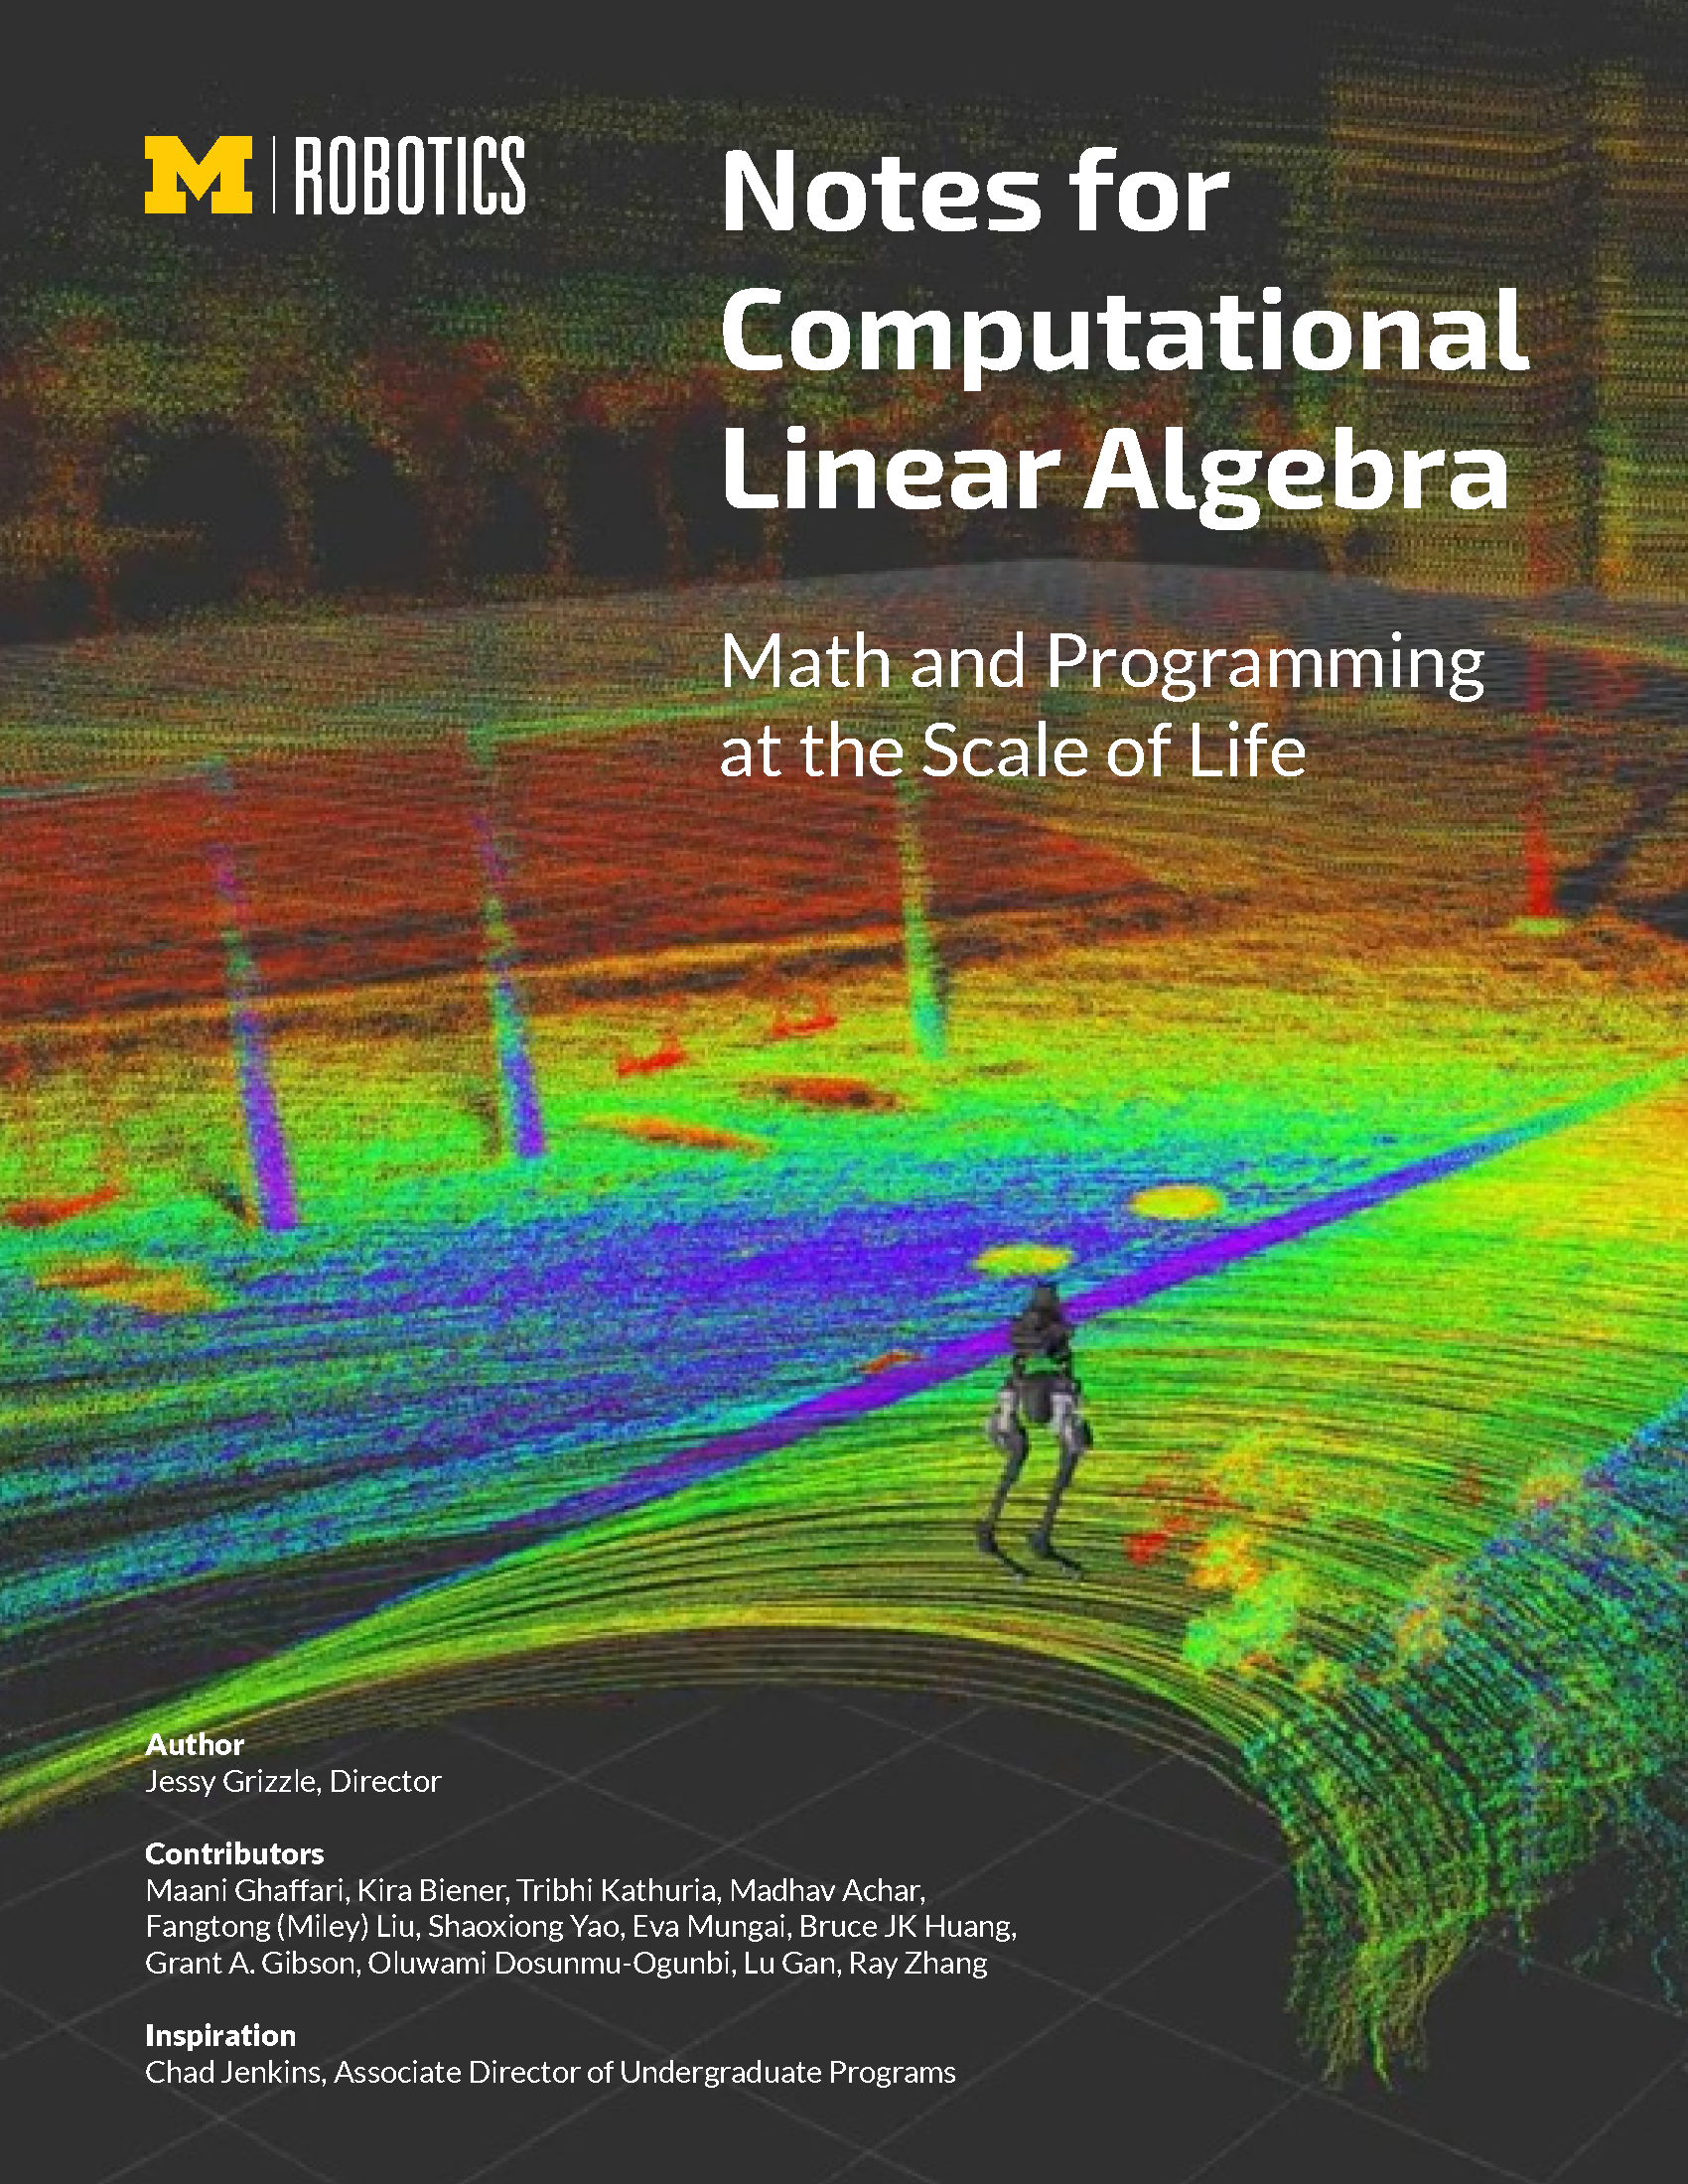
\includegraphics[scale=1.0]{rob101-cover-12-2020.png}}} % Image background
% \mbox{  }

\AddToShipoutPicture*{\put(0,0)  
{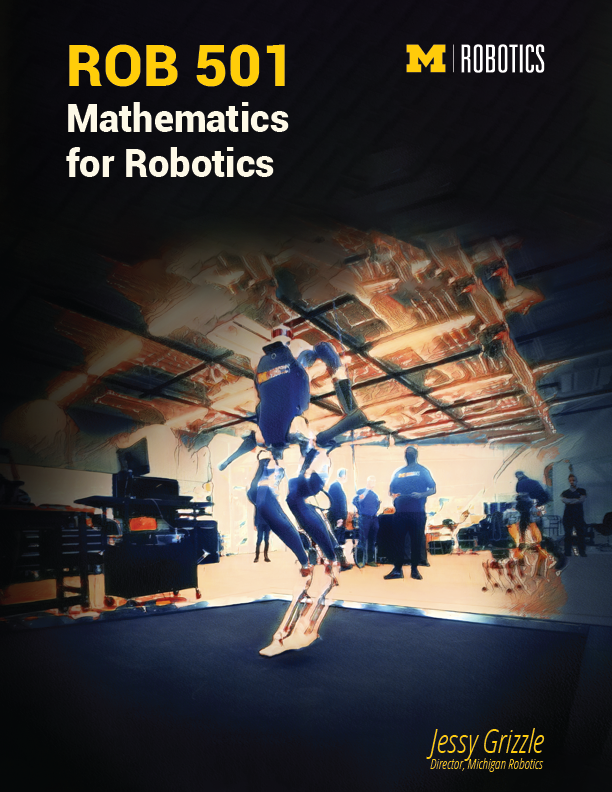
\includegraphics[scale=1.0]{graphics/501cover.png}}} % Image background
\mbox{  }

\endgroup

\clearpage


\begingroup
\thispagestyle{empty}
%\centerline
% \AddToShipoutPicture*{\put(240,50)  {\includegraphics[scale=0.35]{media_users_user_14_project_222374_images_res_cassie_image.png}}} % Image background
\AddToShipoutPicture*{\put(40,450)  {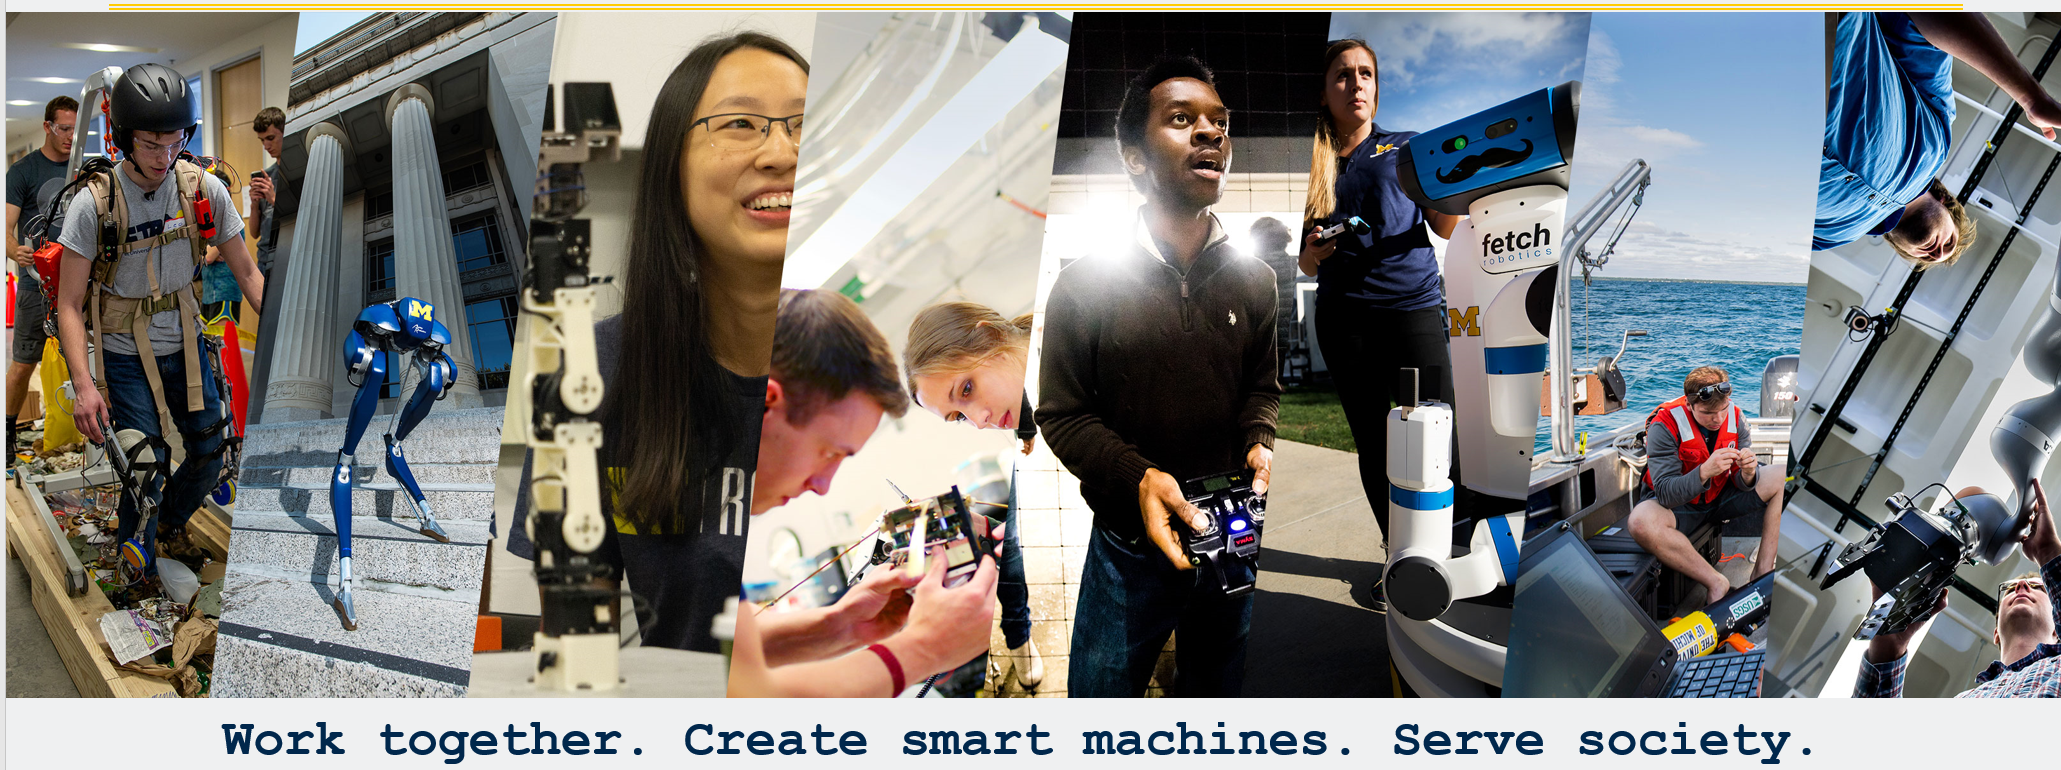
\includegraphics[scale=0.35]{WorkTogether.png}}} % Image background


~\vfill
\thispagestyle{empty}
\noindent Cover design by Dan Newman, Head of Communications, Michigan Robotics

\vspace*{2cm}
\noindent\copyright\space 2022	Jessy Grizzle,  Director of Robotics, University of Michigan	\\
\noindent \textsc{Jerry W. and Carol L. Levin Professor of Engineering\\
Elmer G. Gilbert Distinguished University Professor\\
Professor of EECS and ME}\\

%\noindent \textsc{github.com/LaurethTeX/Clustering}\\ % URL

\noindent Composed as lecture notes and piloted between August 2014 and December 2018 for use in ROB 501, Mathematics for Robotics.
\\ % License information

\noindent \textit{First release, August 31, 2022.} % Printing/edition date


\endgroup


\frontmatter
\tableofcontents
\chapter{Preface}

This collection of course notes is dedicated to all the students who have taken ROB 501 Mathematics for Robotics at the University of Michigan. The first class of students in Fall 2014 took on one of two tasks: typesetting in Latex a lecture or creating a numerically oriented HW problem in MATLAB. For their dedication, enthusiasm, and patience with the pilot version of the course, I tip my hat to Pedro Fernando, Jimmy, Vittorio, Kevin, Yuxiao, Katelyn, Omar, Ross, Jakob, Xianan, Mohammad, Jeffrey, Bo, Kurt, Josh, Xiangyu, Sulbin, Connie, Meghan, Su-Yang, Katie, Il Sun, Mia, Yong, Yunxiang, Hiroshi, Yevgeniy, Ming-Yuan, Pengcheng, and Zhiyuan. I have taken your work and expanded it into these notes. Thank you!\\

\textbf{Jessy Grizzle}\\
Winter Term, 2022
\chapter{Philosophy of the Course}

The Robotics Graduate Program was designed in 2013 and launched in 2014. The vision was to take in students from all engineering backgrounds, plus many STEM backgrounds, such as Mathematics and Physics, and prepare M.S. and Ph.D. students for fruitful careers in Industry and Academia. We knew the incoming students would have very heterogeneous preparation in Mathematics, Programming, and Hardware. To form them into a more homogeneous cohort, two first-semester courses were created, ROB 501 Mathematics for Robotics and ROB 550 Robotics Laboratory\footnote{While ROB 550 was initially charged with preparing students in the areas of embedded programming, inverse kinematics, camera calibration, path planning, encoders, motor drives, and more, later, in 2019, ROB 502 Programming for Robotics was created to relive some of the burden from ROB 550.}. After taking these two courses, the students would have adequate preparation to take courses in Sensing, Acting and Reasoning, as laid out here \url{https://robotics.umich.edu/academic-program/courses/}. The Robotics Graduate Program has worked remarkably well due to the enthusiasm of the students, staff, and faculty. \\

I accepted the charge of creating the mathematical fundamentals course, ROB 501. I interviewed the Robotics faculty in Spring 2014 to find out key topics they wanted covered. Over Summer 2014, I pared the list down and organized it into a coherent set of topics that would mostly meet the needs as identified by the faculty. To the set of topics enumerated by my colleagues, I added one additional goal, to break the students' reliance on example-based (e.g., physics-based) reasoning, and instill in them the ability to conduct \textbf{abstract reasoning}. The ability to abstract problems from a physical instantiation to a mathematical formulation provides clarity of thinking as well as being the first step in making problems amenable to algorithmic solutions. Once a student has written a problem down mathematically, they are able to search the literature for potential solutions, or understand that they have stumbled upon a new question that requires new investigations. \\

To be clear, breaking a student's reliance on physics-based reasoning really means augmenting their reasoning ability, it means giving them confidence to deal with abstract formulations of problems. The key word here is \textbf{confidence}. ROB 501 does this by doing proof after proof in every lecture. By practice and repetition, the student learns to read (relatively) complex mathematical statements, negate them, and otherwise appreciate common mathematical symbols as a precise and effective form of shorthand. To make the repetition of definitions and proofs tenable, they first practice them in the friendly environment of linear algebra. We take advantage of the fact that the vast majority of the students taking the course will be comfortable with matrix-vector arithmetic and MATLAB. While Chapter 1 introduces mathematical notation and proof techniques, these topics are not really learned until they are exercised in Chapter 2 with an abstract treatment of linear algebra, with everything proved, either in class or HW. Chapter 3 adds more abstraction, inner product spaces, but starts to provide a pay off, namely deterministic least squares problems. The students start to see how concrete optimization problems can be solved easily and precisely with the normal equations, and through HW sets, that ``practical'' problems involving functions can be solved with no essential changes to the methods. In addition, as a setup for the Kalman Filter, we derive a recursive solution to the standard (batch) least squares problem, giving us RLS.\\

Chapter 4 is meant as a mental break. While students are completing HW sets and/or exams on the previous material, we use Gram Schmidt to develop the QR Factorization, and we use orthogonal matrices and eigenvectors to derive the SVD and pause to illustrate its practical importance. While typing up these notes, I added in the LU Factorization, in part because I used it as a building block in the undergrad course, ROB 101, Computational Linear Algebra. \\

Chapter 5 sets the stage for minimum variance estimation, or non-deterministic least squares problems. We build slowly because if there is one topic with which a typical first-semester engineering graduate student struggles, it's probability. The students themselves are not to blame for this, nor are their undergraduate instructors. The topic is fundamentally very challenging. As soon we leave the confines of discrete random variables (with a finite number of possible outcomes) and enter the realm of continuous random variables, we have a choice: go down the measure theory rabbit hole or fake it. To be sure, we fake it. To clear our conscience, we are upfront about it and explain the restrictions we make to allow probabilities of events to be computed via an integral, that is, via a density and Riemann integration. This allows random vectors to be defined and the important quantities, the mean of a random vector, its covariance, and its variance. Armed with these concepts, we revisit a standard least squares problem and add a measurement noise model, leading to the Best Linear Unbiased Estimator (BLUE), and then a measurement noise model and a stochastic model for the unknown, $x$, leading to the Minimum Variance Estimator (MVE). From here, the goal is the Kalman filter. To get there, conditional probability is needed, leading to a treatment of conditional normal random vectors, which, once distilled to a set of key facts, yields the Kalman filter.\\

Chapter 6 is motivated by considering the tools required to understand the convergence of sequences and the existence of minima and maxima of functions. It's also a last pass through our proof techniques, because Chapters 4 and 5 were proof-light, being more focused on important applications of the math we had already done. We introduce the basic notions of topology, open and closed sets, in the context of normed spaces. Open and closed sets can be characterized with the notion of distance and through the convergence of sequences, showing the interplay of things that may not seem so related at a student's first glance. The contraction mapping principle is covered as are standard results on compact sets and continuous functions on compact sets. This provides general conditions that are easy to check in many engineering situations for the existence of extrema of continuous real-valued functions. These notes conclude with brief remarks on convex functions, QPs, and LPS for minimizing the one-norm and the max-norm.\\

\textbf{Jessy Grizzle}
Ann Arbor, Michigan USA
% \chapter{List of Algorithms and Methods or Things You Need Code to Do Well}
% \input{TexBookletHandouts/ListAlgorithms.tex}
\mainmatter

\chapter{Introduction to Mathematical Arguments}
\label{chap:Intro}
%*****************************************************
%Change Names and Lecture #'s here.
%*****************************************************
% {\Large \bf
% \begin{center}
% Rob 501 Fall 2014\\
% Lecture 01\\
% Typeset by:  Jimmy Amin\\
% Proofread by: Ross Hartley
% \end{center}
% }

\section*{Learning Objectives}

\begin{itemize}
\item Establish notation
\item Cover basic proof techniques, some of which may be a review
\item Set the stage for cool things to come.
\end{itemize}

\section*{Outcomes} 
\begin{itemize}
\item Learn how to read mathematical statements such as ``$\forall~\epsilon>0, \exists~\delta>0$ such that $\forall~x\in B_\delta(x_0),  ||f(x) - f(x_0)|| < \epsilon$. '' This is the definition of a function being continuous at a point $x_0$, by the way.

\item Learn how to negate mathematical statements such as the above.
 
\item Review or learn methods of proofs that we will use on a daily basis in the course.

\item In particular, overcome reluctance to use ``proof by contradiction''. 
\end{itemize}

\newpage

\section{Mathematical Notation}
    \begin{itemize}
        \item[] $\mathbb{N} = \{1,2,3,\dotsb\}$ Natural numbers or counting numbers
        \item[] $\mathbb{Z} = \mathcal{Z} = \{\dotsb, -3, -2, -1, 0, 1, 2, 3, \dotsb\}$ Integers or whole numbers
        \item[] $\mathbb{Q} = \left\{\dfrac{m}{q}~ |~ m,q \in \whole, q \neq 0, \textnormal{no common factors (reduce all fractions)}\right\}$ Rational numbers
        \item[] $\mathbb{R}$ = Real numbers
        \item[] $\mathbb{C}$ = \{$\alpha$ + $j\beta$ | $\alpha, \beta \in \real$, $j^2$ = -1\} Complex numbers
        \item[] $\forall$ means ``for every'', ``for all'', ``for each''
        \item[] $\exists$ means ``for some", ``there exist(s)'', ``there is/are'', ``for at least one''
        \item[] $\in$ means ``element of'' as in ``$x\in A$'', i.e., $x$ is an element of the set $A$
        \item[] $\sim$ denotes ``logical not''.  You will also often see $\neg$. We'll use both in these notes. 
        \item[] $p \implies q$ means ``if the logical or mathematical statement  $p$ is true, then the statement $q$ is true''
        \item[] $p \iff q$ means ``$p$ is true if, and only if , $q$ is true''. While $p \text{ iff } q$ is another way to write $p \iff q$, we will mostly avoid using it in these notes.
        \item[] $p \iff q$ is logically equivalent to 
        \begin{itemize}
            \item[] (a) $p \implies q$ and\ %\ is equal to a space
            \item[] (b) $q \implies p$
        \end{itemize}
        \item[] The \emph{contrapositive} of $p \implies q$ is $\sim q \implies \sim p$ 
        \item[] The \emph{converse} of $p \implies q$ is $q \implies p$. It is very important to note that in general, $(p \implies q)$ \emph{DOES NOT IMPLY} $(q \implies p)$, and vice-versa. If they did, we would not need $p \iff q$.
        \item[] \emph{Relation}: $(p \implies q) \Leftrightarrow (\sim q \implies \sim p)$. The two statements are logically equivalent, and hence in principle, we do not need both of them. We will see, however, that sometimes one of them is easier to use in a proof than the other. 
        \item[] \emph{Logical and}: $ p_1 \land p_2$ is read $p_1$ and $p_2$. It is true when both $p_1$ and $p_2$ are true. 
                \item[] \emph{Logical or}: $ p_1 \lor p_2$ is read $p_1$ or $p_2$. It is true when at least one of $p_1$ and $p_2$ is true. We do not use ``exclusive or'' in this course. Hence, if \textbf{T} stands for true and \textbf{F} for false, then $ \textbf{T}  \lor \textbf{T} = \textbf{T}  \lor \textbf{F} = \textbf{F}  \lor \textbf{T}  = \textbf{T} $.
        \item[] Q.E.D. or QED is an abbreviation of the Latin ``quod erat demonstrandum'' which means ``thus it was demonstrated''; it is used to alert the reader that a proof has been completed.  Nowadays, you more frequently see $\square$ or $\blacksquare$ instead of QED. 
    \end{itemize}
    
    \textbf{Warning:} In the beginning, it is quite frequent that students confuse the meanings of \emph{contrapositive} and \emph{converse}. Just be careful. With practice, it becomes second nature. The fact that they both start with ``con-'' is not helpful!

\section{Vocabulary} 
The following definitions borrow liberally from Math 299, Michigan State University, \url{https://users.math.msu.edu/users/duncan42/AxiomNotes.pdf}\\

\textbf{Meanings:}
\begin{itemize}
\item Definition : An explanation of the mathematical meaning of a word.
\item Theorem : A statement that has been proven to be true.
\item Proposition : A less important but nonetheless interesting true statement.
\item Lemma: A true statement used in proving other true statements (that is, a less important theorem that is helpful in the proof of other results).
\item Claim: A true statement that is sometimes made as a step toward proving a theorem, in which case it is similar to a lemma. It is also sometimes used to highlight a property of a mathematical object that a reader might miss. 
For example, one might define a matrix $A$ to be \emph{invertible} if there exists a second matrix $B$ such that $A\cdot B = B \cdot A = I$, where $I$ is the identity matrix. Nowhere in this definition have we explicitly stated that $A$ must be square. Hence, you might then 
\emph{Claim:} An invertible matrix is square. And then prove the claim by using the rules (i.e., definition) of matrix multiplication.
\item Corollary: A true statement that is a ``simple'' deduction from a theorem or proposition.
\item Proof: The explanation of why a statement is true.
\item Conjecture: A statement believed to be true, but for which we have no proof. (A statement that is being proposed to be a true statement).
\item Axiom: A basic assumption about a mathematical situation, or said another way, a statement Mathematicians assume to be true. One example comes from Euclid `` two distinct parallel lines in the plane never intersect''. This is a fundamental tenet of Euclidean geometry and is false in geometries where lines are curved. Another example is the axiom that for any two integers $a$ and $b$, the symbol ``$+$'' called sum has the property $a+b=b+a$, that is, the sum of $a$ and $b$ is equal to the sum of $b$ and $a$. In this sense, axioms and definitions are very similar. Axioms are reserved for the ``bedrock'' definitions in a logical or mathematical system, the definitions on which everything else is based.  
\end{itemize}





\section{Review of Proof Techniques}

When constructing a proof of a statement, axioms, definitions, theorems, lemmas, propositions, claims, and corollaries all have the same ``power'' because they consist of true statements. It is common practice to place the most fundamental description of an idea as its definition and then to provide theorems that show how to check, compute, or apply the property in the definition.

\subsection{Direct Proofs}
A proof is \emph{direct} if the result is obtained by directly applying ``simple rules of logic'', such as $p \implies q$, to the given assumptions, definitions, axioms, and already known theorems. Employing the method of ``proof by contradiction'' would not be a direct proof. A better elaboration is given here \url{https://en.wikipedia.org/wiki/Direct_proof}\\

\begin{definition}
An integer $n$ is \emph{even} if $n = 2k$ for some integer $k$; $n$ is \emph{odd} if \ $n = 2k+1$ for some integer $k$. 
\end{definition} 

\begin{rem}
In a definition, the convention is that ``if'' means ``if, and only if''. \emph{It would be considered bad style (form) to write} the above definition as follows: An integer $n$ is \emph{even} if, and only if $n = 2k$ for some integer $k$; $n$ is \emph{odd} if, and only if \ $n = 2k+1$ for some integer $k$. What you have to understand is that the two meanings are identical when used in a definition. In a lemma, theorem, claim, proposition, corollary, etc., the two meanings are very different. Yes, this takes time before it becomes second nature.
\end{rem} 

\begin{example} 
Provide a direct proof that the sum of two odd integers is even.
\end{example}

\textbf{Proof:} Let $n_1$ and $n_2$ be odd integers. Then by the definition of odd, there exist integers $k_1$ and $k_2$ such that
    \begin{align*}
        n_1 &= 2k_1+1\\
        n_2 &= 2k_2+1.
    \end{align*}
Then using the rules of arithmetic, 
    \begin{equation*}
        n_1+n_2 = (2k_1+1) + (2k_2+1) = 2(k_1+k_2+1).
    \end{equation*}
Because $k_1+k_2+1$ is the sum of three integers, it is also an integer, and therefore $2(k_1+k_2+1)$ is by definition, an even integer. Because $n_1+n_2=2(k_1+k_2+1)$, it is even. 
\Qed

\vspace*{.2cm}

Did we really need to say the last line in the proof, namely, ``Because $n_1+n_2=2(k_1+k_2+1)$, it is even''? It's a matter of taste. A proof is supposed to convince a skeptical reader that something is true. Sometimes, when writing a paper, you do have to restate the obvious to ensure that a reviewer does not miss it. 



\subsection{Proof by Contrapositive:} A proof by \emph{contrapositive} means that to establish $p \implies q$, we prove its logical equivalent, $\sim q \implies \sim p$. Once you have written down what is $\sim q$ and what is $\sim p$, the proof often proceeds like a direct proof. 

\vspace*{.2cm}
\begin{example} 
\label{ex:nSquaredEven}
Let $n$ be an integer. Prove that if $n^2$ is even, then $n$ is even.
\end{example}

\textbf{Proof:} In the beginning of your proof writing career, it is highly recommended to explicitly write down what is $p$ and what is $q$. This helps you to understand what you are trying to show and what is/are the given hypothesis(eses).\\

\begin{itemize}
    \item $p = (n^2 \text{ is even})$. Hence, $\sim p = (n^2 \text{ is odd})$.
   \item $q = (n \text{ is even})$. Hence, $\sim q = (n \text{ is odd})$.
\end{itemize}
    Our proof of $p \implies q$ is to show $\sim q \implies \sim p$, that is, if $n$ is odd, then $n^2$ is odd.  Hence, let $n$ be an odd integer. By the definition of $n$ being odd, there exists an integer $k$ such that $ n = 2k+1$. Therefore,
 $$n^2 = (2k+1)^2 = 4k^2 + 4k + 1 = 2(2k^2+2k)+1.$$
    Because $(2k^2+2k)$ is an integer, we are done. 
\Qed

\vspace*{.2cm}

Here, we simply took it as ``obvious to the most casual observer'' that once we arrived at $n^2 = 2m+1$ for $m=2k^2+2k$, that it was game over, we've said enough to convince ``anyone'' that $n^2$ is odd. Was it enough for you? 

\subsection{Proof by Exhaustion} 

Proof by \emph{exhaustion} means to reduce the proof to a finite number of cases, and then prove each case separately. As its name suggests, these proofs can be tedious at times. The \emph{Famous Four Color Problem} \url{https://en.wikipedia.org/wiki/Four_color_theorem} was proved by using computer algebra to reduce the problem to checking a finite number of map cases, and then checking them one by one. In particular, 1,834 map configurations (later reduced to 1,482) had to be checked one by one and took a computer of its day over a thousand hours. \\

On occasion, we will do a proof by exhaustion. For us, four cases will already be a lot!

\subsection{Proofs by Induction}

There are two forms of proof by \emph{induction}, that are in fact equivalent. Most engineers only know one, the first one:\\

 \textbf{First Principle of Induction (Standard Induction):}~ Let $P(n)$ denote a statement about the natural numbers with the following properties:
        \begin{itemize}
            \item[] (a) \textbf{Base case:} $P(1)$ is true
            \item[] (b) \textbf{Induction hypothesis:} If $P(k)$ is true, then $P(k+1)$ is true.
        \end{itemize}
Then $P(n)$ is true for all $n \geq 1$. \\

\begin{rem}
Suppose the base case involves an integer $k_0 \neq 1$. Then you can re-index things and reduce it to the base case having $k_0=1$. Alternatively, you assume that $P(k)$ true for $k \ge k_0$ implies  $P(k+1)$ is true, and then you get $P(n)$ is true for all $n \geq k_0$. A common mistake is to not use the correct base case. For an example, you should read about how ``to prove by induction'' that all horses are the same color \url{https://en.wikipedia.org/wiki/All_horses_are_the_same_color}. 
\end{rem} 


    \vspace*{.2cm}
\begin{example} 
Let's prove the \textbf{Claim:}  For all $n \geq 1$, $1+3+5+\dotsb+(2n-1)=n^2$.
\end{example}

\textbf{Proof:} 

    \begin{itemize}
    \item \underline{Step 0:} Write down $P(k)$: $1+3+5+\dotsb+(2k-1)=k^2$. 
        \item \underline{Step 1:} Check the base case, $P(1)$: For  $k=1$, we have that $ 1 = 1^2 $, and hence the base case is true. 
        \item \underline{Step 2:} Show the induction hypothesis is true. That is, using the fact that $P(k)$ is true, show that $P(k+1)$ is true. Often, this involves re-writing $P(k+1)$ as a sum of terms that show up in $P(k)$ and another term.\\
  
    \end{itemize}
 
 For us,  
 $$P(k+1): 1+3+5+\dotsb+(2k-1)+(2(k+1)-1)=(k+1)^2. $$
For the induction step, we assume that
$$
        P(k): = 1+3+5+\dotsb+(2k-1)=k^2 
$$
is true and thus $P(k+1)$ is true if, and only if 
$$ 
k^2 +(2(k+1)-1) =(k+1)^2.
$$
Using the known (and accepted) rules of algebra, we check that
$$       
k^2 + (2(k+1)-1) = k^2+2k+2-1 = k^2+2k+1 = (k+1)^2,
$$
and hence $P(k+1)$ is true. Because we have shown that $P(1)$ is true and for all $k\ge 1$, $P(k) \implies P(k+1)$, by the Principle of Induction, we conclude that for all $k\ge 1$,
$$ 1+3+5+\dotsb+(2k-1)=k^2.$$
\Qed
\vspace*{.2cm}


\begin{rem}
When the base case $P(1)$ seems so totally trivial that you are unsure whether there is anything to show, it's OK to check $P(2)$, just to convince yourself that it is true too. In our case you would check $P(2): 1 + 3 = 2^2 $; since this is easily established to be true, you may now be more confident of your proof. If you do one more, $P(3): 1 + 3 + 5 = 3^3$, you are now on a roll and ready to attack the general case by induction. Bottom line: In the beginning, it's natural to be tentative when you do a proof. It takes practice to learn the art of proving things. When you write a proof, we will not take off points for doing a bit more work than is strictly required. We understand that you are slowly building up your confidence.
\end{rem} 

      
\textbf{Warning:} When you seek to establish the \emph{induction hypothesis}, that $P(k+1) \implies P(k)$, you need to make sure that your reasoning works for all $k$, including the base case, $k=1$. In the infamous ``all horse are the same color proof (spoof)'', the statement $P(1) \implies P(2)$ fails. People overlook it by starting at $P(2) \implies P(3)$ or they make a mistake on $P(1) \implies P(2)$. Oooops! \\


\noindent \textbf{Second Principle of Induction (Strong Induction):}~ Let $P(n)$ be a statement about the natural numbers with the following properties:
    \begin{enumerate}
        \item[] (a) \textbf{Base Case:} $P(1)$ is true.
        \item[] (b) \textbf{Induction hypothesis:} If $P(j)$ is true for all $1\leq j\leq k$, then $P(k+1)$ is true.
    \end{enumerate}
Then $P(n)$ is true for all $n\geq 1$ (or, $n$ greater than or equal to the  $n_0$ used in the Base Case).\\

\begin{rem}
You can see why it is sometimes called \emph{Strong Induction:}  we have access to all of the logical statements $P(j)$ up to, and including, $P(k)$, when we are trying to prove the induction step $P(k+1)$ is true. We will show a bit later that the two principles of induction are logically equivalent. Nevertheless, sometimes one method is easier to apply than the other.
\end{rem}

\begin{definition}
A natural number $n \ge 2$ is \emph{composite} if it can be factored as $n=a\cdot b$, where $a$ and $b$ are natural numbers satisfying $1 < a,  b < n$. Otherwise, $n$ is \emph{prime}.
\end{definition} 

\begin{rem}
It follows from the above definition that a natural number greater than or equal to two is either prime or composite, and it cannot be both. The first prime number is $2$. What is the number $1$?
\end{rem} 

\vspace*{.2cm}
\begin{example} 
Let's prove the \textbf{Theorem}: (Fundamental Theorem of Arithmetic) Every natural number $n\geq 2$ can be factored as a product of one or more primes.
\end{example}

\textbf{Proof:} 

    \begin{itemize}
    \item \underline{Step 0:} We write down the statements. For $k \ge 2$, $P(k)$: there exist $i_k \ge 1$ and prime numbers $p_1, p_2, \ldots, p_{i_k}$ such that the product  $p_1 \dotsb p_{i_k} = k$. 
        \item \underline{Step 1:} Check the base case, $P(2)$: For  $k=2$, we have that $ 2 = 2$, and hence the base case is true. 
        \item \underline{Step 2:} Show the induction hypothesis is true. That is, using the fact that $P(j)$ is true for $1 \le j \le k$, show that $P(k+1)$ is true, that is, $k+1$ can be expressed as a product of primes. 
         There are two cases:
    \begin{enumerate}
    \renewcommand{\labelenumi}{(\alph{enumi})}
        \setlength{\itemsep}{.1cm}
        \item \underline{Case 1:} $k+1$ is prime. In this case, we are done because $k+1$ is already the product of one prime, namely itself.
        \item \underline{Case 2:} $k+1$ is composite. Then, there exist two natural numbers $a$ and $b$, $2\le a, b \le k$, such that $k+1 = a \cdot b$. \\
        
         Because $a$ and $b$ are natural numbers that are greater than or equal to $2$ and less than or equal to $k$, by the induction step:
    \begin{align*}
   P(a) \implies      a &= p_1 \cdot p_2 \cdot \dotsb \cdot p_{i_a}, \text{ for some primes } p_i\\
   P(b) \implies      b &= q_1 \cdot q_2 \cdot \dotsb \cdot q_{j_b}, \text{ for some primes } q_j
    \end{align*}
Hence, $a\cdot b = (p_1 \cdot p_2 \cdot \dotsb \cdot p_{i_a})\cdot (q_1 \cdot q_2 \cdot \dotsb \cdot q_{j_b})$, which is a product of primes.
    \end{enumerate}
    \end{itemize}
    
\Qed   

\vspace*{.2cm}

Strong Induction was useful here because we needed to ``reach back'' and use our statements $P(j)$ for values of $j$ not equal to $k$. If we relied only on Ordinary Induction, we would have been stuck. This raises the question again, is Strong Induction really more powerful than Ordinary Induction? The answer is NO, it is just sometimes more convenient. \\

\textbf{Equivalence of Strong and Ordinary Induction:} Let $P(k)$ be the set of logical statements that are used with Strong Induction. Then the induction step is equivalent to
\begin{equation}
\label{eq:WeakEqualsStong}
   (P(1) \land P(2) \land \cdots \land P(k)) \implies P(k+1), 
\end{equation} 
because we assume that $P(j)$ is true for $1 \le j \le k$. Next, you can note that \eqref{eq:WeakEqualsStong} is equivalent to 
\begin{equation}
\label{eq:WeakEqualsStong02}
   P(1) \land P(2) \land \cdots \land P(k) \implies  P(1) \land P(2) \land \cdots \land P(k) \land P(k+1), 
\end{equation} 
because if $P(1) \land P(2) \land \cdots \land P(k) = \textbf{T}$, then 
$$( P(1) \land P(2) \land \cdots \land P(k) \land P(k+1) = \textbf{T})  \iff (P(k+1) =  \textbf{T}).$$
It follows that Ordinary Induction on 
$$ Q(k):= P(1) \land P(2) \land \cdots \land P(k)$$
is equivalent to Strong Induction on $P(k)$. \\

If we return to our proof of the Fundamental Theorem of Arithmetic, then what is $Q(k)$? Well, $Q(k)$ true means that $P(1), P(2), \ldots, P(k)$ are all true, and hence
$$Q(k): \text{ for all integers } 2 \le j \le k, \text{ there exist primes } p_1, p_2, \ldots, p_{i_j}, \text{ such that } j = p_1 \cdot p_2 \cdots p_{i_j}.$$
The proof of the induction step $Q(k) \implies Q(k+1)$ is then identical to the proof we gave for $P(1) \land \cdots \land P(k) \implies P(k+1).$


\vspace*{.2cm}

\subsection{Proof by Contradiction} 

\begin{definition}
A \emph{logical contradiction}, or \emph{contradiction} for short, is a logical statement $R$ such that $R \land (\sim R) = \textbf{T}$. 
\end{definition} 

Initially, students tend to dislike proofs by contradiction. It seems to be a contradiction to logical thinking that such a method of proof can even be correct! A statement that is both true and false is called a \emph{contradiction}. The basis for a \emph{proof by contradiction} is that if you start with only true statements and correctly apply the rules of logic, you cannot generate a contradiction. Hence, if you start with a statement, say $p$, and through valid application of the rules of logic, arrive at a second statement, say $R$ that is both \textbf{T} and \textbf{F}, then the statement $p$ must be false.  We can write this as
$$ \big( p \implies \left(\exists~R  \text{ such that } R \land (\sim R) = \textbf{T}\right) \big) \iff p = \textbf{F}. $$
Only false statements can generate contradictions.\\

\textbf{The game plan for a proof by contradiction:} We want to show that a statement $p$ is true. We assume instead that the statement is false. On the basis of $p$ being false, we derive a ``contradiction'', meaning some statement $R$ that we show to be both true and false. We conclude that $\sim p$ is false, because it led to a contradiction. Hence, $p$ must be true.\\

Once we do a few examples, it becomes much easier to digest. 

\vspace*{.2cm}

\begin{example}
Use proof by contradiction to show that $\sqrt{2}$ is an irrational number.
\end{example} 

\vspace*{.2cm}

\textbf{Proof:} Our statement is $p: \sqrt{2}$ is irrational. We assume $\sim p: \sqrt{2}$ is rational. We seek to show that this leads to the existence of a statement $R$ that is both true and false, a contradiction. \\

If $\sqrt{2}$ is rational, then there exist natural numbers $m$ and $n$ such that 
\begin{itemize}
    \item $m$ and $n$ have no common factors, 
    \item $n \neq 0$, and 
\end{itemize}
\begin{equation}
\label{eq:Euclid01}
        \sqrt{2} = \frac{m}{n}.
\end{equation}
All we have done is apply the definition of a rational number. Next, we square both sides of \eqref{eq:Euclid01} to arrive at  
$$ \left(2 = \frac{m^2}{n^2} \right) \implies \left(2n^2 = m^2 \right) \implies \left(m^2\textnormal{ is even}\right).$$ 
From our result in Example~\ref{ex:nSquaredEven}, we deduce that $m$ must be even, and hence there must exist an integer $k$ such that $m=2 k$.\\

From $2 n^2 = m^2$, we deduce that 
$$ \left(2 n^2 = (2 k)^2 \right) \implies \left(2 n^2 = 4 k^2 \right) \implies \left( n^2 = 2 k^2 \right)  \implies n^2  \textnormal{ is even}.$$
Once again appealing to our result in Example~\ref{ex:nSquaredEven}, we deduce that $n$ must be even, and hence there must exist an integer $j$ such that $n=2 j$.\\

Because both $m$ and $n$ are even, they have $2$ as a common factor, which is a contradiction to $m$ and $n$ have no common factors. \\

Because we arrived at this contradiction from the statement ``$\sqrt{2}$ is rational'', we deduce that ``$\sqrt{2}$ is rational'' must be false. Hence, $\sqrt{2}$ is irrational.
\Qed.

\vspace*{.2in}

\textbf{Here is a blow by blow recap of the proof.} 
\begin{itemize}
    \item We define $p: \sqrt{2}$ is an irrational number.

\item  We start with the assumption $(\sim p = \textbf{T})$, that is, $\sqrt{2}$ is a rational number.
\item  Based on that assumption, we can deduce there exist integers $m$ and $n$, $n\neq 0$,  such that $\sqrt{2}=\frac{m}{n}$ and $m$ and $n$ do not have a common factor.
\item We now define ($R:$ $m$ and $n$ do not have a common factor) and know that $R = \textbf{T}$.
\item  However, from $\sqrt{2}=\frac{m}{n}$, we show that $m$ and $n$ have 2 as a common factor.
\item We now have $\sim R = \textbf{T}$.
\item Hence,  $ (R \land (\sim R)) = \textbf{T}$, \textcolor{red}{\bf which is a contradiction}.
\item  Conclusion: $\sim p = \textbf{T}$ is impossible, and therefore $\sim p = \textbf{F}$ .
\item  Hence, $p = \textbf{T}$ and we have proved that $\sqrt{2}$ is irrational. Pretty cool!
  \end{itemize}
  
\begin{rem}
You can also use \emph{proof by contradiction} to prove $p \implies q$. What you do is start with $p \land (\sim q)$, that is, you assume $p$ is true and $\sim q$ is true. This gives you an easy way of generating a statement that you believe to be false, and hence should lead to a contradiction. 
\end{rem}
  
  
  
\subsection{Summary:} In conclusion, we have the  following proof techniques.
    \begin{itemize}
        \item Direct Proof: $p \implies q$
        \item Proof by Contrapositive: $\sim q \implies \sim p$.   (Start with the conclusion being false, that is $\sim q$ and do logical steps to arrive at $\sim p$)
         \item Proof by Contradiction Version I: To show that $p$ is a true statement, you assume instead that $\sim p$ is true and seek a statement $R$ such that both $R$ and $\sim R$ are true, which is a contradiction. Deduce that $\sim p = \textbf{F}$ and hence $p= \textbf{T}$.
        \item Proof by Contradiction Version II: Start with $p \land (\sim q)$ (assume $p$ is true and $q$ is false. Find a statement $R$ such that both $R$ and $\sim R$ are true, which is a contradiction. Deduce that $\sim(p \land (\sim q)) = \textbf{T}$, that is, $(p \land (\sim q)) = \textbf{F}$, and hence, if $p=\textbf{T}$ then $q=\textbf{T}$. That is, $p \implies q$. 
        \item Hence, we have that $(p \implies q) \iff \sim(p \land (\sim q))$.
        \item Proof by Induction, which can be done in two forms.
        \item Proof by Exhaustion, where we enumerate a finite set of cases and check them one by one.
        \item To show $p \iff q$ is true, we need to show \textbf{both} $p \implies q$ \textbf{and its converse}, $q \implies p$. \\
        
        A rookie mistake is to prove ``both''  $p \implies q$ and its contrapositive , $\sim q \implies \sim p$. The problem here is that $\sim q \implies \sim p$ is logically equivalent to $p \implies q$ and hence all you have done is prove the same thing two different ways, which is not what you wanted to do! 
    \end{itemize}

\section{Truth Tables}

\emph{Logic Tables} or \emph{Truth Tables} are simply a list of the possible logical values of a statement's inputs followed by the corresponding value of the statement's output. Here is a \emph{truth table} for the negation operation, which has one input, $p$ and one output $\lnot p$.

\begin{center}
\Large
 \begin{tabular}{ |c|c|}
 \hline
 $p$   & $\lnot p$ \\
 \hline
T   & F\\
 \hline
F & T  \\
\hline
\end{tabular}
\end{center}

Here is a \emph{truth table} for $p \land q$, which has two inputs, $p$ and $q$, and one output $p \land q $.
\begin{center}
\Large
 \begin{tabular}{ |c|c|c|}
 \hline
$p$    & $q$  & $p \land q $\\
 \hline
T   & T & T\\
 \hline
T   & F & F\\
 \hline
F   & T & F\\
 \hline
F   & F & F\\
\hline
\end{tabular}
\end{center}

Here is a \emph{truth table} for $p \implies q$ using \emph{proof by contradiction}. The table has two inputs $p$ and $q$, and one output $\sim(p \land (\sim q))$, the last column. We include several intermediate columns required to compute the output. The input and output are highlighted in blue.
\begin{center}
\Large
 \begin{tabular}{ |c|c|c|c|c|}
 \hline
$p$    & $q$  & $\lnot q$ & $p \land \lnot q $ & $\lnot (p \land \lnot q) $\\
 \hline
\BLUE T   & \BLUE T & F & F &\BLUE T\\
 \hline
\BLUE T   &\BLUE F & T & T &\BLUE F\\
 \hline
\BLUE F   &\BLUE T & F & F & \BLUE T\\
 \hline
\BLUE F   &\BLUE F & T  & F & \BLUE T\\
\hline
\end{tabular}
\end{center}
It is remarkably easy to check that the above table is correct because it only involves logical negation and logical and. The hard part is accepting that 
$(p \implies q) \iff \lnot (p \land \lnot q)$. \\


Now we give you a partially filled \emph{truth table} for $p \implies q$, which has two inputs, $p$ and $q$, and one output $p \implies q $ and ask you to complete it. 
\begin{center}
\Large
 \begin{tabular}{ |c|c|c|}
 \hline
$p$    & $q$  & $p \implies q $\\
 \hline
T   & T & T\\
 \hline
T   & F & F\\
 \hline
F   & T & \RED ?\\
 \hline
F   & F & \RED ?\\
\hline
\end{tabular}
\end{center}

\begin{rem} Here is one way to think about it that I once found on the web and have lost the link: We define $p:$ (you score 100\% on all exams and assignments) and $q:$ (I assign you an A$^+$ grade for the course). We all agree that $p \implies q$ must be a correct statement. In fact, it should be so deep into the bedrock of grading that we can call it an axiom! It's just that until now, you maybe never thought to complete a truth table for it! So, consider the following four scenarios, which correspond to the four lines in the truth table:
\begin{itemize}
    \item[]  $p=$ you score 100\% and $q=$ your grade is an A$^+$, then $(p\implies q) = \textbf{T}$ (easy)
        \item[]  $p=$ you score 100\% and $q=$ your grade is an A$^-$, then $(p\implies q) = \textbf{F}$ (easy)
            \item[]  $p=$ you score 85\% and $q=$ your grade is an A$^+$, then $(p\implies q) = \textbf{?}$ (ask yourself, does this invalidate the statement?)
        \item[]  $p=$ you score 85\% and $q=$ your grade is an A$^-$, then $(p\implies q) = \textbf{?}$ (ask yourself, does this invalidate the statement?)
\end{itemize}
To get the answers, look at the truth table of $\lnot (p \land \lnot q)$. If this makes your head spin, don't worry about it. After we do a bunch of proofs, you can come back to this riddle. The reasoning is, once you fail to live up to the 100\% standard, then $p = \textbf{F}$. Then, no matter what grade I give you, I am not invalidating the promise, $p \implies q$. Hence, the questions marks cannot be \textbf{F}. Because we are using binary logic, $\lnot \textbf{F} = \textbf{T}$. Therefore, the question marks must be replaced with  
\textbf{T}. Pretty cool, right?
 
\end{rem} 


\section{Negating Logical Statements}

By now, you've noticed that several of the proof techniques require you to negate a logical statement. Some are super easy, such as, when $p:x >0$, you easily see that $\sim p: x \le 0$. In the beginning, for more complex statements, we recommend you first ``translate them to English (or your preferred language), negate that statement, and then ``translate'' back into math. The math symbols are simply shortcuts for word phrases, so there is nothing illogical or wrongheaded about doing negations this way. It does take more time, and with practice, you will learn to skip the ``translation'' step, altogether. 

\begin{example}
Let $p: \forall~x \in \real,~ f(x) >0$. Compute its negation.
\end{example}

\vspace*{.2cm}

\textbf{Solution:}
\begin{itemize}
    \item Math form: $p: \forall~x \in \real,~ f(x) >0$
    \item Word form: $p:$ for all $x\in \real$, $f(x) >0$
    \item Negate: $\sim p:$ not (for all $x\in \real$, $f(x) >0$)
    \item Equivalent: $\sim p:$ for some $x\in \real$, not[$f(x) >0$]
     \item Equivalent: $\sim p:$ for some $x\in \real$, $f(x) \le 0$
      \item Math form: $\sim p:~ \exists~x\in \real$, such that $f(x) \le 0$
\end{itemize}
\Qed
\vspace*{.2cm}


\vspace*{.2cm}

\begin{example}
Let $y\in \real$ and define $p: \forall~\delta>0, \exists x \in {\cal Q}$ such that $|x-y| < \delta$. Determine its negation. Recall, $\mathcal{Q}$ is the set of rational numbers.
\end{example}

\vspace*{.2cm}

\textbf{Solution:}
\begin{itemize}
    \item Math form: $p: \forall~\delta>0, \exists x \in {\cal Q}$ such that $|x-y| < \delta$
    \item Word form: $p:$ for all $\delta >0$, there exists $x \in {\cal Q}$ such that $|x-y| < \delta$
    \item Negate: $\sim p:$ not (for all $\delta >0$, there exists $x \in {\cal Q}$ such that $|x-y| < \delta$)
    \item Equivalent: $\sim p:$ for some $\delta >0$, not[there exists $x \in {\cal Q}$ such that $|x-y| < \delta$]
    %  \item Equivalent:  $\sim p:$ for some $\delta >0$, not[there exists $x \in {\cal Q}$ such that $|x-y| < \delta$]
    \item Equivalent:  $\sim p:$ for some $\delta >0$, there does not exist $x \in {\cal Q}$ such that $|x-y| < \delta$
        \item Equivalent:  $\sim p:$ there exists $\delta >0$, such that for all $x \in {\cal Q}$, not[$|x-y| < \delta$]
        \item Equivalent:  $\sim p:$ there exists $\delta >0$, such that for all $x \in {\cal Q}$, $|x-y| \ge \delta$
      \item Math form: $\sim p:~ \exists ~\delta>0, \forall  x \in {\cal Q}, |x-y| \ge  \delta$ 
\end{itemize}
\Qed
\vspace*{.2cm}

When negating statements with $\exists$ and $\forall$, here are the logical equivalents of their negations:
\begin{align*}
    \sim \forall & \iff \exists \\
    \sim \exists & \iff \forall
\end{align*}

\begin{rem}  It is better to avoid $\not \forall$ and $\not \exists$, but they are legal symbols.
\end{rem}

\vspace*{.2cm}

\begin{example}
Negate the statement $p:\forall y \in \real,  \forall~\delta>0, \exists x \in {\cal Q}$ such that $|x-y| < \delta$. 
\end{example}

\vspace*{.2cm}

\textbf{Solution:}
$\sim p: \exists y \in \real \text{ and } \exists \delta >0$ such that, $\forall~x \in {\cal Q}, |x-y| \ge \delta $.
\Qed

\vspace*{.2cm}


\section{Key Properties of Real Numbers} 

Let $A$ be a subset of the reals, $\real$.\\

\begin{definition}
An element $b\in A$ is a \emph{maximum} of $A$ if $x \le b$ for all  $x\in A$. We note that in the definition, $b$ \underline{must} be an element of $A$. We denote it by $$\max~A \text{ or } \max \{ A\}.$$
\end{definition}

It is very important to note that a \emph{max of a set may not exist}! Indeed, the set $A = \{  x\in \real~|~ 0  < x < 1\}$ does not have a maximum element. We will see later that it does not have a minimum either. This is what motivates the notions of supremum and infimum.\\

\begin{definition}
An element $b\in \real$ is an \emph{upper bound} of $A$ if $x \le b$ for all  $x\in A$.  We say that $A$  is \emph{bounded from above}.
\end{definition}

\begin{rem}
We note that in the definition of upper bound,  $b$ does NOT have to be an element of $A$.
\end{rem}

\begin{definition}
An element $b^*\in \real$ is the \emph{least upper bound} of $A$ if
\begin{enumerate}
\renewcommand{\labelenumi}{(\alph{enumi})}
\setlength{\itemsep}{.2cm}
\item $b^*$ is an upper bound, that is $\forall ~x\in A$,~$x \le b^*$, and
\item  if $b\in \real$ satisfies $ x \le b$ for all $x\in A$, then $b^* \le b$. (This means that there is no other upper bound that is strictly smaller than $b^\ast$.)
\end{enumerate}
\end{definition}

\begin{notvocab}
The least \emph{least upper bound} of $A$ is also called the \emph{supremum} of $A$ and is denoted
$$\sup A~~~\mbox{or}~~~\sup\{A\}$$
\end{notvocab} 


\begin{center}

\fbox{\fbox{\large \textbf{Key Theorem} If $A \subset \real$ is bounded from above, then $\sup\{A\}$ exists in $\real$.}}
    
\end{center}
\vspace*{.5cm} 

\begin{rem}
The rational numbers ${\cal Q}$ do not satisfy the above property, namely, sets that are bounded from above may not have a supremum within the rational numbers. Let $A \subset {\cal Q}$ be defined as
$$A:=\{ x \in {\cal Q}~|~ \exists~ n \ge 1, x + \frac{1}{n} \le \sqrt{2} \}.$$
The number $1.5 \in {\cal Q} $ is an upper bound of $A$, but there is no rational number that is a \emph{least upper bounded}. Of course, viewed as a subset of the real numbers, $A$ has a least upper bound, namely $\sqrt{2}$. This is a subtle but important difference. In fact, one can construct the real numbers from the rational numbers as the ``smallest set that (i) contains the rationals and (ii) all subsets that are bounded from above have a least upper bound, that is, a supremum. 

\end{rem} 


\begin{example} \mbox{ }
\begin{itemize}
\item $A = \{  x\in \real~|~ 0  < x < 1\}$. Then $\sup A =1$.
\item $A= \{ x\in \real~|~ x^2 \le 2\}.$ Then  $\sup A =\sqrt{2}$.
\end{itemize}
\end{example}

\begin{rem}
\textbf{(Dej\`a Vu All Over Again)} The existence of a \emph{supremum} is a special property of the real numbers. If you are working within the rational numbers, an upper bounded set may not have a \underline{rational} supremum. If you view the set as a subset of the reals, it will then have a supremum, but the supremum may be an irrational number.
\end{rem}

\vspace*{.2cm} 

\begin{example} \mbox{ }
\begin{itemize}
\item $A = \{  x\in \mathbb{Q}~|~ 0  < x < 1\}$. Then $\sup A =1$. Indeed, 1.0 is a rational number, it is an upper bound, and it less than or equal to any other upper bound; hence it is the supremum.
\item $A= \{ x\in \mathbb{Q}~|~ x^2 \le 2\}.$  Then $(1.42)^2 = 2.0164$, and thus $b=1.42$ is a rational upper bound. Also $(1.415)^2 = 2.002225$, and thus $b=1.1415$ is a smaller rational upper bound. However, there is no least upper bound within the set of rational numbers. When we view the set $A$ as being a subset of the real numbers, then there is a real number that is a least upper bound and we have $\sup A =\sqrt{2}$. This is what we mean when we say that the existence of a supremum is a special or distinguishing property of the real numbers.
\end{itemize}
\end{example}


\begin{center}

\fbox{\fbox { \parbox { .8\linewidth}{\large \noindent \textbf{Important Fact:} Suppose $A \subset \real$. If the \emph{supremum} of $A$ is in the set $A$, then it is equal to the \emph{maximum}. In fact, $$b^\ast = \max \{A\} \iff (b^\ast = \sup \{A\}) \land (b^\ast \in A). $$}}}
    
\end{center}
\vspace*{.5cm}

Everything we have done above can be repeated with \emph{minimum} replacing \emph{maximum}, \emph{greatest lower bound} replacing \emph{least upper bound}, and \emph{infimum} replacing \emph{supremum}. Consider once again a set $A \subset \real$.\\

\begin{definition}
An element $b\in A$ is a \emph{minimum} of $A$ if $b \le x$ for all  $x\in A$.
We note that in the definition,  $b$ \underline{must} be an element of $A$. We denote it by $\min~A$ or $\min \{ A\}$. \\
\end{definition}

It is important to note that a \emph{min} of a set may not exist! Indeed, the set $A = \{  x\in \real~|~ 0  < x < 1\}$ does not have a minimum element.\\

\begin{definition}
An element $b\in \real$ is a \emph{lower  bound} of $A$ if $b\le x$ for all  $x\in A$.  We say that $A$  is \emph{bounded from below}.
\end{definition}

\begin{rem}
 We note that in the definition of lower bound,  $b$ does NOT have to be an element of $A$.
\end{rem}

\begin{definition}
An element $b^*\in \real$ is the \emph{greatest lower bound} of $A$ if
\vspace*{0.2cm}
\begin{enumerate}
\item $b^*$ is a lower bound, that is $\forall ~x\in A$,~$b^* \le x$, and
\item  if $b\in \real$ satisfies $b\le x$ for all $x\in A$, then $b^* \ge b$.
\end{enumerate}
\end{definition}

\begin{notvocab}The greatest lower bound of $A$ is also called the \textbf{infimum} and is denoted
$$\inf A~~~\mbox{or}~~~\inf\{A\}$$
\end{notvocab} 



\begin{center}

\fbox{\fbox{\large \textbf{Key Theorem}  If the set $A$ is bounded from below, then $\inf~A$ exists.}}
    
\end{center}
\vspace*{.5cm} 



\begin{example} \mbox{ }
\begin{itemize}
\item $A = \{  x\in \real~|~ 0  < x < 1\}$. Then $\inf A =0$.
\item $A= \{ x\in \real~|~ x^2 \le 2\}.$ Then  $\inf A =-\sqrt{2}$.
\end{itemize}
\end{example}


\begin{rem}
 If the \emph{infimum} is in the set $A$, then it is equal to the \emph{minimum}.
\end{rem}

\begin{definition}
If a set $A\subset \real$ is not bounded from above, we define $\sup~A = +\infty$. If $A\subset \real$ is not bounded from below, we define $\inf~A = -\infty$. \emph{The symbols  $+\infty$ and $-\infty$ are not real numbers}. The \textbf{extended real numbers} are sometimes defined as
$$\real_e:=\{-\infty\} \cup \real \cup \{+\infty \}.$$
\end{definition} 


\begin{rem}
 \textbf{(Final)} Michigan's MATH 451 \emph{constructs} the real numbers from the rational numbers. This is a very cool process to learn. Unfortunately, we do not have the time to go through this material in ROB 501. The existence of supremums and infimums for bounded subsets of the real numbers is a consequence of how the real numbers are defined (i.e., constructed).
\end{rem}




\chapter{Some Highlights of Abstract Linear Algebra (or Practicing Proofs in a Safe Environment)}
\label{chap:LinearAlgebra}
\section*{Learning Objectives}

\begin{itemize}
\item Establish key definitions for fields, vectors, vector spaces, linear combinations, linear independence, subspaces, basis vectors, linear operators, matrix representations, eigenvalues and eigenvectors.
\item Initial practice with the proof techniques of the previous chapter.
\end{itemize}

\section*{Outcomes} 
\begin{itemize}
\item Understand a very general notion of vector spaces, where the vectors range from the standard column vectors in $\real^n$ to matrices and functions.

\item Understand how the notion of representing a vector with respect to a set of basis vectors establishes one-to-one relations with columns of numbers that can be used in numerical computations.

\item Understand a related notion for associating linear operators to matrices.

\item Set you up for Chapter 3 which solves best approximation problems for generalizations of the Euclidean norm.

\item Have your mind blown by the real numbers forming an infinite dimensional vector space over the field of rational numbers. 


\end{itemize}

\newpage

\section{Fields and Vector Spaces}

Mostly in this course, we work with the real numbers or the complex numbers. However, in this Chapter, as part of our push to tear you away from the familiar and confront you with more abstraction than you may have seen before, we define a general \emph{field}, ${\cal F}$. When you are first learning the abstract definition, it is good to keep a `` canonical example'' in mind, and that would be ${\cal F} = \real$.\\


\begin{definition} (Chen, 2nd edition, page 8) : A \textbf{field} consists of a set, denoted by $\mathcal{F}$, of elements called \textbf{scalars} and two operations called addition ``$+$'' and multiplication ``$\cdot$''; the two operations are defined over $\mathcal{F}$ such that they satisfy the following conditions:
    \begin{enumerate}
        \item To every pair of elements $\alpha$ and $\beta$ in $\mathcal{F}$, there correspond an element $\alpha+\beta$ in $\mathcal{F}$ called the \emph{sum} of $\alpha$ and $\beta$, and an element $\alpha \cdot \beta$ (or simply $\alpha \beta$) in $\mathcal{F}$ called the \emph{product} of $\alpha$ and $\beta$.
        \item Addition and multiplication are respectively commutative: For any $\alpha$ and $\beta$ in $\mathcal{F}$,
        \begin{align*}
            \alpha+\beta &= \beta + \alpha & \alpha\cdot\beta &= \beta\cdot\alpha
        \end{align*}
        \item Addition and multiplication are respectively associative: For any $\alpha$, $\beta$, $\gamma$ in $\mathcal{F}$,
        \begin{align*}
            \left(\alpha+\beta\right)+\gamma &= \alpha + \left(\beta+\gamma\right) & \left(\alpha\cdot\beta\right)\cdot\gamma = \alpha\cdot\left(\beta\cdot\gamma\right)
        \end{align*}
        \item Multiplication is distributive with respect to addition: For any $\alpha$, $\beta$, $\gamma$ in $\mathcal{F}$,
        \begin{align*}
            \alpha\cdot\left(\beta+\gamma\right) = \left(\alpha\cdot\beta\right)+\left(\alpha\cdot\gamma\right)
        \end{align*}
        \item $\mathcal{F}$ contains an element, denoted by $0$, and an element, denoted by $1$, such that $\alpha + 0 = \alpha$ and $1\cdot\alpha = \alpha$ for every $\alpha$ in $\mathcal{F}$.
        \item To every $\alpha$ in $\mathcal{F}$, there is an element $\beta$ in $\mathcal{F}$ such that $\alpha+\beta = 0$. The element $\beta$ is called the \emph{additive inverse}.
        \item To every $\alpha$ in $\mathcal{F}$ which is not the element 0, there is an element $\gamma$ in $\mathcal{F}$ such that $\alpha\cdot\gamma = 1$. The element $\gamma$ is called the \emph{multiplicative inverse}.
    \end{enumerate}
\end{definition}

\vspace*{.2cm}
To show a given set is a field, you must check all seven axioms. To show something is not a field, you only need to show that one of the axioms fails.      
\vspace*{.2cm}

\begin{center}
\begin{tabular}{|c|l|}
\hline
Examples of Fields& Non-examples \\ \hline
$\real$ & Irrational (Fails axiom 1) \\ \hline
$\cp$ & $2\times2$ matrices, real coeff. (Fails axiom 2) \\ \hline
$\mathbb{Q}$ & $2\times2$ diagonal matrices real coeff. (Fails axiom 7) \\ \hline
\end{tabular}
\end{center}

\vspace*{,2cm}

\begin{definition} (Chen 2nd Edition, page 9) A \textbf{vector space (or, linear space)} over a field $\mathcal{F}$, denoted by $\left(\mathcal{X},\mathcal{F}\right)$, consists of a set, denoted by $\mathcal{X}$, of elements called \textbf{vectors}, a field $\mathcal{F}$, and two operations called \textbf{vector addition} and \textbf{scalar multiplication}. The two operations are defined over $\mathcal{X}$ and $\mathcal{F}$ such that they satisfy all the following conditions:
    \begin{enumerate}
        \item To every pair of vectors $v^1$ and $v^2$ in $\mathcal{X}$, there corresponds a vector $v^1+v^2$ in $\mathcal{X}$, called the sum of $v^1$ and $v^2$ \footnote{We use superscripts $v^1, v^2, v^3$ to denote different \emph{vectors}. The superscripts \emph{do not} denote powers.}.
        \item Addition is commutative: For any $v^1,v^2$ in $\mathcal{X}$, $v^1+v^2 = v^2+v^1$.
        \item Addition is associative: For any $v^1,v^2$, and $v^3$ in $\mathcal{X}$, $\left(v^1+v^2\right)+v^3 = v^1 + \left(v^2+v^3\right)$.
        \item $\mathcal{X}$ contains a vector, denoted by \textbf{0}, such that \textbf{0}$ + v = v$ for every $v$ in $\mathcal{X}$. The vector \textbf{0} is called the zero vector or the origin.
        \item To every $v$ in $\mathcal{X}$, there is a vector $\bar v$ in $\mathcal{X}$, such that $v + \bar v = 0$.
        \item To every $\alpha$ in $\mathcal{F}$, and every $v$ in $\mathcal{X}$, there corresponds a vector $\alpha\cdot v$ in $\mathcal{X}$ called the \emph{scalar product} of $\alpha$ and $v$.
        \item Scalar multiplication is associative: For any $\alpha, \beta$ in $\mathcal{F}$ and any $v$ in $\mathcal{X}$, $\alpha\cdot\left(\beta\cdot x\right) = \left(\alpha\cdot\beta\right)\cdot v$.
        \item Scalar multiplication is distributive with respect to vector addition: For any $\alpha$ in $\mathcal{F}$ and any $v^1,v^2$ in $\mathcal{X}$, $\alpha\cdot\left(v^1+v^2\right) = \alpha\cdot v^1 + \alpha\cdot v^2$.
        \item Scalar multiplication is distributive with respect to scalar addition: For any $\alpha ,\beta$ in $\mathcal{F}$ and any $v$ in $\mathcal{X}$, $\left(\alpha+\beta\right)\cdot v = \alpha\cdot v + \beta\cdot v$.
        \item For any $v$ in $\mathcal{X}$, $1\cdot v=v$, where $1$ is the element $1$ in $\mathcal{F}$.
    \end{enumerate}
        
\end{definition} 

\vspace*{.2cm}

\begin{example} 
 $\mathcal{F} = $ field, $\mathcal{X} = $ set of vectors
    \begin{enumerate}
        \item Every field forms a vector space over itself. $\left(\mathcal{F},\mathcal{F}\right)$. Examples: $\left(\real,\real\right)$, $\left(\cp,\cp\right)$, $\left(\mathbb{Q},\mathbb{Q}\right)$.
        \item $\left(\cp,\real\right)$, meaning $\mathcal{X} = \cp$, $\mathcal{F} = \real$, is a vector space. This works because a real scalar $\alpha \in \mathcal{F}=\real$ times a complex number $v \in \mathcal{X}=\cp$ yields a complex number $\alpha \cdot v \in \mathcal{X}=\cp$. 
        \item $\mathcal{F} = \real$, and $\mathcal{X} = \left\{f:D\to\real\right\} = \left\{\mbox{functions from } D \mbox{ to } \real \right\}$, where $D \subset \real$ (examples: $D = \left[a,b\right]; D = \left(0,\infty\right); D = \real$) with vector addition and scalar times vector multiplication defined as follows:
        \begin{enumerate}
            \item $\forall~ f,g\in\mathcal{X}$, define $f+g \in \mathcal{X}$ by $\forall t\in D,\ \left(f+g\right)(t) := f(t) + g(t)$;
            \item  $\forall~ f \in\mathcal{X}$ and $\alpha\in\real$, define $\alpha\cdot f\in\mathcal{X}$ by $\forall t\in D, \left(\alpha\cdot f\right)(t) := \alpha\cdot f(t)$.
            \end{enumerate}
            Note that we are using the known properties of addition and multiplication of real numbers to define what we mean by the sum of two functions and the product of a real number and a function. To prove that $(\mathcal{X}, \mathcal{F})$ is a vector space, you must check all ten of the axioms. We'll check \#8 to illustrate what as to be done: we need to show that  scalar multiplication is distributive with respect to vector addition: 
            $$\alpha \cdot (f + g) = \alpha \cdot f + \alpha \cdot g.$$ 
            Our method of proof is to show that the left hand side (LHS) equals the right hand side (RHS) when 
            \begin{itemize}
                \item we use the definition of a function evaluated at a point $t$, and
                \item we subsequently apply the known definitions for sums and products of real numbers.
            \end{itemize}
            Let $t \in D$, then 
               \begin{enumerate}
            \item LHS: $[\alpha \cdot (f+g)](t): = \alpha \cdot[f + g](t) = \alpha \cdot [f(t) + g(t)] = \alpha \cdot f(t) + \alpha \cdot g(t)$.
            \item RHS: $[\alpha \cdot f + \alpha \cdot g](t):= [\alpha \cdot f](t) + [ \alpha \cdot g](t) = \alpha \cdot f(t) + \alpha \cdot g(t)$
            \item Hence, LHS = RHS and we are done.
            \end{enumerate}
        \item Let $\mathcal{F}$ be a field and define $\mathcal{X}:=\mathcal{F}^n$ the set of n-tuples written as columns
        \begin{align*}
            \mathcal{F}^n: = \left\{\left.\begin{bmatrix} \alpha_1 \\ \vdots \\ \alpha_n \end{bmatrix} \right| \alpha_i \in \mathcal{F}, 1 \leq i \leq n\right\}
        \end{align*}
        Then $(\mathcal{F}^n, \mathcal{F})$ is a vector space with the operations
        \begin{enumerate}
            \item Vector Addition: $\begin{bmatrix} \alpha_1 \\ \vdots \\ \alpha_n \end{bmatrix} + \begin{bmatrix} \beta_1 \\ \vdots \\ \beta_n \end{bmatrix} = \begin{bmatrix} \alpha_1 + \beta_1 \\ \vdots \\ \alpha_n + \beta_n \end{bmatrix}$
            \item Scalar Multiplication: $\alpha\cdot x = \begin{bmatrix} \alpha x_1 \\ \vdots \\ \alpha x_n \end{bmatrix}$
        \end{enumerate}
        \item In a similar manner, one can take $\mathcal{X} := \mathcal{F}^{n\times m} = \left\{n\times m \mbox{ matrices with coefficients in } \mathcal{F}\right\}$ with vector addition and scalar times vector multiplication defined in the obvious ways. Hence, matrices can be viewed as vectors. 
        
        \item $(\real,\mathbb{Q})$ is a vector space. It is not particular useful in Robotics. It's kind of cool to think about. The set of vectors is $\real$. Clearly, the sum any two real numbers is again a real number, and hence a vector. The usual scalar times vector multiplication works because the product of a rational number and a real number is a real number, and hence is a vector. 
    \end{enumerate}
    \end{example}

\vspace*{.2cm}

    \begin{nonexample} \mbox{ }
    \begin{enumerate}
        \item Take $ \mathcal{X} = \real, \mathcal{F} = \cp$. Then $(\mathcal{X}, \mathcal{F}):=\left(\real,\cp\right) $ fails the definition of scalar multiplication (and others).
        \item $ \mathcal{X} = \left\{x\geq 0,x\in\real\right\}, \mathcal{F} = \real $. Then  $(\mathcal{X}, \mathcal{F})$ fails the definition of scalar multiplication (and others).
        
        \item $(\mathbb{Q}, \real)$ is a not vector space. The set of vectors is $\mathbb{Q}$. Clearly, the sum any two rational numbers is again a rational number, and hence a vector. The usual scalar times vector multiplication fails, however,  because the product of a real number and a rational number is a real number, and hence is not a vector.
        
    \end{enumerate}
        
\end{nonexample}

\vspace*{.2cm}

\section{Subspaces}

\begin{notation}
 Let $A$ and $B$ be sets. Then 
\begin{itemize}
    \item $(A \subset B) \iff (a\in A \implies a \in B)$
    \item $(A = B) \iff (A \subset B \text{ and } B \subset A)$
\end{itemize}
\end{notation}
In ROB 501, we do not use the notion of $A$ being a \emph{strict subset} of $B$, which in some books is denoted as $A \subsetneq B$ or $A \subsetneqq B$. Please do not use such notation in your HWs or exams. \\

\begin{definition}
 Let $\left(\mathcal{X},\mathcal{F}\right)$ be a vector space, and let $\mathcal{Y}$ be a subset of $\mathcal{X}$. Then $\mathcal{Y}$ is a \textbf{subspace} if using the rules of vector addition and scalar multiplication defined in $\left(\mathcal{X},\mathcal{F}\right)$, we have that $\left(\mathcal{Y},\mathcal{F}\right)$ is a vector space.
\end{definition}

\begin{rem}
To show that a set is a subspace using the definition, you have to check axioms 1 to 10. To show that a set is NOT a subspace, you just need to show that one of the axioms is violated. The first thing you should always check is that $0 \in \mathcal{Y}$.  
\end{rem} 

% \textbf{Proposition: } 
\begin{prop}
(Tools to check that something is a subspace)
Let $\left(\mathcal{X},\mathcal{F}\right)$ be a vector space and $\mathcal{Y}\subset\mathcal{X}$.
Then, the following are equivalent (TFAE):
    \begin{enumerate}
        \renewcommand{\labelenumi}{(\alph{enumi})}
        \setlength{\itemsep}{.1cm}
        \item $\left(\mathcal{Y},\mathcal{F}\right)$ is a subspace of $\left(\mathcal{X},\mathcal{F}\right)$.
        
        \item $\forall v^1,v^2\in\mathcal{Y}, v^1+v^2\in\mathcal{Y}$ (closed under vector addition), and $\forall y\in\mathcal{Y}$ and $\alpha\in\mathcal{F},\alpha y\in\mathcal{Y}$ (closed under scalar multiplication).
        
        \item $\forall v^1,v^2\in\mathcal{Y}$, $\forall \alpha\in\mathcal{F}, \alpha\cdot v^1+v^2 \in \mathcal{Y}$.
        
             \item $\forall v^1,v^2\in\mathcal{Y}$, $\forall \alpha_1, \alpha_2 \in\mathcal{F}, \alpha_1 \cdot v^1+ \alpha_2 \cdot v^2 \in \mathcal{Y}$. 
    \end{enumerate}
\end{prop}
\vspace*{.2cm}

Because (a) through (d) are equivalent, you can use any of (b) through (d) to show that (a) is true.\\

\begin{example} \mbox{ }
\begin{itemize}
    \item  $\left(\mathcal{X},\mathcal{F}\right) := (\real^2, \real)$ and $\mathcal{Y} := \left\{ \left[ \begin{array}{c} \beta\\ 2 \beta \end{array} \right] ~ \big|~ \beta \in \real \right\}\subset \mathcal{X}$. For $v^1, v^2 \in \mathcal{Y}$, we have
    $$ \underbrace{\left[ \begin{array}{c} \beta_1\\ 2 \beta _1\end{array} \right]}_{v^1} +  \underbrace{\left[ \begin{array}{c} \beta_2\\ 2 \beta_2 \end{array} \right]}_{v^2} =  \left[ \begin{array}{c} \beta_1 + \beta_2\\ 2 (\beta_1 + \beta_2) \end{array} \right] \in \mathcal{Y} $$
    and for  $v \in \mathcal{Y}$ and $\alpha \in \real$,
    $$ \alpha \underbrace{\left[ \begin{array}{c} \beta\\ 2 \beta\end{array} \right]}_{v} =\left[ \begin{array}{c} \alpha  \beta\\ 2 (\alpha  \beta) \end{array} \right] \in \mathcal{Y} .
    $$
    Hence, by the Proposition, $\mathcal{Y}$ is a subspace.
    
    \item $\left(\mathcal{X},\mathcal{F}\right), \mathcal{F} = \real$, where $\mathcal{X} = \left\{f: \real \to \real\right\}$, and we define 
    $$\mathcal{Y}:= \mathcal{P}(t):=\left\{ \mbox{polynomials in t with real coefficients} \right\}$$
is a subspace because we know that the sum of two polynomials with real coefficients is another polynomial with real coefficients, and the product of a real number and a polynomial with real coefficients is once again a polynomial with real coefficients. \\

\item In a similar manner, you can check that  $ \widetilde{\mathcal{Y}} := \left\{ f: \real \to \real ~|~ f \text{ is differentiable }, \frac{d}{dt}f \equiv 0 \right\}$ is a subspace of $\mathcal{X}$.
\end{itemize}
    
\end{example}

\vspace*{.2cm}

\begin{nonexample}
 We take $(\mathcal{X}, \mathcal{F}):= (\real^2, \real)$ and define 
$\mathcal{Y} := \left\{ \left[ \begin{array}{c} \beta\\ 2 \beta \end{array} \right] + \left[ \begin{array}{c} 1\\ 0 \end{array} \right]~ \big|~ \beta \in \real \right\}\subset \mathcal{X}$. Then $0 \not \in \mathcal{Y}$ and hence $\mathcal{Y}$ is not a subspace. In a similar manner, $ \widehat{\mathcal{Y}} := \left\{ f: \real \to \real ~|~ f(2)=1.0 \right\}$ is not a subspace because it does not contain the zero vector, that is, a function that is zero for all $t\in \real$.
    
\end{nonexample}


\section{Linear Combinations and Linear Independence}

\begin{definition} Let $(\mathcal{X},\mathcal{F})$ be a vector space. A \textbf{linear combination} is a \textbf{finite sum} of the form $\alpha_1v^1+\alpha_2v^2+\ldots+\alpha_nv^n$ where $n\geq 1, \alpha_i \in \mathcal{F}, v^i\in\mathcal{X}$. \textcolor{red}{\bf To be extra clear, a sum of the form $\sum_{i=1}^{\infty} \alpha_i v^i$ is not a linear combination because it is not finite.} 
\end{definition}

\begin{definition} A finite set of vectors $\{v^1, \dots, v^k\}$ is \textbf{linearly dependent} if $~\exists\alpha_1, \ldots \alpha_k\in\mathcal{F}$ \textbf{not all zero} such that $\alpha_1v^1+\alpha_2v^2+\ldots+\alpha_kv^k=0$. Otherwise, the set is \textbf{linearly independent}.
\end{definition}


\begin{rem} Suppose $\{v^1, \dots, v^k\}$ is a linearly dependent set. Then, $\exists\alpha_1, \dots, \alpha_k$ are not all zero such that $$\alpha_1v^1+\alpha_2v^2+\ldots+\alpha_kv^k=0.$$
Suppose $\alpha_k\neq0$. Then,
    \begin{align*}
    \alpha_kv^k &= -\alpha_1v^1-\alpha_2v^2-\cdots-\alpha_{k-1}v^{k-1}\\
    v^k &= -\frac{\alpha_1}{\alpha_k}v^1-\frac{\alpha_2}{\alpha_k}v^2-\cdots-\frac{\alpha_{k-1}}{\alpha_1}v^{k-1}
    \end{align*}
    and therefore $v^k$ is a linear combination of the set $\{v^1,\ldots,v^{k-1}\}$. Using this observation, you can prove the following.

\end{rem}     
    %\vspace*{.2in}

\begin{claim} For a finite set of vectors, $\mathcal{S}:=\{v^1, \dots, v^k\}$, TFAE
\begin{enumerate}
        \renewcommand{\labelenumi}{(\alph{enumi})}
        \setlength{\itemsep}{.1cm}
    \item The set is $\mathcal{S}$ linearly independent.  
    % \item $\alpha_1v^1+\alpha_2v^2+\ldots+\alpha_kv^k=0 \iff \alpha_1=0, \alpha_2=0, \dots, \alpha_k=0$.
    \item $\{v^1, \dots, v^{k-1}\}$ is linearly independent and $v^k$ cannot be written as a linear combination of $\{v^1, \dots, v^{k-1}\}$.
    \item Every (finite) subset of $\mathcal{S}$ is linearly independent.
\end{enumerate}
\end{claim}
\vspace*{.2cm}
The equivalence of (a) and (c) motivates the following definition for linear independence of sets that may have an infinite number of elements.\\

\begin{definition}An arbitrary set of vectors $\mathcal{S}\subset\mathcal{X}$ is \textbf{linearly independent} if every finite subset is linearly independent.
\end{definition}

%\vspace*{.2in}  

\begin{example} 
Let $\mathcal{F}=\real$ and $\mathcal{X}=\mathbb{P}(t)=\{ \text{ set of polynomials with real coefficients } \}$. Prove the following \textbf{Claim:} The monomials are linearly independent. In particular, for each $n\geq 0$, the set $\{1,t,\dots,t^n\}$ is linearly independent.
\end{example}

\textbf{Direct Proof:} Suppose that $p(t):=\alpha_0+\alpha_1 t+\cdots+\alpha_n t^n=0$ is the zero polynomial. We need to show that $\alpha_0=\alpha_1=\dots=\alpha_n=0$. 
From Calculus, we know that a polynomial of degree $n$ is identically zero if, and only, if,  $p(0)= 0$ and $\frac{d^kp(t)}{dt^k}|_{t=0}=0$ for $k=1,2,\ldots, n$. Armed with this notion, we check that
\begin{align*}
0=p(0) & \implies \alpha_0=0 \\
0=\frac{dp(t)}{dt}|_{t=0}=(\alpha_1+2\alpha_2t+\cdots+n\alpha_nt^{n-1})|_{t=0} & \implies \alpha_1=0\\
0=\frac{d^2p(t)}{dt^2}|_{t=0}=(2\alpha_2 + 6 \alpha_3 t + \cdots+n (n-1)\alpha_nt^{n-2})|_{t=0} & \implies \alpha_2=0\\
& ~~~\vdots \\
0 = \frac{d^np(t)}{dt^n}|_{t=0}= n! \alpha_n & \implies \alpha_n = 0.
\end{align*}

        
\textbf{Proof by Induction:} Let $k\ge 0$, and define the property $P(k)$ by
        $$P(k): \{ 1, t, \ldots, t^k\}~\text{ is linearly independent.} $$
        
\textbf{Base Case:} $P(0)$ is true; that is, the set $\{1\}$ is linearly independent. You can check this on your own. \\

\textbf{Induction Step:} For $k\ge 0$, we assume that ${P}(k)$ is true and we must show that ${P}(k+1)$ is true. \\

By a previous remark, it is enough to show that $t^{k+1}$ cannot be written as a linear combination of $\{ 1, t, \ldots, t^k\}$. Suppose to the contrary that there exist $\alpha_0, \alpha_1, \ldots, \alpha_k$ such that 
$$ t^{k+1}=\alpha_0+\alpha_1t+\dots+\alpha_{k}t^{k}.$$ 
Appealing to basic Calculus, we differentiate both sides $k+1$ times and arrive at 
$$ (k+1)!=0,$$
which is clearly false. Hence $t^{k+1}$ cannot be written as a linear combination of $\{ 1, t, \ldots, t^k\}$ and therefore $P(k+1)$ is true.\\

Note that we did a proof by contradiction to show the induction step. 
\Qed
        
\vspace*{.2cm}

\begin{example} 
Let $\mathcal{F}=\real$ and $\mathcal{X}=\real^{2 \times 3}$, the set of $2 \times 3$ matrices with real coefficients. Let $v^1=\begin{bmatrix}
    1 & 0 & 0\\
    2 & 0 & 0\\
    \end{bmatrix}$, $v^2=\begin{bmatrix}
    1 & 0 & 0\\
    0 & 0 & 0\\
    \end{bmatrix}$, $v^3=\begin{bmatrix}
    0 & 0 & 1\\
    0 & 0 & 0\\
    \end{bmatrix}$, $v^4=\begin{bmatrix}
    0 & 0 & 0\\
    1 & 0 & 0\\
    \end{bmatrix}$. Show that $\{v^1,v^2\}$ is a linearly independent set and that $\{v^1,v^2, v^4\}$ is a linearly dependent set.
\end{example}

\textbf{Solution:}
To show independence, we must show that the only linear combination resulting in the zero vector in $\mathcal{X}$ is a trivial linear combination. Hence, we check
$$  \alpha_1v^1+\alpha_2v^2=0_{2 \times 3}\iff\begin{bmatrix}
    \alpha_1 & 0 & 0\\
    2\alpha_1 & 0 & 0\\
    \end{bmatrix} + \begin{bmatrix}
    \alpha_2 & 0 & 0\\
    0 & 0 & 0\\
    \end{bmatrix} = \begin{bmatrix}
    0 & 0 & 0\\
    0 & 0 & 0\\
    \end{bmatrix} 
    \iff\alpha_1=\alpha_2=0.$$
    Hence, $\{v^1,v^2\}$ is a linearly independent set.\\
    
For $\{v^1,v^2, v^4\}$, we form a linear combination and seek coefficients resulting in the zero vector, 
    $$\alpha_1v^1+\alpha_2v^2+\alpha_4v^4=0_{2 \times 3}  \iff \begin{bmatrix}
    \alpha_1 & 0 & 0\\
    2\alpha_1 & 0 & 0\\
    \end{bmatrix} + \begin{bmatrix}
    \alpha_2 & 0 & 0\\
    0 & 0 & 0\\
    \end{bmatrix} + \begin{bmatrix}
    0 & 0 & 0\\
    \alpha_4 & 0 & 0\\
    \end{bmatrix}=  \begin{bmatrix}
    \alpha_1 + \alpha_2 & 0 & 0\\
    2\alpha_1 + \alpha_4& 0 & 0\\
    \end{bmatrix} = \begin{bmatrix}
    0 & 0 & 0\\
    0 & 0 & 0\\
    \end{bmatrix}.$$
One then checks that $\alpha_1=1, \alpha_2=-1, \alpha_4=-2$ is a nontrivial solution. There are infinite number of other nontrivial solutions. We only needed to find one to show that $\{v^1,v^2, v^4\}$ is a linearly dependent set of vectors.

\Qed

\vspace*{.2cm}

\begin{example} 
Let $\mathcal{F}=\real$ and $\mathcal{X}=\real^{2 \times 3}$, the set of $2 \times 3$ matrices with real coefficients. Are the vectors 
$$A_1=\left[ \begin{array}{rrr}
    1 & 0 & 4\\
    3 & -1 & 2\\
    \end{array}\right], ~A_2=\begin{bmatrix}
    4 & 1 & 0\\
    6 & 0 & 6\\
    \end{bmatrix}$$
    linearly independent? 
\end{example}

\textbf{Solution:}
We form a linear combination of $A_1$ and $A_2$ and check for a nontrivial solution. 
$$ \alpha_1 A_1 + \alpha_2 A_2 =  \begin{bmatrix}
    \alpha_1 + 4 \alpha_2 & \alpha_2 & 4 \alpha_1 \\
    3\alpha_1  + 6 \alpha_2 & - \alpha_1  & 2 \alpha_1 + 6 \alpha_2\\
    \end{bmatrix}  = \begin{bmatrix}
    0 & 0 & 0\\
    0 & 0 & 0\\
    \end{bmatrix} 
    \iff \left\{ \begin{array}{rl}
        \alpha_1 + 4 \alpha_2 & = 0\\
        \alpha_2 & = 0 \\
         4 \alpha_1 & = 0 \\
         3\alpha_1  + 6 \alpha_2 & = 0 \\
          - \alpha_1  & = 0 \\
           2 \alpha_1 + 6 \alpha_2 & = 0
    \end{array} \right.$$
    We wrote out all of the equations to emphasize that when you set a $2 \times 3$ matrix equal to the zero matrix, each of its entries must be zero. We only have two unknowns, so we could have gotten by with just noting that the second and fifth equations together imply that $\alpha_1 = \alpha_2 = 0$. We conclude that the set $\{A_1, A_2 \}$ is linearly independent. 
\Qed

\vspace*{.2cm}

\begin{rem}
The field $\mathcal{F}$ is important when determining whether a set is linearly independent or not. For example, let $\mathcal{X}=\mathbb{C}$ and $v^1=1$, $v^2=j:=\sqrt{-1}$. $v^1$ and $v^2$ are linearly independent when $\mathcal{F}=\real$. However, they are linearly dependent when $\mathcal{F}=\mathbb{C}$. 

\end{rem} 

\begin{definition}
 Let $\mathcal{S}$ be a subset of a vector space $(\mathcal{X},\mathcal{F})$. The \textbf{span} of $\mathcal{S}$, denoted span$\{\mathcal{S}\}$, is the set of all linear combinations of elements of $\mathcal{S}$. That is, 
  $$\spanof{\mathcal{S}}:=\{ x\in\mathcal{X} ~| ~\exists n\geq 1, \alpha_1,\ldots , \alpha_n\in\mathcal{F}, v^1,\dots,v^n\in\mathcal{S}, \text{ s.t. } x=\alpha_1v^1+\dots+\alpha_nv^n\}.$$
  \end{definition}

\begin{rem}
By construction, $\spanof{\mathcal{S}}$ is closed under linear combinations. Hence, it is a subspace of $\mathcal{X}$.

\end{rem} 

\begin{example}  Let $\mathcal{F}=\real$ and $\mathcal{X}=\{f: \real\rightarrow\real\}$. 
\begin{enumerate}
        \renewcommand{\labelenumi}{(\alph{enumi})}
        \setlength{\itemsep}{.1cm}
    \item What is the span of $\mathcal{S}=\{1,t,t^2,\dots\}$?
    \item Is $e^t \in \spanof{\mathcal{S}}$?
    \end{enumerate}

\end{example}

\textbf{Solution:} 

\begin{enumerate}
        \renewcommand{\labelenumi}{(\alph{enumi})}
        \setlength{\itemsep}{.1cm}
    \item $\spanof{\mathcal{S}}=\spanof{t^k, k\ge0 } = \mathbb{P}(t)$, the set of polynomials in $t$ with real coefficients.
    \item $e^t \not \in \spanof{\mathcal{S}}$ because $e^t$ is not a polynomial. Even though  $e^t$ has a Taylor series expansion, the number of components in that sum is infinite, while, by definition, a linear combination has to be finite. Is it possible to write $e^t$ in a different way as a polynomial? The answer is no. From Calculus, we know that $\frac{d}{dt} e^t = e ^t.$ Moreover, because differentiation of a polynomial reduces its degree by one, there is no non-zero polynomial $p(t)$ that satisfies $\frac{d}{dt} p(t) = p(t).$
    \end{enumerate}
\Qed

\vspace*{.2cm}
\section{Basis Vectors and Dimension}

\begin{definition}
A set of vectors $\mathcal{B}$ in $(\mathcal{X},\mathcal{F})$ is a \textbf{basis} for $\mathcal{X}$ if
\begin{enumerate}
        \renewcommand{\labelenumi}{(\alph{enumi})}
        \setlength{\itemsep}{.1cm}
    \item $\mathcal{B}$ is linearly independent.
    \item span$\{\mathcal{B}\}=\mathcal{X}$.
    \end{enumerate}
    \end{definition} 

\begin{example}
\label{ex:bases}
We provide several examples of bases.
\begin{enumerate}
        \renewcommand{\labelenumi}{(\alph{enumi})}
        \setlength{\itemsep}{.1cm}
    \item Consider $(\mathcal{F}^n,\mathcal{F})$ where $\mathcal{F}$ is $\mathbb{C}$, $\real$ or $\mathbb{Q}$. The set $\{ e^1, e^2, \ldots, e^n \}$ is called the \textbf{natural basis}, where
    $$e^1:=\begin{bmatrix}
    1\\
    0\\
    \vdots\\
    0\\
    \end{bmatrix}, e^2:=\begin{bmatrix}
    0\\
    1\\
    \vdots\\
    0\\
    \end{bmatrix}, \ldots, e^n:=\begin{bmatrix}
    0\\
    0\\
    \vdots\\
    1\\
    \end{bmatrix}.$$
    The expression 
    $$ \alpha_1 e^1 + \alpha_2 e^2 + \cdots + \alpha_n e^n = \begin{bmatrix}
    \alpha_1\\
    \alpha_2\\
    \vdots\\
    \alpha_n\\
    \end{bmatrix}$$
    immediately shows that  $\{e^1,e^2,\ldots,e^n\}$ is linearly independent and its span is $\mathcal{F}^n$. Therefore, it is a basis.
    
    \item $\{je^1, je^2, \ldots, je^n\}$ is also a basis for $(\mathbb{C}^n,\mathbb{C})$. 

    
    \item $\{v^1,v^2,\dots,v^n\}$ is also a basis for $(\mathcal{F}^n,\mathcal{F})$, where
     $$v^1=\begin{bmatrix}
    1\\
    0\\
    \vdots\\
    0\\
    \end{bmatrix}, v^2=\begin{bmatrix}
    1\\
    1\\
    \vdots\\
    0\\
    \end{bmatrix}, \ldots, v^n=\begin{bmatrix}
    1\\
    1\\
    \vdots\\
    1\\
    \end{bmatrix}.$$
    You can use the relationships $e^1 = v^1, e^2 = v^2 - v^1, \ldots, e^n = v^n - (v^1 + \cdots + v^{n-1})$ to show this. 
   
     
     \item $\{e^1,e^2,\ldots,e^n,je^1,je^2,\ldots,je^n\}$ is a basis for  $(\mathbb{C}^n,\real)$.  
   
   \item  The infinite set $\{1,t,\dots,t^n,\dots\}$ is a basis for $(\mathbb{P}(t),\real)$. We have already shown the set is linearly independent. It spans $\mathbb{P}(t)$ by the very definition of $\mathbb{P}(t)$.
    \end{enumerate}
    \end{example}

\begin{example}
We provide two non-examples of bases.
\begin{enumerate}
        \renewcommand{\labelenumi}{(\alph{enumi})}
        \setlength{\itemsep}{.1cm}
        
        \item $\{e^1,e^2,\ldots,e^n\}$ is NOT a basis for $(\mathbb{C}^n,\real)$ because $\spanof{e^1,e^2,\ldots,e^n} \neq \mathbb{C}^n$. Indeed, $je^1 \not \in \spanof{e^1,e^2,\ldots,e^n}$ when the field is the real numbers!
    \item The set $\{e^1,e^2,\ldots,e^n,je^1,je^2,\ldots,je^n\}$ is not linearly independent in $(\mathbb{C}^n,\mathbb{C})$ and is therefore not a basis of $(\mathbb{C}^n,\mathbb{C})$.
    \end{enumerate}
\end{example}    

\begin{definition}
The vector space $(\mathcal{X},\mathcal{F})$ has \textbf{finite dimension $n>0$} if
    \begin{itemize}
        \item there exists a set with $n$ linearly independent vectors, and
        \item any set with $n+1$ or more vectors is linearly dependent.
    \end{itemize}
\end{definition} 
    
\begin{definition} $(\mathcal{X},\mathcal{F})$ is \textbf{infinite dimensional} if for every $n>0$, there is a linearly independent set with $n$ or more elements in it. 
\end{definition}
    
\begin{rem}Because subspaces are vectors spaces in their own right, the above definitions apply to assigning their dimensions. By \textbf{convention}, the subspace consisting of the zero vector, $\{0\}$, has dimension zero. 

\end{rem} 

\begin{example} 
We provide a few examples.
\begin{enumerate}
        \renewcommand{\labelenumi}{(\alph{enumi})}
        \setlength{\itemsep}{.1cm}
    \item $\dim(\mathcal{F}^n,\mathcal{F})=n$. 

    \item $\dim(\mathbb{C}^n,\real)=2n$.

   \item $\dim(\mathbb{P}(t),\real)=\infty$.
   
   \item $\dim(\real,\rat)=\infty$. 
\end{enumerate}

\end{example}



\begin{rem}
It is common to define the dimension of a vector space (or subspace) as the \textbf{cardinality of a basis}. We provided bases for examples (a), (b), and (c) in Example~\ref{ex:bases}. But what about (d)? For (d), an explicit basis cannot be written down. You can find proofs online, based on other types of arguments, that show $\dim(\real,\rat)=\infty$, such as \url{http://www2.math.ou.edu/~aroche/courses/LinAlg-Fall2011/solutions1.pdf}. The vector space $(\real,\mathbb{Q})$ does not have any particular importance in Robotics. It's just cool every once in a while to think about non-intuitive ideas, such as creating an infinite dimensional vector space where the vectors belong to a set that your intuition is screaming ``these must be one dimensional objects''! 

\end{rem} 



\begin{thm}
Let $(\mathcal{X},\mathcal{F})$ be an $n$-dimensional vector space (\emph{always means $n$ is finite}). Then, any set of $n$ linearly independent vectors is a basis.
\end{thm} 

\textbf{Proof:}~ Let $\{v^1,\ldots,v^n\}$ be a linearly independent set in $(\mathcal{X}, \mathcal{F})$. To show it is a basis, we need to show the ``span'' property, namely, 
$$\forall x \in \mathcal{X}, \exists~ \alpha_1, \ldots, \alpha_n \in \mathcal{F}   \text{ such that } x=\alpha_1v^1+\cdots+\alpha_nv^n. $$
Let $x\in \mathcal{X}$  be given. Because $(\mathcal{X},\mathcal{F})$ is $n$-dimensional, the set $\{x,v^1,\ldots,v^n\}$ is a linearly dependent set, because, otherwise, $\dim(\mathcal{X})>n$. Hence, $\exists ~ \beta_0,\beta_1,\ldots,\beta_n\in\mathcal{F}$, NOT ALL ZERO, such that $\beta_0x+\beta_1v^1+\cdots+\beta_n v^n=0$.\\

\begin{claim}
$\beta_0 \neq 0$.
\end{claim}

\textit{Proof}: We do a proof by contradiction. Suppose that $\beta_0=0$. Then,
    \begin{enumerate}
        \renewcommand{\labelenumi}{(\alph{enumi})}
        \setlength{\itemsep}{.1cm}
        \item At least one of $\beta_1,\ \ldots,\ \beta_n$ is non-zero, and
        \item $\beta_1v^1+\cdots+\beta_nv^n=0$.
    \end{enumerate}
   (a) and (b) imply that $\{v^1, \ldots,v^n\}$ is a linearly dependent set. However, by assumption, $\{v^1, \ldots,v^n\}$ is a basis and hence linearly independent. This is a contradiction. Hence, $\beta_0=0$ cannot hold. \hfill $\square$ \\
   
Because $\beta_0 \neq 0$, we complete the proof by 
    \begin{align*}
        \beta_0x &= -\beta_1x^1-\ldots-\beta_nv^n\\
        & \Downarrow \\
        x&=\left(\frac{-\beta_1}{\beta_0}\right)v^1+\ldots+\left(\frac{-\beta_n}{\beta_0}\right)v^n
    \end{align*}
    and therefore,  $ \alpha_1 := \frac{-\beta_1}{\beta_0}, \ldots,\alpha_n:=\frac{-\beta_n}{\beta_0}$ are the required coefficients in $\mathcal{F}$. 
    \Qed
    
    
    
\begin{prop}
 Let $(\mathcal{X}, \mathcal{F})$ be a vector space with basis $\{v^1, \ldots, v^n\}$ and let $x\in\mathcal{X}$. Then, there exist \emph{unique} coefficients $\alpha_1, \ldots, \alpha_n$ such that $$x=\alpha_{1}v^{1}+\alpha_{2}v^{2}+\ldots+\alpha_{n}v^{n}.$$
\end{prop}

\textbf{Proof:}~ Suppose $x$ can also be written as $x=\beta_1v^1+\beta_2v^2+\ldots+\beta_nv^n$. We need to show: $\alpha_{1}=\beta_{1},\alpha_{2}=\beta_{2},\ldots,\alpha_{n}=\beta_{n}$. To do so, write
    \begin{equation*}
        0=x-x=(\alpha_{1}-\beta_{1})v^{1}+\ldots+(\alpha_{n}-\beta_{n})v^{n}.
    \end{equation*}
    By the linear independence of $\{v^{1}, \ldots, v^{n}\}$, we obtain that $$\alpha_{1}-\beta_{1}=0,\ldots, \alpha_{n}-\beta_{n}=0.$$
    Hence, $\alpha_1=\beta_1, \ldots, \alpha_n=\beta_n$, that is, the coefficients are unique. \Qed
    
    
    
\begin{prop}
Let$(\cal X, F)$ be an $n$-dimensional vector space and let $\{v^1, \cdots, v^k\}$ be a linearly independent set with $k$ strictly less than $n$. Then, $\exists~ v^{k+1} \in \mathcal{X} $ such that $\{v^1, \cdots, v^k, v^{k+1}\}$ is linearly independent.
\end{prop} 

\textbf{Proof:}~We use proof by contradiction. Suppose that $\{v^1, \cdots, v^k\}$ is a linearly independent and $k < n$, but no such $v^{k+1}$ exists. Then, $\forall x \in \cal X$, $x \in {\rm span} \{v^1, \cdots, v^k\}$, and therefore, ${\cal X} \subset {\rm span} \{v^1, \ldots, v^k\}$. This in turn implies that $n=\dim({\cal X}) \leq {\rm dim}({\rm span} \{v^1, \ldots, v^k\}) =k$, which contradicts $k<n$. Hence, there must exist $v^{k+1} \in \mathcal{X} $ such that $\{v^1, \ldots, v^k, v^{k+1}\}$ is linearly independent.
\Qed



\begin{cor}
\label{cor:Complete2Basis}
In a finite dimensional vector space, any linearly independent set can be completed to a basis. More precisely, let $\{v^1, \cdots, v^k\}$ be linearly independent, $n = \dim({\cal X})$ and $k<n$. Then, $\exists v^{k+1}, \ldots, v^n$ such that $\{v^1, \cdots, v^k, v^{k+1}, \ldots, v^n\}$ is a basis for $\cal X$.
\end{cor}

\textbf{Proof:}~Previous Proposition plus induction. \Qed

    
\section{Representations of Vectors and the Change of Basis Matrix}    
    

\begin{definition}
Let $(\mathcal{X}, \mathcal{F})$ be a vector space with basis $v :=\{v^1, \ldots, v^n\}$ and write $x\in\mathcal{X}$ as a unique linear combination of the basis vectors, $x=\alpha_1v^1+\ldots+\alpha_nv^n$. Then 
$$[x]_v:=
    \begin{bmatrix}\alpha_{1}\\
        \alpha_{2}\\
        \vdots\\
        \alpha_{n}
    \end{bmatrix} \in  \mathcal{F}^n$$
is \textbf{the representation} of $x$ with respect to the basis $v$.  
\end{definition} 


\begin{rem}
Just to be absolutely 100\% clear, we note
$$[x]_v:=
    \begin{bmatrix}\alpha_{1}\\
        \alpha_{2}\\
        \vdots\\
        \alpha_{n}
    \end{bmatrix}  \iff  x=\alpha_1v^1+\alpha_2v^2+\cdots+\alpha_nv^n.$$
    Once a basis is specified, you can work with vectors as if they were $n$-tuples. This can be handy when doing numerical computations.
    
\end{rem} 



\begin{example}

 We take $\mathcal{F}=\real$ and $\mathcal{X}=\real^{2\times2}$ . Compute the representation of 
  $$x=\left[\begin{array}{rr}
        5 & 3\\
        1 & 4
        \end{array}\right]$$
    in each of the bases given below.
   \begin{itemize}
   \setlength{\itemsep}{.3cm}
        \item[] Basis 1: $v^{1}=\left[\begin{array}{rr}
            1 & 0\\
            0 & 0
            \end{array}\right]$, $v^{2}=\left[\begin{array}{rr}
            0 & 1\\
            0 & 0
            \end{array}\right]$, $v^{3}=\left[\begin{array}{rr}
            0 & 0\\
            1 & 0
            \end{array}\right]$, $v^{4}=\left[\begin{array}{rr}
            0 & 0\\
            0 & 1
            \end{array}\right]$ 
            
        \item[] Basis 2: $w^{1}=\left[\begin{array}{rr}
            1 & 0\\
            0 & 0
            \end{array}\right]$, $w^{2}=\left[\begin{array}{rr}
            0 & 1\\
            1 & 0
            \end{array}\right]$, $w^{3}=\left[\begin{array}{rr}
            0 & 1\\
            -1 & 1
            \end{array}\right]$, $w^{4}=\left[\begin{array}{rr}
            0 & 0\\
            0 & 1
            \end{array}\right]$
    \end{itemize}
    \end{example}
    
    \textbf{Solution:} 
  
  \vspace*{.2cm}
  
\textbf{Basis 1:} This one can be done by inspection because the basis is so simple:
                $$x=\left[\begin{array}{rr}
        5 & 3\\
        1 & 4
        \end{array}\right]=5v^{1}+3v^{2}+1v^{3}+4v^{4} \iff \left[x\right]_w=\left[\begin{array}{c}
        5\\
        3\\
        1\\
        4
    \end{array}\right]\in \real^4.$$
  
  \textbf{Basis 2:} We'll work this one out
  
  $$\alpha_1 w^{1}+ \alpha_2 w^{2}+ \alpha_3w^{3}+ \alpha_4w^{4} = \left[\begin{array}{rr}
        \alpha_1 & \alpha_2  + \alpha_3\\
        \alpha_2  - \alpha_3 & \alpha_3  + \alpha_4
        \end{array}\right]= \left[\begin{array}{rr}
        5 & 3\\
        1 & 4
        \end{array}\right].$$
        
        This gives us four equations in four unknowns, which we express in matrix form as
        $$
        \left[\begin{array}{rrrr}
        1 & 0 & 0 & 0\\
       0 & 1 & 1 & 0\\
       0 & 1 & -1 & 0\\
       0 & 0 & 1 & 1
        \end{array}\right] 
        \left[\begin{array}{c}
   \alpha_1 \\ \alpha_2 \\ \alpha_3 \\ \alpha_4
        \end{array}\right] =
        \left[\begin{array}{c}
   5 \\ 3 \\ 1\\ 4
        \end{array}\right].
        $$
  The solution is, $ \alpha_1 = 5, \alpha_2= 2,  \alpha_3 = 1,  \alpha_4 = 3 $ . Therefore, 
    $$\left[\begin{array}{rr}
        5 & 3\\
        1 & 4
        \end{array}\right]
         =5w^{1}+2w^{2}+1w^{3}+3w^{4} \iff \left[x\right]_w=\left[\begin{array}{r}
        5\\
        2\\
        1\\
        3
    \end{array}\right]\in \real^4.$$
    
    \Qed
    
    

\begin{fact} Representations of vectors in a finite dimensional vector space.
    \begin{itemize}
        \item[] 1. Addition of vectors in $(\mathcal{X},\mathcal{F}) \longleftrightarrow$ Addition of the representations in $(\mathcal{F}^n,\mathcal{F})$.
        \begin{equation*}
            [x+y]_v=[x]_v+[y]_v
        \end{equation*}
        \item[] 2. Scalar multiplication in $(\mathcal{X},\mathcal{F}) \longleftrightarrow$ Scalar multiplication with the representations in $(\mathcal{F}^n,\mathcal{F})$.
        \begin{equation*}
            [\alpha x]_v=\alpha[x]_v
        \end{equation*}
        \item[] 3. Once a basis $v:=\{v^1, \ldots,v^n\}$ is chosen , an n-dimensional vector space $(\mathcal{X},\mathcal{F}) \overset{v}{\longleftrightarrow} (\mathcal{F}^n,\mathcal{F})$.
    \end{itemize}
    \end{fact}
    
    \vspace*{.2cm}

\textbf{Question}~ Let $\{u^1, \dotsb, u^n\}$ and $\{\overline{u}^1, \dotsb, \overline{u}^n\}$ be two bases for $(\mathcal{X},\mathcal{F})$. Is there a relation between $[x]_u$ and $[x]_{\overline{u}}$?  There is, via the \textbf{change of basis matrix}.

 \vspace*{.2cm}

\begin{thm}
There exists an invertible matrix $P$, with coefficients in $\mathcal{F}$, such that $\forall x\in(\mathcal{X},\mathcal{F})$, 
$[x]_{\overline{u}}=P[x]_u,$
    where, $P=\left[ \begin{array}{cccc} P_1 &P_2 & \dotsb & P_n \end{array} \right]$ and its $i^{th}$ column is given by $P_i:=[u^i]_{\overline{u}}\in\mathcal{F}^{n}$, and $[u^i]_{\overline{u}}$ is the representation of $u^i$ with respect to $\overline{u}$. Similarly, there exists an invertible matrix $\overline{P} = \left[ \begin{array}{cccc} \overline{P}_{1} & \overline{P}_{2} &  \dotsb   & \overline{P}_{n}\end{array} \right]$ with $\overline{P}_{i}$=$[\overline{u}^{i}]_{u}$, the representation of $\overline{u}^i$ with respect to $u$, and $P \cdot \overline{P} = \overline{P} \cdot P = I$.
    
\end{thm} 



\textbf{Proof:}~ We can express $x \in \mathcal{X}$ in terms of both bases,   $x=\alpha_1u^1+\dotsb+\alpha_nu^n=\overline{\alpha}_1\overline{u}^1+\dotsb+\overline{\alpha}_n\overline{u}^n$, so that
$$
        \alpha:=\begin{bmatrix}\alpha_{1}\\
            \alpha_{2}\\
            \vdots\\
            \alpha_{n}
        \end{bmatrix}:=[x]_{u} ~~\text{and}~~
        \overline{\alpha}:=\begin{bmatrix}\overline{\alpha}_{1}\\
            \overline{\alpha}_{2}\\
            \vdots\\
            \overline{\alpha}_{n}
        \end{bmatrix}=[x]_{\overline{u}}
$$
From the linearity of the representation operation, 
\begin{equation}
\label{eq:AlphaBar}
    \overline{\alpha}:=[x]_{\overline{u}}=\Big[ \displaystyle\sum_{i=1}^{n}\alpha_{i}u^{i}\Big]_{\overline{u}}=\displaystyle\sum_{i=1}^{n}\alpha_{i}[u^{i}]_{\overline{u}}=\displaystyle\sum_{i=1}^{n}\alpha_{i} P_{i}=P\alpha.
\end{equation}
Therefore, $\overline{\alpha} := P\alpha = P{[}x{]}_{u}$. Similarly, 
\begin{equation}
\label{eq:Alpha}
\alpha=[x]_{u}=\Big[ \displaystyle\sum_{i=1}^{n}\overline{\alpha}_{i} \overline{u}^{i}\Big]_{u}=\displaystyle\sum_{i=1}^{n}\overline{\alpha}_{i}[\overline{u}^{i}]_{u}=\displaystyle\sum_{i=1}^{n}\overline{\alpha}_{i} \overline{P}_{i}=\overline{P}\overline{\alpha},
\end{equation}
yielding $\alpha=\overline{P}\overline{\alpha}$. Combining \eqref{eq:AlphaBar} and \eqref{eq:Alpha} gives $\alpha=\overline{P}P\alpha$ and $\overline{\alpha}=P\overline{P}\overline{\alpha}$. Because this holds for all $x$, and hence for all $\alpha=$ and $\overline{\alpha}$, we deduce $P\overline{P} = \overline{P}P = I$.\\

    In conclusion, $\overline{P}$ is the inverse of $P$ ($ \overline{P}=P^{-1}$). 
    \Qed

\vspace*{.2in}

\begin{example}
For $\mathcal{F}=\real$ and $\mathcal{X} = \real^{2 \times 2}$, find the change of basis matrices.

    \begin{align*}
        u&=\left\{ \left[\begin{array}{rr}
            1 & 0\\
            0 & 0
            \end{array}\right],\left[\begin{array}{rr}
            0 & 1\\
            0 & 0
            \end{array}\right],\left[\begin{array}{rr}
            0 & 0\\
            1 & 0
            \end{array}\right],\left[\begin{array}{rr}
            0 & 0\\
            0 & 1
            \end{array}\right]\right\}\\
        \overline{u}&=\left\{ \left[\begin{array}{rr}
            1 & 0\\
            0 & 0
            \end{array}\right],\left[\begin{array}{rr}
            0 & 1\\
            1 & 0
            \end{array}\right],\left[\begin{array}{rr}
            0 & 1\\
            -1 & 0
            \end{array}\right],\left[\begin{array}{rr}
            0 & 0\\
            0 & 1
        \end{array}\right]\right\}
    \end{align*}
    
\end{example} 

   \textbf{Solution:} We have following relations:
    $$\alpha=P\overline{\alpha}, P_i=[u^i]_{\overline{u}},~~~ \overline{\alpha}=\overline{P}\alpha, \overline{P}_i=[\overline{u}^i]_u$$ 
    $$\overline{P}^{-1}=P, P^{-1}=\overline{P}$$
Typically, one computes the easier of $P$ and $\overline{P}$, and then computes the other by matrix inversion. For this example, we choose to compute $\overline{P}$ because the required representations can be computed by inspection.

    \begin{align*}
        \overline{P}_{1}&=[\overline{u}^{1}]_{u}=\left[\begin{array}{r}
            1\\
            0\\
            0\\
            0
        \end{array}\right] &
        \overline{P}_{2}&=[\overline{u}^{2}]_{u}=\left[\begin{array}{r}
            0\\
            1\\
            1\\
            0
        \end{array}\right] \\
        \\
        \overline{P}_{3}&=[\overline{u}^{3}]_{u}=\left[\begin{array}{r}
            0\\
            1\\
            -1\\
            0
        \end{array}\right] &
        \overline{P}_{4}&=[\overline{u}^{4}]_{u}=\left[\begin{array}{r}
            0\\
            0\\
            0\\
            1
        \end{array}\right]
    \end{align*}
    \vspace*{.2cm}
    
    Therefore, $\overline{P}$=$\left[\begin{array}{rrrr}
        1 & 0 & 0 & 0\\
        0 & 1 & 1 & 0\\
        0 & 1 & -1 & 0\\
        0 & 0 & 0 & 1
    \end{array}\right]$ and $P=(\overline{P})^{-1} = \left[\begin{array}{rrrr}
        1 & 0 & 0 & 0\\
        0 & .5 & .5 & 0\\
        0& .5 & -.5 & 0\\
        0 & 0 & 0 & 1
    \end{array}\right]$    

\vspace*{.2in}

%    1.0000         0         0         0
%         0    0.5000    0.5000         0
%         0    0.5000   -0.5000         0
%         0         0         0    1.0000
%
\textbf{What if we did it the other direction?}
   
    \begin{align*}
       {P}_{1}&=[{u}^{1}]_{ \overline{u} }=\left[ \begin{array}{c}
            1\\
            0\\
            0\\
            0
        \end{array}\right]   \leftrightarrow \left[ \begin{array}{rr}
            1 & 0\\
            0 & 0
            \end{array} \right] = 1 \cdot  \left[\begin{array}{rr}
            1 & 0\\
            0 & 0
            \end{array} \right]+ 0 \cdot \left[\begin{array}{rr}
            0 & 1\\
            1 & 0
            \end{array} \right] + 0 \cdot \left[\begin{array}{rr}
            0 & 1\\
            -1 & 0
            \end{array} \right] + 0 \cdot \left[\begin{array}{rr}
            0 & 0\\
            0 & 1
        \end{array} \right]
\\
        {P}_{2}&=[{u}^{2}]_{ \overline{u}}=\left[\begin{array}{r}
            0\\
            .5\\
           .5\\
            0
        \end{array}\right] \leftrightarrow \left[ \begin{array}{rr}
            0& 1\\
            0 & 0
            \end{array} \right] = 0 \cdot  \left[\begin{array}{rr}
            1 & 0\\
            0 & 0
            \end{array} \right]+ 0.5  \left[\begin{array}{rr}
            0 & 1\\
            1 & 0
            \end{array} \right] + .5  \left[\begin{array}{rr}
            0 & 1\\
            -1 & 0
            \end{array} \right] + 0 \cdot \left[\begin{array}{rr}
            0 & 0\\
            0 & 1
        \end{array} \right] \\
        {P}_{3}&=[{u}^{3}]_{ \overline{u}}=\left[\begin{array}{r}
            0\\
           .5\\
            -.5\\
            0
        \end{array}\right] \leftrightarrow \left[ \begin{array}{rr}
            0& 0\\
            1& 0
            \end{array} \right] = 0 \cdot  \left[\begin{array}{rr}
            1 & 0\\
            0 & 0
            \end{array} \right]+ 0.5  \left[\begin{array}{rr}
            0 & 1\\
            1 & 0
            \end{array} \right] - .5 \left[\begin{array}{rr}
            0 & 1\\
            -1 & 0
            \end{array} \right] + 0 \cdot \left[\begin{array}{rr}
            0 & 0\\
            0 & 1
        \end{array} \right]  \\
        {P}_{4}&=[{u}^{4}]_{ \overline{u}}=\left[\begin{array}{c}
            0\\
            0\\
            0\\
            1
        \end{array}\right] \leftrightarrow \left[ \begin{array}{rr}
            0 & 0\\
            0 & 1
            \end{array} \right] = 0 \cdot  \left[\begin{array}{rr}
            1 & 0\\
            0 & 0
            \end{array} \right]+ 0 \cdot \left[\begin{array}{rr}
            0 & 1\\
            1 & 0
            \end{array} \right] + 0 \cdot \left[\begin{array}{rr}
            0 & 1\\
            -1 & 0
            \end{array} \right] + 1 \cdot \left[\begin{array}{rr}
            0 & 0\\
            0 & 1
        \end{array} \right]
    \end{align*}
    
    \vspace*{.2cm}
    
      Therefore, $P= \left[\begin{array}{rrrr}
        1 & 0 & 0 & 0\\
        0 & .5 & .5 & 0\\
        0& .5 & -.5 & 0\\
        0 & 0 & 0 & 1
    \end{array}\right]$    and $\overline{P} ={P}^{-1} =\left[\begin{array}{rrrr}
        1 & 0 & 0 & 0\\
        0 & 1 & 1 & 0\\
        0 & 1 & -1 & 0\\
        0 & 0 & 0 & 1
    \end{array}\right].$
    
    \Qed
    

    
    \section{Linear Operators and Matrix Representations}

\begin{definition}
Let ($\mathcal{X}, \mathcal{F}$) and ($\mathcal{Y}, \mathcal{F}$) be vector spaces. $\mathcal{L}: \mathcal{X} \rightarrow \mathcal{Y}$ is a \textbf{linear operator} if for all $x, z \in \mathcal{X}$, $\alpha, \beta\in \mathcal{F}$, $$ \mathcal{L}(\alpha x + \beta z) = \alpha \mathcal{L}(x) + \beta \mathcal{L}(z).$$
Equivalently, you can check $\mathcal{L}(x + z) = \mathcal{L}(x) + \mathcal{L}(z)$ and $      \mathcal{L}(\alpha x) = \alpha \mathcal{L}(x)$.
\end{definition} 


\begin{example}
We provide one example based on matrices and one from Calculus.

    \begin{enumerate}
            \renewcommand{\labelenumi}{(\alph{enumi})}
        \setlength{\itemsep}{.1cm}
        \item Let $A$ be an $n \times m$ matrix with coefficients in $\mathcal{F}$. Show that $\mathcal{L}: \mathcal{F}^m \rightarrow \mathcal{F}^n$ by $\mathcal{L}(x) = A x$, is a linear operator.

        \item Let $\mathcal{X} = \{ $ polynomials of degree $\leq 3~~ \}, \mathcal{F} = \real, \mathcal{Y} = \mathcal{X}$. Show that $\mathcal{L}: \mathcal{X} \to \mathcal{Y} $ by $p \in \mathcal{X}$, $ \mathcal{L}(p) := \frac{d}{dt} p(t)$, is a linear operator.
    \end{enumerate}
    
        
\end{example}

\textbf{Solution:}

 \begin{enumerate}
            \renewcommand{\labelenumi}{(\alph{enumi})}
        \setlength{\itemsep}{.1cm}
        \item $\mathcal{L}(\alpha x + \beta z) := A(\alpha x + \beta z) = \alpha A x + \beta Az =: \alpha \mathcal{L}(x) + \beta \mathcal{L}(z)$.
        
        \item From Calculus, we note that $\frac{d}{dt}(\alpha  p(t) + \beta q(t)) = \alpha \frac{d}{dt} p(t) + \beta \frac{d}{dt}q(t)$, and hence the result. 
        
          \end{enumerate}

\Qed
\vspace*{.2in}

\begin{definition}
Let ($\mathcal{X}, \mathcal{F}$) and ($\mathcal{Y}, \mathcal{F}$) be finite dimensional vector spaces, and $\mathcal{L}: \mathcal{X} \rightarrow \mathcal{Y}$ be a linear operator. A \textbf{matrix representation} of $\mathcal{L}$ with respect to a basis $u:=\{u^1,  \ldots,u^m\}$ for $\mathcal{X}$ and $v:=\{v^1,  \ldots,v^n\}$ for $\mathcal{Y}$ is an $n \times m$ matrix $A$, with coefficients in $\mathcal{F}$, such that $\forall x \in \mathcal{X}, \begin{bmatrix} \mathcal{L}(x) \end{bmatrix}_v = A \begin{bmatrix} x \end{bmatrix}_u$.

\end{definition}

\vspace*{.2in}

\begin{thm}
\label{thm:MatrixRep}
Let ($\mathcal{X}, \mathcal{F}$) and ($\mathcal{Y}, \mathcal{F}$) be finite dimensional vector spaces, $\mathcal{L}: \mathcal{X} \rightarrow \mathcal{Y}$ a linear operator, $u:=\{u^1,  \ldots,u^m\}$ a basis for $\mathcal{X}$ and $v:=\{v^1,  \ldots,v^n\}$ a basis for $\mathcal{Y}$, then $\mathcal{L}$ has a matrix representation $A = \begin{bmatrix} A_1 & \dotsb & A_m \end{bmatrix}$, where the $i^{th}$ column of $A$ is given by $$A_i := \begin{bmatrix}\mathcal{L}(u^i)\end{bmatrix}_v, ~~1 \le i \le m.$$
\end{thm}

\textbf{Proof:}~ $x \in \mathcal{X}$, we write $x = \alpha_1 u^1 + \dotsb + \alpha_m u^m $ so that its representation is
$$\begin{bmatrix}x\end{bmatrix}_u = \begin{bmatrix}\alpha_1 \\ \alpha_2 \\ \vdots \\ \alpha_m \end{bmatrix}\in \mathcal{F}^m.$$
As in the theorem, we define $$A_i = \begin{bmatrix}\mathcal{L}(u^i)\end{bmatrix}_v, ~~1 \le i \le m.$$
Using linearity
    \begin{align*}
        \mathcal{L}(x) &= \mathcal{L}(\alpha_1 u^1 + \dotsb + \alpha_m u^m)\\
        &= \alpha_1 \mathcal{L}(u^1) + \dotsb + \alpha_m \mathcal{L}(u^m).
    \end{align*}
Hence, computing representations, we have
    \begin{align*}
        [\mathcal{L}(x)]_v  &= [\alpha_1 \mathcal{L}(u^1) + \dotsb + \alpha_m \mathcal{L}(u^m) ]_v \medskip\\
        & = \alpha_1 [\mathcal{L}(u^1)]_v + \cdots  + \alpha_m [\mathcal{L}(u^m)]_v \medskip \\
        &= \alpha_1 A_1 + \cdots + \alpha_m A_m \\
        & = \begin{bmatrix} A_1 & A_2 & \dotsb &A_m \end{bmatrix} \begin{bmatrix}\alpha_1 \\ \alpha_2 \\ \vdots \\ \alpha_m \end{bmatrix} \\
        &= A \begin{bmatrix} x \end{bmatrix}_u.
    \end{align*}

Hence, $ \begin{bmatrix} \mathcal{L}(x) \end{bmatrix}_v = A \begin{bmatrix} x \end{bmatrix}_u.$ \Qed

\vspace*{.2in}

\begin{example}
    $\mathcal{F} = \real, \mathcal{X} = P_3(t) =\{ $polynomials of degree $\leq 3 \},$ and $\mathcal{Y} = P_3(t)$. Use the same basis on $\mathcal{X}$ and $\mathcal{Y}$, namely $u:=v:=\{ 1, t, t^2, t^3\}$ and define $\mathcal{L}: \mathcal{X} \to \mathcal{Y}$ by $L(p):= \frac{d}{dt} p$. Find $A$, the matrix representation of $\mathcal{L}$, which will be a $4 \times 4$ real matrix.
    
    \end{example}

\textbf{Solution:}~ We compute $A$ column by column, where $A = \begin{bmatrix} A_1 & A_2 & A_3 & A_4 \end{bmatrix}$.  Then,
    \begin{align*}
        A_1 &= \begin{bmatrix}\mathcal{L}(1)\end{bmatrix}_{ \{1, t, t^2, t^3\} } = \begin{bmatrix}0 \\ 0 \\ 0 \\ 0  \end{bmatrix} &
        A_2 &= \begin{bmatrix}\mathcal{L}(t)\end{bmatrix}_{ \{1, t, t^2, t^3\} } = \begin{bmatrix}1 \\ 0 \\ 0 \\ 0  \end{bmatrix}\\
        \\
        A_3 &= \begin{bmatrix}\mathcal{L}(t^2)\end{bmatrix}_{ \{1, t, t^2, t^3\} } = \begin{bmatrix}0 \\ 2 \\ 0 \\ 0  \end{bmatrix} &
        A_4 &= \begin{bmatrix}\mathcal{L}(t^3)\end{bmatrix}_{ \{1, t, t^2, t^3\} } = \begin{bmatrix}0 \\ 0 \\ 3 \\ 0  \end{bmatrix}
    \end{align*}

    and thus

    $$A = \begin{bmatrix}0 & 1 & 0 & 0 \\ 0 & 0 & 2 & 0 \\ 0 & 0 & 0 & 3 \\ 0 & 0 & 0 & 0  \end{bmatrix}. $$
To check that it makes sense, we let
    $$p(t) = a_0 + a_1 t + a_2 t^2 + a_3 t^3 $$
    and note that
    $$\begin{bmatrix}p(t)\end{bmatrix}_{ \{1, t, t^2, t^3\} } = \begin{bmatrix}a_0 \\ a_1 \\ a_2 \\ a_3  \end{bmatrix} $$

    $$ A [p(t)]_{ \{1, t, t^2, t^3\} } = \begin{bmatrix}0 & 1 & 0 & 0 \\ 0 & 0 & 2 & 0 \\ 0 & 0 & 0 & 3 \\ 0 & 0 & 0 & 0  \end{bmatrix} \begin{bmatrix}a_0 \\ a_1 \\ a_2 \\ a_3  \end{bmatrix} = \begin{bmatrix}a_1 \\ 2 a_2 \\ 3 a_3 \\ 0  \end{bmatrix} $$

    Does this correspond to differentiating the polynomial $p(t)$? From Calculus, we have that
    $$ \frac{d}{dt} p(t)  = a_1 + 2 a_2 t + 3 a_3 t^2 $$
    $$[\frac{d}{dt} p(t) ]_{ \{1, t, t^2, t^3\} } = \begin{bmatrix}a_1 \\ 2 a_2 \\ 3 a_3 \\ 0  \end{bmatrix}  $$

    and thus, yes indeed,

    $$ A [p(t)]_{ \{1, t, t^2, t^3\} } = [\frac{d}{dt}p(t)]_{ \{1, t, t^2, t^3\} }. $$
    \Qed
    
    
    
    \begin{example}
    Let ($\mathcal{X}, \mathcal{F}$) be a finite dimensional vector space, with bases $u:=\{u^1,  \ldots,u^n\}$ and $v:=\{v^1,  \ldots,v^n\}$. Let  $\mathcal{L}: \mathcal{X} \to \mathcal{X}$ be the \textbf{identity operator}, that is, $\forall~x \in \mathcal{X},$ $\mathcal{L}(x):=Id(x):=x$. Then the matrix representation of $\mathcal{L}$ is the change of basis matrix.
    \end{example}
    
    \textbf{Solution:} For $x \in \mathcal{X}$, we write $x = \alpha_1 u^1 + \cdots + \alpha_n u^n $ so that its representation is
$$\begin{bmatrix}x\end{bmatrix}_u = \begin{bmatrix}\alpha_1 \\ \alpha_2 \\ \vdots \\ \alpha_n \end{bmatrix}\in \mathcal{F}^m.$$
As in Theorem~\ref{thm:MatrixRep}, we define $$A_i = \begin{bmatrix}\mathcal{L}(u^i)\end{bmatrix}_v, ~~1 \le i \le n.$$
Using linearity
    \begin{align*}
        [\mathcal{L}(x)]_v &= \alpha_1[ \mathcal{L}(u^1)]_v + \cdots + \alpha_n [\mathcal{L}(u^m)]_v \\
        &= \alpha_1 A_1 + \cdots + \alpha_n A_n \\
        & = \begin{bmatrix} A_1 & A_2 & \cdots &A_n \end{bmatrix} \begin{bmatrix}\alpha_1 \\ \alpha_2 \\ \vdots \\ \alpha_n \end{bmatrix} \\
        &= A \begin{bmatrix} x \end{bmatrix}_u.
    \end{align*}

Hence, $\forall~ x \in \mathcal{X}$,
    \begin{align*}\begin{bmatrix} \mathcal{L}(x) \end{bmatrix}_v &= A \begin{bmatrix} x \end{bmatrix}_u \\
            &~ \Updownarrow \\
    \begin{bmatrix} Id(x) \end{bmatrix}_v &= A \begin{bmatrix} x \end{bmatrix}_u \\
            & ~\Updownarrow \\
    \begin{bmatrix} x \end{bmatrix}_v &= A \begin{bmatrix} x \end{bmatrix}_u\\
            & ~\Updownarrow \\
            A &= P \text{ the change of basis matrix.}
       \end{align*}
       
    \Qed

    
\begin{rem} A shorter proof is just to note that the $i$-th column of the change of basis matrix satisfies $P_i:=[u_i]_v$, and that the $i$-th column of the matrix representation of $\mathcal{L}$ satisfies $A_i:=[\mathcal{L}(u_i)]_v =[u_i]_v$ when $\mathcal{L}$ is the identity operator. The relationship is summarized in Fig.~\ref{fig:DiagramChasing}.
\end{rem}
    
   \begin{figure}[hbt!]%
\centering
\subfloat[]{%
	\centering
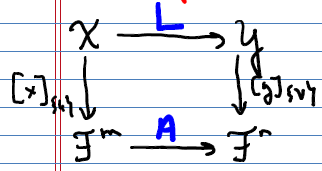
\includegraphics[width=0.42\columnwidth]{Chap02/DiagramChasingMatrixRep.png}}%
\hspace{5pt}%
\subfloat[]{%
	\centering
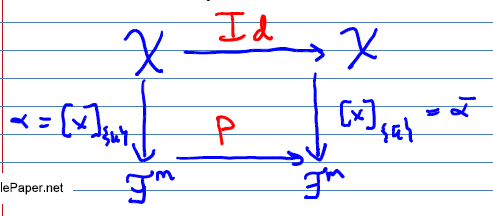
\includegraphics[width=0.52\columnwidth]{Chap02/DiagramChasingChangeOfBasis.png}}%
    \caption[]{Diagram chasing. Commuting diagrams used to illustrate the matrix representation of a linear operator and the change of basis matrix. When $\mathcal{X}=\mathcal{Y}$ and $\mathcal{L}=Id$, they become one and the same. Hence, there is really only one idea to remember.}
    \label{fig:DiagramChasing}
\end{figure} 

\vspace*{.2in}

\begin{example}
Let $\left(\mathcal{X},\mathcal{F}\right)=\left({\mathbb R}^{2},{\mathbb R}\right)$,
and define $L:{\mathbb R}^{2}\rightarrow{\mathbb R}^{2}$ by $L\left(e_{1}\right)=3e_{1}+4e_{2}$,
$L\left(e_{2}\right)=-e_{1}+6e_{2}$, where $e_{1}=\begin{bmatrix}1\\
0
\end{bmatrix}$ and $e_{2}=\begin{bmatrix}0\\
1
\end{bmatrix}$ are the canonical basis elements.
\begin{enumerate}
            \renewcommand{\labelenumi}{(\alph{enumi})}
        \setlength{\itemsep}{.1cm}
\item What is the matrix representation of $L$ with respect to $\left\{ e_{1},e_{2}\right\} $?
\item What is the matrix representation of $L$ with respect to $\left\{ v^{1},v^{2}\right\} $
where $v^{1}=e_{1}+e_{2}$, $v^{2}=3e_{1}-4e_{2}$?
\end{enumerate}
    
    \end{example}

\textbf{Solution:}~\begin{enumerate}
            \renewcommand{\labelenumi}{(\alph{enumi})}
        \setlength{\itemsep}{.1cm}
\item Let $A=$matrix representation of $L$. Then the $i^{th}$ column
of $A=\left[L\left(e_{i}\right)\right]_{\left\{ e_{1},e_{2}\right\} }$.
Hence,
\begin{align*}
\left[L\left(e_{1}\right)\right]_{\left\{ e_{1},e_{2}\right\} }&=\begin{bmatrix}3\\
4
\end{bmatrix} \\
\left[L\left(e_{2}\right)\right]_{\left\{ e_{1},e_{2}\right\} }&=\begin{bmatrix}-1\\
~~6
\end{bmatrix} \\
\implies A&=\begin{bmatrix}3 & -1\\
4 &~ ~6
\end{bmatrix}.
\end{align*}

\item Let $P$ be the change of coordinates from $\left\{ e_{1},e_{2}\right\} $
to $\left\{ v^{1},v^{2}\right\} $, and $\overline{P}$ be the change of
coordinates from $\left\{ v^{1},v^{2}\right\} $ to $\left\{ e_{1},e_{2}\right\} $.
Note that the $i^{th}$ column of $\overline{P}$ is just the representation
of $v^{i}$ in $\left\{ e_{1},e_{2}\right\} $. That is,
\[\overline{P}=\begin{bmatrix}1 & 3\\
1 & -4
\end{bmatrix}.\]
Recall that $\overline{P}=P^{-1}$, so
\[P=\left(\overline{P}\right)^{-1}=\frac{-1}{7}\begin{bmatrix}-4 & -3\\
-1 & 1
\end{bmatrix}=\frac{1}{7}\begin{bmatrix}4 & 3\\
1 & -1
\end{bmatrix}.\]
Therefore, if $\overline{A}$ is the representation of $L$ in $\left\{ v^{1},v^{2}\right\} $,
then
\[\overline{A}=PAP^{-1}=\frac{1}{7}\begin{bmatrix}4 & 3\\
1 & -1
\end{bmatrix}\begin{bmatrix}3 & -1\\
4 & 6
\end{bmatrix}\begin{bmatrix}1 & 3\\
1 & -4
\end{bmatrix}=\frac{1}{7}\begin{bmatrix}-38 & 16\\
-8 & 25
\end{bmatrix}.\]\\
\textbf{Note:} $\overline{P}$ was readily available, not $P$,
as you may have guessed!! Just to check, let's do the same thing the ``long way'':\\
\begin{align*}
L\left(v^{1}\right) & =L\left(e_{1}+e_{2}\right)\\
 & =L\left(e_{1}\right)+L\left(e_{2}\right)\\
 & =\left(3e_{1}+4e_{2}\right)+\left(-e_{1}+6e_{2}\right)\\
 & =2e_{1}+10e_{2}\\
L\left(v^{2}\right) & =L\left(3e_{1}-4e_{2}\right)\\
 & =3L\left(e_{1}\right)-4L\left(e_{2}\right)\\
 & =3\left(3e_{1}+4e_{2}\right)-4\left(-e_{1}+6e_{2}\right)\\
 & 13e_{1}-12e_{2}
\end{align*}
$\left[L\left(v^{1}\right)\right]_{\left\{ v^{1},v^{2}\right\} }=?$
To find it, write
\begin{align*}
\begin{bmatrix}2\\
10
\end{bmatrix} & =\overline{a}_{11}\underbrace{\begin{bmatrix}1\\
1
\end{bmatrix}}_{v^{1}}+\overline{a}_{21}\underbrace{\begin{bmatrix}3\\
-4
\end{bmatrix}}_{v^{2}}=\begin{bmatrix}1 & 3\\
1 & -4
\end{bmatrix}\begin{bmatrix}\overline{a}_{11}\\
\overline{a}_{12}
\end{bmatrix}\\
\implies & \begin{bmatrix}\overline{a}_{11}\\
\overline{a}_{12}
\end{bmatrix}=\frac{1}{7}\begin{bmatrix}38\\
-18
\end{bmatrix}
\end{align*}
Similarly
\begin{align*}
\begin{bmatrix}13\\
-12
\end{bmatrix} & =\overline{a}_{12}\begin{bmatrix}1\\
1
\end{bmatrix}+\overline{a}_{22}\begin{bmatrix}3\\
-4
\end{bmatrix}\\
\implies & \begin{bmatrix}\overline{a}_{12}\\
\overline{a}_{22}
\end{bmatrix}=\frac{1}{7}\begin{bmatrix}16\\
25
\end{bmatrix}
\end{align*}
and hence
$$ \overline{A}  =\frac{1}{7}\begin{bmatrix}38 & 16\\
-8 & 25
\end{bmatrix}. $$
\end{enumerate}

\Qed

\section{Eigenvalues, Eigenvectors, and Diagonalization}

\begin{definition}
Let $A$ be an $n\times n$ matrix with complex coefficients. A scalar $\lambda \in \mathbb{C} $ is an \textbf{eigenvalue} (e-value) of $A$, if there exists a non-zero vector $v \in \mathbb{C}^{n}$ such that $Av=\lambda v$. Any such vector $v$ is called an \textbf{eigenvector} (e-vector) associated with $\lambda$. 
\end{definition}

Eigenvectors are not unique because if $Av=\lambda v$, then for all $\alpha \neq 0$, $A(\alpha v)=\lambda (\alpha v)$, and thus $\alpha v$ is also an e-vector. To find eigenvalues, we need to know conditions under which $\exists v\neq0$ such that $Av=\lambda v$.
    \begin{equation*}
     \exists v\neq 0 \text{ s.t. }   Av=\lambda v \iff  \exists v\neq 0 \text{ s.t. } (\lambda I-A)v=0\iff \textnormal{det}(\lambda I-A)=0
    \end{equation*}
    
    \vspace*{.2cm}

\begin{example} Find the e-values and e-vectors for $A=\left[\begin{array}{rr}
    0 & 1\\
    -1 & 0
    \end{array}\right]$.
    \end{example} 
    
\textbf{Solution:}  $A=\left[\begin{array}{rr}
    0 & 1\\
    -1 & 0
    \end{array}\right] \implies \det(\lambda I-A)=\lambda^2+1=0$. Therefore, the eigenvalues are $\lambda_{1}=j,\lambda_{2}=-j$. To find eigenvectors, we need to solve $(A-\lambda_{i}I)v^{i}=0$. The eigenvectors are 
    $$v^{1}=\left[\begin{array}{c}
        1\\
        j
    \end{array}\right],v^{2}=\left[\begin{array}{c}
        1\\
        -j
    \end{array}\right].$$
Note that both eigenvalues and eigenvectors are complex conjugate pairs. 
\Qed




\begin{definition}
$\Delta (\lambda) := \det(\lambda I - A) $ is called the \textbf{characteristic polynomial}. $ \Delta (\lambda) = 0$ is called the \textbf{characteristic equation}. By the Fundamental Theorem of Algebra, $\Delta (\lambda)$ can be factored as
$$ \Delta (\lambda) = (\lambda - \lambda_1)^{m_1}(\lambda - \lambda_2)^{m_2}\dotsb(\lambda - \lambda_p)^{m_p} $$
where $\lambda_1, \dotsb, \lambda_p$ are the distinct eigenvalues (roots), $m_i$ is the \textbf{algebraic multiplicity} of $\lambda_i$, and  $m_1 + m_2 + \cdots + m_p = n.$ The \textbf{geometric multiplicity} of $\lambda i$ is defined as $\eta_i:= \dim \nullspace(A - \lambda_iI)$.

\end{definition}



\begin{thm}
Let $A$ be an $n \times n$ matrix with coefficients in $\real$ or $\mathbb{C}$. If the e-values $\{ \lambda_1,\ldots, \lambda_n \}$ are distinct, that is, $\lambda_i \neq \lambda_j $ for all $1 \le i \neq j \le n$, then the e-vectors $\{ v^1,\ldots,v^n \}$ are linearly independent in ($\mathbb{C}^n$,$\mathbb{C}$).
\end{thm} 

\begin{rem}
Restatement of the theorem: If the e-values $\{ \lambda_1,  \ldots,\lambda_n \}$ are distinct then $\{ v^1,  \ldots,v^n \}$ is a basis for ($\mathbb{C}^n$,$\mathbb{C}$).
\end{rem}

\textbf{Proof:}~We prove the contrapositive: if $\{ v^1,  \ldots,v^n \}$ is linearly dependent then there is a repeated e-value ($\lambda_i = \lambda_j$ for some $ i \neq j$). \\

$\{ v^1,  \ldots,v^n \}$ linearly dependent $\implies \exists$  $\alpha_1,  \ldots,\alpha_n \in \mathbb{C}$, not all zero, such that 
\begin{equation}
\label{eq:EvectorDependent}
     \alpha_1 v^1 + \dotsb + \alpha_n v^n = 0.
\end{equation}
   Without loss of generality, we can suppose $\alpha_1 \neq 0$. (that is, we can always reorder of e-values and e-vectors so that the first coefficient $\alpha_1$ is nonzero).\\
   
For all $1 \le i \le n$ and $1 \le j \le n$, because $v^i$ is an e-vector,
$$(A - \lambda_j I)v^i = A v^i - \lambda_j v^i = \lambda_i v^i - \lambda_j v^i = (\lambda_i - \lambda_j) v^i.$$

Using this fact, it is an easy exercise to show 
\begin{equation}
\label{eq:ProductMatrices}
(A - \lambda_2 I)(A - \lambda_3 I)\dotsb(A - \lambda_n I)v^i = (\lambda_i - \lambda_2)(\lambda_i - \lambda_3)\dotsb(\lambda_i - \lambda_n)v^i, \text{ for  } 1 \leq i \leq n.
\end{equation}
Plugging in now for $i$ yields,\\

   for $i = 1$ $$ (A - \lambda_2 I)(A - \lambda_3 I)\dotsb(A - \lambda_n I)v^1 = (\lambda_1 - \lambda_2)(\lambda_1 - \lambda_3)\dotsb(\lambda_1 - \lambda_n)v^1; \hspace*{4.1cm}$$
    for $i = 2$ $$(A - \lambda_2 I)(A - \lambda_3 I)\dotsb(A - \lambda_n I)v^2= (\lambda_2 - \lambda_2)(\lambda_2 - \lambda_3)\dotsb(\lambda_2 - \lambda_n)v^2 = 0 \text{ because } (\lambda_2 - \lambda_2)=0;$$
    $$ \vdots$$
for $i = n$ $$ (A - \lambda_2 I)(A - \lambda_3 I)\dotsb(A - \lambda_n I)v^n = (\lambda_n - \lambda_2)(\lambda_n - \lambda_3)\dotsb(\lambda_n - \lambda_n)v^2 = 0 \text{ because } (\lambda_n - \lambda_n)=0. $$



    Combining the above with \eqref{eq:EvectorDependent}, we obtain
    \begin{align*}
        0 &= (A - \lambda_2 I)(A - \lambda_3 I)\dotsb(A - \lambda_n I)(\alpha_1 v^1 + \dotsb + \alpha_n v^n)\\
        & = \alpha_1 (\lambda_1 - \lambda_2)(\lambda_1 - \lambda_3)\dotsb(\lambda_1 - \lambda_n)v^1
    \end{align*}

    We know $\alpha_1 \neq 0$, as stated above, and $v^1 \neq 0$, by definition of e-vectors. Therefore, 
    $$0 = (\lambda_1 - \lambda_2)(\lambda_1 - \lambda_3)\dotsb(\lambda_1 - \lambda_n),$$
    and hence, at least one of the terms $(\lambda_1-\lambda_k)$, $2 \le k \le n$ must be zero. Therefore, there is a repeated e-value $\lambda_1 = \lambda_k $ for some $2 \leq k \leq n$. 
    \Qed



\vspace*{.2cm}

\section{A Few Additional Properties of Matrices}

\vspace*{.2cm}

\begin{definition}
Two $n \times n$ matrices $A$ and $B$ are \textbf{similar} if there exists an invertible $n \times n$ matrix $P$ such that $B=P \cdot A \cdot P^{-1}$. $P$ is called a \textbf{similarity} matrix. 
\end{definition}

\begin{definition}
An $n \times n$ matrix $A$ is said to have a \textbf{full set of e-vectors} if there exists a basis $\{ v^1, v^2, \ldots, v^n\}$ of $(\cp^n, \cp)$ such $A v^i = \lambda_i v^i$, $1 \le i \le n$.
\end{definition}

\begin{thm}
\label{thm:SimilarDiagnonalMatrix}
An $n \times n$ matrix $A$ has a full set of e-vectors if, and only if, it is similar to a diagonal matrix. And when this happens, the entries on the diagonal matrix are e-values of $A$.
\end{thm} 

\textbf{Proof:} We assume that $\{ v^1, \ldots, v^n \}$ is a basis for $(\cp^n, \cp)$ and that for $1 \le i \le n$, $A v^i = \lambda_i v^i$. Define two $n \times n$ matrices
\begin{align*}
    M &:= \left[ \begin{array}{cccc} v^1 & v^2 & \cdots & v^n \end{array} \right] \\
    \Lambda &:= {\rm diag}(\lambda_1, \lambda_2, \ldots, \lambda_n).
\end{align*}
Then 
\begin{align*}
   A \cdot M &:= \left[ \begin{array}{cccc} A v^1 & A v^2 & \cdots & A v^n \end{array} \right] \\
   &=\left[ \begin{array}{cccc} \lambda_1 v^1 & \lambda_2 v^2 & \cdots & \lambda_n v^n \end{array} \right] \\
  &= M \cdot \Lambda.
\end{align*}
 
 We'll leave as an Exercise, 
 $$ M  \alpha = \left[ \begin{array}{cccc} v^1 & v^2 & \cdots & v^n \end{array} \right]  \begin{bmatrix}\alpha_{1}\\
            \alpha_{2}\\
            \vdots\\
            \alpha_{n}
        \end{bmatrix} = \alpha_1 v^2 + \alpha_2 v^2 + \cdots + \alpha_n v^n,$$
        and hence $M$ is invertible if, and only if, $\{ v^1, \ldots, v^n \}$ is linearly independent. Therefore we have 
        $$A = M \Lambda M^{-1} \text{ and } \Lambda = M^{-1} A M, $$
        proving that  $\{ v^1, \ldots, v^n \}$ is a basis implies $A$ is similar to a diagonal matrix. \\
        
        The other direction is straightforward and left to the reader. You need to recognize the columns of the ``similarity matrix'' as being e-vectors of $A$.
\Qed

\begin{fact}
If $A$ and $B$ are similar, they have the same e-values. Moreover, the e-values have the same algebraic and geometric multiplicities. 
\end{fact} 



\begin{definition}
 Let $A$ be an $n \times m$ matrix with coefficients in $\real$ or  $\cp$. The \textbf{rank} of $A$ is equal to the number of linearly independent columns. 
\end{definition}

\begin{fact}
If $M$ is square, then $\rank(M)$ equals the number of non-zero e-values.
\end{fact}

\begin{fact}
\label{fact:rankAAtranspose}
For an $n \times m$ real matrix $A$, $\rank(A) = \rank(A^\top A) = \rank(AA^\top) = \rank(A^\top)$. Hence, $A^\top A$ and $AA^\top$ have the same number of non-zero e-values. For a proof, see Chapter 10 of the ROB 101 textbook and see Lemma~\ref{lem:EigenStuffAAtranspose} below.
\end{fact} 




\begin{cor}\mbox{ }
\begin{itemize}
    \item $\#$ of linearly independent rows  = $\#$ of linearly independent columns.
    \item $\rank(A) \le \min(n, m)$
\end{itemize}
\end{cor}

\begin{lem}
\label{lem:EigenStuffAAtranspose}
Suppose that $A$ is a real $n \times m$ matrix. Then, 
\begin{itemize}
    \item If $\lambda$ is a non-zero e-value of $\left(A^\top A \right)$ with e-vector $v$, then $\lambda$ is also an e-value of $\left(A A^\top \right)$ with e-vector $A v$.
    \item If $\lambda$ is a non-zero e-value of $\left(A A^\top \right)$ with e-vector $v$, then $\lambda$ is also an e-value of $\left( A^\top A \right)$ with e-vector $A^\top  v$.
\end{itemize}
\end{lem}

\textbf{Proof:} We only prove the first statement. Suppose that $\left(A^\top A \right)v = \lambda v$ and both $\lambda$ and $v$ are non-zero. Then $Av \neq 0$. Next, we form 
$$\left(A A^\top \right) \left(A v \right)= A  \left( A^\top A\right)  v = A \left(\lambda v\right) = \lambda \left(Av\right),$$ 
and thus $\lambda$ is an e-value of $\left(A A^\top \right)$ with e-vector $Av$.

\Qed

\begin{cor} $A A^\top$ and $A^\top A$ have the same non-zero e-values. Because they have different sizes, they may have different number of zero e-values. 
\end{cor}

\begin{definition}(\textbf{Trace of a Matrix}) Let $C$ be an $n \times n$ matrix. Then $\tr(C):=\sum_{i-1}^n C_{ii}.$
\end{definition}

\begin{exercise} Suppose that $A$ is $n \times m$ and $B$ is $m \times n$. Then
$$\tr(A\cdot B) = \tr(B \cdot A). $$

\end{exercise}

 
\begin{fact}
\label{fact:MatMultiplyAlternative}
\textbf{(A lesser known way doing matrix multiplication, the outer product formula.)}  Suppose that $A$ is $n \times k$ and $B$ is $k \times m$ so that the two matrices are compatible for matrix multiplication. Then 
$$A\cdot B = \sum_{i=1}^{k} a_i^{\rm col} \cdot b_i^{\rm row},  $$
the ``sum of the columns of $A$ multiplied by the rows of $B$''. A more precise way to say it would be ``the sum over $i$ of the $i$-th column of $A$ times the $i$-th row of $B$.'' 
\end{fact}

\textbf{Why:} To see why this is true, let's first consider two $2 \times 2$ matrices $A$ and $B$, where
$$A= \left[\begin{array}{cc} a_{11}& a_{12} \\ a_{21} & a_{22}\end{array}\right]
\text{ and } B= \left[\begin{array}{cc} b_{11}& b_{12} \\ b_{21} & b_{22}\end{array}\right]
.$$
Then, using the standard rows of $A$ times the columns of $B$ formulation of matrix multiplication yields
$$
\begin{aligned}
 A \cdot B := &
\left[\begin{array}{cc}  a_1^{\rm row} \cdot b_1^{\rm col} & a_1^{\rm row} \cdot b_2^{\rm col}  \medskip  \\
a_2^{\rm row} \cdot b_1^{\rm col} & a_2^{\rm row} \cdot b_2^{\rm col}
\end{array}\right] \\ 
=& \left[\begin{array}{cc}  a_{11} b_{11} + a_{12}b_{21} & a_{11} b_{12} + a_{12}b_{22} \\
a_{21} b_{11} + a_{22}b_{21} & a_{21} b_{12} + a_{22}b_{22}
\end{array}\right]\bigskip  \text{(next, we take the sum outside the matrix)}\\
=& \left[\begin{array}{cc}  a_{11} b_{11}  & a_{11} b_{12} \\
a_{21} b_{11}  & a_{21} b_{12} 
\end{array}\right] + \left[\begin{array}{cc}  a_{12} b_{21}  & a_{12} b_{22} \\
a_{22} b_{21}  & a_{22} b_{22} 
\end{array}\right] \bigskip  \text{(next, we recognize each term)}\\
=& \left[\begin{array}{c} a_{11}\\ a_{21} \end{array}\right] \cdot 
 \left[\begin{array}{cc} b_{11}& b_{12} \end{array}\right] + 
 \left[\begin{array}{c} a_{12}\\ a_{22} \end{array}\right] \cdot 
 \left[\begin{array}{cc} b_{21}& b_{22} \end{array}\right]\\
=& a^{\rm col}_1 \cdot b^{\rm row}_1 + a^{\rm col}_2 \cdot b^{\rm row}_2
\end{aligned}
$$

In a similar manner, we can treat the general case,
\begin{equation}
\begin{aligned}
   A \cdot B:=&  \left[\begin{array}{c}\boxed{a_{11}~~ a_{12}~~ \cdots~~ a_{1k}}  \medskip \\
\boxed{a_{21}~~ a_{22}~~ \cdots~~ a_{2k}} \\
\vdots \\
\boxed{a_{n1}~~ a_{n2}~~ \cdots~~ a_{nk}}\end{array}\right] \cdot 
\left[ \boxed{\begin{array}{c} b_{11} \\ b_{21}\\ \vdots \\ b_{k1}\end{array} }~~~
\boxed{\begin{array}{c} b_{12} \\ b_{22}\\ \vdots \\ b_{k2}\end{array} }~~~\cdots~~~
\boxed{\begin{array}{c} b_{1m} \\ b_{2m}\\ \vdots \\ b_{km}\end{array} }\right] \\
=&
%
\left[\begin{array}{cccc}  \sum\limits_{i=1}^k a_{1i}b_{i1} & \sum\limits_{i=1}^k a_{1i}b_{i2} & \cdots & \sum\limits_{i=1}^k a_{1i}b_{im}  \medskip \\
 \sum\limits_{i=1}^k a_{2i}b_{i1} & \sum\limits_{i=1}^k a_{2i}b_{i2} & \cdots & \sum\limits_{i=1}^k a_{2i}b_{im} \\
\vdots & \vdots & \ddots & \vdots \\
 \sum\limits_{i=1}^k a_{ni}b_{i1} & \sum\limits_{i=1}^k a_{ni}b_{i2} & \cdots & \sum\limits_{i=1}^k a_{ni}b_{im} \\
\end{array}\right] \text{ (next, we pull the sum outside the matrix)}\\
=& \sum\limits_{i=1}^k
\left[\begin{array}{cccc}   a_{1i}b_{i1} &a_{1i}b_{i2} & \cdots &  a_{1i}b_{im}  \medskip \\
     a_{2i}b_{i1} & a_{2i}b_{i2} & \cdots &  a_{2i}b_{im} \\
\vdots & \vdots & \ddots & \vdots \\
  a_{ni}b_{i1} & a_{ni}b_{i2} & \cdots &  a_{ni}b_{im} \\
\end{array}\right] \text{(next, we recognize what this is)}\\
=& \sum_{i=1}^{k} a_i^{\rm col} \cdot b_i^{\rm row} \\
=&
\left[ \boxed{\begin{array}{c} a_{11} \\ a_{21}\\ \vdots \\ a_{n1}\end{array} }~~~
\boxed{\begin{array}{c} a_{12} \\ a_{22}\\ \vdots \\ a_{n2}\end{array} }~~~\cdots~~~
\boxed{\begin{array}{c} a_{1k} \\ a_{2k}\\ \vdots \\ a_{nk}\end{array} }\right] \cdot  \left[\begin{array}{c}\boxed{b_{11}~~ b_{12}~~ \cdots~~ b_{1m}}  \medskip \\
\boxed{b_{21}~~ b_{22}~~ \cdots~~ b_{2m}} \\
\vdots \\
\boxed{b_{k1}~~ b_{k2}~~ \cdots~~ b_{km}}\end{array}\right]. \
\end{aligned}
\end{equation}
\Qed


\begin{fact} \textbf{(Matrix Inversion Lemma)} Suppose that $A$, $B$, $C$ and $D$ are compatible\footnote{The sizes are such the matrix products and sum in $A+BCD$ make sense.} matrices. If $A$, $C$, and  $(C^{-1}+D A^{-1}B)$ are each square and invertible, then  $A+BCD$ is invertible and
    $$ (A + BCD)^{-1} = A^{-1} - A^{-1}B(C^{-1} + DA^{-1}B)^{-1}DA^{-1}$$
\end{fact}

\begin{rem} In many important applications, the inverse of $A$ may be already known or easy to compute. Here is a made up example, but it gets the point across: By hand, evaluate $ (A + BCD)^{-1}$ when
        $$A=\mathrm{diag}([1,~0.5, ~0.5,~1,~ 0.5]), ~ B=\begin{bmatrix} 1 \\ 0\\ 2\\ 0 \\3 \end{bmatrix}, C=0.2, D= B^\top $$
\end{rem}





\chapter{Abstract Inner Product Spaces for a Clear Vision of Deterministic Least Squares Problems}
\label{chap:IPSpacesandLeastSqaures}
\section*{Learning Objectives}

\begin{itemize}
\item Learn that a norm is a general means of measuring the length of a vector. 
\item Learn how the notions of an inner product and an inner product space generalize the dot product on $\real^n$ to a wide range of useful settings.
\item Apply the tools of inner product spaces to best approximation problems. 
\end{itemize}

\section*{Outcomes} 
\begin{itemize}
\item Norms and normed spaces as settings where best approximation problems can be posed.
\item Learn that orthogonality, the Pythagorean Theorem, and Gram-Schmidt work just as well in abstract inner product spaces as they do in $\real^n$.
\item The ``normal equations'' provide a systematic means to compute solutions to best approximation problems in any finite-dimensional inner product space.
\item While we are on the subject of ``orthogonality'', we'll dive into real symmetric matrices and see that their eigenvectors have the amazing property that they can be selected to form an orthonormal basis for $\real^n$.
\item We solve two very important least squares problems for overdetermined systems, underdetermined systems, and provide a recursive solution for the case of overdetermined systems. The latter is meant as a preview of the Kalman Filter (KF).
\end{itemize}

\newpage

\section{Preliminaries on Norms and Normed Spaces}
\label{sec:NormsDistance}


\begin{definition}
 Let $(\mathcal{X}, \mathcal{F})$ be a vector space where the field $\mathcal{F} $ is either $\real$ or $\cp$. A function $\| \cdot \|$: $\mathcal{X} \to\real  $ is a \textbf{norm} if it satisfies
 \begin{enumerate}
            \renewcommand{\labelenumi}{(\alph{enumi})}
        \setlength{\itemsep}{.1cm}
        \item $\| x \| \ge 0$, $\forall x \in \mathcal{X}$ and $\| x \| = 0 \iff \ x = 0$.
        \item Triangle inequality: $\| x+y \| \le \|x\| + \|y\|, \forall x, y \in \mathcal{X}$
        \item $\| \alpha x\| = |\alpha| \cdot \|x\|$, $\forall x\in \mathcal{X}, \alpha \in \mathcal{F}$,
            $
            \begin{cases}
                \textnormal{If } \alpha \in\real\textnormal{, } |\alpha| \textnormal{ means the absolute value}\\
                \textnormal{If } \alpha \in \mathbb{C}\textnormal{, } |\alpha| \textnormal{ means the magnitude}
            \end{cases}
            $.
    \end{enumerate}
     
\end{definition}


\begin{example} \mbox{ }
\begin{enumerate}
            \renewcommand{\labelenumi}{(\alph{enumi})}
        \setlength{\itemsep}{.1cm}
    \item $\mathcal{F} :=\real$ or $\mathbb{C}$, $\mathcal{X} := \mathcal{F}^n$.
	    \begin{itemize}
	        \item $\|x\|_2 := \left(\sum\limits_{i=1}^{n} |x_i|^2\right)^\frac{1}{2}$, Euclidean norm or 2-norm
	        \item $\|x\|_p := \left(\sum\limits_{i=1}^{n} |x_i|^p\right)^\frac{1}{p}, 1\le p < \infty$, p-norm
	        \item $\|x\|_\infty := \max\limits_{1 \le i \le n}|x_i|$, max-norm, sup-norm, $\infty$-norm
	    \end{itemize}
    \item $\mathcal{F} :=\real$, $\mathcal{D}\subset\real$, $\mathcal{D}:=[a, b]$, $a < b < \infty$, and $\mathcal{X} := \{f:\mathcal{D}\rightarrow\real\ |\ f \text{ is continuous} \}$.
        \begin{itemize}
            \item $\|f\|_2 := (\int_a^b \! |f(t)|^2 \, \mathrm{d}t)^\frac{1}{2}$
            \item $\|f\|_p := (\int_a^b \! |f(t)|^p \, \mathrm{d}t)^\frac{1}{p}$, $1 \le p <  \infty$
            \item $\|f\|_\infty := \max\limits_{a \le t \le b}|f(t)|$, which is also written $\|f\|_\infty := \sup \limits_{a \le t \le b} |f(t)|$
        \end{itemize}
\end{enumerate}
\end{example}


\begin{definition}
 $(\mathcal{X}, \mathcal{F}, \|\cdot\|)$ is called a \textbf{normed space}.
\end{definition} 


\begin{notvocab}
\textbf{(Notions of Distance and Best Approximation)} For $x, y \in \mathcal{X}$,
\begin{itemize}
    \item  $d(x, y) := \|x-y\|$ is called the \textbf{distance from} $x$ to $y$. We note that  $d(x, y) = d(y, x)$.
    \item  \textbf{Distance to a set:} Let $S\subset \mathcal{X}$ be a subset.
    \begin{equation*}
        d(x, S):= \inf \limits_{y\in S}\|x-y\|
    \end{equation*}
    \item  If $\exists x^\ast  \in S$ such that $d(x, S) = \|x-x^\ast \|$, then $x^\ast $ is called \textbf{a best approximation of $x$ by} \textbf{elements of $S$}.  We sometimes write $\widehat{x}$ for $x^\ast $ because we are really thinking of the solution as an approximation.
\end{itemize}

\end{notvocab}

\begin{question} \textbf{(Important questions for this chapter)}
\begin{enumerate}
         \renewcommand{\labelenumi}{(\alph{enumi})}
        \setlength{\itemsep}{.1cm}
    \item When does a best approximate $x^\ast $ exist?
    \item How to characterize (compute) $x^\ast $ such that $\|x-x^\ast \| = d(x, S)$, $x^\ast \in S$?
    \item If a solution exists, is it unique?
\end{enumerate}
\end{question}


\begin{notation} \textbf{(arg min)}
When $x^\ast $ exists and is unique, we write $x^\ast  := {\underset{y \in S}{\argmin}} \|x-y\|$ or  $\widehat{x} := {\underset{y \in S}{\argmin}} \|x-y\|$. It means that $x^\ast$ is the \textbf{argument of the minimum function that achieves the minimum value.}
\end{notation}

\begin{rem}  \mbox{ }
\begin{enumerate}
         \renewcommand{\labelenumi}{(\alph{enumi})}
        \setlength{\itemsep}{.1cm}
    \item $e:=x-y$ is the \textbf{error} when $x$ is approximated by $y \in S$.  
    \item $\underset{y \in S}{\inf}\|x-y\|$ is the smallest value that of the norm of the error that can be achieved over all elements $y\in S$. 
    \item When $\exists \widetilde{y} \in S$ such that $||x-\widetilde{y}|| =  \underset{y \in S}{\inf}  \|x-y\|$, we can write $||x-\widetilde{y}|| =  \underset{y \in S}{\min }\|x-y\|$. While it may seem natural to denote the best $y$ by $y^\ast$, we typically denote it by $x^\ast$ because we are trying to best approximate $x$ by elements of $S$.
    \item $x^\ast  := \underset{y \in S}{\argmin} \|x-y\|$ is the value of $y\in S$ that best achieves the approximation of $x$ in the sense of minimizing the norm.
    \item $x^\ast  := {\underset{y \in S}{\argmin}} \|x-y\|$ only makes sense when ${\underset{y \in S}{\operatorname{\inf}}} \|x-y\| = {\underset{y \in S}{\operatorname{\min}}} \|x-y\|$, that is, the infimum is actually achieved. 
    \item Furthermore, if you really want to be careful, you should also check that there is a unique minimum. Otherwise, the correct notation is $x^\ast  \in  {\underset{y \in S}{\argmin}} \|x-y\|$. In engineering publications, you rarely see this much care being taken. C'\'est la vie, baby !
\end{enumerate}

\end{rem}


\begin{figure}[htb!]%
	\centering{
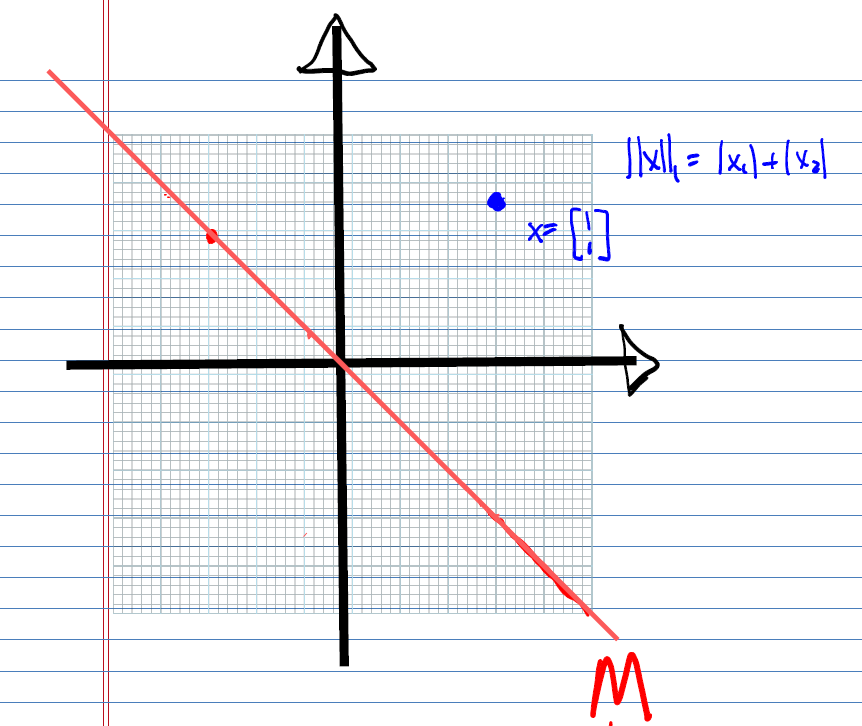
\includegraphics[width=0.7\columnwidth]{graphics/Chap03/NonUniqueMinimizingVector.png} }
    \caption[]{In HW, we'll introduce the concept of ``strict'' norms. The $|| \bullet ||_1$ is not strict and consequently, the minimum distance problem (or best approximation problem) does not have a unique answer. }
    \label{fig:NonUniqueMinimizingVector}
\end{figure} 

\begin{rem}
Figure~\ref{fig:NonUniqueMinimizingVector} shows an example having \textbf{nonunique solutions}. Indeed,  the set
$$S:= {\underset{y \in M}{\argmin}} \|x-y\|_1$$
contains an uncountable number of elements. Specifically, every element of
$$S=\left\{ \begin{bmatrix} x_1 \\ x_2 \end{bmatrix}~\big|~ x_2=-x_1, |x_1|\le 1 \right\} $$
is a minimizing vector for $x=[1~~~1]^\top$. That is, 
$$\forall~\widehat{x} \in S,~ ||x - \widehat{x}||_1 = 2 = \inf_{m \in M} ||x-m||_1.$$
To see this, you need to show that, $\forall~\widehat{x} \in S,$
\begin{align*}||x - \widehat{x}||_1 &= |1 - \hat{x}_1| + | 1 + \hat{x}_1|, ~-1 \le  \hat{x}_1 \le 1\\
& = (1 - \hat{x}_1)  +  ( 1 + \hat{x}_1) \\
&=2
\end{align*}
\end{rem}


\begin{exercise} Consider $(\real^n, \real)$ with the $p$-norm. Show that for all $x\in \real^n$, 
$$\lim_{p \to \infty}||x||_p= ||x||_{\rm max}. $$
\end{exercise}

\textbf{Hints:} (i) Prove the result when $||x||_{\rm max} =1$. (ii) When $x\neq 0$, consider $\bar{x} = x /||x||_{\rm max}$. (iii) For any non-negative real number $a$, $\lim_{p\to \infty} \sqrt[^p]{a} =1$.



\section{Inner Product Spaces}

\begin{recall}
For $z = \alpha + j\beta \, \in \mathbb{C}$, $\alpha, \beta \in\real$, we define $\mathrm{Re}\{z\}:=\alpha$ and  $\mathrm{Im}\{z\}:=\beta$. Note that $\mathrm{Im}\{z\}\in \real$. The complex conjugate of $z$ is $\overline{z} := \alpha -  j\beta$ and $|z| := \sqrt{\ z \cdot \overline{z}~ }= \sqrt{\alpha^2 + \beta^2}$.  Note that $z \in \real \iff (z = \overline{z}) \iff (\mathrm{Im}\{z\}=0)$.  For any complex number $z$, $\mathrm{Re}\{z\} \le |z|$. Finally, $ z = 0 \iff \overline{z} = 0 \iff |z|=0$.
\end{recall}

\begin{definition}
    Let $(\mathcal{X}, \mathbb{C})$ be a vector space. A function $\langle \cdot \, , \cdot \rangle: \mathcal{X} \times \mathcal{X} \rightarrow \mathbb{C}$
is an inner product if
    \begin{enumerate}
    \renewcommand{\labelenumi}{(\alph{enumi})}
        \setlength{\itemsep}{.1cm}
        \item $\langle a, b\rangle = \overline{\langle b, a\rangle}$.
        \item $\langle \alpha_1 x_1 + \alpha_2 x_2, y \rangle = \alpha_1 \langle x_1, y \rangle + \alpha_2 \langle x_2, y \rangle$, linear in the left argument. Some books place the linearity on the right side. 
        \item $\langle x, x \rangle \, \ge \, 0$ for any $x \in \mathcal{X}$, and $\langle x, x \rangle\,=\, 0$ $\iff$ $x = 0$. (See below: $\langle x, x \rangle$ is a real number and therefore it can be compared to 0.)
    \end{enumerate}
     
\end{definition}

\begin{rem} \mbox{ }
 \begin{enumerate}
        \item $\langle x, x \rangle\, =\, \overline{\langle x, x \rangle}$, by (a) and hence, $\langle x, x \rangle$ is always a real number.
        \item If the vector space is defined as $(\mathcal{X},\real)$, replace (a) with $(\text{a}^{'})$ $\langle a, b \rangle \, =\, \langle b, a \rangle$
        \item What about linear combinations on the right side? From (a) and (b)
        \begin{align*}
        \langle x, \beta_1 y_1 + \beta_2 y_2 \rangle &= \overline { \langle \beta_1 y_1 + \beta_2 y_2 ,  x\rangle }\\
        & =\overline {  \beta_1 \langle y_1 ,  x\rangle +  \beta_2  \langle y_2  ,  x\rangle }\\
        & =\overline{ \beta_1} ~~\overline{ \langle y_1 ,  x\rangle}  + \overline{ \beta_2}~~  \overline{ \langle y_2  ,  x\rangle }\\
         & =\overline{ \beta_1} ~\langle x, y_1 \rangle  + \overline{ \beta_2}  ~ \langle x,  y_2 \rangle 
        \end{align*}
        \item If the field is the real numbers, then the above reduces to $ \langle x, \beta_1 y_1 + \beta_2 y_2 \rangle = \beta_1 ~\langle x, y_1 \rangle  +  \beta_2  ~ \langle x,  y_2 \rangle  $
    \end{enumerate}

\end{rem}
   


\begin{example} Common inner products:
    \begin{enumerate}
        \renewcommand{\labelenumi}{(\alph{enumi})}
        \setlength{\itemsep}{.1cm}
        \item $(\mathbb{C}^n, \mathbb{C})$, $\langle x, y\rangle\, :=\, x^\top \overline{y}\, =\, \sum\limits_{i=1}^{n}x_i\overline{y_i}$.
        \item $(\real ^n,\real)$, $\langle x, y\rangle\, :=\, {x^\top }{y}\, =\, \sum\limits_{i=1}^{n}{x_i}{y_i}$.
        \item $\mathcal{F} =\real$, $\mathcal{X} = \{A\, |\, n\times m \,\, \text{real matrices} \}$, $\langle A, B\rangle\, :=\, \tr(AB^\top )\, = \, \tr(A^\top  B)$.
        \item $\mathcal{X} = \{ f: [a, b]\rightarrow\real , \text{$f$ continuous}\}$, $\mathcal{F} =\real$, $\langle f, g\rangle\, :=\,  \int_a^b \! f(t)g(t) \, \mathrm{d}t$.
    \end{enumerate}

\end{example}

\begin{thm}
    \textbf{(Cauchy-Schwarz Inequality)} Let $(\mathcal{X}, \mathcal{F}, \langle \cdot\,,\cdot \rangle)$ be an inner product space, with $\mathcal{F}$ either $\real $ or $\mathbb{C}$. Then, for all $x, y\in \mathcal{X}$
    \begin{equation*}
        |\langle x, y\rangle|\, \le\, {\langle x, x \rangle}^{1/2}\langle y, y \rangle ^{1/2}.
    \end{equation*}
\end{thm}

\textbf{Proof:} We will first do the proof for $\mathcal{F} =\real$.  We note that if $y = 0$, the result is clearly true. Hence, we assume $y \neq 0$ and let $\lambda \in\real$ be a scalar that is to be chosen. Then,
    \begin{align*}
        0\, & \le ||x - \lambda y||^2 \\
        &=  \langle x-\lambda y,\, x-\lambda y \rangle\\
        &=\langle x,\, x-\lambda y \rangle - \lambda\langle y,\, x-\lambda y\rangle\\
        &=\langle x, x\rangle - \lambda\langle x, y\rangle - \lambda\langle y, x\rangle +
        \lambda^2 \langle y, y\rangle \\
        &=\langle x, x\rangle - 2\lambda\langle x, y\rangle + \lambda^2\langle y,y\rangle.
    \end{align*}

We'll now make a choice for $\lambda$ that minimizes $\langle x, x\rangle - 2\lambda\langle x, y\rangle + \lambda^2\langle y,y\rangle$. Taking the derivative with respect to $\lambda$ and setting it equal to zero yields $\lambda = \langle x, y \rangle/\langle y, y \rangle$. In case you are curious whether this is a max or min, note that $\langle y, y \rangle >0$ because $y \neq 0$.\\

Substituting in this value for $\lambda$ gives
    \begin{align*}
        0& \le \min \limits_{\lambda \in \real}~~{\langle x-\lambda y, x-\lambda y\rangle} \\
        & = \left. \langle x- \lambda y, x- \lambda y \rangle \right|_{ \lambda = \langle x, y \rangle/ \langle y, y \rangle } \\
        &=\langle x,x\rangle - 2{|\langle x, y\rangle|}^2/\langle y,y \rangle + {|\langle x, y \rangle|}^2/{\langle y, y\rangle}\\
        &=\langle x,x\rangle - |\langle x,y\rangle|^2/\langle y, y\rangle \\
        & \Downarrow \\
      0  &\le  \langle x,x\rangle \cdot \langle y, y\rangle -|\langle x,y\rangle|^2
    \end{align*}
    Therefore, we can conclude that $|\langle x,y\rangle|^2\leq\langle x,x\rangle\langle y,y\rangle$ $\implies$ $|\langle x,y\rangle|\leq\langle x,x\rangle^{1/2}\langle y,y\rangle^{1/2}$ and the proof is done.\\

We quickly outline the steps for $\mathcal{F}=\cp$. Because the inner product of a vector with itself is always a non-negative real number, for all scalars $\lambda \in \cp$,
$$0 \le ~ \langle x-\lambda y, x-\lambda y \rangle   = \langle x,x \rangle   - \lambda \langle  y, x \rangle   - \overline{\lambda} \langle  x, y \rangle   + |\lambda|^2 \langle y,y \rangle  .$$
 For the particular choice $\lambda = \frac{\langle x, y \rangle  }{\langle y,y \rangle  }$, direct calculation shows
$$0 \le~ \langle x,x \rangle   - \frac{|\langle x,y \rangle  |^2}{\langle y,y \rangle  }, $$
which gives
$$|\langle x,y \rangle  | \le \sqrt{\langle x,x \rangle   \langle y,y \rangle  } = \langle x,x \rangle  ^{1/2} \cdot \langle y,y \rangle  ^{1/2},$$ 
and the proof is done. \\

\textbf{Note:} With the above choice of $\lambda$, we have 
$$\lambda \cdot \langle  y, x \rangle   = \frac{|\langle x,y \rangle  |^2}{\langle y,y \rangle  },~~  \overline{\lambda} \cdot \langle  x, y \rangle   =  \frac{|\langle x,y \rangle  |^2}{\langle y,y \rangle  }, \text{ and } |\lambda|^2 \cdot \langle y,y \rangle   =\frac{|\langle x,y \rangle  |^2}{\langle y,y \rangle  }. $$
    
    \Qed
    
\vspace*{.2cm}

\begin{cor}
Let $(\mathcal{X}, \mathcal{F}, \langle \cdot\,,\cdot \rangle)$ be an inner product space, with $\mathcal{F}$ either $\real $ or $\mathbb{C}$. Then, $$\|x\| :=  \langle x,x \rangle ^{1/2} = \sqrt{ \langle x,x \rangle }$$
is a \textbf{norm}.
\end{cor} 

\textbf{Proof:} As before,  for clarity of exposition, we first assume $\mathcal{F} =\real$. We will only check the triangle inequality $\|x+y\| \leq \|x\| +\|y\|$, which is equivalent to showing $ \|x+y\|^2 \leq \|x\|^2 + \|y\|^2 + 2\|x\| \cdot \|y\|$. The other parts are left as an exercise.

    \begin{align*}
               \|x+y\|^2 &:=  \langle x+y,x+y \rangle  \\
        &=  \langle x,x+y \rangle  +  \langle y, x+y \rangle  \\
        &=  \langle x,x \rangle  + \langle x,y \rangle  +  \langle y,x \rangle +  \langle y,y \rangle  \\
        &= \|x\|^2 + \|y\|^2 +2 \langle x,y \rangle  \\
        &\leq \|x\|^2 + \|y\|^2 + 2\left| \langle x,y \rangle \right| \\
        &\leq \|x\|^2 + \|y\|^2 + 2\|x\| \cdot \|y\|\, 
    \end{align*}
    where the last step uses the Cauchy-Schwarz inequality.  \\
    
    We'll now quickly do the changes required to handle $\mathcal{F} = \cp$. The triangle inequality is
$
	\| x + y \| \leqslant \| x \| + \| y \|,
$ which is equivalent to showing $
	\| x + y \|^2 \leqslant \| x \|^2 + 2 \| x \| \, \| y \| + \| y \|^2.
$
Brute force computation yields,
\begin{align*}
	\| x + y \|^2 &= \langle x+y,x+y \rangle   \\
	&= \langle x,x+y \rangle   + \langle y,x+y \rangle  \\
&= \overline{\langle x+y,x \rangle  } + \overline{\langle x+y,y \rangle  }\\
&= \overline{\langle x,x \rangle   + \langle y,x \rangle  } + \overline{\langle x,y \rangle   + \langle y,y \rangle  }\\
	&= \langle x,x \rangle   +  \langle x,y \rangle   +   \overline{\langle x,y \rangle  }+ \langle y,y \rangle   \\
	&= \| x \|^2 + \| y \|^2 + 2 \mathrm{Re}\{ \langle x,y \rangle  \}
\end{align*}
where $\mathrm{Re}\{ \langle x,y \rangle  \}$ denotes the real part of the complex number $\langle x,y \rangle  $. However, for any complex number $\alpha$, $\mathrm{Re}\{\alpha \} \le | \alpha|$, and thus we have
\begin{align*}
\| x + y \|^2 &= \| x \|^2 + \| y \|^2 + 2 \mathrm{Re}\{ \langle x,y \rangle  \} \\
	&\leqslant \| x \|^2 + \| y \|^2 +
		 2 |\langle x,y \rangle  | \\
	&\leqslant \| x \|^2 + \| y \|^2
		+ 2 \|x \| \|y\|,
\end{align*}
where the last inequality is from the Cauchy-Schwarz Inequality.
    
    
    \Qed
    
    \vspace*{.2cm}
    

\begin{definition}
    Orthogonal and orthonormal vectors.
\begin{enumerate}
        \renewcommand{\labelenumi}{(\alph{enumi})}
        \setlength{\itemsep}{.1cm}
    \item Two vectors $x$ and $y$ are \textbf{orthogonal} if $ \langle x,y \rangle =0$. \textbf{Notation:} $x \perp y$
    \item \textbf{A set of vectors $S$ is orthogonal} if $$\forall x \text{,} y \in S \text{,} x \neq y \implies \langle x,y \rangle =0 \mbox{ (i.e. $ x \perp y$)}$$
    \item If in addition, $\|x\|=1$ for all $x \in S$, then $S$ is an \textbf{orthonormal set}.
\end{enumerate}

\end{definition}


\begin{rem}
 For $x \neq 0, \frac{x}{\|x\|}$ has norm 1, because 
    $\left \lVert \frac{x}{\|x\|}\right\rVert = \left| \frac{1}{\|x\|}\right| \cdot \|x\|=\frac{1}{\|x\|}\cdot \|x\|=1$.
\end{rem}

 \begin{thm}
     \textbf{(Pythagorean Theorem)} If $x \perp y$, then
    $$\|x+y\|^2 = \|x\|^2+ \|y\|^2.$$\\
 \end{thm}

\textbf{Proof:} From the proof of the triangle inequality,
    \begin{align*}
        \|x+y\|^2 &= \|x\|^2+ \|y\|^2+2 \langle x,y \rangle.
    \end{align*}
    Once we note that $ \langle x,y \rangle = 0$  because $ x \perp y$, we are done. 
    
\Qed

 
 \section{Gram Schmidt Process}
 
\begin{prop}
 \textbf{(Recursion Step Gram Schmidt Process)} Let $({\cal X, F}, \langle \cdot, \cdot \rangle  )$ be  an inner product space, $\{ y^1, \cdots, y^k\}$ a linearly independent set, and 
$\{ v^1, \cdots, v^{k-1} \}$ an orthogonal set satisfying
  \begin{equation}
 \label{eq:gramSchmidtStepkminus1}
 \spanof{ v^1, \cdots, v^{k-1} } = \spanof{ y^1, \cdots, y^{k-1} } .
  \end{equation}
 Define
 \begin{equation}
 \label{eq:gramSchmidtRecursion}
	v^k = y^k - \sum_{j=1}^{k-1}
	\frac{\langle y^k,v^j \rangle  }{\| v^j \|^2} \cdot v^j		
\end{equation}
where $ \| v^j \|^2 = \langle v^j,v^j \rangle  $. Then, $\{ v^1, \cdots, v^{k} \}$ is orthogonal and
 \begin{equation}
 \label{eq:gram_schmidt}
\spanof{ v^1, \cdots, v^{k} } = \spanof{y^1, \cdots, y^{k}}.
 \end{equation}

\end{prop}

\textbf{Proof:} We first note that from \eqref{eq:gramSchmidtStepkminus1}, $v^i \neq 0$  for $1 \le i \le k-1$. Next, the orthogonality of $\{ v^1, \cdots, v^{k} \}$ is essentially by construction. To see this, we write
 $$v^k = y^k - \sum_{i=1}^{k-1} a_{ki}v^i	 $$
 and then check that $\langle v^k,v^j \rangle  =0$ for $1 \le j \le  k-1$  if, and only if,
 $$ a_{kj}=	\frac{\langle y^k,v^j \rangle  }{\| v^j \|^2} .$$
 Indeed,  
 $$ \langle  v^i, v^j  \rangle   = \begin{cases}
 0 & j \neq i, 1 \le i,j \le k-1 \\
|| v^i|| ^2 & i = j,
 \end{cases} $$
and hence 
$$0 = \langle v^k, v^j \rangle    = \langle y^k, v^j \rangle   - \sum_{i=1}^{k-1} a_{ki} \langle v^i, v^j \rangle   = \langle y^k, v^j \rangle   -  a_{kj} \langle v^j, v^j \rangle  	=  \langle y^k, v^j \rangle   -  a_{kj} ||v^j||^2. $$ 

 We next show that $y^k \in \spanof{ v^1, \cdots, v^k }$ and $v^k \in \spanof{ y^1, \cdots, y^k }$.\\

From \eqref{eq:gramSchmidtRecursion},
\[
	y^k = v^k + \sum_{j=1}^{k-1}
	\frac{\langle y^k,v^j \rangle  }{\| v^j \|^2} \cdot v^j  \implies 
	y^k \in
		\spanof{ v^1, \cdots, v^k }.
\]
Left to show: $v^k \in \spanof{ y^1, \cdots, y^k }$. By hypothesis,
\[
	v^j \in \spanof{ y^1, \cdots, y^{k-1} }
		\mbox{ for all } 1 \leqslant j \leqslant k-1,
\]
so
\[
	\sum_{j=1}^{k-1}
	\left( \frac{\langle v^j,y^k \rangle  }{\| v^j \|^2} \right) v^j \
		\in \ \spanof{ y^1, \cdots, y^{k-1} } \
		\subset \ \spanof{ y^1, \cdots, y^k }.
\]
Clearly, $y^k \in \spanof{ y^1, \cdots, y^k }$. Putting these two facts together, 
\[
 v^k = y^k - \sum_{j=1}^{k-1}
	\left( \frac{\langle v^j,y^k \rangle  }{\| v^j \|^2} \right) v^j \
		\in \ \spanof{ y^1, \cdots, y^k }
\]
because $\spanof{ y^1, \cdots, y^k }$ is a subspace. 
\Qed

\vspace*{.2cm}

\begin{definition}
\label{def:ClassicalGS}
The \textbf{Gram-Schmidt Process} consists of initialing \eqref{eq:gramSchmidtStepkminus1} with $v^1 = y^1$ and then applying \eqref{eq:gramSchmidtRecursion} recursively. When implementing the algorithm in code, it is quite easy to normalize the vectors as you go, as in the following pseudocode: 
\begin{lstlisting}[language=Julia,style=mystyle]
# Given {y1, ..., yn} linearly independent
# Produce {v1, ..., vn} orthonormal such that
# span{v1, ... vk} = span{y1, ..., yk}
v1 = y1
v1=v1/norm(v1)
for k = 2 : n
vk = yk
    for j = 1 : k - 1
        vk = vk - < yk, vj > 
    end
    vk = vk/norm(vk)
end
\end{lstlisting}
    
\end{definition} 
% \textbf{Output}
% \begin{verbatim}
% 1×5 Matrix{Float64}:
%  1.0  -2.0  4.0  8.1  1.41421
% \end{verbatim}

\begin{example} Given the following data in $(\real^3,\real)$, 
\begin{gather*}
	\{ y^1, y^2, y^3 \} = \left\{
		\left[ \begin{array}{c} 1 \\ 1 \\ 0 \end{array} \right],
		\left[ \begin{array}{c} 1 \\ 2 \\ 3 \end{array} \right],
		\left[ \begin{array}{c} 0 \\ 1 \\ 1 \end{array} \right]
		\right\},
\end{gather*}
and inner product $<p,q> := p^T q = \sum_{i=1}^3 p_i q_i$, apply Gram-Schmidt to produce an orthogonal basis. Normalize to produce an orthonormal basis.
\end{example}

\textbf{Solution:}
	\begin{align*}
		v^1 &= y^1 = \left[ \begin{array}{c} 1 \\ 1 \\ 0 \end{array} \right]\\
		\quad \| v^1 \|^2 &= (v^1)^T v^1 = 2 ;\\
		\\
		v^2	&= y^2 - \frac{<v^1,y^2>}{\| v^1 \|^2} v^1 \\
		&= \left[ \begin{array}{c} 1 \\ 2 \\ 3 \end{array} \right]
		- \underbrace{%
		   \left[ \begin{array}{ccc} 1 & 1 & 0 \end{array} \right]
		   \left[ \begin{array}{c} 1 \\ 2 \\ 3 \end{array} \right]%
		   }_{3}
		\frac{1}{2}
		   \left[ \begin{array}{c} 1 \\ 1 \\ 0 \end{array} \right]
		= \left[ \begin{array}{r}
			- \frac{1}{2} \medskip \\ \frac{1}{2} \medskip \\ 3
			\end{array} \right] \\
		\| v^2 \|^2 &= 9 \frac{1}{2} = \frac{19}{2} ;\\
		\\
		v^3	&= y^3 - \frac{<v^1,y^3>}{\| v^1 \|^2} v^1
			- \frac{<v^2,y^3>}{\| v^2 \|^2} v^2 \\
		&= \left[ \begin{array}{c} 0 \\ 1 \\ 1 \end{array} \right]
		- \underbrace{%
		   \left[ \begin{array}{ccc} 1 & 1 & 0 \end{array} \right]
		   \left[ \begin{array}{c} 0 \\ 1 \\ 1 \end{array} \right]%
		   }_{1}
		\frac{1}{2}
		   \left[ \begin{array}{c} 1 \\ 1 \\ 0 \end{array} \right]
		- \underbrace{%
		   \left[ \begin{array}{ccc}
			-\frac{1}{2} & \frac{1}{2} & 3 \end{array} \right]
		   \left[ \begin{array}{c} 0 \\ 1 \\ 1 \end{array} \right]%
		   }_{3\frac{1}{2}}
		\frac{1}{\frac{19}{2}}
		   \left[ \begin{array}{r}
			-\frac{1}{2} \medskip \\ \frac{1}{2} \medskip \\ 3 \end{array} \right] \\
		&= \left[ \begin{array}{c} 0 \\ 1 \\ 1 \end{array} \right]
		- \left[ \begin{array}{c}
			\frac{1}{2} \\ \frac{1}{2} \\ 0 \end{array} \right]
		- \left[ \begin{array}{r}
			-\frac{7}{38} \medskip \\ \frac{7}{38} \medskip \\ \frac{21}{19}
			\end{array} \right]
		= \left[ \begin{array}{r}
			-\frac{6}{19} \medskip \\ \frac{6}{19} \medskip \\ -\frac{2}{19}
			\end{array} \right].
	\end{align*}

\textbf{Normalize to obtain Orthonormal Basis:}often useful to do this, but never fun to do by hand.\\
	\begin{align*}
		\tilde{v}_1 &= \frac{v^1}{\| v^1 \|} = \left[ \begin{array}{c} \frac{1}{\sqrt{2}} \medskip \\ \frac{1}{\sqrt{2}} \medskip \\ 0 \end{array} \right]\\
		\tilde{v}_2 &= \frac{v^2}{\| v^2 \|} = \left[ \begin{array}{r} \frac{-1}{\sqrt{38}} \medskip \\ \frac{1}{\sqrt{38}} \medskip \\ 3\sqrt{\frac{2}{19}} \end{array} \right]\\
		\tilde{v}_3 &= \frac{v^3}{\| v^3 \|} = \frac{19}{\sqrt{76}} \left[ \begin{array}{r} -\frac{6}{19} \medskip \\ \frac{6}{19} \medskip \\ -\frac{2}{19}
			\end{array} \right]\\
	\end{align*}
\Qed

\begin{example} Given the real vector space $C[0,1] = \{ f:[0,1] \rightarrow \real \mid f~~\mbox{continuous} \}$, inner product $<f,g> := \int_0^1 f(\tau) g(\tau) d\tau$, and 
	$\{ y^1, y^2, y^3 \} = \{ 1, t, t^2 \}$, apply Gram-Schmidt to produce an orthogonal basis for $\spanof{ 1, t, t^2}$.

\end{example}

\textbf{Solution:}

	\begin{align*}
		v^1 &= y^1 = 1\\
		\qquad \| v^1 \|^2 &= \int_0^1 (1)^2 d\tau = 1 ;\\
		\\
		v^2	&= y^2 - \frac{<v^1,y^2>}{\| v^1 \|^2} v^1 \\
		&= t - \underbrace{%
			\int_0^1 1 \cdot \tau d\tau%
			}_{\frac{1}{2}} \cdot \frac{1}{1} \cdot 1
		= t - \frac{1}{2} \\
		\| v^2 \|^2 &= \int_0^1 (\tau - \frac{1}{2})^2 d\tau = \frac{1}{12} ;\\
		\\
		v^3	&= y^3 - \frac{<v^1,y^3>}{\| v^1 \|^2} v^1
		- \frac{<v^2,y^3>}{\| v^2 \|^2} v^2 \\
		&= t^2 - \underbrace{%
			\int_0^1 1 \cdot \tau^2 d\tau%
			}_{\frac{1}{3}} \cdot \frac{1}{1} \cdot 1
		- \underbrace{%
			\int_0^1 (\tau - \frac{1}{2}) \tau^2 d\tau%
			}_{\frac{1}{12}} \left( \frac{1}{\frac{1}{12}} \right)
				\Bigl( t - \frac{1}{2} \Bigr) \\
		&= t^2 - \frac{1}{3} - \Bigl( t - \frac{1}{2} \Bigr) \\
		&= t^2 - t + \frac{1}{6}.
	\end{align*}
	\Qed

\begin{example}
Doing inner products on $C[a,b]$ in MATLAB
% \begin{alltt}
% >> clear *
% >> syms t % declare to be a symbolic variable

% >> % INT(S,a,b) is the definite integral of S with respect to
%   % its symbolic variable from a to b.  a and b are each
%   % double or symbolic scalars.

% >> y1=1+0*t; % Otherwise MATLAB will not treat y1 as a 
%             %trivial function of the symbolic variable 
% >> y2=t;
% >> y3=t^2;

% % Start the G-S Procedure. Here we assume C[0,1], that is
% % C[a,b], with [a,b]=[0,1]

% >> v1=y1
% >> v2=y2-int(v1*y2,0,1)*v1/int(v1^2,0,1)
% >> v3=y3-int(v1*y3,0,1)*v1/int(v1^2,0,1)-
% int(v2*y3,0,1)*v2/int(v2^2,0,1)

% % Next, normalize to length one

% >> v1_tilde=v1/int(v1^2,0,1)^.5
% >> v2_tilde=simplify( v2/int(v2^2,0,1)^.5 )
% >> v3_tilde=simplyfy(v3/int(v3^2,0,1)^.5)
% \end{alltt}

\begin{lstlisting}[language=Julia,style=mystyle]
>> clear *
>> syms t % declare to be a symbolic variable

>> % INT(S,a,b) is the definite integral of S with respect to
   % its symbolic variable from a to b.  a and b are each
   % double or symbolic scalars.

>> y1=1+0*t; % Otherwise MATLAB will not treat y1 as a 
            %trivial function of the symbolic variable 
>> y2=t;
>> y3=t^2;

% Start the G-S Procedure. Here we assume C[0,1], that is
% C[a,b], with [a,b]=[0,1]

>> v1=y1
>> v2=y2-int(v1*y2,0,1)*v1/int(v1^2,0,1)
>> v3=y3-int(v1*y3,0,1)*v1/int(v1^2,0,1)-
int(v2*y3,0,1)*v2/int(v2^2,0,1)

% Next, normalize to length one

>> v1_tilde=v1/int(v1^2,0,1)^.5
>> v2_tilde=simplify( v2/int(v2^2,0,1)^.5 )
>> v3_tilde=simplyfy(v3/int(v3^2,0,1)^.5)
\end{lstlisting}
\textbf{Output} 
\begin{verbatim}
v1=1
v2=t-1/2
v3=t^2+1/6-t

v1_tilde=1
v2_tilde=(t-1/2)*12^(1/2)
v3_tilde=(6*t^2+1-6*t)*5^(1/2)
 \end{verbatim}
 
 \end{example}

\begin{rem}
\label{rem:ModifiedGramSchmidt} \textbf{(Round-off Errors Affect Classical Gram-Schmidt)}
The classical Gram-Schmidt Process in Definition~\ref{def:ClassicalGS} is straightforward to understand, which is why it is taught in courses. Unfortunately, it behaves poorly under the round-off error that occurs in digital computations! Here is a standard example:
    \begin{equation*}
        u_1=\left[\begin{matrix} 1 \\ \varepsilon \\ 0 \\ 0 \end{matrix}\right],
        u_2=\left[\begin{matrix} 1 \\ 0 \\ \varepsilon \\ 0 \end{matrix}\right],
        u_3=\left[\begin{matrix} 1 \\ 0 \\ 0 \\ \varepsilon \end{matrix}\right],
        \varepsilon>0
    \end{equation*}
Let $\{e_1,e_2,e_3,e_4\}$ be the standard basis vectors corresponding to the columns of the $4 \times 4$ identity matrix. We note that
    \begin{align*}
        u_2 &= u_1+\varepsilon(e_3-e_2)\\
        u_3 &= u_2+\varepsilon(e_4-e_3)
    \end{align*}
    and thus, for $\epsilon \neq 0,$
    \begin{align*}
        \spanof{u_1,u_2}&=\spanof{u_1,(e_3-e_2)}\\
        \spanof{u_1,u_2,u_3}&=\spanof{u_1,(e_3-e_2),(e_4-e_3)}
    \end{align*}
\end{rem}


\begin{example}
Hence, Gram-Schmidt applied to $\{u_1,u_2,u_3\}$ and $\{u_1,(e_3-e_2),(e_4-e_3)\}$ should ``theoretically'' produce the same orthonormal vectors. To check this, we go to MATLAB, and for $\varepsilon=0.1$, we do indeed get the same results. You can verify this yourself. However, with $\varepsilon=10^{-8}$,
\begin{align*}
    Q_1 &= \left[ \begin{array}{rrr}
  1.0000     &    0.0000     &  0.0000  \\
    0.0000 &  -0.7071  & -0.7071 \\
        0.0000  &   0.7071   &      0.0000  \\
        0.0000   &      0.0000  &  0.7071
    \end{array} \right] \\
    Q_2&=\left[ \begin{array}{rrr}
  1.0000     &    0.0000     &  0.0000  \\
    0.0000 &  -0.7071  & -0.4082 \\
        0.0000  &   0.7071   &      -0.4082  \\
        0.0000   &      0.0000  &  0.8165
    \end{array} \right] 
    \end{align*}
where $$Q_1=\begin{bmatrix} \frac{v_1}{\| v_1 \|} & \frac{v_2}{\| v_2 \|} & \frac{v_3}{\| v_3 \|}\end{bmatrix}$$
has been computed with Classical-Gram-Schmidt for $\{u_1,u_2,u_3\}$ while $$Q_2=\begin{bmatrix} \frac{v_1}{\| v_1 \|} & \frac{v_2}{\| v_2 \|} & \frac{v_3}{\| v_3 \|}\end{bmatrix}$$
has been computed with Classical-Gram-Schmidt for $\{u_1,(e_3-e_2),(e_4-e_3)\}$. Hence we do NOT obtain the same result!
\end{example}



\begin{definition} \textbf{(Modified Gram-Schmidt)} has better numerical performance\\
for $k=1:n$\\
        \indent\hspace{4ex}$v_k=u_k$~~~\%copy over the vectors\\
        end \bigskip\\
        for $k=1:n$\\
        \indent\hspace{4ex}$v_k=\frac{v_k}{\|v_k\|}$ \medskip\\
        \indent\hspace{4ex}for $j=(k+1):n$  \medskip\\
        \indent\hspace{8ex}$v_j=v_j-(v_j \bullet v_k)v_k$  ~~~\%Makes $v_j$ orthogonal to  $v_k$\\
        \indent\hspace{4ex}end\\
        end\\
        At \textbf{Step k=1}, $v_1$ is normalized to length one, and then $v_2, \ldots, v_n$ are redefined to be orthogonal to $v_1$. At \textbf{Step k=2:}  $v_2$ is normalized to length one, and then $v_3, \ldots, v_n$ are redefined to be orthogonal to $v_2$. We note that they were already orthogonal to $v_1$.  At \textbf{Step k:}  $v_k$ is normalized to length one, and then $v_{k+1}, \ldots, v_n$ are redefined to be orthogonal to $v_k$. We note that they were already orthogonal to $v_1, \ldots, v_{k-1}$.    
\end{definition}
 
        
 \begin{example}
Hence, if Modified Gram-Schmidt is so great, when applied to $\{u_1,u_2,u_3\}$ and $\{u_1,(e_3-e_2),(e_4-e_3)\}$, it should produce the same orthonormal vectors and it does! To check this, we go to MATLAB for $\varepsilon=10^{-8}$ and obtain
\begin{align*}
    Q_1 &= \left[ \begin{array}{rrr}
  1.0000     &    0.0000     &  0.0000  \\
    0.0000 &  -0.7071  & -0.7071 \\
        0.0000  &   0.7071   &      0.0000  \\
        0.0000   &      0.0000  &  0.7071
    \end{array} \right] \\
    Q_2&=\left[ \begin{array}{rrr}
  1.0000     &    0.0000     &  0.0000  \\
    0.0000 &  -0.7071  & -0.7071 \\
        0.0000  &   0.7071   &      0.0000  \\
        0.0000   &      0.0000  &  0.7071
    \end{array} \right]
    \end{align*}
where $Q_1$ and $Q_2$ are defined above. \textbf{When one is equipped with the right Algorithm, the world is truly a marvelous place.}
  
  \end{example}
  
  \begin{rem}
Just to be perfectly clear, with perfect arithmetic (no rounding errors), Classical Gram-Schmidt and Modified Gram-Schmidt are equivalent. 
  \end{rem}
 
 \section{Projection Theorem and the Normal Equations}
 
\begin{lem} (called the Pre-Projection Theorem in Luenberger)
\label{lem:PreProjThm}
Let $\mathcal{X}$ be a finite-dimensional (real) inner product space, $M$ be a subspace of $\mathcal{X}$, and $x$ be an arbitrary point in $\mathcal{X}$.
    \begin{enumerate}
            \renewcommand{\labelenumi}{(\alph{enumi})}
        \setlength{\itemsep}{.1cm}
        \item If $\exists m_0 \in M $ such that $\|x-m_0\| \leq \|x-m\| \ \ \forall m \in M$, then $m_0$ is unique.
        \item A necessary and sufficient condition for $m_0$ to be a minimizing vector in $M$ is that the vector $x-m_0$ is orthogonal to $M$.
    \end{enumerate}
        
\end{lem}

\textbf{Remarks:}
    \begin{enumerate}
        \item[(a')] If $\exists m_0 \in M$ such that $\|x-m_0\| = d(x,M) = \underset{m \in M}{\text{inf}} \|x-m\|$, then $m_0$ is unique. [equivalent to (a)]
        \item[(b')] $\|x-m_0\| = d(x,M) \iff x-m_0 \perp M$. [equivalent to (b)]
    \end{enumerate}

\textbf{Proof:} We break the proof up into a series of claims.

\begin{claim}
If $m_0 \in M$ satisfies $\|x-m_0\| = d(x,M)$, then $x-m_0 \perp M$. 
\end{claim}
    \emph{Proof:} (By contrapositive) Assume $x-m_0 \not\perp M$. We will produce $m_1 \in M$ such that $\|x-m_1\| <  \|x-m_0\|$. Indeed, suppose $x-m_0 \not\perp M$. Then, $\exists m \in M$ such that $ \langle x-m_0, m \rangle  \neq 0$. We know $m \neq 0$, and hence we define 
    \begin{itemize}
        \item $\tilde{m} = \frac{m}{\|m\|} \in M$; 
        \item $\delta := \langle x-m_0, \tilde{m} \rangle  \neq 0$; and
        \item $m_1 = m_0 + \delta \tilde{m} \implies m_1 \in M$.
    \end{itemize}
The intuition behind the definition of $m_1$ is that $x-m_1$ is ``closer'' to being perpendicular to $M$ than is $x - m_0$, and hence it should follow that $||x - m_1|| < ||x-m_0||$.  To prove the latter point, we do a few computations:
        \begin{align*}
            \|x-m_1\|^2 &= \|x-m_0-\delta \tilde{m}\|^2 \\
            &=  \langle x-m_0-\delta \tilde{m}, x-m_0-\delta \tilde{m} \rangle  \\
            &=  \langle x-m_0,x-m_0 \rangle  -\delta \underbrace{\langle x-m_0,\tilde{m} \rangle}_\delta -\delta \underbrace{\langle \tilde{m},x-m_0 \rangle}_\delta  +\delta^2 \underbrace{\langle \tilde{m},\tilde{m} \rangle}_{=1}  \\
            &= \|x-m_0\|^2 -\delta^2 \\
            &< \|x-m_0\|^2
        \end{align*}
    because $\delta^2 >0$.  Hence, $\|x-m_1\|^2 <  \|x-m_0\|^2$ and therefore, $\|x-m_0\| \neq \underset{m \in M}{\inf  \|x-m\|}:= d(x,M)$.  \hfill   $\square$ 
   
 

\begin{claim}
 If $x-m_0 \perp M$, then $\|x-m_0\| = d(x,M)$ and $m_0$ is unique. 
\end{claim}
\emph{Proof:} Recall the Pythagorean Theorem:
    \begin{equation*}
        \|x+y\|^2=\|x\|^2+\|y\|^2 \mbox{ when } x \perp y
    \end{equation*}
    Let $m \in M$ be arbitrary and suppose $x-m_0 \perp M$. Then  $x-m_0 \perp  m_0-m$, and thus
    \begin{align*}
        \|x-m\|^2 &= \|x-m_0+\underbrace{m_0-m}_{\in M}\|^2 \\
        &= \|x-m_0\|^2 + \|m_0 - m\|^2.
    \end{align*}
    It follows that
    $$\underset{m \in M}{\text{inf}} \|x-m\|^2=\underset{m \in M}{\inf~ }\left( \|x-m_0\|^2 + \|m_0 - m\|^2 \right) = 
     \|x-m_0\|^2 + \underset{m \in M}{\inf~ } \|m_0 - m\|^2 =\|x-m_0\|^2. $$ 
The unique minimizer is $m_0$ because $ \|m_0 - m\|^2 =0$  only for $m=m_0$. \hfill $\square$ \\

The two claims complete the proof. 

\Qed

\begin{definition}
Let $({\cal X, F},  \langle \cdot,\cdot \rangle )$ be an inner product space, and $S \subset {\cal X}$ a \emph{subset} (does not have to be a subspace). 
$$S^{\perp}:= \{x \in {\cal X}|x \perp S\} = \{x \in {\cal X}|  \langle x,y \rangle =0 \textnormal{ for all }y \in S\}$$
is called \textbf{the orthogonal complement of $S$}.
\end{definition}

\begin{exercise} \mbox{ }
\begin{itemize}
    \item Show that $S^{\perp}$ is always a subspace. 
    \item If $M = \spanof{y^1, \ldots, y^k},$ show that $(x \in M^\perp) \iff \langle x,y^i \rangle =0, ~ 1 \le i \le k$.
\end{itemize}


\end{exercise}

\begin{prop}
\label{prop:DirectSum}
 Let $({\cal X, F}, \langle \cdot, \cdot \rangle )$ be a finite dimensional inner product space and $M$ a subspace of $\cal X$. Then, $${\cal X} = M \oplus M^{\perp}.$$
\end{prop}

\begin{rem}
Suppose that $V$ and $W$ are subspaces of $\cal X$. Then $V+W:=\{ x\in {\cal X}~|~ x = v + w, \text{ for some } v\in V, w \in W\}$. Because $V$ and $W$ are subspaces, $0\in V \cap W$ (the zero vector is in their intersection). If that is the only vector in the intersection, meaning $V \cap W = \{0\}$, the zero subspace, then we write $V \oplus W$, and it is called the \textbf{direct sum} of $V$ and $W$. What does the direct sum get you that an ordinary sum would not? You can show that $(x \in V \oplus W) \iff (\exists ~~\text{\bf unique } v \in V, w \in W \text{ such that } x = v+w).$ 
\end{rem}

\textbf{Proof:} If $x\in M\cap M^\perp$, then by the definition of $M^\perp$, $ \langle x,x \rangle =0$, which implies $x=0$. Hence, $M \cap M^{\perp} = \{0\}$. Next, we need to show that ${\cal X} = M + M^{\perp}$, that is, every $X\in {\cal X} $ can be written as a sum of a vector in $M$ and a vector in $M^\perp$.\\

Let $\{y^1, \ldots, y^k\}$ be a basis of $M$. By Corollary~\ref{cor:Complete2Basis},  it can be completed to a basis for $\cal X$, that is, $${\cal X} = \spanof{y^1, y^2, \ldots, y^k, y^{k+1}, \ldots, y^n} \text{ and } \{y^1, y^2, \ldots, y^k, y^{k+1}, \ldots, y^n \} \text{ is linearly independent}.$$
We can then apply Gram-Schmidt to produce orthonormal vectors $\{v^1, \ldots, v^k, v^{k+1}, \ldots, v^n\}$ such that $$\spanof{v^1, \ldots, v^k} = \spanof{y^1, \ldots, y^k} = M \text{ and } \spanof{v^1, \ldots, v^k, v^{k+1}, \ldots, v^n} ={\cal X}.$$
An easy calculation gives
    $$M^{\perp} = \spanof{v^{k+1}, \ldots, v^n}.$$
Indeed, suppose $x = \alpha_1 v^1 + \cdots + \alpha_k v^k + \alpha_{k+1} v^{k+1} + \cdots + \alpha_n v^n$. Then $x \in M^\perp \iff x \perp M \iff \langle x, v^i \rangle =0, 1 \leq i \leq k $. However, 
    \begin{align*}
        \langle x, v^i \rangle  &= \alpha_1  \langle v^1, v^i \rangle  + \cdots + \alpha_i  \langle v^i, v^i \rangle  + \cdots + \alpha_n  \langle v^n, v^i \rangle\\
        &= \alpha_i ~~~ (\text{because }  \langle v^j, v^i \rangle = 0, ~j \neq i, \text{ and } \langle v^i, v^i \rangle = 1)
    \end{align*}
    and therefore $x \perp M \iff \alpha_i = 0$, $1 \le i \le k$. This yields
$(x \in M^\perp) \iff (x = \alpha_{k+1} v^{k+1} + \cdots + \alpha_n v^n) \iff (x \in \spanof{v^{k+1}, \cdots, v^n})$. Therefore,
$$ M^{\perp} =\spanof{v^{k+1}, \ldots, v^n}.$$
\Qed


\begin{thm} 
\label{thm:ClassicalProjThm}
\textbf{(Classical Projection Theorem)}  Let $({\cal X}, \real)$ be a finite dimensional real inner product space and $M$ a subspace of $\cal X$. Then, $\forall x \in {\cal X}, \exists \textnormal{ unique }\widehat{x} \in M$ such that
    \begin{equation*}
        \|x - \widehat{x}\| = d(x, M) := \inf\limits_{m \in M} \|x - m\| =\min\limits_{m \in M} \|x - m\|,
    \end{equation*}
    where we can write $\min$ instead of $\inf$ because the infimum is achieved. Moreover, $\widehat{x} \in M$ is characterized by $x-\widehat{x} \perp M$.
        
\end{thm}

\textbf{Proof:} We only need to show that $\forall x \in {\cal X}$ there exists $\widehat{x} \in M$ such that $(x - \widehat{x}) \perp M$. This is because if such an $\widehat{x}$ exists,  Lemma~\ref{lem:PreProjThm}, the ``Pre-projection Theorem,'' already shows that it is unique and $ \|x - \widehat{x}\| = d(x, M)$. By Proposition~\ref{prop:DirectSum}, ${\cal X} = M \oplus M^{\perp}$. Therefore, there exist $\widehat{x} \in M$ and $m^\perp \in M^\perp$
such that
    $$x = \widehat{x} + m^\perp.$$
    Hence,
    $$x-\widehat{x} = m^\perp \in M^\perp \implies (x-\widehat{x}) \perp M.$$
    \Qed

\begin{rem}
You may have observed that ${\cal X} = M \oplus M^{\perp}$ also shows that $\widehat{x}$ is unique. While this is true, it is based on Proposition~\ref{prop:DirectSum}, which is true when ${\cal X}$ is a ``complete'' inner product space and $M$ is a ``closed'' subspace, properties that are automatically satisfied when ${\cal X}$ is finite dimensional. We will touch on these more subtle properties later when we do some basic Real Analysis.
\end{rem}


\begin{notation}
$\widehat{x} = \argmin d(x,M) = \argmin \limits_{m \in M} \|x - m\|.$
\end{notation}

Our next goal is to turn Theorem~\ref{thm:ClassicalProjThm} into a means to compute the best approximation value, $\widehat{x}$. By the Projection Theorem, $\widehat{x} $ exists and is characterized by $x-\widehat{x} \perp M$. We write
$$\widehat{x}= \alpha_1 y^1+ \alpha_2 y^2+ \cdots +\alpha_k y^k$$
and impose 
$$(x-\widehat{x} \perp M )\iff (x-\widehat{x} \perp y^i,~ 1 \le i \le k) \iff ( \langle x-\widehat{x},y^i \rangle =0,~ 1 \le i \le k) \iff (\langle \widehat{x},y^i \rangle = \langle x,y^i \rangle ~ 1 \le i \le k). $$

Then, 
\begin{align*}
\langle \widehat{x},y^i \rangle &= \langle x,y^i \rangle  ~ 1 \le i \le k \\
& \Updownarrow \\
\langle \alpha_1 y^1+ \alpha_2 y^2+\cdots +\alpha_k y^k, y^i \rangle  & =  \langle x,y^i \rangle ~ 1 \le i \le k  \\
& \Updownarrow \\
\alpha_1  \langle y^1,y^i \rangle +\alpha_2  \langle y^2,y^i \rangle + \cdots + \alpha_k  \langle y^k,y^i \rangle &=  \langle x,y^i \rangle ~ 1 \le i \le k  
\end{align*}

We now write these equations out in matrix form.
\begin{equation}
\label{eq:NormalEquations01}
    \begin{aligned}
    i=1 ~~~~& \alpha_1  \langle y^1,y^1 \rangle +\alpha_2  \langle y^2,y^1 \rangle + \cdots + \alpha_k  \langle y^k,y^1 \rangle =  \langle x,y^1 \rangle \medskip \\
    i=2 ~~~~& \alpha_1  \langle y^1,y^2 \rangle +\alpha_2  \langle y^2,y^2 \rangle + \cdots + \alpha_k  \langle y^k,y^2 \rangle =  \langle x,y^2 \rangle \\
   \vdots ~~~~~~~~ & \hspace{4cm} \vdots \\
    i=k~~~~& \alpha_1  \langle y^1,y^k \rangle +\alpha_2  \langle y^2,y^k \rangle + \cdots + \alpha_k  \langle y^k,y^k \rangle =  \langle x,y^k \rangle.
    \end{aligned}
\end{equation}


\begin{definition}
Equations~\ref{eq:NormalEquations01} are called the \textbf{Normal Equations}. The \textbf{Gram Matrix} is the $k \times k$ matrix $G_{ij}: =  \langle y^i,y^j \rangle$. The \textbf{Normal Equations} can also refer to 
\begin{equation}
\label{eq:NormalEquations02}
 G^\top \alpha = \beta
\end{equation}
where,
$$  \alpha:=\begin{bmatrix} \alpha_1 \\ \alpha_2 \\ \vdots \\ \alpha_k  \end{bmatrix}, ~  \beta:=\begin{bmatrix} \langle x,y^1 \rangle \\ \langle x,y^2 \rangle \\ \vdots \\ \langle x,y^k \rangle \end{bmatrix}=:\begin{bmatrix} \beta_1 \\ \beta_2 \\ \vdots \\ \beta_k  \end{bmatrix}, \text{ and } G:=G(y^1,\cdots , y^k):=\left[ \begin{array}{cccc}  \langle y^1,y^1 \rangle  &  \langle y^1,y^2 \rangle  & \cdots &  \langle y^1,y^k \rangle  \\  \langle y^2,y^1 \rangle  &  \langle y^2,y^2 \rangle  & \cdots &  \langle y^2,y^k \rangle \\ \vdots & \vdots && \vdots \\  \langle y^k,y^1 \rangle  &  \langle y^k,y^2 \rangle  & \cdots &  \langle y^k,y^k \rangle  \end{array}  \right].$$

\end{definition}

\begin{rem}
Because we are assuming $\cal F =\real  $,  $G_{ij}= \langle y^i,y^j \rangle = \langle y^j,y^i \rangle = G_{ji}$, and we therefore have $G=G^\top$. We'll show below that $\det(G) \neq 0$ if, and only if, $\{ y^1, y^2, \ldots, y^k\}$ is linearly independent. In this case, 
$$\widehat{x}= \alpha_1 y^1+ \alpha_2 y^2+ \cdots +\alpha_k y^k$$
with $G^\top \alpha = \beta$ is the best approximation to $x$ by an element in $M:=\spanof{ y^1, y^2, \ldots, y^k}$.
\end{rem}

\begin{prop} \textbf{(Invertibility of the Gram Matrix)}
\label{prop:GramInvertible}
Let $g(y^1,\ldots,y^k):=\det G(y^1,\ldots,y^k)$ be the determinant of the Gram Matrix. Then $g(y^1,\ldots,y^k) \neq 0 \iff \{ y^1, y^2, \ldots, y^k \}$ is linearly independent.
\end{prop} 

\textbf{Proof:} From our construction of the normal equations,  $G^\top \alpha = 0$ if, and only if
$$  \langle \alpha_1 y^1+ \alpha_2 y^2+\cdots +\alpha_k y^k, y^i \rangle  = 0, ~ 1 \le i \le k.$$
This is equivalent to
$$  \left( \alpha_1 y^1+ \alpha_2 y^2+ \cdots +\alpha_k y^k \right) \perp  y^i = 0,  ~ 1 \le i \le k,$$
which is equivalent to
$$  \left( \alpha_1 y^1+ \alpha_2 y^2+ \cdots + \alpha_k y^k \right) \perp  \textrm{span} \{ y^1, \cdots, y^k \}=:M $$
and thus
$$ \alpha_1 y^1+ \alpha_2 y^2+ \cdots + \alpha_k y^k  \in M^\perp.$$

Because $\alpha_1 y^1+ \alpha_2 y^2+\cdots +\alpha_k y^k \in M$, we have that
$$ \alpha_1 y^1+ \alpha_2 y^2+\cdots +\alpha_k y^k  \in M \cap M^\perp  =\{ 0 \}$$
and therefore
$ \alpha_1 y^1+ \alpha_2 y^2+\cdots +\alpha_k y^k  = 0.$ By the linear independence of
$\{ y^1, y^2, \ldots, y^k \}$, we deduce that $\alpha_i = 0, 1 \le i \le k$. 

\Qed

\begin{summary} \textbf{\emph{(The normal equations provide a systematic solution of our best approximation problem).}} Assume the set $\{ y^1,\ldots, y^k \}$ is linearly independent and $M:=\spanof{y^1,\cdots, y^k }$. Then
$\widehat{x} = \argmin d(x,M) =\argmin \limits_{m \in M} \|x - m\|$ if, and only if,
\begin{equation}
\begin{aligned}
\widehat{x} &= \alpha_1 y^1+ \alpha_2 y^2+ \cdots +\alpha_k y^k \\
G^\top \alpha &=\beta \\
G_{ij}&= \langle y^i,y^j \rangle \\
\beta_i &= \langle x,y^i \rangle.
\end{aligned} 
\end{equation}
What changes in each application of the normal equations is typically the inner product, $\langle \bullet , \bullet \rangle$. 
\end{summary}




\begin{tcolorbox}[title=\textbf{\Large Overdetermined Equations}]
Roughly speaking, a set of linear equations $Ax = b$ is \textbf{overdetermined} when $A$ has more rows than equations. Typically, in this case, there is no value of $x$ such that $Ax - b=0.$ Of course, if $b=0$ then $x=0$ is a solution, and more generally, there is a solution if, and only if, $b \in \colspanof{A}$, that is, $b$ can be written as a linear combination of the columns of $A$. When $b \not \in \colspanof{A}$, it makes sense to seek a ``best approximate solution'',  which we'll define to be a value $\widehat{x}$ that minimizes the norm of the error in the solution, that is, 
$$\widehat{x} := \argmin_{x} \| A x -b \|. $$

\textbf{Is there a difference between being overdetermined and having no exact solutions?} Yes. It's possible to be overdetermined and still have an exact solution when $b \in \colspanof{A}$. If the columns of $A$ are linearly independent, then 
$$Ax=b ~~\text{is overdetermined}~~\iff b \not \in \colspanof{A}.$$

\end{tcolorbox}

\begin{example}  
\label{ex:OverDetermined}
\textbf{\emph{(Overdetermined system of linear equations in $\real ^n$)}}
Consider $A \alpha=b,$ 
where $A=n \times m$ real matrix,  $n \geq m$, rank$(A)=m$ (columns of $A$ are linearly independent). From the dimension of $A$, we have that $\alpha \in \real^m , b \in\real^n$. Determine if there exists a ``best approximate solution'' using the Euclidean norm. 
\end{example}

\textbf{Solution ~1:} The \emph{Standard Problem Formulation and Solution} goes like this. We seek $\widehat{\alpha} \in \real^m $ such that $$\| A \widehat{\alpha}-b \|=\min_{\alpha \in\real^m} \| A \alpha -b \|,$$
where the norm is defined on the error, $e:=A \alpha - b \in \real^n$, namely
$\|e\| =\sqrt{\sum\limits_{i=1}^n (e_i)^2}.$ Hence, the problem is \\
$$\widehat{\alpha} =\argmin_{\alpha \in\real^m} \sqrt{(A \alpha -b)^\top (A \alpha -b)} = \argmin_{\alpha \in\real^m} (A \alpha -b)^\top (A \alpha -b).$$
The problem can be solved by ``completing the square'' or by applying vector calculus to compute the gradient, namely, 
$$\frac{\partial }{\partial \alpha }\left( (A \alpha -b)^\top (A \alpha -b) \right) = A^\top \cdot(A \alpha - b),$$
setting it to zero, and solving for $\alpha$. Once you convince yourself that $A^\top A$ is invertible, the solution is computed to be 
$$ A^\top \cdot(A  \widehat{\alpha} - b) = 0 \iff (A^\top A)\widehat{\alpha} = A^\top b \iff  \widehat{\alpha} = (A^\top A)^{-1} A^\top b.$$

\textbf{Solution ~2:} \emph{Our Problem Formulation and Solution:} The standard formulation puts all the emphasis on the $\alpha$ and misses that $A \alpha $ is a linear combination of the columns of $A$. The problem is calling for a linear combination of the columns of $A$ that best approximates the vector $b$.  We will therefore apply the normal equations \eqref{eq:NormalEquations02}, where the column span of $A$ is the subspace $M$ and $b$ is the vector $x \in \mathcal{X}$.\\

\textbf{Inner product space:} ${\cal X}=\real ^n$, ${\cal F}=\real$, $\langle x,y \rangle = x^T y= y^T x= \sum\limits_{i=1}^n x_i y_i \implies \|x\|^2= \langle x,x \rangle =\sum\limits_{i=1}^n |x_i|^2.$\\


Partition $A=\left[ \begin{array}{cccc} A_1 & A_2 & \cdots & A_m \end{array} \right]$ and define $\alpha = \left[ \begin{array}{cccc}\alpha_1 & \alpha_2 &  \cdots & \alpha_m \end{array} \right]^\top$, and note that
$$ A \alpha = \alpha_1 A_1 + \alpha_2 A_2 + \cdots + \alpha_m A_m.$$

\textbf{Seek:} $\widehat{x} = A \widehat{\alpha} \in \spanof{ A_1,A_2, \cdots, A_m } =: M$
such that  $\|\widehat{x}-b\|=d(b,M).$ By the Projection Theorem and the Normal Equations,
$$\widehat{x}=\widehat{\alpha}_1 A_1 +\widehat{\alpha}_2 A_2 + \cdots \widehat{\alpha}_m A_m $$
and $G^\top \widehat{\alpha}=\beta$, with
$$G_{ij}= \langle A_i,A_j \rangle =A_i ^\top A_j = [A^\top A]_{ij} \text{ and } \beta_i =  \langle A_i, b \rangle  =  A_i^\top b = [A^\top b]_i.$$
Hence, $G^\top = A^\top A$ and $\beta = A^\top b$. By  Proposition~\ref{prop:GramInvertible}, $G$ is invertible because the columns of $A$ are linearly independent. Therefore, we have that
$$\widehat{\alpha}=(A^\top A)^{-1} A^\top b.$$
\Qed

\begin{rem} Once we note that 
$$A^\top=\begin{bmatrix} A_1^\top \medskip \\ A_2^\top \medskip\\ \vdots \medskip\\ A_m^\top \medskip \end{bmatrix} \text{ when } A= \left[ \begin{array}{cccc} A_1 & A_2 & \cdots & A_m \end{array} \right]$$ 
The standard ``row times column'' definition of matrix multiplication gives that $(A^\top A)_{ij}=A^\top_i A_j$. Similarly, $(A^\top b)_i=A_i^\top b$. 
\end{rem}


\begin{definition} \textbf{(Orthogonal Projection Operator)} Let $\cal X$ be a finite dimensional (real) inner product space and $M$ a subspace of $\cal X$. For $x \in \cal X$ and $\widehat{x} \in M$. The Projection Theorem shows the TFAE:
\begin{enumerate}
\renewcommand{\labelenumi}{(\alph{enumi})}
    \item $x-\widehat{x}   \perp M $.

    \item $\exists m^\perp \in M^{\bot}$ such that  $ x=\widehat{x}  + m^\perp $.

    \item $ \|x-\widehat{x} \|=d(x,M)=\inf\limits_{m \in M} \|x-m\|$.
\end{enumerate}
A function $P$: ${\cal X}\to M$ by $P(x)=\widehat{x} $, where $\widehat{x} $ satisfies any one of (a), (b), or (c), is called the \textbf{Orthogonal Projection} of $\cal X$ onto $M$.
\end{definition}


\begin{exercise} Key properties of the \emph{orthogonal projection operator}.
\begin{itemize}
    \item The orthogonal projection operator $P$: ${\cal X}\rightarrow M$ is a linear operator.
    \item  Let $\{v^1,\ldots ,v^k\}$ be an \emph{orthonormal basis} for $M$. Then
$P(x)= \sum\limits_{i=1}^k  \langle x,v^i \rangle  v^i$.
\end{itemize}
\end{exercise}


The following sets up the Projection Theorem for underdetermined linear equations.\\

\begin{lem} \textbf{(Linear Varieties or Translates of Subspaces)} Let $({\cal X}, \real, <\cdot, \cdot>)$ be a finite-dimensional inner product space.  Let $\{y_1, \cdots, y_p \}$ be a linearly independent set in ${\cal X}$ and let $c_1, \cdots, c_p$ be real constants.  Define $$V:=\{ x\in {\cal X}~|~ <x,y_i>=c_i,~1 \le i \le p\}. $$
Then the following are true:
  \begin{itemize}

\setlength{\itemsep}{.1in}
%\renewcommand{\labelenumi}{(\alph{enumi})}

\item[ ]  \begin{claim}
There exists a unique $x_0 \in \spanof{y_1, \cdots, y_p}$ such that $<x_0,y_i>=c_i,~1 \le i \le p$.
\end{claim} 

\textbf{Remark:} Another way of stating the Claim is that there exists a unique $x_0\in {\cal X}$ such that
$$V \cap \spanof{y_1, \cdots, y_p} = \{x_0 \}.$$


\item[ ] \begin{claim}
Let $M= \left(\spanof{y_1, \cdots, y_p} \right)^\perp$. Then $V=x_0 + M$; in other words, $x\in V$ if, and only if, $(x-x_0) \perp \spanof{y_1, \cdots, y_p}.$
\end{claim}

\item[] \begin{claim}
\label{claim:VequalsMplusX0}
 There exists a unique $v^* \in V$ having minimum norm, and $v^*$ is characterized by $v^* \perp M$ (just for emphasis, we note that the result does not say that $v^* \perp V$).
\end{claim}

  \textbf{Remarks:} We note that $v^* \perp M \iff v^* \in \spanof{y_1, \cdots, y_p}$ because ${\cal X} = M \oplus M^\perp$ implies that
  $$ M^\perp := \left( \spanof{y_1, \cdots, y_p}^\perp \right)^\perp = \spanof{y_1, \cdots, y_p}.$$
We are using the standard induced norm, $||x|| = <x,x>^{1/2}$. There exists $v^*$ having minimum norm means $||v^*|| = \inf_{v\in V} ||v||$,  and thus $v^* = \argmin_{v\in V} ||v||=\argmin_{v\in V} ||v||^2.$
  \end{itemize}


\end{lem}

\textbf{Proof:} The three claims are proven in HW. 
\Qed

\begin{thm}
\label{thm:BestApproxLinearVariety}
Let $({\cal X}, \real, <\cdot, \cdot>)$ be a finite-dimensional inner product space.  Let $\{y_1, \cdots, y_p \}$ be a linearly independent set in ${\cal X}$ and let $c_1, \ldots, c_p$ be real constants.  Define $ V=\{ x\in {\cal X}~|~ <x,y_i>=c_i,~1 \le i \le p\}$. Then there exists a unique $v^*\in V$ such that
\begin{equation}
\label{eq:FirstQP}
    v^* =  \argmin_{v\in V} ||v||^2.
\end{equation} 
Moreover, $v^* = \sum_{i=1}^{p} \beta_i y_i$, where the $\beta_i$'s satisfy the \textbf{normal equations}
\begin{equation}
   \label{eq:UnderdeterminedNormalEquations} 
\left[\begin{array}{cccc}  <y_1, y_1>&    <y_2, y_1> & \cdots &  <y_p, y_1>\\    <y_1, y_2>&  <y_2, y_2> & \cdots &  <y_p, y_2>
\\
\vdots&   \vdots & \ddots &  \vdots
\\
<y_1, y_p>&    <y_2, y_p> & \cdots &  <y_p, y_p>\end{array} \right]  \left[\begin{array}{c} \beta_1 \\ \beta_2 \\ \vdots \\ \beta_p\end{array} \right] =  \left[\begin{array}{c} c_1 \\c_2 \\ \vdots \\ c_p \end{array} \right] 
\end{equation}
\end{thm}

\textbf{Proof:} From Claim~\ref{claim:VequalsMplusX0} and the remark that follows it, we have $v^\ast \in \spanof{y_1, \ldots, ,y_p}$ and thus we write $v^\ast=\beta_1 y_1+ \cdots +\beta_p y_p$.  Then imposing that $v^\ast \in V$ immediately gives \eqref{eq:UnderdeterminedNormalEquations}.
\Qed


\begin{rem}  Equation~\eqref{eq:FirstQP} is a special case of a \textbf{Quadratic Program}, typically called a \textbf{QP} for short. It has a quadratic cost, $\|v\|^2 = \langle v, v \rangle$, and a set of linearly independent equality constraints, namely $v \in V \iff \langle v, y_i \rangle=c_i$, $1 \le i \le p$.
\end{rem}


\section{Relations between Symmetric and Orthogonal Matrices}

The main goal of this section is to establish properties of real symmetric matrices. Throughout the section , we  use the standard inner product on $\cp^n$, namely, $\langle x, y \rangle := x^\top \overline{y}$, where $\overline{y}$ is the complex conjugate of the vector $y$.
  
\begin{prop}
If $A$ is $n \times n$ and real, then its e-values and e-vectors occur in \textbf{complex conjugate pairs}.
\end{prop} 

\textbf{Proof:} Let $\lambda \in \cp$ and $(v \in \cp^n, v \neq 0)$ satisfy $Av = \lambda v$. \textbf{To show:} $A \overline{v} = \overline{\lambda} \overline{v}$, that is, if $\lambda$ is a e-value with e-vector $v$, then its complex conjugate $\overline{\lambda}$ is also an e-value with e-vector $\overline{v}$. The proof relies on the fact that if $z_1, z_2 \in \cp$, then $\overline{z_1 \cdot z_2} = \overline{z}_1 \cdot \overline{z}_2$, and its natural extension to matrices and vectors that the reader can show. 
\begin{itemize}
    \item $\overline{A \cdot v}  = \overline{A} \cdot  \overline{v} = A \cdot \overline{v}$ (because $A$ is real).
    \item $\overline{A \cdot v}  = \overline{\lambda \cdot v} = \overline{\lambda} \cdot \overline{v}$ (because $Av = \lambda v$)
\end{itemize}
Hence, as we needed to show, $A \overline{v} = \overline{\lambda} \overline{v}$.
\Qed

% \begin{lem}
% The eigenvalues of a symmetric real matrix are real. 
% % \end{lem} 

% \textbf{Proof:} 

\begin{definition}
 A matrix $A$ is \textbf{symmetric} if $A^\top = A$.
\end{definition} 

\begin{prop}
\label{prop:EvaluesReal01}
 If $A$ is real (i.e., $\overline{A} = A$) and symmetric (i.e., $A^\top = A$), then $\forall~x, y \in \cp^n$, $\langle Ax, y\rangle = \langle x, Ay \rangle$.
\end{prop}

\textbf{Proof:}  Using $A^\top = A$, we obtain $\langle Ax, y\rangle = x^\top A^\top \overline{y}= x^\top A \overline{y}$. Using $\overline{A} = A$, we obtain $\langle x, Ay \rangle = x^\top \overline{Ay} = x^\top \overline{A} \overline{y} = x^\top A \overline{y}$. Hence,  $\langle Ax, y\rangle = \langle x, Ay \rangle =  x^\top A \overline{y}$. \Qed


\begin{prop}
 E-values of a real symmetric matrix $A$ are real. 
\end{prop}

\textbf{Proof:} To show $\lambda=\overline{\lambda}$, we apply Proposition~\ref{prop:EvaluesReal01} with $x=y=v$, where $v\neq 0$ satisfies $Av = \lambda v$.
\begin{align*}
     \langle Av, v \rangle & =  \langle v, Av \rangle \\
     & \Updownarrow \\
     \langle \lambda v, v \rangle & =  \langle v, \lambda v \rangle \\
     & \Updownarrow \\
     \lambda \langle v, v \rangle & =  \overline{\lambda} \langle v, v \rangle \\
     & \Updownarrow \\
      \lambda ||v||^2  & =  \overline{\lambda} ||v||^2 \\
     & \Updownarrow \\
      \lambda  & =  \overline{\lambda}, 
\end{align*}
because $||v|| \neq 0$.  \Qed

\begin{rem}
We now know that when $A$ is real and symmetric, any eigenvalue $\lambda$ is real, and therefore we can assume the corresponding eigenvector is real. Indeed, $$\underbrace{\left( A-\lambda I\right)}_\text{real}v=0.$$ Hence we have $0 \neq v\in \real^n$ and we can use the real inner product on $\real^n$, namely $\langle x,y \rangle=x^\top y$.
\end{rem} 

\begin{prop} 
\label{prop:AsymmetricDistinctEvectorsOrthogonal}
Let $A$ be an $n \times n$ real symmetric matrix and let $\lambda_1$ and $\lambda_2$ be distinct (real) e-values. Then the corresponding (real) e-vectors are orthogonal.
\end{prop}

\textbf{Proof:} To show $\langle v^1, v^2 \rangle=0$, we apply Proposition~\ref{prop:EvaluesReal01} with $x=v^1$ and $y=v^2$.
\begin{align*}
     \langle Av^1, v^2 \rangle & =  \langle v^1, Av^2 \rangle \\
     & \Updownarrow \\
     \langle \lambda_1 v^1, v^2 \rangle & =  \langle v^1, \lambda_2 v^2 \rangle \\
     & \Updownarrow \\
     \lambda_1 \langle v^1, v^2 \rangle & =  \lambda_2 \langle v^1, v^2 \rangle \\
     & \Updownarrow \\
      0 & =  (\lambda_1 - \lambda_2) \langle v^1, v^2 \rangle.
     \end{align*}
      But because $\lambda_1$ and $\lambda_2$ are distinct, $ (\lambda_1 - \lambda_2) \neq 0$ and hence $\langle v^1, v^2 \rangle=0$.
\Qed

\begin{prop} 
\label{prop:AsymmetricBasisOrthonormalEvectors}
The e-vectors of an $n \times n$ real symmetric matrix can always be chosen to form an orthonormal basis of $\real^n$. 
\end{prop}

\textbf{Proof:} Proposition~\ref{prop:AsymmetricDistinctEvectorsOrthogonal} handles the case that the e-values of $A$ are distinct. A HW assignment will treat the case of repeated e-values. 

\Qed

\begin{rem}
Real symmetric matrices are special in that one can ALWAYS find a basis of $\real^n$ consisting of e-vectors. Recall that this is false for general (real) matrices as shown by the example $A=\begin{bmatrix} 0 & 1 \\ 0& 0 \end{bmatrix}.$
\end{rem}

\begin{definition} An $n \times n$ real matrix $Q$ is \textbf{orthogonal} if $Q^\top Q=I$. If we decompose $Q=:\begin{bmatrix}Q_1 & Q_2 & \cdots & Q_n \end{bmatrix}$ into its columns, then by the rules of matrix multiplication, 
$$ \langle Q_i, Q_j \rangle =  Q_i^\top Q_j =:[Q^\top Q]_{ij} =  [I]_{ij}= \begin{cases} 1 & i = j\\ 0 & i \neq j. \end{cases} $$
Hence, $Q$ is \textbf{orthogonal} when its columns form an orthonormal basis of $\real^n$.
\end{definition}

\begin{rem} $Q$ square and $Q^\top  Q = I \implies Q^{-1}=Q^\top $.
\end{rem}

\begin{prop}  Suppose $A$ is an $n \times n$ real symmetric matrix. Then there exists an orthogonal matrix $Q$ such that 
$$Q^\top A Q=\Lambda={\rm diag}(\lambda_1,\ldots ,\lambda_n).$$
\end{prop}

\textbf{Proof:} By Proposition~\ref{prop:AsymmetricBasisOrthonormalEvectors}, there exists an orthonormal basis of $\real^n$ such that $Av^i = \lambda_i v^i$, $1 \le i \le n$. We define $$Q:=\begin{bmatrix}Q_1 & Q_2 & \cdots & Q_n \end{bmatrix}=:\begin{bmatrix}v^1 & v^2 & \cdots & v^n \end{bmatrix}, $$
so that $Q^\top Q = I$ and $A Q = Q \Lambda$; see Theorem~\ref{thm:SimilarDiagnonalMatrix}. Hence $ \Lambda = Q^{-1}A  Q = Q^\top A Q$.

\Qed

\begin{exercise} Let $Q$ be an $n \times n$ orthogonal matrix and consider $(\real^n, \real, \| \bullet \|)$ with the Euclidean norm. Then $\forall~x \in \real^n$, $\|Q x\|=\|x\|$, that is, \textbf{orthogonal matrices are norm preserving}. (Hint: Work with $\|Qx\|^2$.)
\end{exercise}

\section{Quadratic Forms, Positive Definite Matrices, and Schur Complements}

We are building toward estimation (or best approximation) problems where some measurements are ``less certain'' that others, and hence we need unequal weights on our error terms.\\

\begin{rem} (Useful Observation) Let $A$ be $m \times n$ real matrix. Then both $A^\top A$ and $AA^\top $ are symmetric, and hence their eigenvalues are real.
\end{rem}

\begin{claim}
The eigenvalues of $A^\top A$ and $AA^\top $ are non-negative (real numbers).
\end{claim} 

\textbf{Proof:} We do the proof for $A^\top A$. Let $A^\top Av=\lambda v$ where $v\in \real^n$, $v \neq 0$, $\lambda \in \real$, $v\in\real^n$. To show: $\lambda \geq 0$.\\

    Multiplying both sides of $A^\top Av=\lambda v$ by $v^\top $ on the left yields
    \begin{align*}
        v^\top A^\top Av &= v^\top\lambda v\\
             & \Updownarrow \\
        \langle Av, Av \rangle &=\lambda \langle v,v \rangle\\
             & \Updownarrow \\
       \Arrowvert Av \Arrowvert^2 &= \lambda \Arrowvert v \Arrowvert^2.
    \end{align*}
Because $\| v \|^2 > 0$ and $\| Av \|^2 \geq 0$, it follows that $\lambda \geq 0$.
\Qed

\begin{definition}
 Let $M$ be an $n \times n$ real matrix and $x \in \real^n.$ Then $x^\top Mx$ is called a \textbf{quadratic form}.
\end{definition}

\begin{definition}
 An $n \times n$ real matrix $W$ is \textbf{skew symmetric} if $W^\top = -W$.
\end{definition}

\begin{exercise}
 If $W$ is skew symmetric, then $x^\top Wx=0$ for all $x \in \real^n$. (Hint: use the fact that a real number is equal to its transpose to show that  $x^\top Wx=x^\top W^\top x = -x^\top Wx$.) 
\end{exercise}

\begin{exercise} Any real matrix $M$ can be written as , $$M=\underbrace{\frac{M+M^\top }{2}}_\text{symmetric}+\underbrace{\frac{M-M^\top }{2}}_\text{skew symmetric}.$$
\end{exercise}

\begin{definition}
  $\frac{M+M^\top }{2}$ is called the \textbf{symmetric part} of $M$.
\end{definition}

\begin{exercise} For any real square matrix $M$, 
$x^\top Mx=x^\top \left(\frac{M+M^\top }{2} \right)x.$
\end{exercise} 

\begin{rem}
Consequently, when working with a quadratic form, one always assumes $M$ is symmetric.
\end{rem}

\begin{prop} 
\label{prop:EvalueBoundsSymmetricMatrix}
\textbf{(E-value Bounds of Symmetric Matrices)}
Let $M$ be an $n \times n$ real symmetric matrix. Then $\forall~x \in \real^n$,
$$ \lambda_{\rm min}~ x^\top x \le x^\top M x \le \lambda_{\rm max} ~x^\top x,$$
where $\lambda_{\rm min}:=\min \{ \lambda_1, \ldots, \lambda_n\}$ and  $\lambda_{\rm max} :=\max \{ \lambda_1, \ldots, \lambda_n\}$.
\end{prop}

\textbf{Proof:} By Proposition~\ref{prop:AsymmetricBasisOrthonormalEvectors}, we can choose an orthonormal basis $v=\{ v^1, v^2, \ldots, v^n\}$ of $\real^n$ consisting of eigenvectors of $M$. For $x \in \real^n$, we expand it in terms of the basis vectors as 
$ x = \alpha_1 v^1 + \alpha_2 v^2 + \cdots + \alpha_n v^n$, and then using the fact that the basis is orthonormal, we have that $$x^\top x = \sum\limits_{i=1}^n \alpha_i^2.$$
Next, we use the fact that the $v^i$ are e-vectors so that $M x =  \alpha_1 \lambda_1 v^1 + \alpha_2 \lambda_2 v^2 + \cdots + \alpha_n \lambda_n v^n$. Another straightforward calculation gives that 
$$ x^\top M x = \sum\limits_{i=1}^n \lambda_i \alpha_i^2.$$
It follows that 
$$\min \{ \lambda_1, \ldots, \lambda_n\} \left( \sum\limits_{i=1}^n\alpha_i^2 \right)\le  \sum\limits_{i=1}^n \lambda_i \alpha_i^2 \le \max \{ \lambda_1, \ldots, \lambda_n\} \left(\sum\limits_{i=1}^n  \alpha_i^2 \right)$$
and hence
$$ \lambda_{\rm min}~ x^\top x \le x^\top M x \le \lambda_{\rm max} ~x^\top x.$$
\Qed

\begin{definition}
  A real symmetric matrix $P$ is \textbf{positive definite} if $(\forall ~ x \in \real^n, x\neq 0) \implies (x^\top Px>0)$.
\end{definition}


\begin{notation}
One writes $P>0$ to indicated that $P$ is \textbf{positive definite}. \textcolor{red}{\bf To be absolutely clear, $P>0$ \emph{does not mean} that all entries of $P$ are positive!}
\end{notation}

\begin{thm}
\label{thm:PosDefViaEvalues}
\textbf{(E-value Test for a Symmetric Matrix)}
A symmetric real matrix $P$ is \emph{positive definite} if, and only if, all of its eigenvalues are strictly greater than zero.
\end{thm}

\noindent \textbf{Proof:} From Proposition~\ref{prop:EvalueBoundsSymmetricMatrix}, if $\lambda_{\rm min} >0$, then for all $0 \neq x\in \real^n$, $x^\top P x >0$ and hence $P$ is positive definite. For the other direction, suppose that $0 \neq v \in \real^n$ satisfies $Pv = \lambda v$ and $\lambda \le 0$. Then $v^\top P v = \lambda v^\top v  = \lambda \| v \|^2 \le 0$, and hence $P$ is not positive definite. 
\Qed. 

\begin{exercise} Show
$P_a := \left[  \begin{array}{rr} 	 2 & -1 \\ 	 -1 & 2 	\end{array}	 \right] > 0 \text{ and } P_b := \left[  \begin{array}{rr} 	 1 & 2 \\ 	 2 & 1 	\end{array}	 \right]$ is not positive definite. (Hint: Compute their e-values.) 
\end{exercise}

\begin{definition}  $P=P^\top$ is \textbf{positive semidefinite} if $x^\top P x \geq 0$ for all $x \in \real^n$.
\end{definition}


\begin{exercise} Show the following:
\begin{itemize}
    \item $P\ge 0 \implies$ its diagonal entries are non-negative. (Hint: Try $x$ with a single one and the remaining entries all zero.) 
    \item $P > 0 \implies$ its diagonal entries are positive. 
    \item The above conditions are necessary but not sufficient for $P$ to be positive semi-definite and positive definite, respectively. 
\end{itemize}
\end{exercise}


\begin{thm} \textbf{(E-value Test for $P\ge 0$)}
\label{thm:PosSemiDefEvaluesNonNegative}
$P$ is \emph{positive semidefinite} if, and only if, all of its eigenvalues are non-negative.
\end{thm}

\textbf{Proof:} Follow the proof of Theorem~\ref{thm:PosDefViaEvalues} \emph{mutatis mutandis}, that is, follow the proof and make the necessary small adjustments.
\Qed

\begin{notation}
One writes $P \geq 0$	or $P \succcurlyeq 0$.
\end{notation}

\begin{definition}
 $N$ is a \textbf{square root of a real symmetric matrix} $P$ if $N^\top N = P$. We note that $N^\top N = \left(N^\top N\right)^\top \implies N^\top N$ is always symmetric.
\end{definition}

\begin{rem} \emph{There are several notions of a square root of a matrix. We are using the simplest one.} From Wikipedia (\url{https://en.wikipedia.org/wiki/Square_root_of_a_matrix}) In mathematics, the square root of a matrix extends the notion of square root from numbers to matrices. A matrix $B$ is said to be a square root of $A$ if the matrix product $BB$ is equal to $A$. Some authors use the name square root or the notation $A^{1/2}$ only for the specific case when A is positive semidefinite, to denote the unique matrix $B$ that is positive semidefinite and such that $BB$ = $B^\top B = A$ for real-valued matrices. Less frequently, the name square root may be used for any factorization of a positive semidefinite matrix $A$ as $B^  \top B = A$, as in the Cholesky factorization, even if $BB \neq A$. \emph{We are doing the latter.}

\end{rem}

\begin{thm}
 $P\geq 0$ if, and only if, $ \exists ~N$ such that $N^\top N = P$.
\end{thm}
\textbf{Proof:}	
    \begin{enumerate}
        \item Suppose $N^\top N = P$, and let $x\in\real^n$. Then, 
            $$  x^\top P x = x^\top N^\top N x = (N x)^\top (N x) = \left\| N x \right\| ^2 \geq 0.$$
            and hence $P$ is positive semi-definite.
		\item Now suppose $P\geq 0$. To show: $\exists ~N$ such that $N^\top N = P$.

		Since $P$ is real and symmetric, there exists an orthogonal matrix $O$ such that
		$$ P = O^\top \Lambda O $$
		where $\Lambda = \diag\left(\lambda _1,\lambda_2, \dotsb, \lambda_n\right)$.         Since $P \geq 0$, by Theorem~\ref{thm:PosSemiDefEvaluesNonNegative}, $\lambda_i \geq 0,~ 1 \le i \le n$. Define 
		$$\Lambda ^{1/2} := \diag(\sqrt{\lambda_1}, \sqrt{\lambda_2}, \dots, \sqrt{\lambda_n}),$$
		so that
		$$ (\Lambda^{1/2})^\top \Lambda^{1/2} =\Lambda^{1/2} \Lambda^{1/2} = \Lambda.$$
        Let $N = \Lambda ^ {1/2} O $, then
		$$ N ^\top N = O^\top \left(\Lambda^{1/2}\right)^\top \Lambda^{1/2} O = O^\top \Lambda O = P.$$
Therefore $ N^\top N = P$. 
\Qed
    \end{enumerate}
		
\begin{exercise}
\label{exercise:ForSchur}
For an $n \times n$ real symmetric matrix $P$ and $x,y \in \mathbb{R}^n$, prove that $$(x+y)^\top P (x+y) = x^\top Px+y^\top Py + 2x^\top Py.$$
(Hint: $y^\top Px$ and $x^\top Py$ are scalars.)
\end{exercise}

\begin{thm} 
\label{thm:SchurComplementTest}
\textbf{(Schur Complements)} Suppose that $A$, $B$ and $C$ are real matrices, $A=n \times n$ is symmetric, $B=n \times m$, and
	$C=m \times m$ is symmetric.  Then for the symmetric matrix
	$$M = \left[ \begin{array}{cc} A & B \\	B^\top & C \end{array} \right],$$
the following statements are equivalent:
	\begin{enumerate}
	   \renewcommand{\labelenumi}{(\alph{enumi})}
        \setlength{\itemsep}{.1cm}
		\item $M>0$.
		\item $A>0$, and $C-B^\top A^{-1} B > 0$.
		\item $C>0$, and $A - B C ^{-1} B^\top >0$.
	\end{enumerate}
\end{thm}


\noindent \textbf{Proof:}~
	We will show $(a) \iff (b)$. The proof of $(a) \iff (c)$ is identical. First, let's show (a) $\implies$ (b).  Suppose $M>0$, Then for all $x \in \mathbb{R}^n$, $x\neq 0$,
		$$ \begin{bmatrix}  x \\ 0  \end{bmatrix} ^\top 	M  \begin{bmatrix}  x \\ 0  \end{bmatrix} > 0. $$
		Expanding this out gives
		$$ 0 < \begin{bmatrix}  x \\ 0 \end{bmatrix} ^\top \begin{bmatrix} A & B \\	B^\top & C	\end{bmatrix}
		    \begin{bmatrix}  x \\ 0 \end{bmatrix} = \begin{bmatrix} x^\top & 0 \end{bmatrix}
	        \begin{bmatrix}  Ax \\ B^\top x \end{bmatrix} = x^\top A x$$
and therefore $A$ is positive definite. We will make a nice choice of $x$ and $y$ to show $C-B^\top A^{-1} B > 0$. Let $y \neq 0$ be otherwise arbitrary and suppose we choose $x$ such that $Ax+By=0$. This is motivated by zeroing the top row of $M$ when multiplying by the vector $ \begin{bmatrix} x^\top & y^\top \end{bmatrix}^\top$. Such a choice of $x$ is always possible because we know that $A>0$, which implies $A$ is invertible and hence $x=- A^{-1} B y$ satisfies $Ax+By=0$. Using this pair of $x$ and $y$,
		\begin{align*}		
            0 < 	\begin{bmatrix} x \\ y \end{bmatrix} ^\top \begin{bmatrix} A & B \\	B^\top & C \end{bmatrix}
			\begin{bmatrix} x \\ y \end{bmatrix}
			&= 	\begin{bmatrix} -A^{-1}By \\ y \end{bmatrix} ^\top
			\begin{bmatrix} A & B \\ 	B^\top & C	\end{bmatrix}
			\begin{bmatrix} -A^{-1}By \\ y \end{bmatrix} \\
			&= \begin{bmatrix} -y^\top B^\top A^{-1} &  y^\top \end{bmatrix}
			\begin{bmatrix} 0 \\ -B^\top A^{-1} B y+ Cy \end{bmatrix} \\
			&= y^\top Cy - y^\top B^\top A^{-1} By\\
			&= y^\top ( C - B^\top A^{-1} B )y.
		\end{align*}
Hence, $(y \in \real^m, y \neq 0)$, implies $y^\top ( C - B^\top A^{-1} B )y >0$, and therefore $ C-B^\top A^{-1} B > 0 $.\\

To complete the proof, we show (b) $\implies$ (a). Hence, we suppose $A>0$, $C- B^\top A^{-1} B > 0$ and seek to show $M>0$. For an arbitrary $\begin{bmatrix} x \\ y \end{bmatrix}$, define $\bar{x} = x+A^{-1} B y$ and note that
		$\begin{bmatrix} x \\ y \end{bmatrix} \neq \begin{bmatrix} 0 \\ 0 \end{bmatrix} \iff \begin{bmatrix} \bar{x} \\ y \end{bmatrix} \neq \begin{bmatrix} 0 \\ 0 \end{bmatrix}$. Substituting in and applying Exercise~\ref{exercise:ForSchur} yields
        \begin{align*}
		\begin{bmatrix} x \\ y  \end{bmatrix} ^\top M \begin{bmatrix} x \\ y \end{bmatrix}
		  	& = \begin{bmatrix} \bar{x} -A^{-1}By \\ y  \end{bmatrix}^\top M
						\begin{bmatrix} \bar{x}-A^{-1}By \\ y   \end{bmatrix}  \\
						\\
		  	& =	\underbrace{\begin{bmatrix} \bar{x}  \\ 0 \end{bmatrix} ^\top M
		     		\begin{bmatrix} \bar{x} \\  0 \end{bmatrix}}_{\bar{x}^\top A \bar{x}} +
				 		\underbrace{\begin{bmatrix} -A^{-1} B y  \\ y	\end{bmatrix} ^\top M
						\begin{bmatrix} -A^{-1} B y \\  y	\end{bmatrix}}_{y^\top (C-B^\top A^{-1} B) y}
				 +  2 \underbrace{\begin{bmatrix} \bar{x} \\ 0 \end{bmatrix} ^\top M
						\begin{bmatrix} -A^{-1} B y \\  y	\end{bmatrix}}_{0} \\
						\\
			  & = \bar{x}^\top A \bar{x} + y^\top (C-B^\top A^{-1} B) y > 0,
		\end{align*}
and thus $M$ is positive definite. 
\Qed

		
\begin{definition}
 $C-B^\top A^{-1}B$ is the \textbf{Schur Complement of $A$ in $M$} and $A-B C^{-1} B^\top$ is \textbf{the Schur Complement of $C$ in $M$}.
\end{definition} 

\begin{example}
\label{ex:SCT01}
Find conditions for the matrix
$$M=\left[ \begin{array}{cc} a & b \\ b & c\end{array} \right]_{2 \times 2}$$
to be positive definite.
\end{example}

\textbf{Solution:} By the Schur-Complement Theorem,  $M >0$ if, and only if
\begin{align*}
    a> 0 & ~~\& ~~c - ba^{-1}b >0 \\
    & ~\Updownarrow \\
    a >0 & ~~\& ~~ac - b^2 > 0 \\
        & ~\Updownarrow \\
    a > 0 & ~~\& ~~ \det(M) > 0.
\end{align*}

\Qed


\begin{example} Test whether the given matrices are positive definite or not.
$$M_1=\left[ \begin{array}{rr} 3 & -2 \\ -2 & 3\end{array} \right], M_2 = \left[ \begin{array}{rr} 2 & 3 \\ 3 & 2\end{array} \right], \text{ and } M_3 = \left[ \begin{array}{rrr} \alpha & 1 & 1 \\ 1 & 2 & 1 \\ 1 & 1 & 3\end{array} \right], $$
where $\alpha \in \real.$
\end{example}

\textbf{Solution:} For $M_1$, we can apply the result of Example~\ref{ex:SCT01} to determine that $a=2>0$ and $\det(M_1)=5 >0$, and hence $M_1 >0$. Doing the same for $M_2$, we have that
$a=2>0$ and $\det(M_2)=-5<0$ and hence $M_2$ is not positive definite.\\

The matrix $M_3$ is more interesting. We define
$$A = [\alpha], B = \left[ \begin{array}{rr} 1 & 1\end{array} \right] , \text{ and } C = \left[ \begin{array}{rr} 2 & 1\\ 1 & 3\end{array} \right]$$
and apply condition (c) of Theorem~\ref{thm:SchurComplementTest}. From the result in Example~\ref{ex:SCT01} we quickly see that $C >0$. Hence, we next form 
$$A - B C ^{-1} B^\top = \alpha -\left[ \begin{array}{rr} 1 & 1\end{array} \right] C^{-1} \left[ \begin{array}{r} 1 \\ 1\end{array} \right] = \alpha - 0.6. $$
Hence, $M>0$ for $\alpha > 0.6$. \\

What if we use the same decomposition of $M$ and apply condition (b) of Theorem~\ref{thm:SchurComplementTest}? Then we test 
\begin{align*}
    A > 0 & \iff \alpha > 0 \\
    C-B^\top A^{-1} B > 0 & \iff \left[ \begin{array}{rr} 2-\frac{1}{\alpha} & 1-\frac{1}{\alpha}\\ 1-\frac{1}{\alpha} & 3-\frac{1}{\alpha}\end{array} \right] > 0. 
\end{align*}
It's more complicated to work out, but by applying Example~\ref{ex:SCT01} again, we end up with three conditions
\begin{align*}
   & \alpha > 0 \iff \alpha \in (0, \infty)\\
   2-\frac{1}{\alpha} > 0  \implies& (\alpha <0) \lor(\alpha > 1/2) \iff \alpha \in (-\infty, 0) \cup (1/2, \infty)\\
   (5 \alpha -3)/\alpha >0 \implies& (\alpha <0) \lor (\alpha> 3/5) \iff \alpha \in (-\infty, 0) \cup (3/5, \infty),
\end{align*}
which must be simultaneously true\footnote{A great way to think about it is $M_3>0$ if, and only if,  $\alpha \in S_1 \cap S_2 \cap S_3$, where $S_1=(0, \infty)$, $S_2=(-\infty, 0) \cup (1/2, \infty)$, and $S_3=(-\infty, 0) \cup (3/5, \infty)$. Calculation of the indicated set intersections yields $ S_1 \cap S_2 \cap S_3 = (3/5, \infty).$ }. All of these conditions are met for $\alpha > 0.6$, which agrees with our previous computation.\\

The reader is encouraged to try a different partition of the matrix $M_3$, such as 
$$A = \left[ \begin{array}{rr} \alpha  & 1\\ 1 & 2\end{array} \right], B = \left[ \begin{array}{r} 1 \\ 1\end{array} \right] , \text{ and } C = [3].$$
The condition obtained for $\alpha$ will be the same. The question is, which partition of $M_3$ and which condition of Theorem~\ref{thm:SchurComplementTest} yield the easiest test (for a particular problem)?

\Qed

\section{Least Squares Problems}



Our first step is to solve an extension of Example~\ref{ex:OverDetermined}, where we now allow a more general quadratic error term.

\begin{prop}
\label{prop:WLS}
\textbf{(Weighted Least Squares, Overdetermined Equations)}. Let $S$ be an $n \times n$ positive definite matrix $(S>0)$
    and let the inner product on $\real^n$ be
    \begin{equation*}
        \langle x, y \rangle := x^\top S y,
    \end{equation*}
    so that  $ \| x \|^2=\langle x,x\rangle=x^\top S x $. 
Consider the overdetermined equation $A \alpha = b$, where $A = n \times m, n \geq m, \rank(A)=m, \alpha \in \real^m, \text{ and } b \in \real^n $. Then
    \begin{equation*}
       \widehat{\alpha}  = \argmin_{\alpha \in \real^m} \| A\alpha-b \|^2 \iff  (A^\top SA) \widehat{\alpha} =A^\top Sb \iff \widehat{\alpha}=(A^\top S A)^{-1}A^\top S b.
    \end{equation*}
\end{prop}

\textbf{Proof:} The inner product space is $ \mathcal{X}= \real^n, \mathcal{F}=\real, \langle x, y \rangle = x^\top Sy $. We partition by columns as $A= \left[\begin{array}{cccc} A_1 & A_2 & \cdots & A_m\\ \end{array}\right]$. Then the normal equations give 
    \begin{align*}
        \widehat{x}&=\widehat{\alpha}_1 A_1 + \widehat{\alpha}_2 A_2 + \cdots + \widehat{\alpha}_m A_m\\
        G^\top \widehat{\alpha}&=\beta \textnormal{, with } G = G^\top\\
        [G^\top]_{ij}&=[G]_{ij}=\langle A_i, A_j \rangle=A_i^\top SA_j=[A^\top SA]_{ij}\\
        \beta_i&=\langle b, A_i \rangle=b^\top SA_i=A_i^\top Sb=[A^\top Sb]_i\\
        & \Updownarrow \\
        A^\top SA \widehat{\alpha}& =A^\top Sb.
    \end{align*}
Because $\rank(A)=m$ implies the columns of $A$ are linearly independent, we know that the Gram matrix $ A^\top SA $ is invertible. Hence, 
    \begin{equation*}
     \widehat{\alpha}=(A^\top SA)^{-1}A^\top Sb.
    \end{equation*}
    
    \Qed

\begin{prop} 
\label{prop:RLS}
\textbf{(Recursive Least Squares)} Consider the model
\begin{equation}
  \textbf{Model:}\left\{ 
    \begin{aligned}
        y_i&=C_ix+e_i,\ i=1, 2, 3, \dotsb\\
        \\
        C_i& \in \real^{m \times n}\\
        i&=\textnormal{time index}\\
        x&=\textnormal{an unknown \underline{constant} vector} \in \real^n\\
        y_i&=\textnormal{measurements} \in \real^m\\
        e_i&=\textnormal{model ``mismatch''} \in \real^m
    \end{aligned} \right.
\end{equation}
for generating the data stream $\{y_1, y_2, \ldots \}$. Let $k_0$ be the smallest $k \ge 1$ such that $\rank([C_1^\top~ C_2^\top~ \cdots~ C_{k_0}^\top])=n$. Then, for all $k \ge k_0$, a solution to 
 \begin{align*}
        \widehat{x}_k:&=\underset{x \in \real^n}{\argmin} \left(\sum\limits_{i=1}^k (y_i-C_ix)^\top S_i(y_i-C_ix)\right)\\
        &=\underset{x \in \real^n}{\argmin} \left(\sum\limits_{i=1}^k e_i^\top S_ie_i\right)
    \end{align*}
    where $S_i=m \times m$ positive definite matrix ($ S_i>0 $ for all time indices $i$) can be computed \textbf{recursively} by
    \begin{align*}
                    \widehat{x}_{k+1}&=\widehat{x}_k+\underbrace{P_{k+1}C_{k+1}^\top S_{k+1}}_{\text{``Kalman gain''}} \underbrace{(y_{k+1}-C_{k+1}\widehat{x}_k)}_{\text{``Innovations''}}.\\
         P_{k+1}&=P_k-P_kC_{k+1}^\top\left[C_{k+1}P_kC_{k+1}^\top+S_{k+1}^{-1}\right]^{-1}C_{k+1}P_k\\
         P_{k_0}&:= \left[ \sum\limits_{i=1}^{k_0} C_i^\top S_iC_i \right]^{-1}
    \end{align*}



\end{prop}

    % \textbf{Objective 1:}~ Compute a least squared error estimate of $x$ at time $k$, using all available data at time $k$, ($y_1,\dotsb,y_k$)!
    % \newline\newline
    % \textbf{Objective 2:}~ Discover a computationally attractive form for the answer.
    % \newline\newline
    % \textbf{Solution:}
    % \begin{align*}
    %     \widehat{x}_k:&=\underset{x \in \real^n}{\argmin} \left(\sum\limits_{i=1}^k (y_i-C_ix)^\top S_i(y_i-C_ix)\right)\\
    %     &=\underset{x \in \real^n}{\argmin} \left(\sum\limits_{i=1}^k e_i^\top S_ie_i\right)
    % \end{align*}
    % where $S_i=m \times m$ positive definite matrix. ($ S_i>0 $ for all time index $i$)
    % \newline\newline

\textbf{Proof:} \\


    \textbf{Step 1 is a Batch Solution that can be used for initialization:} For $k \ge 1$, define
    
    $$Y_k=\left[ \begin{array}{c} y_1\\ y_2\\ \vdots \\ y_k \end{array} \right],
    A_k=\left[ \begin{array}{c} C_1\\ C_2\\ \vdots \\ C_k \end{array} \right],
    E_k=\left[ \begin{array}{c} e_1\\ e_2\\ \vdots \\ e_k \end{array} \right], \text{ and } R_k=\left[
    \begin{array}{cc}
        \begin{array}{cc}
            S_1 & \\
            & S_2
        \end{array} &  \mathbf{0} \\
        \mathbf{0} & \begin{array}{cc}
        \ddots & \\
            & S_k
        \end{array}
    \end{array}\right]=\diag(S_1,S_2,\dotsb,S_k)>0.$$
Then $Y_k$ satisfies  $Y_k=A_kx+E_k, k\ge 1$. 

\begin{claim} 
Suppose $\rank(A_{k_0})=n$, the dimension of $x$. Then, for all $k \ge k_0, \rank(A_{k})=n$.
\end{claim}

\textit{Proof:} For all $k\ge 1$, $ \rank(A_{k}) \le n$, the number of columns of $A_k$. For $k > k_0$, 
$$A_k =\left[ \begin{array}{c} A_{k_0} \\ C_{k_0+1} \\ \vdots \\C_{k} \end{array} \right] $$
and hence $n =  \rank(A_{k_0}) \le \rank(A_k) \le n$, and thus $ \rank(A_{k})=n$ for all $k \ge k_0$. 
$\hfill \square$ \\

Next we note that $ \|Y_k-A_kx\|^2= (Y_k-A_kx)^\top R_k(Y_k-A_kx)$, and thus, by Proposition~\ref{prop:WLS}, for all $k \ge k_0$,
    \begin{equation*}
        \widehat{x}_k:=\underset{x \in \real^n}{\argmin}\| E_k \|^2=\underset{x \in \real^n}{\argmin}\| Y_k-A_kx \|^2,
    \end{equation*}
satisfies the Normal Equations, $ (A_k^\top R_kA_k)\widehat{x}_k=A_k^\top R_kY_k $. This yields what is called a \textbf{Batch Solution}
$$\boxed{ \widehat{x}_k=(A_k^\top R_kA_k)^{-1}A_k^\top R_kY_k},$$
because all of the measurements are processed together as a batch to best approximate $x$. The drawback is that $A_k$ is a $km \times n$ matrix, and grows at each step. On a real robot, if you were collecting data at a KHz or more, you'd quickly fill your memory and forming $A_k^\top R_kA_k$ would take longer and longer at each step. The solution is to find a recursive means to compute $\widehat{x}_{k+1}$ in terms of $\widehat{x}_k$ and the new measurement $y_{k+1}$.\\


\textbf{Step 2: Seeking a recursive solution.} The normal equations at time $k\ge k_0$, $ (A_k^\top R_kA_k)\widehat{x}_k=A_k^\top R_kY_k $, are equivalent to
    $$\left(\sum\limits_{i=1}^k C_i^\top S_iC_i\right)\widehat{x}_k=\sum\limits_{i=1}^k C_i^\top S_iy_i.$$
We define
    \begin{equation*}
        Q_k=\sum\limits_{i=1}^k C_i^\top S_iC_i
    \end{equation*}
    so that
    \begin{equation*}
        Q_{k+1} = Q_k+C_{k+1}^\top S_{k+1}C_{k+1}.
    \end{equation*}
And the normal equations at time $k+1$ become,
    \begin{equation*}
        \underbrace{(\sum\limits_{i=1}^{k+1} C_i^\top S_iC_i)}_{Q_{k+1}}\widehat{x}_{k+1}=\sum\limits_{i=1}^{k+1} C_i^\top S_iy_i
    \end{equation*}
    \newline
    or
    \begin{equation*}
        Q_{k+1}\widehat{x}_{k+1}=\underbrace{\sum\limits_{i=1}^k C_i^\top S_iy_i}_{Q_k\widehat{x}_k}+C_{k+1}^\top S_{k+1}y_{k+1}.
    \end{equation*}
    
    We now have a good start on recursion, namely,
$$\boxed{
\begin{aligned}
 Q_{k+1} &= Q_k+C_{k+1}^\top S_{k+1}C_{k+1} \\
Q_{k+1}\widehat{x}_{k+1}&=Q_k \widehat{x}_k+C_{k+1}^\top S_{k+1}y_{k+1}.
\end{aligned}
}$$
The estimate at time $k+1$ is expressed as a linear combination of the estimate at time $k$ and the latest measurement at time $k+1$.\\

 Continuing,
    \begin{equation*}
        \widehat{x}_{k+1}=Q_{k+1}^{-1}\left[Q_k\widehat{x}_k+C_{k+1}^\top S_{k+1}y_{k+1}\right].
    \end{equation*}
    Because $ Q_k=Q_{k+1}-C_{k+1}^\top S_{k+1}C_{k+1},$ we have
    \begin{equation*}
        \widehat{x}_{k+1}=\widehat{x}_k+\underbrace{Q_{k+1}^{-1}C_{k+1}^\top S_{k+1}}_{\text{Kalman gain}} \underbrace{(y_{k+1}-C_{k+1}\widehat{x}_k)}_{\text{Innovations}}.
    \end{equation*}
The term $(y_{k+1}-C_{k+1}\widehat{x}_k)$ is called the \textbf{innovations} because it is effectively the ``new information'' provided by the measurement at time $k+1$. If there were no measurement, we could \textbf{predict} an estimate for $y$ at time $k+1$ by $\widehat{y}_{k+1}:= C_{k+1} \widehat{x}_k$ (recall that our model assumes that $x$ is a constant vector, hence if we have an estimate of $x$ at time step $k$, our best guess for it at time $k+1$, absent any further measurements, would simply be that it is unchanged from our previous estimate). The innovation is $$(y_{k+1}-\widehat{y}_{k+1})=(y_{k+1}-C_{k+1}\widehat{x}_k),$$
the difference between what we measure and what we predict. If our prediction does not change with $y_{k+1}$, then the measurement was not ``innovative''. The appellation ``Kalman Gain'' does not have any grounding at this point. But when we treat the Kalman filter a bit later in these notes, you'll see that the Kalman filter has a measurement update gain that looks just like the one in RLS (recursive least squares).\\

In a real-time implementation, computing the inverse of $Q_{k+1}$ can be time consuming. An attractive alternative can be obtained by applying the \textbf{Matrix Inversion Lemma},
    \begin{equation*}
        \left(A+BCD\right)^{-1}=A^{-1}-A^{-1}B\left(DA^{-1}B+C^{-1}\right)^{-1}DA^{-1}
    \end{equation*}
  Now, following the substitution rule 
  \begin{equation*}
        A\leftrightarrow Q_k\ \ \ B\leftrightarrow C_{k+1}^\top\ \ \ C\leftrightarrow S_{k+1}\ \ \ D\leftrightarrow C_{k+1},
    \end{equation*}
yields, after some tedious calculations, 
    \begin{align*}
        Q_{k+1}^{-1}&=\left(Q_k+C_k^\top S_{k+1}C_{k+1}\right)^{-1}\\
        &=Q_k^{-1}-Q_k^{-1}C_{k+1}^\top\left[C_{k+1}Q_k^{-1}C_{k+1}^\top+S_{k+1}^{-1}\right]^{-1}C_{k+1}Q_k^{-1},
    \end{align*}
    which is a recursion for $Q_k^{-1}$. Upon defining
    \begin{equation*}
        P_k=Q_k^{-1},
    \end{equation*}
    we have
    \begin{equation*}
        P_{k+1}=P_k-P_kC_{k+1}^\top\left[C_{k+1}P_kC_{k+1}^\top+S_{k+1}^{-1}\right]^{-1}C_{k+1}P_k
    \end{equation*}
    We note that we are now inverting a matrix that is $m\times m$, instead of one that is $n\times n$. Typically, $n>>m$ (means very much greater than), and thus the savings can be important. 
    
    \Qed
    
    \begin{rem}
\textbf{(Recursive least squares (RLS) with a ``forgetting factor'')}
is treated in HW \#06. The forgetting factor allows you to exponentially ``discount'' older measurements. This is important if the paramter you are trying to estimate is slowly drifting.
    \end{rem}

We consider $Ax=b$ and recall what we know about its solutions:
\begin{itemize}
    \item $b \in \colspanof{A} \iff$ a solution exists;
    \item the solution is unique if, and only if, the columns of $A$ are linearly independent; and thus
    \item if there exists one solution and the columns of $A$ are linearly dependent, then there exist an infinite number of solutions.
\end{itemize} 

\begin{tcolorbox}[title=\textbf{\Large Underdetermined Equations}]
The columns of $A$ will be linearly dependent when $Ax=b$ has fewer equations than unknowns. In other words, $A$ is $n \times m$ and $m > n$; sometimes these are called wide matrices: more columns than rows. When dealing with an equation $Ax=b$ with fewer equations than unknowns, one says that it is \textbf{underdetermined}. Why? Because, to determine $x$ uniquely, at a minimum, we need as many equations as unknowns.\\

\textbf{Is there a difference between being underdetermined and having an infinite number of solutions?} Yes. It's possible to be underdetermined and have no solution at all when $b \not \in \colspanof{A}$. If the rows of $A$ are linearly independent, then 
$$Ax=b ~~\text{is underdetermined}~~\iff ~Ax=b~~\text{has an infinite number of solutions.}$$
The rows of $A$ being linearly independent is equivalent to the columns of $A^\top$ being linearly independent.
\end{tcolorbox}
\vspace*{.2cm}
When $Ax=b$ has an infinite number of solutions, is there a way that we can make one of them appear to be more interesting, more special, or just flat out ``better'' than all the other solutions? Is there a property that we could associate with each solution and optimize our choice of solution with respect to that property? The most common approach is to choose the solution with minimum norm! \\

    
\begin{prop}
\label{prop:UnderDetermined}
\textbf{(Underdetermined Equations)} Consider the real finite dimensional inner product space $(\real^n, \real, \langle \bullet, \bullet \rangle)$ where {$<x,z>:= x^\top S z$}
    and $S > 0$. If the rows of $A$ are linearly independent, then
    $$\widehat{x}:= \argmin_{Ax=b} ||x||=\argmin_{Ax=b} ||x||^2$$
satisfies $ \widehat{x} = S^{-1} A^\top \beta$, $A S^{-1} A^\top \beta = b$ or, equivalently, $\widehat{x} = S^{-1} A^\top \left( A S^{-1} A^\top \right)^{-1}b$.
\end{prop}

\textbf{Proof:} The main idea is to express the constraint $Ax=b$ in terms of the inner product, which means to identify vectors $\{v^1, \ldots, v^p\}$ and constants $c_1, \ldots, c_p$ such that $Ax = b \iff \langle v^i, x \rangle = c_i$, $1 \le i \le p$, so that Theorem~\ref{thm:BestApproxLinearVariety} is applicable. To identify the required vectors and constants, we partition $A$ by rows, that is  
$$A=:\begin{bmatrix}a_1 \\ \vdots \\ a_p \end{bmatrix},$$
and note that $A x = b \iff A S^{-1} S x = b$. Then, based upon the row by row interpretation of $ A S^{-1} S x = b$, we define $v_i \in \real^n $ by
$$(v_i)^\top := a_i S^{-1} \iff v_i = (a_i S^{-1})^\top = S^{-1} a_i^\top,$$
where we have used the fact that $S$ is symmetric. It follows that
$$Ax = b \iff (a_i x = b_i), ~i = 1,...,p\iff  (a_i S^{-1} S x = b_i), ~i = 1,...,p \iff  \langle v_i, ~x \rangle = b_i, ~ i = 1,...,p.$$
Hence, by Theorem~\ref{thm:BestApproxLinearVariety}, 
$$\widehat{x}= \sum \limits_{i=1}^{p} \beta_i v_i =\left[ \begin{array}{cccc} v_1 & v_2 & \cdots & v_p \end{array} \right] \beta ,$$ where $G^\top \beta = b$ and $G$ is the Gram matrix. The last part is to show that 
$$\left[ \begin{array}{cccc} v_1 & v_2 & \cdots & v_p \end{array} \right] = \left[ \begin{array}{cccc} S^{-1} a_1^\top & S^{-1} a_2^\top & \cdots & S^{-1} a_p^\top \end{array} \right]=S^{-1} \left[ \begin{array}{cccc} a_1^\top &a_2^\top & \cdots & a_p^\top \end{array} \right] = S^{-1} A^\top$$
and that $G^\top = G = AS^{-1} A^\top$ because
$$G_{ij} := \langle v_i, ~v_j \rangle := v_i^\top S v_j =(a_i S^{-1})S (S^{-1} a_j^\top) = a_i S^{-1} a_j^\top = \left[AS^{-1} A^\top\right]_{ij}.$$
 \Qed
 
Examples of working with these results are included in the HW sets.
 


\chapter{Three Useful Matrix Factorizations}
\label{chap:IPSpacesandLeastSqaures}
\section*{Learning Objectives}

\begin{itemize}
\item Introduce the notion of factoring a matrix as a means of solving systems of linear equations
\item See important applications of the work we have done in Chapters 2 and 3.
\end{itemize}

\section*{Outcomes} 
\begin{itemize}
\item  Learn how to compute and use a QR Factorization.
\item Understand that the theoretical definition of linear independence may not be adequate for engineering practice. 
\item Learn about the Singular Value Decomposition, a workhorse in numerical linear algebra, that addresses the above issue and much more. 
\item Learn the LU factorization, the LDLT (or Cholesky) Factorization, and their uses.
\end{itemize}

\newpage

\section{QR Factorization}

\begin{definition}
An $n \times m$ matrix $R$ is \textbf{upper triangular} if $R_{ij}=0$ for all $i>j$.
\end{definition}

\begin{thm}
(QR Decomposition or Factorization)
Let $A$ be a real $n \times m$ matrix with \textbf{linearly independent columns}. Then there exist an $n \times m$ matrix $Q$ with \textbf{orthonormal columns} and an $m \times m$ \emph{upper triangular}  matrix $R$ such that
    \begin{equation*}
        A=QR.
    \end{equation*}
\end{thm}
\begin{rem} \mbox{ }
   \begin{enumerate}
	    \item $Q^\top Q=I_{m \times m}$
	    \item 
	        $R=\left[\begin{array}{ccrcr} r_{11} & r_{12} & \cdots & r_{1(m-1)} & r_{1m}\\ 
	        0 & r_{22} & \cdots & r_{2(m-1)} & r_{2m}\\
	         0 & 0 & r_{33} & \cdots & r_{3m} \\
	         \vdots & \vdots & ~~\ddots & \ddots & \vdots \\
	       0 & \cdots & \cdots & 0~~~ & r_{mm} \end{array}\right]$
	    \item Columns of $A$ linearly independent $\iff R$ is invertible
    \end{enumerate} 
\end{rem}

\textbf{Proof:} The proof is organized around the computation of the factorization by the \emph{Gram-Schmidt Algorithm with Normalization}. Partition $A$ into columns, $A= \left[\begin{array}{cccc} A_1 & A_2 & \cdots & A_m \end{array}\right]$, $A_i\in\real^n$, and use the inner product $\langle x,y\rangle=x^\top y$.
        For $1\leq k\leq n$, $\{A_1,\ A_2,\ \dotsb ,\ A_m\}\rightarrow \{v_1,\ v_2,\ \dotsb ,\ v_m\}$ by 
        % \begin{align*}
        %     v^1 &=\frac{A_1}{\|A_1\|}\\
        %     v^2 &=A_2-\langle A_2,v^1\rangle v^1;\\
        %     v^2 &=\frac{v^2}{\|v^2\|};\\
        %     &\vdots\\
        %     v^k &=A_k-\langle A_k,v^1\rangle v^1-\langle A_k,v^2\rangle v^2-\dotsb -\langle A_k,v^{k-1}\rangle v^{k-1};\\
        %     v^k &=\frac{v^k}{\|v^k\|};
        % \end{align*} 
        \\
        
        for $k=1:m$\\
        \indent\hspace{4ex}$v^k=A_k$\\
        \indent\hspace{4ex}for $j=1:k-1$\\
        \indent\hspace{8ex}$v^k=v^k-\langle A_k,v^j\rangle v^j$\\
        \indent\hspace{4ex}end\\
        \indent\hspace{4ex}$v^k =\frac{v^k}{\|v^k\|}$\\
        end\\
        
 By construction, $Q:= \left[\begin{array}{cccc}v^1 &v^2 & \cdots & v^m\end{array}\right]$ has orthonormal columns, and hence $Q^\top Q=I_{m \times m}$ because $[Q^\top Q]_{ij}=\langle v^i, v^j \rangle=1, i = j$ and zero otherwise.\\

    What about $R$? By construction, $A_i\in \spanof{v^1,\dotsb,v^i}$, with
    $A_i=\langle A_1,v^1\rangle v^1+\langle A_2,v^2\rangle v^2+\dotsb+\langle A_i,v^i\rangle v^i$. 
    We define 
    $$R_i:=\begin{bmatrix}
        \langle A_1,v^1\rangle\\
        \vdots\\
        \langle A_i,v^i\rangle\\
        0\\
        \vdots\\
        0
    \end{bmatrix},$$ where $R_{ij}=0$ for $i < j \le n$. The coefficients in $R$ can be extracted directly from the Gram-Schmdit Algorithm; no extra computations are required. By construction, $ A_i=Q R_i$ and thus we have $A = QR$.\\
    
    \textbf{Note:} $R_i = [A_i]_{\{v^1, \ldots, v^m\}}$, the representation of $A_i$ in the basis $\{v^1, \ldots, v^m\}$.

\Qed
    
\begin{example} \textbf{(QR Decomposition of Overdetermined Equations)} Suppose that $Ax=b$ is overdetermined with columns of $A$ linearly independent. Write $A=QR$ and consider
	        \begin{align*}
	            A^\top A\widehat{x}&=A^\top b\\
	            & \Updownarrow \\
	           R^\top Q^\top QR \widehat{x}& = R^\top Q^\top b\\
	           & \Updownarrow \\
	           R^\top R \widehat{x}& = R^\top Q^\top b \textnormal{ \hspace{1pc} (because $Q^\top Q = I$)}\\
	            & \Updownarrow \\
	           R \widehat{x} & =  Q^\top b \textnormal{ \hspace{1pc} (because $R$ is invertible)}
	        \end{align*}
Hence, we can solve for $\widehat{x}$ by back substitution using the triangular nature of $R$.	        For example, when $n=3$
	        $$\begin{bmatrix} r_{11} & r_{12} & r_{13}\\ 0 & r_{22} &r_{23}\\ 0 & 0 & r_{33} \end{bmatrix}\widehat{x}=Q^\top b,$$
and therefore, $\widehat{x}_3$ to $\widehat{x}_1$ can be obtained easily without performing a matrix inverse.
\end{example}

\begin{example} \textbf{(QR Decomposition of Underdetermined Equations)} Suppose $Ax=b$ is underdetermined with rows of $A$ linearly independent. For the inner product $\langle x,y\rangle=x^\top y,$  \
$\widehat{x}=A^\top (AA^\top)^{-1}b$ is the value of $x$ of smallest norm satisfying $Ax=b$.\\

$A^\top$ has linearly independent columns, and hence we write $A^\top=QR,\ Q^\top Q=I,\ R$ is upper triangular and invertible. It follows that
            \begin{align*}
            \widehat{x}& =A^\top (AA^\top)^{-1}b \\
             & \Updownarrow \\
	          \widehat{x}&= Q R \left(R^\top Q^\top Q R  \right)^{-1} b\\
	             & \Updownarrow \\
	            \widehat{x}&=QR(R^\top R)^{-1}b\\
	             & \Updownarrow \\
	           \widehat{x} &=QRR^{-1}(R^\top)^{-1}b\\
	             & \Updownarrow \\
	            \widehat{x}&=Q(R^\top)^{-1}b.
            \end{align*}
\Qed            
\end{example} 

\section{Singular Value Decomposition or SVD}
%% ROB 501 Lecture 17
The material here is inspired by a handout prepared by Prof. James Freudenberg, EECS, University of Michigan.

\subsection{Motivation}

In abstract linear algebra, a set of vectors is either linearly independent or not. There is nothing in between. For example, the set of vectors
$$\left\{ v_1 =  \left[ \begin{array}{l} 1 \\1 \end{array} \right] ,  v_2 =  \left[ \begin{array}{l} 0.999 \\1\end{array} \right] \right\}$$
is linearly independent. In this case, one looks at the set of vectors and says, yes, BUT, the vectors are ``almost'' dependent because when one computes the determinant
$$ \det  \left[ \begin{array}{ll} 1 & 0.999 \\1 & 1\end{array} \right] = 0.001,$$
the result is pretty small, so it should be fine to call them dependent. \\

Well, what about the set
$$\left\{ v_1 =  \left[ \begin{array}{l} 1 \\0 \end{array} \right] ,  v_2 =  \left[ \begin{array}{l} 10^4 \\1 \end{array} \right] \right\} ?$$
When you form the matrix and check the determinant, you get
$$ \det  \left[ \begin{array}{ll} 1 & 10^4 \\0& 1\end{array} \right] = 1,$$
which seems pretty far from zero. So are these vectors ``adequately'' linearly independent?\\

\textbf{Maybe not!} Let's note that
 $$\det\left(\left[ \begin{array}{ll} 1 & 10^4 \\0& 1\end{array} \right] +  \left[ \begin{array}{ll} 0 & 0 \\10^{-4}& 0\end{array} \right] \right)  =  \det \left[ \begin{array}{ll} 1 & 10^4 \\10^{-4}& 1\end{array} \right] =0,$$
and hence it's possible to add a very small perturbation to one of the vectors and make the set linearly dependent! This cannot be good.

\subsection{Definition and Main Theorem}

\begin{definition}(Rectangular Diagonal Matrix)  An $n \times m$ matrix $\Sigma$ is a \textbf{Rectangular Diagonal Matrix} if $$ \Sigma_{ij} = 0~~\text{for}~~ i \ne j.$$
The \textbf{diagonal} of $\Sigma$ is the set of all $\Sigma_{ii}$, $1 \le i \le \min(n, m)$.
An alternative and equivalent way to define a Rectangular Diagonal Matrix is 
    \begin{enumerate}
    	\renewcommand{\labelenumi}{(\alph{enumi})}
\setlength{\itemsep}{.2cm}
        \item (tall matrix) $n > m$  \;\;\;  $\Sigma = \left[ \begin{array}{c} \Sigma_{d} \\ 0 \end{array} \right]$, where $\Sigma_{d}$ is an $m \times m$ diagonal matrix.
        \item (wide matrix) $n < m$ \;\;\; $\Sigma = \left[ \begin{array}{cc} \Sigma_{d} & 0 \end{array} \right]$,  where $\Sigma_{d}$ is an $n \times n$ diagonal matrix.
    \end{enumerate}
The \textbf{diagonal} of $\Sigma$ is equal to the diagonal of $ \Sigma_{d}$.
\end{definition}

\vspace*{.2cm}

\begin{thm} \textbf{(SVD or Singular Value Decomposition)}
Every $n \times m$ real matrix A can be factored as 
$$A = U \cdot \Sigma \cdot V^\top,$$
where $U$ is an $n \times n$ orthogonal matrix, $V$ is an $m \times m$ orthogonal matrix, $\Sigma$ is an $n \times m$ rectangular diagonal matrix, and the diagonal of $\Sigma$, 
$$\operatorname{diag}(\Sigma) = \left[ \sigma_1, \sigma_2, \dotsb , \sigma_p \right],$$
satisfies $ \sigma_1 \ge \sigma_2 \ge \dotsb  \ge \sigma_p \ge 0$, for $p:={\min}(n,m)$.
    Moreover, the columns of $U$ are eigenvectors of $A \cdot A^\top$, the columns of $V$ are eigenvectors of $A^\top \cdot A$, and $\{\sigma_1^2, \sigma_2^2, \ldots , \sigma_p^2\}$ are eigenvalues of both $A^\top \cdot A$ and $A \cdot A^\top$.
    The \textbf{Singular Values of ${\bf A}$} are the elements $\{\sigma_1, \ldots, \sigma_p \}$ from the diagonal of $\Sigma$. 
\end{thm}

\begin{rem}
   The entries of $\diag(\Sigma)$ are called \textbf{singular values} of $A$.
\end{rem}

\textbf{Proof:}
 $A^\top A$ is $m\times m$, real, and symmetric. Hence, there exists a set of orthonormal eigenvectors $\{v^1,\ \ldots,\ v^m\}$ such that 
 $$A^\top Av^j=\lambda_jv^j.$$ 
 Without loss of generality, we can assume that $
        \lambda_1\geq\lambda_2\geq\cdots\geq\lambda_m\geq0$.
    If not, we simply re-order the $v^i$'s to make it so. 
For $\lambda_j>0$, say $1\leq j\leq r$, we define
    \begin{align*}
        \sigma_j=\sqrt{\lambda_j}
    \end{align*}
    and
    \begin{equation*}
        q^j = \frac{1}{\sigma_j}Av^j\in\real^n
    \end{equation*}
\begin{claim} For $1\leq i,\ j\leq r$, $\left(q^i\right)^\top q^j=\delta_{ij}=
\begin{cases}
            1 & i=j\\
            0 & i\neq j
\end{cases}$. That is, the vectors $\{ q^1, q^2, \ldots, q^r\}$ are orthonormal.
         
\end{claim}

\textbf{Proof of Claim:}
    \begin{align*}
        \left(q^i\right)^\top q^j &= \frac{1}{\sigma_i}\frac{1}{\sigma_j}\left(v^i\right)^\top A^\top Av^j\\
        &=\frac{\lambda_j}{\sigma_i\sigma_j}\left(v^i\right)^\top v^j\\
        &= \begin{cases}
                \frac{\lambda_i}{\left(\sigma_i\right)^2} & i=j\\
                0 & i\neq j
            \end{cases}\\
        &= \begin{cases}
            1 & i=j\\
            0 & i\neq j
        \end{cases}
    \end{align*}
\hfill $\square$\\



\begin{claim} The vectors $\{ q^1, q^2, \ldots, q^r\}$ are eigenvectors of $A A^\top$ and the corresponding e-values are $\{ \lambda_1, \lambda_2, \ldots, \lambda_r\}$.
    \end{claim}
    \textbf{Proof of Claim:} For $1 \le i \le r$, $\lambda_i >0$ and 
    \begin{align*}
       A A^\top q^i :=& A A^\top \left(\frac{1}{\sigma_i}Av^i \right) \\
       =&  \frac{1}{\sigma_i} A \left(A^\top A \right) v^i \\
       =&   \frac{\lambda_i}{\sigma_i} A v^i \\
       =& \lambda_i q^i,
    \end{align*}
    and thus $q^i$ is an e-vector of $A A^\top$ with e-value $\lambda_i$. The claim is also an immediate consequence of Lemma~\ref{lem:EigenStuffAAtranspose}.
\hfill $\square$\\

From Fact~\ref{fact:rankAAtranspose}, if $r<n$, then the remaining e-values of  $A A^\top$ are all zero. Moreover, we can extend the $q^i$'s to an orthonormal basis for $\real^n$ satisfying $A A^\top q^i =0$, for $r+1 \le i \le n$. Define
    \begin{align*}
    U:=\begin{bmatrix}q^1 & q^2 & \cdots & q^n \end{bmatrix} \text{ and } 
       V:=\begin{bmatrix}v^1 & v^2 & \cdots & v^m \end{bmatrix}. 
    \end{align*}
Also, define $\Sigma=n\times m$ by
    \begin{equation*}
        \Sigma_{ij} = \begin{cases}
                \sigma_i\delta_{ij} & 1\leq i,\ j\leq r\\
                0 & \textnormal{otherwise}.
            \end{cases}
    \end{equation*}
Then, $\Sigma$ is rectangular diagonal with
    \begin{equation*}
        \operatorname{diag}\left(\Sigma\right)=[\sigma_1,\ \sigma_2,\ \cdots,\ \sigma_r,\ 0,\ \cdots,\ 0]
    \end{equation*}

   To complete the proof of the theorem, it is enough to show\footnote{Because $U^\top U = I$ and $V^\top V = I$, it follows that $A = U  \Sigma V^\top \iff  U^\top AV = \Sigma$.} that $ U^\top AV = \Sigma$. We note that the $ij$ element of this matrix is
$$        (U^\top AV)_{ij} = q_i^\top Av^j
$$
    If $j>r$, then $A^\top Av^j=0$, and thus $(q^i)^\top Av^j=0$, as required. If $i>r$, then $q^i$ was selected to be orthogonal to
    \begin{equation*}
        \{q^1,\ \cdots,\ q^r\}=\{\frac{1}{\sigma_1}Av^1,\ \frac{1}{\sigma_2}Av^2,\ \cdots,\ \frac{1}{\sigma_r}Av^r\}
    \end{equation*}
    and thus $\left(q^i\right)^\top Av^j=0$. Hence we now consider $1\leq i,\ j\leq r$ and compute that
    \begin{align*}
        \left(U^\top AV\right)_{ij} &= \frac{1}{\sigma_i}\left(v^i\right)^\top A^\top Av^j\\
        &= \frac{\lambda_j}{\sigma_i}\left(v^i\right)^\top v^j\\
        &= \sigma_i\delta_{ij}
    \end{align*}
    as required.

\Qed

 \begin{rem}
    Another way to write the SVD of A is
\begin{equation}
   \label{eq:SVDexpansion} 
A = \sigma_1 u_1 \cdot v_1^\top + \sigma_2  u_2 \cdot v_2^\top + \cdots +\sigma_p  u_p \cdot v_p^\top, $$
    where $u_i$ and $v_i$ are columns of $U$ and $V$ respectively.
    $$U = \left[ \begin{array}{cccc} u_1 & u_2 & \cdots & u_n\end{array} \right]~~\text{and}~~V = \left[ \begin{array}{cccc} v_1 & v_2 & \cdots & v_m\end{array} \right].
    \end{equation}
    This formula follows from Fact\ref{fact:MatMultiplyAlternative}, matrix multiplication based on the sum over columns times rows, where we note that the columns of $V$ are the rows of $V^\top$. 
 \end{rem}   
   
  
    
    \begin{example}
\label{ex:SVD01} Determine the SVD of $A$ as well as its rank and nullity,
$$ A=
 \left[ \begin{array}{ll} 1 & 10^4 \\0& 1\end{array} \right].$$

\end{example}

\textbf{Solution:} Using the LinearAlgebra package in Julia, we find
\begin{align*}
    U& =\left[
\begin{array}{cc}
1.000e+00 & -1.000e-04 \\
1.000e-04 & 1.000e+00 \\
\end{array}
\right] \\
\Sigma&= \left[
\begin{array}{cc}
1.000e+04  & 0.000e+00\\
0.000e+00 & 1.000e-04 \\
\end{array}
\right]\\
V&= \left[
\begin{array}{cc}
1.000e-04 & -1.000e+00 \\
1.000e+00 & 1.000e-04 \\
\end{array}
\right]
\end{align*}

There are two non-zero singular values, and thus $r=2$. It follows that $\rank(A)=2$ and $\nullity(A)=0.$\\

Information about the ``near'' linear dependence of the columns of $A$ is in the diagonal matrix $\Sigma$. There are two singular values, $\sigma_1=10^4$ and $\sigma_2 = 10^{-4}$. Their ratio is $10^8$, which is an indicator that these vectors are ``nearly linearly dependent''. ``Numerically'', one would say that $r=1$ and hence $\rank(A) =r=1$ and $\nullity(A)=2-r=1$.
\Qed

    
\subsection{Numerical Linear Independence}

\textbf{Illustration:}  $5 \times 5$ matrix. For
$$A=\left[ \begin{array}{rrrrr}-32.57514& -3.89996& -6.30185& -5.67305& -26.21851\\-36.21632& -11.13521& -38.80726& -16.86330& -1.42786\\-5.07732& -21.86599& -38.27045& -36.61390& -33.95078\\-36.51955& -38.28404& -19.40680& -31.67486& -37.34390\\-25.28365& -38.57919& -31.99765& -38.36343& -27.13790\end{array}
 \right], $$
 and the Julia commands
 
 \begin{lstlisting}[language=Julia]
 using LinearAlgebra
 
 A=[-32.57514 -3.89996 -6.30185 -5.67305 -26.21851;
-36.21632 -11.13521 -38.80726 -16.86330 -1.42786;
-5.07732 -21.86599 -38.27045 -36.61390 -33.95078;
-36.51955 -38.28404 -19.40680 -31.67486 -37.34390;
-25.28365 -38.57919 -31.99765 -38.36343 -27.13790 ]

(U ,Sigma, V) = svd(A)
\end{lstlisting}
one obtains
 
 \begin{align*}
     U&=\left[
\begin{array}{rrrrr}
-2.475e-01 & -5.600e-01 & 4.131e-01 & 5.759e-01 & 3.504e-01 \\
-3.542e-01 & -5.207e-01 & -7.577e-01 & -1.106e-02 & -1.707e-01 \\
-4.641e-01 & 6.013e-01 & -1.679e-01 & 6.063e-01 & -1.652e-01 \\
-5.475e-01 & -1.183e-01 & 4.755e-01 & -3.314e-01 & -5.919e-01 \\
-5.460e-01 & 1.992e-01 & -2.983e-02 & -4.369e-01 & 6.859e-01 \\
\end{array}
\right] \bigskip\\
\Sigma&=\left[
\begin{array}{rrrrr}
1.325e+02 & 0.000e+00 & 0.000e+00 & 0.000e+00 & 0.000e+00 \\
0.000e+00 & 3.771e+01 & 0.000e+00 & 0.000e+00 & 0.000e+00 \\
0.000e+00 & 0.000e+00 & 3.342e+01 & 0.000e+00 & 0.000e+00 \\
0.000e+00 & 0.000e+00 & 0.000e+00 & 1.934e+01 & 0.000e+00 \\
0.000e+00 & 0.000e+00 & 0.000e+00 & 0.000e+00 & 7.916e-01 \\
\end{array}
\right] \bigskip\\
V&=\left[
\begin{array}{rrrrr}
4.307e-01 & 8.839e-01 & -5.303e-02 & 8.843e-02 & -1.503e-01 \\
4.309e-01 & -2.207e-01 & -1.961e-01 & 7.322e-01 & 4.370e-01 \\
4.617e-01 & -8.902e-02 & 7.467e-01 & -3.098e-01 & 3.539e-01 \\
4.730e-01 & -3.701e-01 & 7.976e-02 & 1.023e-01 & -7.890e-01 \\
4.380e-01 & -1.585e-01 & -6.283e-01 & -5.913e-01 & 1.968e-01 \\
\end{array}
\right]
 \end{align*}

Because the \textbf{smallest singular value ${\bf \sigma_5 = 0.7916}$  is less than $1\%$ of the largest singular value ${\bf \sigma_1=132.5}$}, in many cases, one would say that the numerical rank of $A$ was 4 instead of 5.\\

\textbf{This notion of numerical rank can be formalized by asking the following question:} Suppose $\rank(A) = r$. How far away is $A$ from a matrix of rank strictly less than $r$?\\

The numerical rank of a matrix is based on the expansion in \eqref{eq:SVDexpansion}, which is repeated here for convenience,
$$A=U \cdot \Sigma \cdot V^\top = \sum_{i=1}^{p} \sigma_i u_i \cdot v_i^\top = \sigma_1 u_1 \cdot v_1^\top + \sigma_2 u_2 \cdot v_2^\top + \cdots + \sigma_p u_p \cdot v_p^\top,  $$
where $p=\min\{m, n\}$, and once again, the singular values are ordered such that $\sigma_1 \ge \sigma_2\ge \cdots \ge \sigma_p \ge0.$ Each term $u_i \cdot v_i^\top$ is a rank-one matrix. The following will help you understand the expansion. \\

\begin{tcolorbox}[title=\textbf{Exercises or Facts:}]

\begin{itemize}
\item $A \cdot A^\top  =U \cdot \Sigma \cdot \Sigma^\top \cdot U^\top = \sum_{i=1}^p  (\sigma_i)^2 ~u_i \cdot u_i^\top $

\item $A^\top \cdot A =V \cdot \Sigma^\top \cdot \Sigma \cdot V^\top = \sum_{i=1}^p  (\sigma_i)^2 ~v_i \cdot v_i^\top $


\item $\left(  u_i \cdot  v_i^\top\right) \cdot v_j = \begin{cases} u_i & j=i \\ 0 & j \neq i\end{cases}  $ and hence $\rank(u_i \cdot  v_i^\top)=1$ and $\nullity(u_i \cdot  v_i^\top)=m-1$

\item $\left(  u_i \cdot  u_i^\top\right) \cdot u_j = \begin{cases} u_i & j=i \\ 0 & j \neq i\end{cases}  $ and hence $\rank(u_i \cdot  u_i^\top)=1$ and $\nullity(u_i \cdot  u_i^\top)=n-1$

\item $\left(  v_i \cdot  v_i^\top\right) \cdot v_j = \begin{cases} v_i & j=i \\ 0 & j \neq i\end{cases}  $ and hence $\rank(v_i \cdot  v_i^\top)=1$ and $\nullity(v_i \cdot  v_i^\top)=m-1$

\item $v_i \cdot v_i^\top$, and  $u_i \cdot u_i^\top$ have e-values $\lambda_1=1$ distinct and $\lambda_2=0$ repeated $m-1$ and $n-1$ times, respectively. 

\item \textbf{Hint:} $\left(  u_i \cdot  v_i^\top\right) \cdot v_j =u_i \cdot  \left(   v_i^\top \cdot v_j\right)  = \begin{cases} u_i & j=i \\ 0 & j \neq i\end{cases}  $ because the $\{v_1, v_2, \ldots, v_m \}$ are orthonormal.

\end{itemize}

\end{tcolorbox}

\vspace*{.2cm}

So far, we have only defined the norm of a vector. However, it is also useful to measure the ``length'' of matrices. \\

\begin{definition} \textbf{(Induced Matrix Norm)}
Given an $n \times m$ real matrix  $A$, the \textbf{matrix norm induced by the Euclidean vector norm} is given by:
$$||A|| :=\max_{x^\top x = 1} ||Ax|| = \sqrt{ \lambda_{\rm max}(A^\top A) }$$
where $\lambda_{\rm max}(A^\top A)$ denotes the largest eigenvalue of the matrix $A^\top A$. \textbf{ (Recall that the matrices of the form $A^\top A$ are at least positive semidefinite and hence their e-values are real and non-negative.  Therefore, the square root exists.) }
\end{definition}


\begin{tcolorbox}[title=\textbf{Numerical Rank}]


\textbf{Facts:} Suppose that $\rank(A) = r$, so that $\sigma_r$ is the smallest non-zero singular value of $A$. 

\begin{enumerate}
\setlength{\itemsep}{.1in}
\renewcommand{\labelenumi}{(\roman{enumi})}
\item If an $n \times m$ matrix $E$ satisfies $||E|| < \sigma_r$, then $\rank(A+E)\ge r.$

\item There exists an $n \times m$ matrix $E$ with $||E|| = \sigma_r$ and $\rank(A+E) < r$.

\item In fact, for $E=-\sigma_r u_r v_r^\top$,  $\rank(A+E) =r-1$.

\item Moreover, for $E=-\sigma_r u_r v_r^\top - \sigma_{r-1} u_{r-1} v_{r-1}^\top$,  $\text{rank}(A+E) =r-2$.

\end{enumerate}

\textbf{Corollary:}  Suppose $A$ is square and invertible. Then $\sigma_r$ measures the distance from $A$ to the nearest singular matrix.
\end{tcolorbox}


\textbf{Illustration Continued}

 \begin{lstlisting}[language=Julia]
u5=U[:,5]; v5=V[:,5]; sig5=Sigma[5]
E=-sig5*u5*v5'
# Induced Norm
M=E'*E
SquareRootEigs=(abs.(eigvals(E'*E))).^0.5
#
(U ,Sigma2, V) = svd(A+E)
\end{lstlisting}

\begin{align*}
E&=\left[
\begin{array}{rrrrr}
4.169e-02 & -1.212e-01 & -9.818e-02 & 2.189e-01 & -5.458e-02 \\
-2.031e-02 & 5.906e-02 & 4.784e-02 & -1.066e-01 & 2.659e-02 \\
-1.966e-02 & 5.716e-02 & 4.629e-02 & -1.032e-01 & 2.574e-02 \\
-7.041e-02 & 2.048e-01 & 1.658e-01 & -3.697e-01 & 9.220e-02 \\
8.160e-02 & -2.373e-01 & -1.922e-01 & 4.284e-01 & -1.068e-01 \\
\end{array}
\right] \bigskip \\
\sqrt{\lambda_i(E^\top \cdot E)} &=\left[
\begin{array}{c}
7.376e-09 \\
2.406e-09 \\
1.977e-09 \\
4.163e-09 \\
7.916e-01 \\
\end{array}
\right] \bigskip\\
\Sigma_2&= \left[
\begin{array}{rrrrr}
1.325e+02 & 0.000e+00 & 0.000e+00 & 0.000e+00 & 0.000e+00 \\
0.000e+00 & 3.771e+01 & 0.000e+00 & 0.000e+00 & 0.000e+00 \\
0.000e+00 & 0.000e+00 & 3.342e+01 & 0.000e+00 & 0.000e+00 \\
0.000e+00 & 0.000e+00 & 0.000e+00 & 1.934e+01 & 0.000e+00 \\
0.000e+00 & 0.000e+00 & 0.000e+00 & 0.000e+00 & 1.775e-15 \\
\end{array}
\right]
\end{align*}

\vspace*{0.2cm}
We added a matrix with norm 0.7916 and made the (exact)  rank drop from 4 to 5! How cool is that? This example shows that SVD can exactly measure how close a matrix is to being singular. We also see that $E^\top \cdot E$ has rank one: there is one non-zero e-value and the rest are (essentially) zero as the theory promised.

\vspace*{.2cm} 

\begin{tcolorbox}[title=\textbf{Other Interesting and Useful Facts}]
\begin{enumerate}
\setlength{\itemsep}{.2cm}
\renewcommand{\labelenumi}{(\alph{enumi})}

\item \textbf{Null space:} $\nullspace(A):=\{ x\in \real^m~|~ Ax = 0\}$


\item \textbf{Range:} $\range(A):=\{ y\in \real^n~|~~\text{such that}~~ y = Ax~~\text{for some}~~x \in \real^m \}$


 \item \textbf{Fact:} Suppose $A = U \cdot \Sigma \cdot V^\top$. Then the columns of $U$ corresponding to non-zero singular values are a basis for $\range(A)$ and the columns of $V$ corresponding to zero singular values are a basis for $\nullspace(A)$, viz
 \begin{align*}
    \range(A) &:= \spanof{u_1, ..., u_r}, \text{and}\\
    \nullspace(A) &:= \spanof{v_{r+1}, ..., v_m}.
\end{align*}

\item The SVD can also be used to compute an ``effective'' range and an ``effective'' null space of a matrix.

\item \textbf{Fact:} Suppose that $\sigma_1 \geq ... \geq \sigma_r > \delta \ge  \sigma_{r+1} \geq ... \sigma_p \geq 0$, so that $r$ is the ``effective'' or ``numerical rank'' of $A$. (Note the $\delta$ inserted between $\sigma_r$ and $\sigma_{r+1}$ to denote the break point.)

\item \textbf{Fact:} Let $\range_{\rm eff}(A)$ and $\nullspace_{\rm eff}(A)$ denote the effective range and effective null space of $A$, respectively. Then we can calculate bases for these subspaces by choosing appropriate singular vectors:
\begin{align*}
    \range_{\rm eff}(A) &:= \spanof{u_1, ..., u_r}, \text{and}\\
    \nullspace_{\rm eff}(A) &:= \spanof{v_{r+1}, ..., v_m}.
\end{align*}

\end{enumerate}

\end{tcolorbox}

\section{Lower Upper (LU) Factorization}

This material comes from ROB 101 Computational Linear Algebra. The textbook and more can be found at \url{https://github.com/michiganrobotics/rob101/tree/main/Fall%202021}.

\begin{definition}
An $n \times n$ matrix $P$ consisting of only zeros and ones and satisfying $P^\top P = P P^\top = I$ is called a \textbf{permutation matrix}. 
\end{definition}

\begin{exercise} A permutation matrix can be viewed in two ways: (a) as a permutation of the rows of an identity matrix; or (b) as a permutation of the columns of an identity matrix. Hence, it is common and useful to identify an $n \times n$ permutation matrix $P$ with a list of indices $p= \{ i_1, i_2, \ldots, i_n\}$ formed by permuting the list $\{1, 2, \ldots, n\}$. Show the following:
\begin{itemize}
\item Each row and each column of a permutation matrix has exactly one $1$. 
    \item Let $x\in \real^n$, $I$ be the $n \times n$ identity matrix, and define $P:=I[p,:]$, a row permutation of $I$. Then $Px = \begin{bmatrix} x_{i_1} & x_{i_2} & \cdots & x_{i_n} \end{bmatrix}^\top$. If $P:=I[:,p]$, a column permutation of $I$, then $x^\top P = \begin{bmatrix} x_{i_1} & x_{i_2} & \cdots & x_{i_n} \end{bmatrix}$. 
    \item Every $n \times n$ permutation matrix can be written as $P:=I[p,:]$ and as $P:=I[:,\widetilde{p}]$ for appropriate permutations $p$ and $\widetilde{p}$ of the list $\{1, 2, \ldots, n\}$.
    \item Multiplying a matrix $A$ on the left by a permutation matrix (of appropriate size) permutes the order of its rows, while multiplying it on the right permutes the order of its columns.
    \item The product of two permutation matrices is a permutation matrix.
    \end{itemize}
\end{exercise}


\begin{definition}
A possibly rectangular matrix $L$ is \textbf{lower triangular} if all entries above the diagonal are zero. A possibly rectangular matrix $U$ is \textbf{upper triangular} if all entries below the diagonal are zero. Recall that the \textbf{diagonal} of an $n \times m$ matrix $M$ consists of all entries of the form $m_{ii}$, $1 \le i \le \min\{n, m\}$. $L$ is uni-lower triangular if its diagonal consists of all ones. By a slight abuse of terminology, we'll allow an empty matrix to be called uni-lower triangular because its diagonal, being empty, has no terms that violate the definition.
\end{definition}

\begin{fact} Assume the matrices in the following are non-empty.
\begin{itemize}
    \item If $M$ is square and either upper or lower triangular, then its determinant is given by the product of the terms on its diagonal.
    \item If the lower triangular matrix $L$ is square and has non-zero determinant, then the equation $Lx = b$ can be solved by forward substitution; see the ROB 101 textbook.
       \item If the upper triangular matrix $U$ is square and has non-zero determinant, then the equation $Ux = b$ can be solved by back substitution; see the ROB 101 textbook.
    \end{itemize}
\end{fact}

\textbf{As a lead in to LU Factorization}, you can check that if $L$ is a lower triangular matrix and $U$ is an upper triangular matrix, then in general, their product  $A:= L U$ is neither. Can this process be reversed? That is, given a generic square matrix, can it be factored as the product of a lower-triangular matrix and an upper-triangular matrix? And if we can do such a factorization, would it be helpful?\\


\begin{example}
The goal here is to show you the secret sauce that underlies a very nice method for constructing the required triangular matrices. We call it \textcolor{red}{\bf peeling the onion:} \textbf{starting from the top left corner and working down the diagonal, it successively zeros out columns and rows of a matrix!} Consider the square matrix 
$$M=\left[\begin{array}{rrr} 
    1   &  4   &  5 \\
     2  &   9  &  17 \\
     3  &  18  &  58 \end{array}  \right]. $$
Our goal is to find a column vector $C_1$ and a row vector $R_1$ such that  $$M-C_1 \cdot R_1 = \left[\begin{array}{rrr} 
    0  &  0   &  0 \\
     0  &   \ast &  \ast \\
    0  &  \ast  &  \ast \end{array}  \right], $$   
where $\ast$ denotes ``don't care'' in the sense that we do not care about their particular values. We want to zero out the first column and the first row of $M$. That means, $C_1$ and $R_1$ are chosen so that the first column and first row of their matrix product $C_1 \cdot R_1$ match the first column and first row of $M$. How can you do that?\\

We perform a \textbf{special case  of ``peeling the onion'' that works when the top left entry equals 1.0}. The general case will be treated later.\\

We define $C_1$  and $R_1$  to be the first column of $M$ and the first row of $M$, respectively, that is
$$C_1=\left[\begin{array}{r} 
    1  \\ 2 \\ 3  \end{array}  \right]~~\text{and}~~R_1=\left[\begin{array}{rrr} 
    1   &  4   &  5 \end{array}  \right].  $$
Then
$$
 C_1 \cdot R_1 =  \left[\begin{array}{r} 
    1  \\ 2 \\ 3  \end{array}  \right] \cdot \left[\begin{array}{rrr} 
    1   &  4   &  5 \end{array}  \right] = \left[\begin{array}{rrr} 
    1   &  4   &  5 \\
     2  &   8  &  10 \\
     3  &  12  &  15 \end{array}  \right],
$$
and voil\`a, 
$$M=\left[\begin{array}{rrr} 
   \RED 1   &   \RED 4   &  \RED  5 \\
     \RED 2  &   9  &  17 \\
   \RED   3  &  18  &  58 \end{array}  \right] \text{ and~~} C_1 \cdot R_1 = \left[\begin{array}{rrr} 
    \RED 1   &  \RED 4   &  \RED 5 \\
   \RED   2  &   8  &  10 \\
  \RED    3  &  12  &  15 \end{array}  \right].
$$
Consequently,
\begin{align*} 
M - C_1 \cdot R_1 &= \left[\begin{array}{rrr} 
    1   &  4   &  5 \\
     2  &   9  &  17 \\
     3  &  18  &  58 \end{array}  \right] -  \left[\begin{array}{r} 
    1  \\ 2 \\ 3  \end{array}  \right] \cdot \left[\begin{array}{rrr} 
    1   &  4   &  5 \end{array}  \right] \\
    &=  \left[\begin{array}{rrr} 
    1   &  4   &  5 \\
     2  &   9  &  17 \\
     3  &  18  &  58 \end{array}  \right] - 
     \left[\begin{array}{rrr} 
    1   &  4   &  5 \\
     2  &   8  &  10 \\
     3  &  12  &  15 \end{array}  \right]\\
     &=\left[\begin{array}{rrr} 
      \RED 0  &    \RED 0  &   \RED  0 \\
      \RED  0   &  1   &  7 \\
     \RED   0   &  6   & 43 \end{array}  \right].
\end{align*}

Oh! We have taken a $3 \times 3$ matrix and essentially made it into a $2 \times 2 $ matrix!! Can we do this again? Let's try. We define $C_2$  and $R_2$  to be the second column and second row of $M- C_1 \cdot R_1$, that is
$$C_2=\left[\begin{array}{r} 
    0  \\ 1 \\ 6  \end{array}  \right]~~\text{and}~~R_2=\left[\begin{array}{rrr} 
   0   &  1   &  7 \end{array}  \right].  $$
 Then we compute that 
$$
 \left[\begin{array}{r} 
    0  \\ 1 \\ 6  \end{array}  \right] \cdot \left[\begin{array}{rrr} 
   0   &  1   &  7 \end{array}  \right] = \left[\begin{array}{rrr} 
       0  &   0  &   0 \\
     0   &  1   &  7 \\
     0   &  6   & 42 \end{array}  \right],
$$
 and we obtain
 $$
\left(M - C_1 \cdot R_1 \right) = \left[\begin{array}{rrr} 
       0  &   0  &   0 \\
     0   & \RED 1   &  \RED 7 \\
     0   &  \RED 6   & 43 \end{array}  \right] \text{ and~~} C_2 \cdot R_2 = \left[\begin{array}{rrr} 
       0  &   0  &   0 \\
     0   &  \RED 1   & \RED  7 \\
     0   & \RED  6   & \RED 42 \end{array}  \right]. 
 $$
Consequently, 
   \begin{align*} 
\left(M - C_1 \cdot R_1 \right)  -  C_2 \cdot R_2 &= \left[\begin{array}{rrr} 
       0  &   0  &   0 \\
     0   &  1   &  7 \\
     0   &  6   & 43 \end{array}  \right] -  \left[\begin{array}{r} 
    0  \\ 1 \\ 6  \end{array}  \right] \cdot \left[\begin{array}{rrr} 
   0   &  1   &  7 \end{array}  \right] \\
     &=\left[\begin{array}{rrr} 
       0  &   0  &   0 \\
     0   &  1   &  7 \\
     0   &  6   & 43 \end{array}  \right] -\left[\begin{array}{rrr} 
       0  &   0  &   0 \\
     0   &  1   &  7 \\
     0   &  6   & 42 \end{array}  \right]\\
     &=\left[\begin{array}{rrr} 
      \RED   0  &   \RED  0  &   \RED  0 \\
     \RED  0   &  \RED  0   &  \RED  0 \\
    \RED   0   &  \RED  0   & 1 \end{array}  \right]
\end{align*}
     
 Oh! Now we are essentially down to a $1 \times 1 $ matrix!!  You might be seeing the pattern! We very quickly note that if we define  
 $C_3$  and $R_3$  to be the third column and third row of $M- C_1 \cdot R_1 - C_2 \cdot R_2$, 
$$C_3=\left[\begin{array}{r} 
    0  \\ 0\\ 1  \end{array}  \right]~~\text{and}~~R_3=\left[\begin{array}{rrr} 
   0   &  0   &  1 \end{array}  \right],  $$
   then 
   $$C_3 \cdot R_3 = \left[\begin{array}{rrr} 
       0  &   0  &   0 \\
     0   &  0   &  0 \\
     0   &  0   & \RED 1 \end{array}  \right],
     $$
     and hence, $M - C_1 \cdot R_1 - C_2 \cdot R_2 - C_3 \cdot R_3 = 0_{3 \times 3}$. We prefer to write this as
     $$ \boxed{M = C_1 \cdot R_1 + C_2 \cdot R_2 + C_3 \cdot R_3 = \underbrace{\left[\begin{array}{rrr} 
  C_1   &  C_2   &  C_3\end{array}  \right]}_{L} \cdot \underbrace{\left[\begin{array}{r} 
    R_1  \\ R_2\\ R_3 \end{array}  \right]}_{U}.} $$
    
    Moreover, 
    \begin{itemize}
        \item  $L:=\left[\begin{array}{rrr} 
   C_1   &  C_2   &  C_3\end{array}  \right] = 
   \left[\begin{array}{rrr} 
       1  &   0  &   0 \\
    2  &  1   &  0 \\
     3  &  6   & 1 \end{array}  \right]$ is \textbf{uni-lower triangular}, 
     \item $U:=   \left[\begin{array}{r} 
    R_1 \\ R_2\\ R_3  \end{array}  \right] = \left[\begin{array}{rrr} 
     1  &   4   &  5 \\
     0  &   1   &  7 \\
     0  &   0   &  1 \end{array}  \right]$ is \textbf{upper triangular}, and \\
     \item $M=L \cdot U$, the product of a lower triangular matrix and an upper triangular matrix.
    \end{itemize}
    \Qed
\end{example} 

In the example, we arranged that the first non-zero entry of $C_i$ was equal to one. This is a particularly special case chosen to illustrate that, at least in some cases, one can systematically factor a matrix. We now build toward the general case. 

\begin{definition} A $n \times m$ matrix $A$ is \textbf{left zeroed of order} $0\le k \le \min\{n,m\}$ if it has the form 
$$ A= \left[\begin{array}{lc}
   0_{k \times k}  &  0_{k \times (m-k)}  \medskip \\
    0_{(n-k) \times  k} & \widetilde{A}
\end{array}  \right].$$
\end{definition}

\begin{rem} When $k=0$, the matrices $0_{k \times k}$, $0_{k \times (m-k)} $, and $0_{(n-k) \times  k}$ are empty. Hence, every matrix is \emph{left-zeroed of order} zero. When $k=\min\{n,m\}$, then $\widetilde{A}$ is the empty matrix and hence $A$ is identically zero.
\end{rem}

\begin{lem}
\label{lem:PeelOnion}
\textbf{(Peeling the Onion)} Suppose that A is an $n \times m$ left-zeroed matrix of order $0\le  k< \min\{n,m\}$. Then there exist a permutation matrix $P$, a column vector $C$, and a row vector $R$ such that 
\begin{enumerate}
\setlength{\itemsep}{.2cm}
\renewcommand{\labelenumi}{(\alph{enumi})}
\item $P A -C R $ is left-zeroed of order $(k+1)$, 
\item $C$ and $R$ have zeros in their first $k$ entries, 
\item the $(k+1)$-st entry of $C$ equals one (i.e., $[C]_{k+1}=1.0$), and
\item the first $k$ rows of $P$ are equal to the first $k$ rows of the identity matrix.
\end{enumerate}
\end{lem}

\textbf{Proof:} We use proof by exhaustion to cover three cases. We let $[A]_{ij}$ and $a_{ij}$ denote the $ij$ entry of $A$, and $a^{\rm row}_{i}$ and $a^{\rm col}_{j}$ denote the $i$-th row and $j$-th column, respectively.\\

\textbf{Case 1:} Suppose $a_{k+1, k+1} \neq 0$. Then we define $P=I$, the identity matrix, $C:=a^{\rm col}_{k+1}/a_{k+1, k+1}$, and $R:= a^{\rm row}_{k+1}$. Note that the column $C$ has been normalized by $a_{k+1, k+1}$, the first non-zero entry of $C$, and that $a_{k+1, k+1}$ is also the first non-zero entry of $R$.  Moreover, by construction, the first $k$ entries of $C$ and $R$ are zero. Based on these observations, we leave it to the reader to check that
$$[C \cdot R]_{ij}=[P A]_{ij} $$
for $i=k+1$ and $j \in \{k+1, \ldots, m\}$ and for $j=k+1$, and $i \in \{k+1, \ldots,  n\}$. Hence, $P A - CR$ is left-zeroed of order $(k+1)$. 

\hfill $\square$

\textbf{Case 2:} Suppose $a^{\rm col}_{k+1} = 0_{n \times 1}$.  Then we define $P=I$, the identity matrix, the column vector $C$ by  
$$[C]_i:=\begin{cases} 1 & i = (k+1) \\ 0 & \text{otherwise}  \end{cases},$$ and the row vector
$R:= a^{\rm row}_{k+1}$. Note that as before, $C$ has a one in its $(k+1)$-st entry, its first $k$ entries are zero, and  the first $k$ entries of $R$ are zero. Based on these observations, we leave it to the reader to check that
$$[C \cdot R]_{ij}=[P A]_{ij} $$
for $i=k+1$ and $j \in \{k+1, \ldots, m\}$ and for $j=k+1$, and $i \in \{k+1, \ldots,  n\}$. Hence, $P A - CR$ is left-zeroed of order $(k+1)$. 

\hfill $\square$

\textbf{Case 3:} Suppose $a_{k+1, k+1} = 0$ and $a^{\rm col}_{k+1}\neq 0_{n \times 1}$ so that there exists $k+1 < \rho \le n$ such that $a_{\rho, k+1} \neq 0$. Then we define $p$ to be the unique permutation of $\{1, 2, \ldots, n\}$ such that 
$$p_i= \begin{cases} \rho & i= k+1\\ k+1 &  i = \rho \\  i &  i \not \in \{k+1, \rho \}. \end{cases} $$
Upon defining $P:=I[p,:]$, the matrix $\check{A}:=P A$ now satisfies the conditions of \textbf{Case 1} and its proof can be followed \textit{mutatis mutandis} (i.e., by making the necessary simple changes). We thus leave the rest of the proof to the reader. 
\hfill $\square$

\Qed

\begin{thm}
\textbf{(LU Factorization)}
Let $A$ be an $n \times m$ real matrix and define $r=\min(n,m)$. There always exist an $n \times n$ permutation matrix $P$, an $n \times r$ uni-lower triangular matrix $L$, and an $ r \times m$ upper triangular matrix $U$ such that
$$P \cdot A = L \cdot U. $$
\end{thm}

\textbf{Proof:} We use proof by induction. At the base step $k=0$, we set $P_0:=I$, and $L_0$, $U_0$ empty matrices. \\

% We use proof by induction. At the base step zero, we set $P_0:=I$, $L_0$, $U_0$ to be empty matrices, and $C_0$, $R_0$ to be empty column and row vectors, respectively.\\

At step $k\ge0$, we assume that $A_k:= P_kA - L_k U_k$ is a left-zeroed matrix of order $k$, $L_k$ is an $n \times k$ uni-lower triangular matrix, and $U_k$ is a $k \times m$ upper triangular matrix. By Lemma~\ref{lem:PeelOnion}, there exist a permutation matrix $P$, column vector $C$, and row vector $R$ such that 
\begin{enumerate}
\setlength{\itemsep}{.2cm}
\renewcommand{\labelenumi}{(\alph{enumi})}
\item $PA_k - C R $ is left-zeroed of order $(k+1)$, 
\item $C$ and $R$ have zeros in their first $k$ entries, 
\item the $(k+1)$-st entry of $C$ is one, and
\item the first $k$ rows of $P$ are equal to the first $k$ rows of the identity matrix.
\end{enumerate}
Based on this we define 
\begin{enumerate}
\renewcommand{\labelenumi}{(\roman{enumi})}
\setlength{\itemsep}{.2cm}
\item $P_{k+1}:=P\cdot P_k$;
\item $L_{k+1}:=\left[ \begin{array}{rl} P \cdot L_k & C\end{array} \right]$; and
\item $U_{k+1}:=\left[ \begin{array}{l} U_k \\ R\end{array} \right]$.
\end{enumerate}
Then 
$$L_{k+1} \cdot U_{k+1} = \left[ \begin{array}{ll} P \cdot L_k & C\end{array} \right] \cdot \left[ \begin{array}{l} U_k \\ R\end{array} \right] = P \cdot L_k \cdot U_k + C \cdot R,$$
and therefore 
 $$P_{k+1} \cdot A - L_{k+1} \cdot U_{k+1} = P \cdot P_k\cdot  A -P \cdot L_k \cdot U_k - C \cdot R =  P \cdot \left(P_k \cdot A -L_k \cdot U_k \right) - C \cdot R = P \cdot A_k - C \cdot R.$$
Hence, $P_{k+1} \cdot A - L_{k+1} \cdot U_{k+1}$ is left zeroed of order $(k+1)$.\\

Because $L_k$ is an $n \times k$ uni-lower triangular and the first $k$ rows of $P$ are equal to the identity matrix, it follows that $P \cdot L_k$ is also uni-lower triangular. Because the first $k$ entries of $C$ are equal to zero and its $(k+1)$-st entry is one, it follows that $[P \cdot L_k ~~ C]$ is an $n \times (k+1)$ uni-lower triangular matrix. Because $U_k$ is a $k \times m$ upper triangular matrix and the first $k$ entries of $R$ are equal to zero, it follows that $[U_k^\top ~~ R^\top]^\top$ is a $(k+1)  \times m$ upper triangular matrix.\\

The algorithm stops at step $r=\min\{n,m\}$, producing the required matrices. 

\Qed

\begin{tcolorbox}[title=\textbf{\large Solving $\mathbf{Ax=b}$  via LU Factorization}]
We seek to solve the system of linear equations $Ax=b$, when $A$ is a real square matrix. Suppose we factor $P \cdot A=L \cdot U$, where $P$ is a permutation matrix, $L$ is lower triangular and $U$ is upper triangular. Would that even be helpful for solving linear equations? \\

Because $P^\top \cdot P = I$, $\det(P) = \pm 1$ and therefore $P$ is always invertible. Hence, 
 $$Ax = b \iff P \cdot A x = P \cdot b \iff L \cdot U x = P \cdot b. $$
If we define $Ux=y$, then $L \cdot U x = P \cdot b$ becomes two equations
\begin{align}
  \label{eq:LUFactorizationAppliedA02}
  L y &= P\cdot b \\
    \label{eq:LUFactorizationAppliedB02}
 U x &=y.
\end{align}
Furthermore,  
$$ (P \cdot A=L \cdot U) \implies \det(A) = \pm \det(L) \det(U)$$ and $A$ is invertible if, and only if, both $L$ and $U$ are invertible. Our solution strategy is therefore to solve \eqref{eq:LUFactorizationAppliedA02} by forward substitution, and then, once we have $y$ in hand, we solve \eqref{eq:LUFactorizationAppliedB02}
by back substitution to find $x$, the solution to $Ax=b$.
\end{tcolorbox}

\begin{example}
\label{ex:SolveUsingLu01WithPerm} 
Use LU Factorization to solve the system of linear equations
\begin{equation}
    \label{eq:Chap5pt4AwithPerm}
\underbrace{\left[\begin{array}{rrr} -2 & -4 & -6\\
-2 & 1 & -4 \\ -2 & 11 & -4 \end{array}\right]}_{A}  \underbrace{\left[\begin{array}{r} x_1\\
x_2 \\ x_3\end{array}\right]}_{x} 
= \underbrace{\left[\begin{array}{r} 2\\
3 \\ -7 \end{array}\right]}_{b}. 
\end{equation}
\end{example}

\textbf{Solution:} We use the native LU function in Julia to compute $P \cdot A = L \cdot U$, with
\begin{equation}
    \label{eq:Chap5pt4LUwithPerm}
    \begin{aligned}
        P&= \left[
\begin{array}{ccc}
1.0 & 0.0 & 0.0 \\
0.0 & 0.0 & 1.0 \\
0.0 & 1.0 & 0.0 \\
\end{array}
\right]\\
L&= \left[ \begin{array}{ccc}
1.000 & 0.000 & 0.000 \\
1.000 & 1.000 & 0.000 \\
1.000 & 0.333 & 1.000 \\
\end{array}
\right]\\
U&= 
\left[
\begin{array}{rrr}
-2.000 & -4.000 & -6.000 \\
0.000 & 15.000 & 2.000 \\
0.000 & 0.000 & 1.333 \\
\end{array}
\right].
 \end{aligned}
\end{equation}
Even though $A$ admits an LU Factorization without row permutations, Julia inserts a permutation matrix. This is to improve the numerical accuracy on large problems. On our small problem, it's not really needed. Nevertheless, we'll use it to show that we obtain the same answer with essentially the same amount of work.\\

We first compute 
$$P b = \left[
\begin{array}{ccc}
1.0 & 0.0 & 0.0 \\
0.0 & 0.0 & 1.0 \\
0.0 & 1.0 & 0.0 \\
\end{array}
\right] \left[
\begin{array}{r}
2.0 \\
3.0 \\
-7.0 \\
\end{array}
\right] = \left[
\begin{array}{r}
2.0 \\
-7.0 \\
3.0 \\
\end{array}
\right]. $$
We then solve $L y = P b$ for the intermediate variable $y$, using forward substitution, 
$$\underbrace{\left[ \begin{array}{ccc}
1.000 & 0.000 & 0.000 \\
1.000 & 1.000 & 0.000 \\
1.000 & 0.333 & 1.000 \\
\end{array}
\right]}_{L} \underbrace{\begin{bmatrix}y_1 \\y_2 \\ y_3 \end{bmatrix}}_{y} =\underbrace{ \left[
\begin{array}{r}
2.0 \\
-7.0 \\
3.0 \\
\end{array}
\right]}_{P b} \implies\begin{bmatrix}y_1 \\y_2 \\ y_3 \end{bmatrix} = \left[
\begin{array}{r}
2.0 \\
-9.0 \\
4.0 \\
\end{array}
\right]. $$
And finally, we use this result to solve $U x = y$ for $x$, using back substitution,
$$ \underbrace{\left[
\begin{array}{rrr}
-2.000 & -4.000 & -6.000 \\
0.000 & 15.000 & 2.000 \\
0.000 & 0.000 & 1.333 \\
\end{array}
\right]}_{U} \underbrace{\begin{bmatrix}x_1 \\x_2 \\ x_3 \end{bmatrix}}_{x} =\underbrace{\left[
\begin{array}{r}
2.0 \\
-9.0 \\
4.0 \\
\end{array}
\right]}_{y} \implies\begin{bmatrix}x_1 \\x_2 \\ x_3 \end{bmatrix} = \left[
\begin{array}{r}
-8.0 \\
-1.0 \\
3.0 \\
\end{array}
\right]. $$
\Qed

\section{LDLT or Cholesky Factorization (LU specialized for Positive Semi-definite Matrices)}

Matrices that are positive semi-definite can be factored in a special form. We send the reader to the ROB 101 textbook for further details. To preserve the symmetric nature of positive semi-definite matrices when doing the factorization, it is necessary to use both row and column perturbations. 

\begin{tcolorbox}[title=\textbf{ \large Enhanced LU Factorization and Rank of a Matrix}]
A real positive semi-definite matrix $M$ always has an \textbf{LDLT Factorization (aka, Cholesky Factorization)}
\begin{equation}
    \label{eq:LDLTfactorization}
    P\cdot M \cdot P^\top = L\cdot D \cdot L^\top,
\end{equation}
where
\begin{itemize}
    \item $P$ is a (row) permutation matrix;
    \item $P^\top$, the transpose of $P$, permutes the columns of $M$;
    \item $L$ is uni-lower triangular and $L^\top$, the transpose of $L$, is therefore uni-upper triangular; and
    \item $D$ is diagonal and has non-negative entries.
\end{itemize}

The terminology LDLT comes from $L, D, L$ with the T being short for transpose. If $M=A^\top \cdot A$, then the number of non-zero entries on the diagonal of $D$ is equal to $\rank(A)$.
\end{tcolorbox}

\begin{rem} Recall that permutations in the LU Factorization only arise in Case 3 of Lemma~\ref{lem:PeelOnion} on ``peeling the onion''. Theorem~\ref{thm:SchurComplementTest} on Schur complements can be used to show that if Case 2 or Case 3 ever occurs, then $M$ is not positive definite. Hence, for positive definite matrices, a simpler factorization is possible. 
\end{rem}

\begin{tcolorbox}[title=\textbf{ \large Factorization of Positive Definite Matrices}]
A real positive definite matrix $M$ always has an \textbf{LDLT Factorization (aka, Cholesky Factorization)} without requiring permutations,
\begin{equation}
    \label{eq:LDLTfactorization}
   M  = L\cdot D \cdot L^\top,
\end{equation}
where
\begin{itemize}
    \item $L$ is uni-lower triangular and $L^\top$, the transpose of $L$, is therefore uni-upper triangular; and
    \item $D$ is diagonal and has positive entries.
\end{itemize}

\end{tcolorbox}

\vspace*{.2cm}
Wikipedia \url{https://en.wikipedia.org/wiki/Cholesky_decomposition} provides additional information on Cholesky Factorization.

\chapter{Enough Probability and Estimation to Understand the Kalman Filter}
\label{chap:ProbEstim}
\section*{Learning Objectives}

\begin{itemize}
\item Learn enough probability that we gain a clear understanding of the Kalman Filter
\item As foundations for the Kalman Filter, cover Best Linear Unbiased Estimation (BLUE) and Minimum Variance Estimation (MVE)
\end{itemize}

\section*{Outcomes} 
\begin{itemize}
\item Understand why probability is the most technical topic we have covered so far.
\item Define (as best we can) a probability space.
\item Cover random variables and random vectors.
\item BLUE and MVE
\item Understand the notion of conditional probability and how it relates to ``fusing'' measurements.
\item Gaussian random vectors
\item Our capstone topic in the Chapter is the Kalman filter, a recursive form of Minimum Variance Estimation.
\end{itemize}



\section{Introduction}

\subsection{Intuition} Why use probability, much less even worry about what it means or how to use it properly? Let's back up first and ask why do we use mathematical models in Robotics, or in engineering? \\

When designing a system, it is common to combine mathematical models of individual components to predict the overall performance of the system, assuming known or hypothesized characteristics of the individual components. This saves us a lot time in terms of ordering the components, assembling, and then testing them. Followed by re-ordering, re-assembling, and re-testing everything before we have something that is close to a satisfactory system.\\

My lab focuses a lot of feedback control of bipedal robots. We design our controllers on the basis of mathematical models and then test the controllers on simulators that typically include terms that are more accurate than what we used in the control design model. We follow this process because in the end, we obtain a higher performing system (robot plus controller) in less time than if we went straight to the hardware and started ``hacking'' a controller together. \\

In summary, we use mathematical models to make predictions about how our robot would behave in an experiment, and we are motivated to do this because it leads to better results in less time, not to mention, very few things break when running a simulation, as opposed to when conducting actual experiments. 
When speaking of bipedal robots, you can imagine the models from Lagrangian mechanics that we use for the robot. What about the ground? The camera and LiDAR? the IMU?\\

Models of terrain must account for varying slope and texture, as well as the presence of holes and obstacles. At what frequency do changes in terrain characteristics occur and how do the characteristics of the terrain on which the robot is walking now depend on the terrain it has just traversed? Similarly, cameras are affected by the illumination of objects and by dust or smoke in the air. LiDAR returns are affected by surface texture and distance. The accelerometers in IMUs have biases (they read non-zero acceleration even when the robot is at rest, and these readings can vary with the temperature of the device). To date, engineers have found it mostly non-productive--if not absolutely impossible--to develop physics-based models for these effects. Instead, they have turned to descriptions based in ``probability.'' \\

Probability has been approached through several lenses over the past few hundred years. In practice, the frequency interpretation is fairly widely adopted, wherein probabilities are numbers in the interval $[0, 1]$ that reflect the relative frequency of events, such as the relative occurrences of heads to tails in a coin or the relative frequency that a given pixel in a camera image will correspond to grass or a building, given that neighboring pixels have been identified as corresponding to a particular class of object. In the formal study of Statistics and Mathematics, the ``frequentist'' interpretation of probability has proven inadequate, leading to a formal definition of a probability space that parallels, in some sense, the formal definitions of fields, vector spaces, and normed spaces that we gave in earlier chapters. It is unfortunate that an equally careful development of probability theory is beyond the scope of ROB 501. We'll at least let you know where we are coming up short!  

\subsection{Suggested Online Material}

\begin{itemize}
\item Very Elementary Review \\
{\small  \url{http://www.comp.nus.edu.sg/~cs5247/lecNotes/probability.pdf}}
\item  Medium Level Review: An Abridged Review of the Basic Theory of Probability  \\
{\small  \url{https://people.math.wisc.edu/~anderson/431S14/ReviewSlidesV1.pdf}}
\item  Concise and amazingly clear \\ {\small  \url{http://webee.technion.ac.il/people/shimkin/Estimation09/ch2_Estimation.pdf}}
\item Small Book on Probability, Meant as a Review\\
{\small  \url{https://www.cs.bham.ac.uk/~pxt/NIL/prob.stat.pdf}}
\item Shorter, jumps straight into random variables\\
{\small  \url{https://studylib.net/doc/14227622/lecture-notes-1-1-probability-review-brief-review-of-basi...}}

\item Starts with random vectors and moves into Gaussian or Normal random vectors\\
{\small \url{https://www.probabilitycourse.com/chapter6/6_1_5_random_vectors.php}}
\end{itemize}

   \subsection{(Optional Read) Probability Spaces Provide a Means to Formalize the Theory of Probability}
   \label{sec:ProbableApology}

This section is meant to justify us taking a simplified (relaxed) approach to probability in ROB 501; basically, to do it right, you need to take Math 597 at Michigan. If you do not feel any particular need for a justification, then you can skip to the next section. 
    

\begin{definition}
\label{def:ProbSpace}
 $(\Omega, \mathscr{F}, P)$ is called a \textbf{probability space}.
\begin{itemize}
\item $\Omega$ is the sample space. Think of it as the set of all possible outcomes of an experiment. 
\item $E \subset \Omega$ is an event.
\item $\mathscr{F}$ is the collection of allowed events\footnote{Though it is too deep for ROB 501, there are subsets of the reals that are so complicated one cannot even define a reasonable notion of ``probability'' that agrees with how we would want to define a uniform probability on an interval, such as $[a, b]$.}. It must at least contain $\emptyset$ and $\Omega$. It is closed with respect to set complement, countable unions, and countable intersections\footnote{By De Morgan's laws, once a set is closed under set complements and countable unions, it is automatically closed under countable intersections; see \url{https://en.wikipedia.org/wiki/De_Morgan}.}. Such sets are called sigma algebras \url{https://en.wikipedia.org/wiki/%CE%A3-algebra}.
    \item $P:\mathscr{F} \to [0, 1]$ is a probability measure. It has to satisfy a few basic operations
    \begin{enumerate}
    \item $P(\emptyset)=0$ and $P(\Omega)=1$.
    \item For each $E\in \mathscr{F}$, $0 \le P(E) \le 1$
    \item If the sets $E_1, E_2, \ldots $ are disjoint (i.e., $E_i \cap E_j = \emptyset$ for $i \neq j$), then
    $$P\big(\bigcup_{i=1}^{\infty}E_i\big) = \sum_{i=1}^{\infty} P(E_i). $$
    \end{enumerate}
    These are typically called the \textbf{Axioms of Probability}.
    
\end{itemize}
\end{definition}

\begin{example} Read reference {\small  \url{https://www.comp.nus.edu.sg/~cs5247/lecNotes/probability.pdf} } on setting up the probability space for a (fair, or uniform) die. It defines $\Omega = \{ 1, 2, 3, 4, 5, 6\}$ as the six faces of the die, but does not define $\mathscr{F}$, the collection of allowed events; hence, we'll do it. Because $\Omega$ is a finite set, $\mathscr{F}$ can be taken as the set of all possible subsets of $\Omega$, namely
$$\mathscr{F} = \{ \emptyset, \{i_1\}_{i_1=1}^6, \{i_1, i_2\}_{\text{\rm distinct}}, \ldots, \{ i_1, \ldots, i_5 \}_{\text{\rm distinct}}, \Omega,  \},$$
where $\{i_1, i_2\}_{\text{\rm distinct}}$ means all $1 \le i_1, i_2, \le 6$, $i_1 \neq i_2$. The die is fair or uniform when $P(\{i\})=P(\{j\})$ for all $i,j \in \Omega$. The singletons $\{i\}_{i=1}^6$ as well as the set $E:=\{1, 4, 6\}$ are allowed events (i.e.,$ \{2\} \in  \mathscr{F}  \text{ and } E \in \mathscr{F})$. Because $E$ is the disjoint union of the three singleton sets $\{1\} \cup \{ 4\} \cup \{6\}$ and the die is fair (uniform), 
$$P(E) = P(\{1\}) + P(\{4\}) +  P(\{6\}) = 1/6 + 1/6 + 1/6 = 1/2.$$ 
\Qed
\end{example}

\begin{question} The set of allowed events, $\mathscr{F}$, being the set of all subsets of $\Omega$ was already a bit awkward to write down explicitly for a die, but it was certainly doable. Is it always possible to write down $\mathscr{F}$ explicitly? And do we gain that much by doing it? 
\end{question}

Once we leave the simple settings of dice, balls in urns, etc., things become a lot more technically challenging. Take for example, $\Omega = S^1$, the circle, and instead of rolling a die, we spin a dial and check if it lands in a given subset of $S^1$. Let's identify $S^1$ with the interval $[0, 2 \pi) \subset \real$ and suppose we want to define a ``uniform probability measure'' on it, by which we mean, if  $a < b$ and $[a, b) \subset \Omega $, then $P([a, b))=\frac{b-a}{2 \pi}$. This seems to be a natural continuous extension of a fair (uniform) die, from six possible outcomes to a continuum of possible outcomes, where the notion of fairness is captured by two sets $[a_1, b_1) \subset \Omega$ and $[a_2, b_2) \subset \Omega$ having the same probability whenever, $b_1-a_1 = b_2 - a_2$. \\

What is the set of allowable events $\mathscr{F}$ for this ``uniform'' probability measure? We already know it is ``big'' because there are an uncountable number of intervals of the form $[a, b)$ contained in $\Omega=[0, 2 \pi)$.  In the previous example, $\mathscr{F}$ contained all possible subsets of $\Omega$. However, in the present case, it is impossible to assign a probability to every subset $E \subset \Omega$; said another way, there are subsets of $\Omega$ that must be disallowed events. The proper way to define the events $\mathscr{F}$ is to use the ``Lebesgue measurable sets'' in $[0, 2 \pi)$, but to fully define Lebesgue measure takes at least a week in a course on measure theory \url{https://en.wikipedia.org/wiki/Lebesgue_measure}. Hence, in Engineering and Robotics, we mostly work with probability spaces in one of two ways 
\begin{enumerate}
    \item without carefully defining $\mathscr{F}$, the allowable events, or 
    \item taking $\mathscr{F}$ as the smallest sigma algebra generated by the half-open intervals $[a, b) \in \Omega$, the set we obtain by applying the operations of set complement and countable unions (called the Borel sigma algebra). 
\end{enumerate}
Furthermore, we place ourselves in contexts where we can integrate a density over a set to assign the probability of an event. In the above case, if $E = [0.1, 0.2) \cup \{0.5\} \cup (0.3, \pi]$, for example, we would compute the probability as 
$$P(E) = \underset{E}{\int} \frac{1}{2 \pi} dx = \int_{0.1}^{0.2} \frac{1}{2 \pi} dx +\int_{0.5}^{0.5} \frac{1}{2 \pi} dx + \int_{0.3}^{\pi} \frac{1}{2 \pi} dx =\frac{0.1}{2 \pi} + 0 + \frac{\pi-0.3}{2 \pi}= \frac{\pi-0.2}{2 \pi}, $$
which seems easy enough. The trick is to only compute probabilities of sets (i.e., events) that are simple enough that a Riemann integral over the set (or at worst, a Riemann–Stieltjes integral) can be defined, thereby keeping us away from Lebesgue integration. \\

\begin{figure}[htb]%
\centering
\subfloat[]{%
    \label{fig:CantorSetA}%
\centering
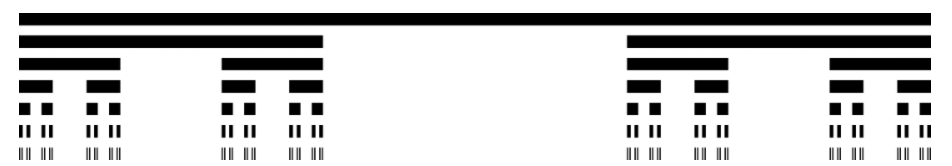
\includegraphics[width=0.65\textwidth]{graphics/Chap05/CantorSet02.png}
}
\hspace{5pt}%
\subfloat[]{%
    \label{fig:CantorSetB}%
	\centering
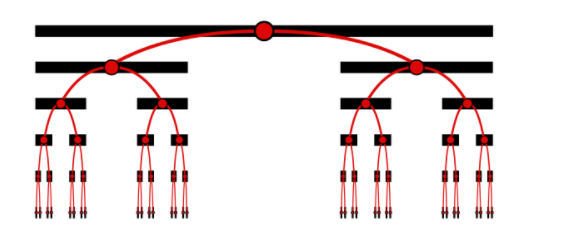
\includegraphics[width=0.3\textwidth]{graphics/Chap05/CantorSet.png}}%
\caption[]{Images of the Cantor set, thanks to Wikipedia. (a) The top line is the interval $[0, 1]$. The line below is what is left when one removes the (open) middle third, $(1/3, 2/3)$. The line below that is what is left when the next two (open) middle thirds, $(1/9, 2/9)$ and $(7/9, 8/9)$, are removed, etc. In the beginning, it's hard to believe that there is anything left over, but there is. In fact, the Cantor set can be placed in one to one correspondence with the original interval $[0,1]$. (b) Shows various paths traced out in a ternary (base 3) expansion of numbers in the Cantor set; ``each point in the Cantor set is uniquely located by a path through an infinitely deep binary tree, where the path turns left or right at each level according to which side of a deleted segment the point lies on. Representing each left turn with 0 and each right turn with 2 yields the ternary  [expansion] for a point'', from Wikipedia \url{https://en.wikipedia.org/wiki/Cantor_set}. Replacing the 2's with 1's  yields a bijection from the Cantor set to the interval $[0, 1]$, which is cool and surprising, though otherwise irrelevant to ROB 501! 
} 
    \label{fig:CantorSet}
\end{figure}

The Cantor set $C \subset [0, 1]$ is a famous set that is uncountable and has Lebesgue measure $0$, 
$$C= \left\{ x \in [0, 1] ~\left|~ x= \sum_{i=1}^\infty  \frac{\epsilon_i}{3^i}, \epsilon_i \in \{0, 2\} \right.  \right\}.$$
The classical construction given in \url{https://en.wikipedia.org/wiki/Cantor_set} shows that it belongs to the Borel sigma algebra. 
% Indeed, if one defines $C_0=[0,1]$, and $ C_{n}:={\frac {C_{n-1}}{3}}\cup \left({\frac {2}{3}}+{\frac {C_{n-1}}{3}}\right)={\frac {1}{3}}{\bigl (}C_{n-1}\cup \left(2+C_{n-1}\right){\bigr )}$, then 
% $$C:=}{\displaystyle {\color {Blue}\lim _{n\to \infty }C_{n}}}{\displaystyle {\color {Blue}\lim _{n\to \infty }C_{n}}}{\displaystyle =\bigcap _{n=0}^{\infty }C_{n}=\bigcap _{n=m}^{\infty }C_{n}}{\displaystyle =\bigcap _{n=0}^{\infty }C_{n}=\bigcap _{n=m}^{\infty }C_{n}}   for any   {\displaystyle m\geq 0}{\displaystyle m\geq 0.
It is impossible to define a uniform probability measure on $[0,1]$ and compute the probability of the Cantor set by performing a Riemann–Stieltjes integral over $C$ because the ``index function'' 
$$ I(x) =  \begin{cases}    1 &  x \in C \\ 0 & \text{ otherwise} \end{cases} $$
has unbounded variation \url{https://en.wikipedia.org/wiki/Bounded_variation}. Said another way, 
$$ P(C) := \underset{ C }{\int}  dx= \int_{0}^{1} I(x)~ dx = \text{ undefined as a Riemann or Riemann–Stieltjes integral}.$$

In any case, whether you are convinced or not, in the rest of this Chapter, we are obliged to be less careful than we have been in other parts of the book. When we discuss the probability of an event and compute it via an integral, we will simply assume that the integral exists within the usual theory of Riemann integration.

\section{First Pass on Probability Basics}
We assume that you may have skipped directly to here.

\subsection{Densities and Random Variables}

\begin{definition}
\label{def:ProbSpaceCopy2}
 $(\Omega, \mathscr{F}, P)$ is called a \textbf{probability space}.
\begin{itemize}
\item $\Omega$ is the sample space. Think of it as the set of all possible outcomes of an experiment. 
\item $E \subset \Omega$ is an event.
\item $\mathscr{F}$ is the collection of allowed events\footnote{Though it is too deep for ROB 501, there are subsets of the reals, for example, that are so complicated one cannot define a reasonable notion of probability that agrees with how we would want to define the probability of an interval, such as $[a, b]$.}. It must at least contain $\emptyset$ and $\Omega$. It is closed with respect to set complement, countable unions, and countable intersections\footnote{By De Morgan's laws, once a set is closed under set complements and countable unions, it is automatically closed under countable intersections; see \url{https://en.wikipedia.org/wiki/De_Morgan}.}. Such sets are called sigma algebras \url{https://en.wikipedia.org/wiki/%CE%A3-algebra}.
    \item $P:\mathscr{F} \to [0, 1]$ is a probability measure. It has to satisfy a few basic operations
    \begin{enumerate}
    \item $P(\emptyset)=0$ and $P(\Omega)=1$.
    \item For each $E\in \mathscr{F}$, $0 \le P(E) \le 1$
    \item If the sets $E_1, E_2, \ldots $ are disjoint (i.e., $E_i \cap E_j = \emptyset$ for $i \neq j$), then
    $$P\big(\bigcup_{i=1}^{\infty}E_i\big) = \sum_{i=1}^{\infty} P(E_i). $$
    \end{enumerate}
    These are typically called the \textbf{Axioms of Probability}.
\end{itemize}
\end{definition}

Shortly, we will define a \emph{probability density}. On the one hand, a density can be viewed as allowing us to define a probability space on the range $\real$ of a random variable $X:\Omega \to \real$. On the other hand, it can be viewed as replacing all of the confusing probability space details with integrals over sets. It is fine to use the latter interpretation.

\begin{figure*}[bth]
	\centering
	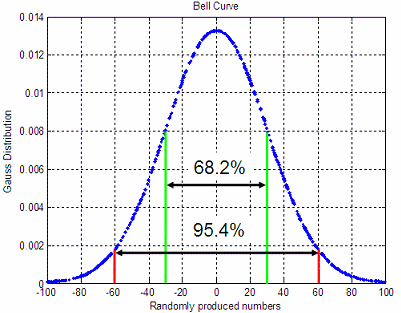
\includegraphics[width=0.35\columnwidth]{graphics/Chap05/gauss-distribution-002.png}~~~~~~ ~~~~
	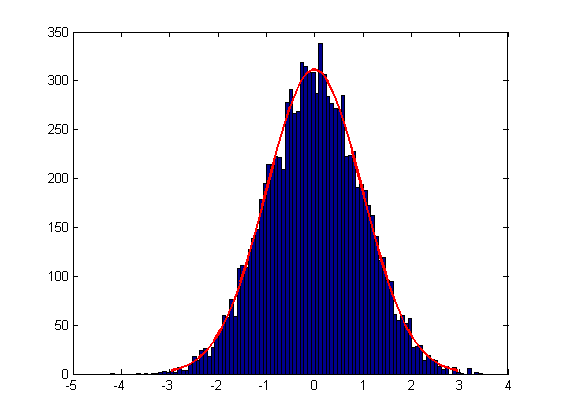
\includegraphics[width=0.35\columnwidth]{graphics/Chap05/O3lCB.png}
	\caption{(Left) Normal distribution $N(\mu, \sigma)$ with $\mu=0$ and $\sigma=30$. (Right) How do you determine the density? You have to collect data! The figure shows a ``fit'' of a normal distribution to data.}
\end{figure*}



\begin{definition} For $E\subset \Omega$, its \textbf{set complement} in $\Omega$ is often denoted in two ways,
$\sim E := E^c := \{ x \in \Omega~~ | ~ x \not \in E\}.$  Similarly, for $A \subset \real$, $\sim A := A^c := \{ x \in \real~ | ~ x \not \in A\}.$
\end{definition}

\begin{definition} A function $X: \Omega \to R$ is a \textbf{random variable} if $\forall ~x \in \real$, the set $\{\omega \in \Omega~| X(\omega) \le x\} \in \mathscr{F} $, that is $P(\{\omega \in \Omega~| X(\omega) \le x\})$ is defined. 
\end{definition}

\emph{With a random variable, we are typically interested in computing the probability that it takes values in a given set $A\subset \real$, that is, we seek to determine $P\{\omega \in \Omega~| X(\omega) \in A\}$.} With the ``frequentist'' interpretation, we are asking how ``frequently'' does $X$ take values in the set $A$. This seems quite difficult to compute because we need to compute first, the inverse image of the set $A$ under the function $X:\Omega \to \real$, 
\begin{equation}
    \label{eq:invImageA}
    \{\omega \in \Omega~| X(\omega) \in A\},
\end{equation}
and then secondly, compute the probability of this set using our probability space $(\Omega, \mathscr{F}, P)$. \emph{The notion of a \emph{density} allows us to circumvent the computation of \eqref{eq:invImageA} and work directly with the set $A$ itself.} \\


% \begin{definition} A (piecewise continuous\footnote{See \url{https://en.wikipedia.org/wiki/Piecewise} A square wave is a piecewise continuous function on $\real$ because one can decompose $\real$ into a countable disjoint union of half-open intervals on which the function is continuous}) function $f:\Omega \to [0, \infty)$ is a \emph{probability density} corresponding to $P$ if $\forall A \in \mathscr{F}$, $P(A) = \underset{ A }{\int} f(x)  dx := \int_{-\infty}^{\infty} I_A(x) f(x) dx$, where $I_A$ is the indicator function. We'll say that $(\Omega, \mathscr{F}, P, f)$ is a probability space with density $f$.
% \end{definition} 

\begin{definition} A (piecewise continuous\footnote{See \url{https://en.wikipedia.org/wiki/Piecewise} A square wave is a piecewise continuous function on $\real$ because one can decompose $\real$ into a countable disjoint union of half-open intervals on which the function is continuous}) function $f:\real \to [0, \infty)$ is a \textbf{probability density} if $\int_{-\infty}^\infty f(x) dx = 1.0$
\end{definition}

\begin{example} Some common densities include
\begin{itemize}
    \item \textbf{Uniform density}: for $a < b$,  $$f(x) = \begin{cases} \frac{1}{b -a} & x \in [a, b] \\ 0 & \text{otherwise}. \end{cases}$$
    \item \textbf{Laplace density}: for $b>0$, $\mu \in \real$, and $x \in (-\infty, \infty)$,
    $$f(x) = \frac{1}{2b} e^{-|x - \mu|/b}.$$
    The parameter $\mu$
 is the mean value, defined below.
 \item \textbf{Gaussian or Normal density}:  for $\sigma>0$, $\mu \in \real$, and $x \in  (-\infty , \infty)$, 
 $$f(x) = \frac{1}{\sigma \sqrt{2 \pi}} e^{-\frac{1}{2} \left( \frac{x - \mu}{\sigma} \right)^2 }.$$ The parameter $\mu$ is the mean value and $\sigma$ is the standard deviation; see below.
 \end{itemize}

\end{example}


\begin{definition} A function $X: \Omega \to R$ is a \textbf{continuous random variable} with density $f:\real \to [0, \infty)$ if 
\begin{enumerate}
\setlength{\itemsep}{.2cm}
\renewcommand{\labelenumi}{(\alph{enumi})}
\item it is a random variable, and 
\item $\forall ~x \in \real$, 
$P(\{\omega \in \Omega~| X(\omega) \le x\})= \int_{-\infty}^x f(\bar{x}) d \bar{x}$.
\end{enumerate}
The lower bound of $-\infty$ is for convenience. It can be replaced with $\inf \{X(\Omega) \subset \real\}$.
\end{definition}

\begin{notation} The notation $X \sim f$ is read as $X$ is distributed with density $f$ or that $X$ is a random variable with density $f$.
\end{notation}


\begin{rem} Useful shorthand notation $\{ X \le x\}:=\{\omega \in \Omega~| X(\omega) \le x\}$ and more generally, for $A\subset \real$, we define $\{ X \in A\}:=\{\omega \in \Omega~| X(\omega) \in A\}$. 
$\hfill \square$  \end{rem} 

\begin{rem} Because $\mathscr{F}$ is closed under set complements, (countable) unions, and (countable) intersections, we can assign probabilities to
\begin{enumerate}
\setlength{\itemsep}{.2cm}
\renewcommand{\labelenumi}{(\alph{enumi})}
     \item $\{ X > x\}=\sim \{ X \le x\} = \{ X \le x\}^{c}$
     \item  $\{ x < X \le y\}= \{ X > x\} \cap  \{ X \le y\}$
\end{enumerate}
and compute them via 
\begin{enumerate}
\setlength{\itemsep}{.2cm}
\renewcommand{\labelenumi}{(\alph{enumi})}
     \item $P(\{ X > x\})= \int_{x}^{\infty} f(x) dx$ and 
     \item  $P(\{ x < X \le y\})=\int_{x}^{y} f(x) dx$, as long as $x \le y$.
\end{enumerate}
These integrals are well defined when $f$ is piecewise continuous.
$\hfill \square$  \end{rem} 


\begin{rem}
For how general of a set $A\subset \real$ can we compute $P(\{ X \in A \})$? To understand this, we note that
\begin{equation}
\label{eq:IntegralOverA}
    P(\{ X \in A \}) :=  \int_{A} f(x) dx := \int_{-\infty}^{\infty} I_A(x) f(x) dx.
\end{equation} 
Because we are limiting ourselves to Riemann-Stiljes integrals, we need $I_A$ to be sufficiently ``nice'' that the product $I_A(x) f(x)$ has bounded variation. A sufficient condition is that $A$
can be expressed as a countable disjoint union of half-open intervals. This seems to be general enough for use in engineering.
$\hfill \square$  \end{rem}


\begin{definition} Moments
 \begin{itemize}
     \item Mean: $\mu:=\E \{ X\}:= \int_{-\infty}^{\infty} x f(x) dx$

     \item Variance: $\sigma^2:=\E \{ (X-\mu)^2)\}:= \int_{-\infty}^{\infty} (x-\mu)^2f(x) dx$ (Var. for short)

     \item Standard Deviation: $\sigma :=\sqrt{\sigma^2}$ (Std. Dev. for short)
     \end{itemize}

\end{definition}
 
% \begin{example}
% \textcolor{red}{\bf Add example for computing stuff.}
% \end{example}

    \subsection{Random Vectors and Densities}
   

\begin{definition}
 Let $(\Omega, \mathscr{F}, P)$ be a probability space. A function $X: \Omega \rightarrow \real^p$ is called a \textbf{random vector} if each component of $X=\left[ \begin{array}{ccc}
        X_1\\X_2\\\vdots\\X_p\end{array} \right]$ is a random variable, that is, $\forall~ 1 \le i \le p$, $X_i: \Omega \rightarrow \real$   is a random variable. 
\end{definition} 

Consequently, $\forall x \in \real^p $, the set $\{\omega \in \Omega \mid X(\omega) \le x\} \in \mathscr{F}$ (i.e., it is an allowed event), where the inequality is understood \textbf{pointwise}, that is,
        $$\{\omega \in \Omega \mid X(\omega) \le x \}:= \left\{\omega \in \Omega ~|~ \begin{bmatrix}X_1(\omega) \\X_2(\omega) \\ \vdots \\ X_p(\omega) \end{bmatrix} \le \begin{bmatrix} x_1 \\x_2 \\ \vdots \\ x_p \end{bmatrix}  \right\} :=\left\{\omega \in \Omega ~~|~~ \begin{bmatrix}X_1(\omega) \le x_1 \\X_2(\omega) \le x_2\\ \vdots \\ X_p(\omega) \le x_p\end{bmatrix} \right\} = \bigcap\limits^p_{i=1} \{\omega \in \Omega \mid X_i(\omega) \le x_i\}.$$

\begin{definition} $X: \Omega \rightarrow \real^p$ is a \textbf{continuous random vector} if there exists a \textbf{density} $f_X:\real^p \to [0, \infty)$ such that,
 $$\forall~x\in \real^P,~~P\big(\{ X \le x\} \big)= \int_{-\infty}^{x_p} ... \int_{-\infty}^{x_2} \int_{-\infty}^{x_1}f_X(\bar{x}_1,\bar{x}_2...\bar{x}_p) d \bar{x}_1 d \bar{x}_2 ... d \bar{x}_p.$$
 More generally, for all $A\subset \real^p$ such that the indicator function $I_A$ has bounded variation,
 $$ P\big(\{ X \in A\} \big)= \int_{-\infty}^{\infty} ... \int_{-\infty}^{\infty} \int_{-\infty}^{\infty} I_A(\bar{x}_1,\bar{x}_2...\bar{x}_p) f_X(\bar{x}_1,\bar{x}_2...\bar{x}_p) d \bar{x}_1 d \bar{x}_2 ... d \bar{x}_p.$$
\end{definition} 

\begin{notation} The notation $X \sim f$ is read as $X$ is distributed with density $f$ or that $X$ is a random vector with density $f$.
\end{notation}



\begin{definition} (Moments) Suppose $g: \real^p \to \real^k$
        $$\E\{g(X)\}:=\int_{\real^p}g(x)f_X(x)dx:=\int_{-\infty}^{\infty}...\int_{-\infty}^{\infty}g(x_1,...,x_p)f_X(x_1,...,x_p)dx_1...dx_p$$
\begin{itemize}
    \item  \textbf{Mean or Expected Value}$$\mu=\E\{X\}=\E\{\left[ \begin{array}{ccc}X_1\\\vdots\\X_p\end{array} \right]\}=\left[ \begin{array}{ccc}\E\{X_1\}\\\vdots\\ \E\{X_p\}\end{array} \right]=
        \left[ \begin{array}{ccc}\mu_1\\\vdots\\\mu_p \end{array} \right]$$
\item 
        \textbf{Covariance Matrices}$$\Sigma:={\rm cov}(X)={\rm cov}(X,X)=\E\{(X-\mu)(X-\mu)^T\}$$
        where $(X-\mu) \mbox{ is }p\times 1 \mbox{, } (X-\mu)^T \mbox{ is }1\times p\mbox{, } (X-\mu)(X-\mu)^T \mbox{ is }p\times p$
        
        \item \textbf{Variance:} ${\rm Var}(X):= \tr \Sigma := \sum_{i=1}^{p} \Sigma_{ii}$, where $\Sigma$ is the covariance of $X$.

\end{itemize}

\end{definition}
       
\begin{exercise}
  $\Sigma:={\rm cov}(X)={\rm cov}(X,X)$ is a positive semi-definite matrix.
\end{exercise}

\textbf{Solution:} For $ v \in \real^p$, we need to show that $v^\top \Sigma v\ge 0$, where $\Sigma := \E \{(X-\mu) \cdot (X-\mu)^\top \}$. 
\begin{align*}
    v^\top \Sigma v:=& v^\top \E \{(X-\mu) \cdot (X-\mu)^\top \} v \\ 
    =&  \E \{v^\top(X-\mu) \cdot (X-\mu)^\top v\}  \\
    =& \E \{ \left((X-\mu)^\top v\right)^\top \cdot \left((X-\mu)^\top v \right)\} \\
    =& \E\{|| (X-\mu)^\top v ||^2  \} \\
    =& \int_{\real^p} || (X-\mu)^\top v ||^2 f_X(x) dx \\
    \ge& ~ 0
\end{align*}
because the integral of a non-negative function over $\real^p$ is non-negative.
\Qed

\begin{definition} If $\Sigma >0$, then $\Sigma^{-1}$ is called the \textbf{information matrix}. The interpretation is that ``high variance'' means ``low information'' and vice versa.
\end{definition}

  
        
\section{Estimators}

\subsection{Best Linear Unbiased Estimator (BLUE)}

\textbf{Model:} The measurement is $y=Cx+\varepsilon$, $y\in \mathbb{R}^m$, $x \in \mathbb{R}^n$, $\E\{\varepsilon\}=0$, $\cov\{\varepsilon,\varepsilon\}=\E\{\varepsilon \varepsilon^\top \}=Q>0$, and
the columns of $C$ are linearly independent. \emph{We assume no stochastic (random) model for the unknown $x$.} In other words, $x\in \real^n$ is an unknown deterministic vector. It is emphasized that $\varepsilon$ and hence $y$ are random vectors while $x$ is not a random vector. Do not let the lowercase symbols being used for $y$, $\epsilon$, and $x$ distract you.\\

    \textbf{Seek:} An estimate $\widehat{x}$ of $x$ that satisfies:
    \begin{enumerate}
        \item \ul{Linear:} $\widehat{x}=Ky$ for some $n \times m$ matrix $K$.
        \item \ul{Unbiased for all $x\in \real^n$:} $\E\{ \widehat{x} - x \} =0 $ holds for all $x\in \real^n$. It needs to hold for all $x$ because $x$ can be an arbitrary value in $\real^n$.
        \item \ul{Best:} $\widehat{x}$ minimizes  $\E\{(\widehat{x} - x)^\top (\widehat{x} -x)\}=\E\{ \sum \limits_{i=1}^n |\widehat{x_i}-x_i|^2\} $, the variance of $\widehat{x} - x$.
    \end{enumerate}
    
\begin{claim} A linear estimate $\widehat{x}=Ky$ is unbiased if, and only if $KC=I$.
\end{claim}
\textbf{Proof:} 
\begin{align*}
    0 & = \E\{ \widehat{x} - x\} ~\forall x \in \real^n\\
    & \Updownarrow \\
     0 & = \E\{ Ky - x\}  ~\forall x \in \real^n\\
    & \Updownarrow \\
     0 & = \E\{ K(Cx+\varepsilon) - x\}  ~\forall x \in \real^n\\
    & \Updownarrow \\
        0 & = \E\{ (K C - I)x\} - \E\{K \varepsilon \}  ~\forall x \in \real^n \\
    & \Updownarrow \\
            0 & = (K C - I)x  ~\forall x \in \real^n\\
\end{align*}
where we used $\E\{\varepsilon\}=0$ by assumption and $ \E\{ (K C - I)x\}=(K C - I)x$ because $x$ is deterministic. Finally, $0=(K C - I)x  ~\forall x \in \real^n \iff KC-I =0_{n \times n}$ as can be seen by taking $x = e^i$, for $1 \le i \le n$.

$\hfill \square$


    \textbf{Aside:}~ For $v, w \in \real^n$, $ (v+w)^\top (v+w)=v^\top v+w^\top w+v^\top w+w^\top v =
        v^\top v+w^\top w+2v^\top w$ because $v^\top w $ is a scalar.\\
        
        Therefore, for an unbiased linear estimator,

    \begin{align*}
\E\{(\widehat{x} - x)^\top (\widehat{x} -x)\}& =\E\{(KCx-x+K\varepsilon)^\top (KCx-x+K\varepsilon)\}\\
        & =\E\{x^\top(KC - I)^\top(KC-I)x+2(K\varepsilon)^\top(KC-I)x+\varepsilon^\top  K^\top  K \varepsilon\} \\
         & =\E\{2(K\varepsilon)^\top(KC-I)x+\varepsilon^\top  K^\top  K \varepsilon\}\\
         &= \E\{ \varepsilon^\top  K^\top  K \varepsilon\}
    \end{align*}
Moreover, by using the properties of the trace, we have
    \begin{equation*}
        \varepsilon^\top K^\top K\varepsilon= \tr\left( \varepsilon^\top K^\top K\varepsilon \right)=\tr\left(K\varepsilon\varepsilon^\top K^\top\right).
    \end{equation*}
    and therefore,
    \begin{align*}
\E\{(\widehat{x} - x)^\top (\widehat{x} -x)\}&=\tr\E\{K\varepsilon\varepsilon^\top K^\top\}\\
        &=\tr(KQK^\top ).
    \end{align*}
Hence, 
$$ 
  \widehat{K}=\argmin_{KC = I}  \E\{(\widehat{x} - x)^\top (\widehat{x} -x)\} \iff     \widehat{K}=\argmin_{KC = I}  \tr(KQK^\top) 
$$

    \textbf{A simplifying observation:} If we partition $K$ into rows via 
    $$K= \begin{bmatrix}
        k_1\\
        k_2\\
        \vdots\\
        k_n
    \end{bmatrix}$$
then $K^\top =\begin{bmatrix}
        k_1^\top &   \dotsb &  k_n^\top
    \end{bmatrix}$
    and $ \tr\left(\begin{bmatrix}
            {k_1}\\
            \vdots\\
            {k_n}
            \end{bmatrix}Q\begin{bmatrix}k_1^\top & \dotsb& k_n^\top\end{bmatrix}\right) =\sum^{n}_{i=1}k_iQk_i^\top$. Moreover, 
    \begin{align*}
        KC= I_{n\times n} &\iff C^\top K^\top =I_{n\times n}\\
        &\iff C^\top \begin{bmatrix}k_1^\top &  \dotsb & k_n^\top\end{bmatrix}=\begin{bmatrix}e_1 & \dotsb & e_n\end{bmatrix}\\
        &\iff C^\top k_i^\top=e_i\ \ \ \ 1\leq i\leq n.
    \end{align*}
Hence, we have $n$-separate optimization problems involving the column vectors $k_i^\top $, namely
    \begin{equation*}
        \widehat{k}_i^\top = \argmin_{C^\top k_i^\top=e_i} k_i Q k_i^\top, ~1 \le i \le n.
    \end{equation*}
    From Proposition~\ref{prop:UnderDetermined} for underdetermined equations, we have
$$\widehat{k}_i^\top = Q^{-1}C(C^\top Q^{-1}C)^{-1}e_i,$$
which yields
$$ \widehat{K}^\top = \begin{bmatrix} \widehat{k}_1^\top & \cdots & \widehat{k}_n^\top \end{bmatrix}=Q^{-1}C(C^\top Q^{-1}C)^{-1}.$$
    \newline
    Therefore,
    \begin{equation*}
      \widehat{K}= (C^\top Q^{-1}C)^{-1}C^\top Q^{-1}.
      \end{equation*}
\vspace*{.2cm}

\begin{thm} \textbf{(BLUE)}
     Let $x\in\real^n$, $y\in\real^m$, $y=Cx+\varepsilon$, $\E\{\varepsilon\}=0$, $\E\{\varepsilon\varepsilon^\top\}=:Q>0$, and $\rank(C)=n$. The Best Linear Unbiased Estimator (BLUE) is $\widehat{x}=\widehat{K}y$ where
    \begin{equation*}
        \widehat{K}=\left(C^\top Q^{-1}C\right)^{-1}C^\top Q^{-1}.
    \end{equation*}
    Moreover, the covariance of the error is
    \begin{equation*}
        \E\{\left(\widehat{x}-x\right)\left(\widehat{x}-x\right)^\top\}=\left(C^\top Q^{-1}C\right)^{-1}.
    \end{equation*}

\end{thm}

\textbf{Proof:} The only thing left to show is the error covariance. From previous calculations,
    \begin{align*}
        \widehat{x}-x&=Ky-x\\
        &=KCx+K\varepsilon-x\\
        &=K\varepsilon~(\text{because}~KC=I)\\
        \therefore \E\{(\widehat{x}-x)(\widehat{x}-x)^\top\}&=\E\{(K\varepsilon)(K\varepsilon)^\top\}\\
        &=\E\{K\varepsilon\varepsilon^\top K^\top\}\\
        &=KQK^\top
    \end{align*}
    Hence, 
    \begin{align*}
        \E\{\left(\widehat{x}-x\right)\left(\widehat{x}-x\right)^\top\}&=KQK^\top\\
        &=\left(C^\top Q^{-1}C\right)^{-1}C^\top Q^{-1}QQ^{-1}C\left(C^\top Q^{-1}C\right)^{-1}\\
        &=\left(C^\top Q^{-1}C\right)^{-1}\left[C^\top Q^{-1}C\right]\left(C^\top Q^{-1}C\right)^{-1}\\
        &=\left(C^\top Q^{-1}C\right)^{-1}.
    \end{align*}
    
    \Qed
    
\begin{rem} \emph{Comparing Weighted Least Squares to BLUE:}
\begin{itemize}
    \item They are \ul{identical} when the weighting matrix is taken as the \ul{inverse} of the covariance matrix of the noise term: $W=Q^{-1}$. The inverse of the covariance matrix is called the \textit{information} matrix. Hence, there is low information when the variance (or covariance) is large.

        \item Another way to say this, if you solve a least squares problem with weight matrix $W>0$, you are implicitly assuming that your uncertainty in the measurements has zero mean and a covariance matrix of $Q=W^{-1}$.

            \item If you know the uncertainty has zero mean and a covariance matrix of $Q$, using $W=Q^{-1}$ makes a lot of sense. For simplicity, assume that $Q$ is diagonal. A large entry in $Q$ means high variance, which means the measurement is highly uncertain. Hence, the corresponding component of $y$ should not be weighted very much in the optimization problem....and indeed, taking $W=Q^{-1}$ does just that because, the weight term $W$ is small for large terms in $Q$.
            
            \item Weighted least squares was based on overdetermined systems of linear equations. To derive BLUE, we needed to understand  underdetermined systems of linear equations. That's kind of cool!
    \end{itemize}
       
$\hfill \square$  \end{rem}
    
 \subsection{Minimum Variance Estimator (MVE)}   
 
 \textbf{Model:} $y=Cx+\varepsilon, y\in \mathbb{R}^m, x \in \mathbb{R}^n, \text{and}~ \varepsilon\in \mathbb{R}^m,$ with the following stochastic assumptions:
 \begin{itemize}
     \item Zero Means: $E\{x\}=0, E\{\varepsilon\}= 0$. 
     \item Covariances: $E\{\varepsilon \varepsilon^\top \}=Q, E\{xx^\top \}= P, E\{\varepsilon x^\top \}=0$.
 \end{itemize}

\begin{rem}
       $E\{\varepsilon x^\top \}=0$ means that the state variables and noise terms are uncorrelated. Recall that uncorrelated does NOT imply independence, except for Gaussian random vectors.
$\hfill \square$  \end{rem} 

\textbf{Assumption:}  $Q\ge 0$, $P \ge 0$, and $CPC^\top +Q >0$.  (Will see why later.) We note that $Q>0 \implies CPC^\top +Q >0$ for all $m \times n$ matrices $C$. If $Q>0$, we do not need to assume the columns of $C$ are linearly independent. In fact, $C = 0_{m \times n}$ is possible.\\

\textbf{Objective:} We seek $\widehat{x}$ that minimizes the variance
$$E\{(\widehat x -x)^\top (\widehat x -x)\} = E\{ \sum\limits_{i=1}^n (\widehat x_i-x_i)^2\} = \sum\limits_{i=1}^n E\{ (\widehat x_i-x_i)^2 \}.$$

\begin{rem} As for BLUE, we see that there are $n$ separate optimization problems.
       We also see that a linear estimate $\widehat x = Ky$ would be automatically unbiased, because
$$ E\{\widehat x - x\}=E\{ Ky - x\} = E\{ KCx+K\varepsilon - x\} = (KC-I) E\{x\}+KE\{\varepsilon\}  = 0,$$
without imposing that $KC = I$. 
$\hfill \square$  \end{rem}


\textbf{Problem Formulation (the Unexpected Inner Product):} We will pose this as a minimum norm problem in an inner product space of random variables. Suppose that 
$$x=   \begin{bmatrix}
    x_1\\
    \vdots\\
    x_n
  \end{bmatrix}~~~\text{and} ~~~~\varepsilon =   \begin{bmatrix}
    \varepsilon_1\\
    \vdots\\
    \varepsilon_m
  \end{bmatrix}.$$
  We recall that components of random vectors are random variables. Hence, $x_i$, $1 \le i \le n$ and $\varepsilon_j$, $1 \le j \le m$ are all random variables, and hence are \textbf{functions}.
  We define ${\cal F} = \mathbb{R},$ and $\mathcal{X} = span\{x_1, x_2, \dots , x_n, \varepsilon_1, \varepsilon_2, \dots, \varepsilon_m\},$ and for  $z_1,z_2 \in \mathcal{X}$, we \underline{define their inner product} by  $$<z_1,z_2> := E\{z_1z_2\}.$$
  We note that $\forall~ z \in \mathcal{X}$, $\E\{z\}=0$ and $\var(z)=<z,z>$. \textbf{Hence, this inner product space is designed to treat minimum variance optimization problems.}
  
  \begin{rem}
  $$ E\{z_1z_2\} = \begin{cases} P_{ij} & z_1 = x_i, z_2 = x_j \\  Q_{ij} & z_1 = \varepsilon_i, z_2=\varepsilon_j \\ 0 &  z_1 = x_i, z_2=\varepsilon_j \\ 0 &  z_1 = \varepsilon_i, z_2=x_j. \end{cases}$$
  $\hfill \square$  \end{rem}

\textbf{Define:} \\
$M = \spanof{y_1,y_2,\dots,y_m} \subset \mathcal{X}$ ($M$ is the subspace spanned by the measurements),\\

$y_i = C_ix+\varepsilon_i = \sum\limits_{j=1}^n C_{ij}x_j+\varepsilon_i, 1\le i \le m,$  ($i$-th row of $y$)\\

$\widehat{x}_i = \argmin\limits_{m \in M} \|x_i-m\|^2 =  \argmin \limits_{m \in M}  \langle x_i-m, x_i-m \rangle $\\


\textbf{Fact:} $\{y_1,y_2,\dots,y_m\}$ is linearly independent if, and only if, $CPC^\top +Q$ is positive definite. This is proven below when we compute the Gram matrix. (Recall, $\{y_1,y_2,\dots,y_m\}$ linearly independent if, and only if $G$ is full rank, where $G_{ij}:=<y_i,y_j>.$)\\


\textbf{ Solution via the Normal Equations:} By the normal equations,
$$\widehat{x}_i = \widehat \alpha_1 y_1  +  \widehat \alpha_2 y_2  + \dots + \widehat \alpha_m y_m$$
where $G^\top \widehat \alpha = \beta$ and
\begin{align*}
G_{ij} = <y_i,y_j> = E\{y_i y_j\} &= E\{[C_i x+\varepsilon_i][C_j x+\varepsilon_j]\}\\
& = E\{[C_i x+\varepsilon_i][C_j x+\varepsilon_j]^\top \}\\
& = E\{[C_i x+\varepsilon_i][x^\top  {C_j}^\top  +\varepsilon_j]\}\\
& = E\{C_i xx^\top  C_j^\top \} + E\{C_i x\varepsilon_j\} + E\{\varepsilon_i x^\top  C_j^\top \} + E\{ \varepsilon_i \varepsilon_j\}\\
& = C_iE\{ xx^\top  \}C_j^\top  + E\{ \varepsilon_i \varepsilon_j\}\\
& = C_i P C_j^\top  + Q_{ij}\\
&=[CPC^\top +Q]_{ij}\
\end{align*}
where we have used the fact that $x$ and $\varepsilon$ are uncorrelated. We conclude that
$$G = CPC^\top +Q.$$

We now turn to computing $\beta$. Let's note that $x_i$, the $i$-th component of $x$, is equal to $x^\top  e_i$, where $e_i$ is the standard basis vector in $\real^n$.
\begin{align*}
\beta_j = <x_i,y_j> &= E\{x_i y_j\}\\
 &= E\{x_i[C_j x+\varepsilon_j]\} \\
 &= E\{x_i C_j x\} + E\{x_i \varepsilon_j\} \\
 & = C_jE\{ x x_i\} \\
  & = C_jE\{ x x^\top  e_i\} \\
    & = C_jE\{ x x^\top  \} e_i\\
 &= C_j P e_i \\
 &= C_j P_i
\end{align*}
where $P=\begin{bmatrix} P_1 & P_2 &  \cdots & P_n \end{bmatrix}$, and hence $P_i$ is the $i$-th column of $P$. Putting all of this together, we have
\begin{align*}
G^\top \widehat \alpha &= \beta \\
&\Updownarrow \\
[CPC^\top +Q] \widehat \alpha &= C P_i \\
&\Updownarrow \\
\widehat \alpha &= [CPC^\top +Q]^{-1} C P_i
\end{align*}


$\widehat{x}_i = \widehat \alpha_1 y_1  +  \widehat \alpha_2 y_2  + \dots + \widehat \alpha_m y_m = \widehat \alpha^\top  y=$ (row vector $\times$ column vector), where
$$\widehat \alpha =   \begin{bmatrix}
    \widehat \alpha_1\\
    \vdots\\
    \widehat \alpha_m
  \end{bmatrix}.$$

We now seek to identify a gain matrix $K$ so that
$$\widehat x = Ky \iff \widehat x_i = K_i y, \text{where}~~K =    \begin{bmatrix}
   {K_1}\\
{K_2}\\
    \vdots\\
  {K_n}
  \end{bmatrix};$$
  that is, $K_i$ is the $i$-th row of $K$.

  \begin{align*}
    K_i^\top  = \widehat \alpha_i &=  [CPC^\top +Q]^{-1} C P_i, 1 \le i \le n\\
    &\Updownarrow\\
   \begin{bmatrix} K_1^\top  & \cdots & K_n^\top  \end{bmatrix} &= [CPC^\top +Q]^{-1} C P\\
   &\Updownarrow\\
   K^\top &=  [CPC^\top +Q]^{-1} C P\\
   &\Updownarrow\\
    K&=PC^\top [CPC^\top +Q]^{-1}\
\end{align*}

$$\boxed{\widehat{x} = K y =  PC^\top [CPC^\top +Q]^{-1}y}$$

\begin{thm} \textbf{(Minimum Variance Estimator)}
\label{thm:MVE}
     Let $x\in\real^n$, $y\in\real^m$, $y=Cx+\varepsilon$,  with the following stochastic assumptions:
 \begin{itemize}
     \item Zero Means: $E\{x\}=0, E\{\varepsilon\}= 0$. 
     \item Covariances: $E\{\varepsilon \varepsilon^\top \}=Q, E\{xx^\top \}= P, E\{\varepsilon x^\top \}=0$.
 \end{itemize} 
The Minimum Variance Estimator (MVE) is $\widehat{x}=\widehat{K}y$ where
    \begin{equation*}
        \widehat{K}=PC^\top [CPC^\top +Q]^{-1}.
    \end{equation*}
    Moreover, the covariance of the error is
    \begin{equation*}
        \E\{\left(\widehat{x}-x\right)\left(\widehat{x}-x\right)^\top\}=P-PC^\top [CPC^\top +Q]^{-1}CP.
    \end{equation*}

\end{thm}

\textbf{Proof:} The only thing left to show is the error covariance. From previous calculations,  let's note that
$$\widehat x -x = Ky-x = KC x + K \varepsilon  - x=(KC - I)x + K \varepsilon $$
and thus
$$ (\widehat x -x)(\widehat x -x)^\top= (KC - I)x x^\top (KC - I)^\top + K \varepsilon \varepsilon^\top K^\top - (KC - I)x \varepsilon^\top K^\top - K\varepsilon x^\top (KC - I)^\top.  $$

Taking expectations, and recalling that $x$ and $\varepsilon$ are uncorrelated, we have
\begin{align*}
E\{(\widehat x -x)(\widehat x -x)^\top \} & = (KC-I) P (KC-I)^\top + K Q K^\top \\
&= KC P C^\top K^\top + P - 2 PC^\top K^\top + K Q K^\top\\
&= P + K [CPC^\top + Q] K^\top  -2 PC^\top K^\top.
\end{align*}
Substituting with $K=PC^\top [CPC^\top +Q]^{-1}$ and simplifying yields the result.
\Qed

\newpage

\begin{rem} \mbox{ }

\begin{enumerate}
\item $\cov(\begin{bmatrix} x \\ y \end{bmatrix}) = \E\{\ \left[\begin{array}{c} x \\ Cx + \varepsilon  \end{array} \right] \left[\begin{array}{cc} x^\top & x^\top C^\top + \varepsilon^\top \end{array} \right] \} = \left[\begin{array}{cc} P & P C^\top \\ C P & CPC^\top + Q \end{array} \right].$

\item Hence, we see that the covariance of the error $\widehat{x}-x$ is the Schur Complement of $\cov(x)$  in  $\cov(\begin{bmatrix} x \\ y \end{bmatrix})$. 

\item The term $PC^\top [CPC^\top +Q]^{-1}CP$ represents the ``value'' of the measurements. It is the reduction in the covariance of $x$ given the measurement $y$.

\item If $Q>0$ and $P>0$, then from the Matrix Inversion Lemma
$$\boxed{\widehat x = Ky = [C^\top Q^{-1}C+P^{-1}]^{-1}C^\top Q^{-1}y.}$$
This form of the equation is useful for comparing BLUE vs MVE

\item \textbf{BLUE vs MVE:}\\

\begin{itemize}

\item \textbf{BLUE:} $\widehat x = [C^\top  Q^{-1}C]^{-1}C^\top  Q^{-1}y$ \\

\item \textbf{MVE:} $\widehat x = [C^\top  Q^{-1}C+P^{-1}]^{-1}C^\top  Q^{-1}y$ \\

\item Hence, BLUE = MVE when $P^{-1} = 0$.\\

\item $P^{-1} = 0$ roughly means $P= \infty I$, that is infinite covariance in $x$, which in turn means we have \textit{no idea} about how $x$ is distributed.\\

    \item For BLUE to exist, we need $\dim(y) \ge \dim(x) $\\

    \item For MVE to exist, we can have $\dim(y) < \dim(x) $ as long as $(C P C^\top + Q) >0$.

\end{itemize}

\end{enumerate}

       
$\hfill \square$  \end{rem}

\begin{rem} (Solution to MIL) We will show that if $Q>0$ and $P>0$, then 
$$ PC^\top [CPC^\top +Q]^{-1}= [C^\top  Q^{-1}C+P^{-1}]^{-1}C^\top  Q^{-1}.$$

Recall the MIL: Suppose that $A$, $B$, $C$ and $D$ are compatible\footnote{The sizes are such the matrix products and sum in $A+BCD$ make sense.} matrices. If $A$, $C$, and  $(C^{-1}+D A^{-1}B)$ are each square and invertible, then  $A+BCD$ is invertible and
    $$ (A + BCD)^{-1} = A^{-1} - A^{-1}B(C^{-1} + DA^{-1}B)^{-1}DA^{-1}.$$

We apply the MIL to $[C^\top  Q^{-1}C+P^{-1}]^{-1}$, where we identify $A=P^{-1}, B=C^\top, C=Q^{-1}, D=C$. This yields
$$[C^\top  Q^{-1}C+P^{-1}]^{-1} = P-PC^\top [ Q + CPC^\top]^{-1} CP.$$
Hence,
\begin{align*}
[C^\top  Q^{-1}C+P^{-1}]^{-1}C^\top  Q^{-1} &= PC^\top  Q^{-1}-PC^\top [ Q + CPC^\top]^{-1} CPC^\top  Q^{-1} \\
&= PC^\top \left[ I - [Q+CPC^\top]^{-1} CPC^\top   \right] Q^{-1} \\
&={\scriptstyle  PC^\top \left[ [Q+CPC^\top]^{-1} [Q+CPC^\top] - [Q+CPC^\top]^{-1} CPC^\top   \right] Q^{-1}}\\
&=PC^\top [Q+CPC^\top]^{-1} \left[  [Q+CPC^\top] - CPC^\top   \right] Q^{-1}\\
&= PC^\top [Q+CPC^\top]^{-1} \left[  Q+CPC^\top - CPC^\top   \right] Q^{-1}\\
&= PC^\top [Q+CPC^\top]^{-1} \left[  Q    \right] Q^{-1}\\
&= PC^\top [Q+CPC^\top]^{-1}
\end{align*}

$\hfill \square$  
\end{rem}

\section{Second Pass on Probability Basics}
    
    
   \subsection{Marginal Densities, Independence, and Correlation}
        Suppose the random vector $X: \Omega \rightarrow \real^p$ is partitioned into two components $X_1 : \Omega \rightarrow R^n$ and $X_2:\Omega \rightarrow R^m $, with $p=n+m$, so that,
        $$ X = \left[ \begin{array}{cc} X_1 \\
                                               X_2 \end{array} \right]$$

\begin{notation} We denote the density of $X$ by

$$f_X(x)=f_{\small \left[ \begin{array}{cc} X_1 \\
                                               X_2 \end{array} \right]}(x_1,x_2)=f_{X_1 X_2}(x_1,x_2) $$

and it is called the \textbf{joint density} of $X_1$ and $X_2$. As before, we can define the mean and covariance.
\begin{itemize}

 \item Mean is $\mu=
        \left[ \begin{array}{ccc}\mu_1\\ \mu_2 \end{array} \right]= \E\{X\}=\E\{\left[ \begin{array}{ccc}X_1\\ X_2\end{array} \right]\}=\left[ \begin{array}{ccc}\E \{X_1\}\\ \E\{X_2\}\end{array} \right]$

 \item Covariance is \begin{align*} \Sigma =    \left[ \begin{array}{cc}\Sigma_{11} & \Sigma_{12}\\ \Sigma_{21} & \Sigma_{22}\end{array} \right] &= \E\{\left[ \begin{array}{c}X_1-\mu_1\\ X_2-\mu_2\end{array} \right] \left[ \begin{array}{c}X_1-\mu_1\\ X_2-\mu_2\end{array} \right]^\top\}  \\
     &= \E\{\left[ \begin{array}{c}X_1-\mu_1\\ X_2-\mu_2\end{array} \right] \left[ (X_1-\mu_1)^\top~~~ (X_2-\mu_2)^\top  \right] \} \\
     &= \E\{\left[ \begin{array}{cc}(X_1-\mu_1)(X_1-\mu_1)^\top &(X_1-\mu_1)(X_2-\mu_2)^\top \\
     (X_1-\mu_1)(X_2-\mu_2)^\top &(X_2-\mu_1)(X_2-\mu_2)^\top
     \end{array} \right]
     \end{align*}
 \end{itemize}
 where $\Sigma_{12}=\Sigma_{21}^\top = cov(X_1,X_2)=\E\{ (X_1-\mu_1)(X_2-\mu_2)^\top  \}$ is also called the \textbf{correlation} of $X_1$ and $X_2$.

\end{notation}

 If $X = \left[ \begin{array}{cc} X_1 \\
                                               X_2 \end{array} \right] :\Omega \to \real^{n+m}$ is a continuous random vector, then its components
                                               $$X_1:\Omega \to \real^n~~\text{and}~~X_2: \Omega \to \real^m$$ are also continuous random vectors and have densities, $f_{X_1}(x_1)$ and $f_{X_2}(x_2)$. These densities are given a special name. 

\begin{definition} $f_{X_1}(x_1)$ and $f_{X_2}(x_2)$  are called the \textbf{marginal densities} of $X_1$ and $X_2$.
       
\end{definition}

\begin{fact} In general the marginal densities are a nightmare to compute.  \begin{align*} f_{X_1}(x_1) &:= \int_{-\infty}^{\infty} f_{X_1 X_2}(x_1, x_2) d x_2  \medskip \\
 &: =\int_{-\infty}^{\infty} \cdots \int_{-\infty}^{\infty} f_{X_1X_2}\big( \underbrace{ \bar{x}_1, \ldots, \bar{x}_n }_{x_1}, \underbrace{ \bar{x}_{n+1} , \cdots, \bar{x}_{n+m}}_{x_2} \big) \underbrace{d\bar{x}_{n+1} \cdots d\bar{x}_{n+m}}_{dx_2}\\
 \\
 f_{X_2}(x_2) &:= \int_{-\infty}^{\infty} f_{X_1 X_2}(x_1, x_2) d x_1  \medskip \\
 &: =\int_{-\infty}^{\infty} \cdots \int_{-\infty}^{\infty} f_{X_1X_2}\big( \underbrace{ \bar{x}_1, \ldots, \bar{x}_n }_{x_1}, \underbrace{ \bar{x}_{n+1} , \cdots, \bar{x}_{n+m}}_{x_2} \big) \underbrace{d\bar{x}_{1} \cdots d\bar{x}_{n}}_{dx_1}\\
\end{align*}
For Normal Random Vectors, however, we can read the marginal densities directly from the joint density! We will not be doing any iterated integrals in ROB 501.
 
$\hfill \square$  \end{fact} 

\begin{definition} Random vectors $X_1$ and $X_2$ are \textbf{independent} if their joint density factors
        $$f_X(x)=f_{X_1 X_2}(x_1,x_2)=f_{X_1}(x_1)f_{X_2}(x_2).$$

$X_1$ and $X_2$ are \textbf{uncorrelated} if their ``cross covariance'' or ``correlation '' is zero, that is, 
        $$cov(X_1,X_2) := \E \{ (X_1-\mu_1)(X_2-\mu_2)^\top \} = 0_{n \times m}.$$
       
\end{definition}

\begin{fact} If random vectors $X_1$ and $X_2$ are independent, then they are also uncorrelated. \textcolor{red}{\bf The converse is in general false.}
$\hfill \square$
\end{fact} 

\subsection{Conditional Probabilities}

\begin{definition} Consider two events $A,B \in \mathscr{F}$, with $P(B) > 0$. The \textbf{conditional probability of $A$ given $B$} is
        $$P(A \mid B):=\frac{P(A\bigcap B)}{P(B)}.$$
\end{definition} 

\begin{rem} Suppose $A$ is the event that our robot is near a certain location and $B$ is the event that our robot has been cited by a particular camera. These two events have individual probabilities $P(A)$ and $P(B)$. The \textbf{conditional probability of event $A$ given that event $B$ occurred is how we ``fuse'' the two pieces of information},
        $$P(A \mid B):=\frac{P(A\bigcap B)}{P(B)}.$$
As an example, suppose we define a uniform probability across all floors of FRB, which has a total surface area of roughly 12,000 $m^2$ (roughly, 120,000 square feet) and let $A$ be the event our robot is choosing a snack in the self-service section of the Eigen Cafe. Well, the area of the self-service section of the Eigen Cafe is roughly 8 $m^2$, and thus $P(A) \approx 6.66~10^{-4}$. We'll now let $B$ be the event that our robot has been seen (i.e, measured to be) at the Eigen Cafe. The total area of the Eigen Cafe is approximately 30 $m^2$. Hence, $P(B)\approx 2.5~ 10^{-3}$. Because $A \subset B$, it follows that $A \cap B = A$ and hence
    $$P(A \mid B)=\frac{P(A\bigcap B)}{P(B)} = \frac{P(A)}{P(B)}= \frac{6.66~10^{-4}}{2.5~ 10^{-3}}=0.266.$$
    We note that $P(A \mid B)=0.266$ is a lot more certain than $P(A) \approx 6.66~10^{-4}$. Hence, as you can now imagine, conditional probabilities are very important in engineering.
$\hfill \square$  \end{rem}

\begin{rem} Special cases:
\begin{itemize}
        \item
        $B\subset A \mbox{, } P(A \mid B)=\frac{P(A\bigcap B)}{P(B)}=\frac{P(B)}{P(B)}=1$
        \item
        $A\subset B \mbox{, } P(A \mid B)=\frac{P(A\bigcap B)}{P(B)}=\frac{P(A)}{P(B)}\ge P(A)$

        \end{itemize}
        
$\hfill \square$  \end{rem}
   
   \begin{definition} Consider again our partitioned random vector 
   $ X = \left[ \begin{array}{cc} X_1 \\ X_2 \end{array} \right]$. The \textbf{conditional density of $X_1$ given $X_2 = x_2$} is
          $$f_{X_1\mid X_2}(x_1 \mid x_2):=\frac{f_{X_1X_2}(x_1,x_2)}{f_{X_2}(x_2)}.$$
        Sometimes, for brevity, we simply write $f(x_1 \mid x_2)$.
 \end{definition} 
 
 \begin{rem} \textbf{Remarks on Conditional Random Vectors:}
        \begin{itemize}

        \item \textbf{Very important:} $X_1$ given $X_2=x_2$ is (still) a random vector. It's density is $f_{X_1\mid X_2}(x_1 \mid x_2)$

        \item \textbf{Conditional Mean:} \begin{align*} \mu_{X_1 \mid X_2=x_2}&:=\E \{ X_1 \mid X_2=x_2\}  \\ &:=\int_{-\infty}^{\infty} x_1 f_{X_1\mid X_2}(x_1 \mid x_2) dx_1
            \end{align*}
            $\mu_{X_1 \mid X_2=x_2}$ is a function of $x_2$. Think of it as a function of the value read by your sensor.

         \item  \textbf{Conditional Covariance:} \begin{align*} \Sigma_{X_1 \mid X_2=x_2} & := \E \{ (X_1 -\mu_{X_1 \mid X_2=x_2})(X_1 -\mu_{X_1 \mid X_2=x_2})^\top \mid X_2=x_2 \} \\ \\ &:=\int_{-\infty}^{\infty} (X_1 -\mu_{X_1 \mid X_2=x_2})(X_1 -\mu_{X_1 \mid X_2=x_2})^\top f_{X_1\mid X_2}(x_1 \mid x_2) dx_1
            \end{align*}
            $\Sigma_{X_1 \mid X_2=x_2}$ is a function of $x_2$. Think of it as a function of the value read by your sensor.

        \end{itemize}



 
 $\hfill \square$  \end{rem}
       


       \subsection{(Optional Read) Derivation of the Conditional Density Formula from the Conditional Distribution:}
       
       \begin{definition} Let $X : \Omega \to \real^p$ be a random vector. Then $F: \real^p \to [0, 1]$ is a \textbf{cumulative probability distribution function} if $\forall~x\in \real^p$, $F(x) = P(\{ X \le x\})$.
       \end{definition}
       
       \begin{rem}
              If $X\sim f$, then the cumulative distribution function and the density are related by $F(x) = \int_{-\infty}^{x} f(x) dx$ and $f(x) = \frac{\partial}{\partial x} F(x)$. By the definition of a density, the integral is well defined. 
             $\hfill \square$  \end{rem}
       
      We define $A:=\{X_1 \le x_1 \}$ and for $\epsilon >0$, define $B_\epsilon:=\{x_2 - \epsilon \le X_2 \le x_2+\epsilon \}$ where $x_2\pm \epsilon$ means adding or subtracting $\epsilon$ to each component of $x_2$. Then,

\begin{align*}
P(A\bigcap B_{\epsilon})&=\int^{x_1}_{-\infty}\int^{x_2+\epsilon}_{x_2-\epsilon}f_{X_1X_2}(\bar{x}_1,\bar{x}_2)d\bar{x}_2d\bar{x}_1 \\
        P(B_{\epsilon})&=\int^{x_2+\epsilon}_{x_2-\epsilon}f_{X_2}(\bar{x}_2)d\bar{x}_2 
\end{align*}
Moreover, applying l'H\^{o}pital's Rule, 
\begin{align*}
        F_{X_1 \mid X_2}(x_1\mid x_2) &= \lim_{\epsilon \to 0}\frac{P(A\bigcap B_{\epsilon})}{P(B_{\epsilon})} \\
        &=\lim_{\epsilon \to 0}\frac{\int^{x_1}_{-\infty}\int^{x_2+\epsilon}_{x_2-\epsilon}f_{X_1X_2}(\bar{x}_1,\bar{x}_2)d\bar{x}_2d\bar{x}_1}
        {\int^{x_2+\epsilon}_{x_2-\epsilon}f_{X_2}(\bar{x}_2)d\bar{x}_2}\\
        &=\int^{x_1}_{-\infty}\lim_{\epsilon \to 0}\frac{\int^{x_2+\epsilon}_{x_2-\epsilon}f_{X_1X_2}(\bar{x}_1,\bar{x}_2)d\bar{x}_2}
        {\int^{x_2+\epsilon}_{x_2-\epsilon}f_{X_2}(\bar{x}_2)d\bar{x}_2} d\bar{x}_1\\
        &= \int^{x_1}_{-\infty} \frac{f_{X_1X_2}(\bar{x}_1,{x}_2)}{f_{X_2}({x}_2)} d\bar{x}_1.
\end{align*}
Differentiating the distribution function with respect to $x_1$ gives the density and hence
$$\left(  X_1\mid X_2=x_2 \right) \sim f_{X_1\mid X_2}(x_1 \mid x_2) = \frac{f_{X_1X_2}({x}_1,{x}_2)}{f_{X_2}({x}_2)}.$$

Alternatively, one can differentiate with respect to $x_1$ first, and then take the limit as $\epsilon \to 0$,
        $$f_{X_1 \mid X_2}(x_1\mid x_2)
        =\lim_{\epsilon \to 0} \frac{\int^{x_2+\epsilon}_{x_2-\epsilon}f_{X_1X_2}(x_1,\bar{x}_2)d\bar{x}_2}
        {\int^{x_2+\epsilon}_{x_2-\epsilon}f_{X_2}(\bar{x}_2)d\bar{x}_2}
        =\lim_{\epsilon \to 0} \frac{f_{X_1X_2}(x_1,x_2)\cdot 2\epsilon}{f_{X_2}(x_2)\cdot 2\epsilon}
        =\frac{f_{X_1X_2}(x_1,x_2)}{f_{X_2}(x_2)}.$$
        
        
\section{Important Facts about Gaussian Random Vectors}

\begin{definition} A \textbf{random variable} $X$ is \textbf{normally distributed} with mean $\mu$ and variance $\sigma^2 >0$ if it has density
$$ f_X(x) = \frac{1}{\sigma \sqrt{2 \pi}} e^{-\frac{(x-\mu)^2}{2 \sigma^2}}.$$

The standard deviation is $\sigma>0$. The mean and variance satisfy
\begin{align*} \mu &:= \E\{ X\} := \int_{\real} x f_X(x) dx := \int_{-\infty}^{\infty} x f_X(x) dx \\
\\
\sigma^2&:= \E\{ (X-\mu)^2 \} := \int_{\real} (x-\mu)^2 f_X(x) dx := \int_{-\infty}^{\infty} (x-\mu)^2 f_X(x) dx.
\end{align*}

\end{definition}

You should be quite familiar with the  ``bell curve''. $X$ is also called a Gaussian random variable.  We also say $X$ has a \textit{univariate normal distribution} or a \textit{univariate Gaussian distribution} to emphasize that we are talking about a single random variable.\\

For the most part, we do not care too much about individual random variables. We are interested in collections of random variables and random vectors, and hence we are primarily concerned about \textit{jointly distributed random variables}. If you take EECS 501, you can learn a tremendous amount of material about this subject. In the following, you will see a bare bones accounting of \textit{multivariate normal random variables}. 

\begin{definition} A finite collection of random variables $X_1, X_2, \cdots, X_p$, or equivalently, the random vector
 $$ X = \begin{bmatrix} X_1 \\ X_2 \\ \vdots \\ X_p  \end{bmatrix}$$
 has a (non-degenerate) \textbf{multivariate normal distribution} with mean $\mu$ and covariance $\Sigma>0$ if the joint density is given by
$$f_X(x) = \frac{1}{\sqrt{(2 \pi)^{p} |\Sigma| }} e^{ -\frac{1}{2} (x-\mu)^\top \Sigma^{-1}(x-\mu) }.$$

\end{definition}

In the above, $|\Sigma| = \det(\Sigma)$, which must be non-zero for the denominator to be well defined. This condition is what is meant by ``non-degenerate''. When $|\Sigma|=0$, one can still define a multivariate normal distribution, but the ``moment generating function'' must be used. This is a technicality that we will skip. We note that
\begin{align*}
\mu &:= \E\{ X\}  \in \real^p \\
\mu_i &:= \int_{\real^p} x_i ~f_X(x) dx := \int_{-\infty}^{\infty} \cdots \int_{-\infty}^{\infty}x_i ~ f_X(x_1,\cdots, x_p) dx_1 \cdots dx_p \\
\Sigma &:=\cov(X,X) :=\E\{ (X-\mu) (X-\mu)^\top \}  \in \real^{p \times p} \\
\Sigma_{ij} &:=\E\{ (X_i-\mu_i) (X_j-\mu_j)\} := \int_{\real^p} (x_i-\mu_i)(x_j - \mu_j) ~f_X(x) dx \\
x & = (x_1, x_2, \cdots, x_p) \text{ or } x= \begin{bmatrix} x_1 \\ x_2 \\ \vdots\\ x_p \end{bmatrix}~~\mbox{(depending on context)}.
\end{align*}


\begin{fact} \textbf{(Marginal Densities/Distributions)} Each random variable $X_i$ has a \textbf{univariate normal distribution} with mean $\mu_i$ and variance $\Sigma_{ii}$,
$$ f_{X_i}(x_i) = \frac{1}{ \sqrt{2 \pi \Sigma_{ii} }} e^{-\frac{(x_i-\mu_i)^2}{2 \Sigma_{ii}}}.$$
Hence, no iterated integrals are required to compute the marginal densities. Why is this true? Because the univariate density depends on two terms, namely, $\mu_i:=\E\{X_i\}$ and $\sigma_i^2:=\E\{(X_i-\mu_i)^2\}=\Sigma_{ii}.$
$\hfill \square$     \end{fact}


 We note the unfortunate lack of coordination in the notation: the standard deviation of $X_i$, which we typically denote by $\sigma_i$,  is given by
$$\sigma_i = \sqrt{\Sigma_{ii}}. $$
I guess we will not be denoting the entries of $\Sigma$ with lower case $\sigma$.


\begin{fact}\textbf{(Independence)}~Gaussian random variables are very special in that they are independent if, and only if, they are uncorrelated. Hence, $X_i$ and $X_j$ are \textit{independent} if, and only if, $\Sigma_{ij} = \Sigma_{ji}=0$.

$\hfill \square$  \end{fact}


\begin{fact}
\label{fact:GaussianLinearCombinations}
\textbf{(Linear Combinations)}~ Define a new random vector by $Y=A X + b$, with the rows of $A$ linearly independent. Then $Y$ is a Gaussian (normal) random vector with
\begin{align*}
   \E\{ Y\} &= A \mu + b=:\mu_Y\\
\cov(Y,Y)&=\E\{ (Y-\mu_Y) (Y-\mu_Y)^\top \} =A \Sigma A^\top =: \Sigma_{YY}.
\end{align*}
Indeed, $Y-\mu_Y = A(X-\mu)$. Hence,
$$\cov(Y,Y)=\E\{ [A(X-\mu)] [A(X-\mu)]^\top \} =A \E\{ (X-\mu) (X-\mu)^\top \}A^\top=A \Sigma A^\top,$$
and $A \Sigma A^\top >0$ when $A$ has full row rank and $\Sigma>0$.
$\hfill \square$  \end{fact}

\begin{rem}
       Taking $b=0$ and $A$ to be a row vector with all zeros except a one in the $i$-th spot, that is $A=[0, \cdots, 1, \cdots, 0]$, recovers the \textbf{marginal} densities discussed above.
$\hfill \square$  \end{rem} 

\section{Conditioning with Gaussian Random Vectors:}

\begin{rem} In various places,  $X_{|Y}$ and $X|Y$ are each used to represent $X$ conditioned on $Y=y$. 
\end{rem}

In addition to looking at individual random variables making up a random vector, we can group the components to form two or more blocks of vectors as long as their sizes add up to $p$, the number of components in $X$. We abuse notation and write
$$X = \begin{bmatrix} X_1 \\ X_2 \end{bmatrix} \begin{array}{c} \in \real^{n} \\ \in \real^{m} \end{array}$$
In books, you'll often see the blocks expressed in bold font, such as $\mathbf{X_1}$ and $\mathbf{X_2}$. We will NOT do this. Conformally with the partition of $X$ into two blocks, we partition the mean and covariance as follows
\begin{align*}
\mu &=: \begin{bmatrix} \mu_1 \\ \mu_2 \end{bmatrix}\\
 \Sigma &=: \left[ \begin{array}{cc} \Sigma_{11} & \Sigma_{12} \\ \Sigma_{21} & \Sigma_{22} \end{array}  \right].
\end{align*}
From our results on the Schur complement, we know that $\Sigma>0$ if, and only if, $\Sigma_{22}>0$ and $ \Sigma_{11}-\Sigma_{12} \Sigma_{22}^{-1}\Sigma_{21}>0$.

\begin{rem}
To be extra clear on the dimensions, we suppose $n+m=p$ and note that
\begin{align*}
\mu_1 &=  \E\{ X_1\} \in \real^n \\
\mu_2 &=  \E\{ X_2\} \in \real^m \\
\Sigma_{11} &= \cov(X_1,X_1)   \in \real^{n \times n}\\
\Sigma_{22} &=\cov(X_2,X_2)  \in \real^{m \times m}\\
\Sigma_{12} &= \cov(X_1,X_2)   \in \real^{n \times m} \\
\Sigma_{21} &=\cov(X_2,X_1) \in \real^{m \times n}.
\end{align*}
Furthermore, because $\Sigma=\Sigma^\top$, we have that
$$\Sigma_{11}^\top = \Sigma_{11},~~\Sigma_{22}^\top = \Sigma_{22},~\text{and } ~\Sigma_{12}^\top = \Sigma_{21}.$$
$\hfill \square$  \end{rem}

\begin{fact} Each vector  $X_i$ has a multivariate normal distribution with mean $\mu_i$ and covariance $\Sigma_{ii}$. This is also called the \textbf{marginal distribution} of $X_i$. If we know the mean and covariance for the composite vector $X$, it is very easy to read off the marginal distributions of its vector components. This can be established by Fact~\ref{fact:GaussianLinearCombinations} after writing $X_1= A_1 X + b_1$ with $b_1=0_{n \times 1}$ and $A_1 = [I_{n \times n}, 0_{n \times m}]$ and $X_2= A_2 X + b_2$ with $b_2=0_{m \times 1}$ and $A_2 = [0_{m \times n}, I_{m \times m}]$.
$\hfill \square$  \end{fact}




\begin{keyfact} 
\label{keyfact1}
 (Conditional Distributions of Gaussian Random Vectors:)~Let $X_1$ and $X_2$ be as above, namely they are components of a larger vector $X$ that has a multivariate normal distribution. Then the conditional distribution of $X_1$ given $X_2 = x_2$ has a multivariate normal distribution with
$$\text{Mean}:~~ \mu_{1|2}:= \mu_1 + \Sigma_{12} \Sigma_{22}^{-1} (x_2 - \mu_2)$$
and
$$\text{Covariance:}~~ \Sigma_{1|2}:= \Sigma_{11}-\Sigma_{12} \Sigma_{22}^{-1}\Sigma_{21}.$$
In passing, we note that the mean depends on the value of $x_2$ while the covariance does not.
$\hfill \square$
\end{keyfact}
To be extra clear on the meanings here, we note that
\begin{itemize}
\setlength{\itemsep}{.4cm}
\item $ \mu_{1|2} = \E\{ X_1~|~X_2 = x_2\}$
\item $ \Sigma_{1|2} = \E\{ (X_1-\mu_{1|2}) (X_1-\mu_{1|2})^\top~| ~X_2=x_2 \} $
\item $X_1$ given $X_2=x_2$ is a random vector. It has a multivariate normal distribution with the above mean vector and covariance matrix. Specifically, its density is
    $$f_{X_1|X_2=x_2}(x_1) = \frac{f_{X_1,X_2}(x_1,x_2) }{f_{X_2}(x_2)} = \frac{1}{\sqrt{(2 \pi)^{n} |\Sigma_{1|2}| } } e^{ -\frac{1}{2} (x_1-\mu_{1|2})^\top \Sigma_{1|2}^{-1}(x_1-\mu_{1|2}) }, $$
    where it is emphasized that $\mu_{1|2}$ depends explicitly on $x_2$.
\end{itemize}
 A proof of this can be found at the link below. The algebra is rather painful. If you are very ambitious, you can work out the special case where $X_1$ and $X_2$ are scalars. This will not be on any exam in ROB 501; see \url{http://fourier.eng.hmc.edu/e161/lectures/gaussianprocess/node7.html}; see also
 \url{http://www.stats.ox.ac.uk/~steffen/teaching/bs2HT9/gauss.pdf}.

\begin{rem} If $X_1$ and $X_2$ are uncorrelated, then $\mu_{1|2}=\mu_1$ and $\Sigma_{1|2} = \Sigma_{11}$. Similarly, let's suppose that $\Sigma_{22}$ is large, specifically, $\Sigma_{22}=\rho I_{m \times m}$. Then,
$\lim_{\rho \to \infty} \mu_{1|2}=\mu_1$ and $\lim_{\rho \to \infty} \Sigma_{1|2} = \Sigma_{11}$. The term $\Sigma_{12} \Sigma_{22}^{-1}\Sigma_{21}$ measures the value of the ``information gained by conditioning on  $X_2$''. As $ \Sigma_{22}^{-1} \to 0$, the value of the added information tends to zero.

$\hfill \square$  \end{rem}

\begin{keyfact} 
\label{keyfact2}
(Conditional Independence) Suppose we have 3 vectors $X_1$, $X_2$ and $X_3$ that are jointly normally distributed:
$$X = \begin{bmatrix} X_1 \\ X_2 \\ X_3 \end{bmatrix} $$
and that $X_1$ and $X_3$ are each independent of $X_2$. We then have no special structure on the means,
$$ \mu = \begin{bmatrix} \mu_1 \\ \mu_2 \\\mu_3\end{bmatrix} $$
but the covariance matrix has the form
$$ \Sigma = \left[ \begin{array}{ccc} \Sigma_{11} & 0 & \Sigma_{13} \\ 0 & \Sigma_{22} & 0 \\ \Sigma_{13}^\top & 0 & \Sigma_{33} \end{array}  \right]$$
where $\Sigma_{12}=\Sigma_{21}^\top=\cov(X_1,X_2)=0$ due to the independence of $X_1$ and $X_2$. Similarly for $\Sigma_{23}=\Sigma_{32}^\top=0$. Because $\Sigma$ is symmetric, $\Sigma_{31}=\Sigma_{13}^\top$.
\textbf{Then $X_1$ and $X_2$ are conditionally independent given $X_3$.} Written a different way, the two normal random variables, ${X_1}_{|X_3}$ ($X_1$ conditioned on knowing $X_3$) and  ${X_2}_{|X_3}$ ($X_2$ conditioned on knowing $X_3$) are independent.
 $\hfill \square$

\end{keyfact}

To see why this is true, we partition $\Sigma$ as
 $$ \Sigma = \left[ \begin{array}{cccc} \Sigma_{11} & 0 & |& \Sigma_{13} \\ 0 & \Sigma_{22} & | & 0 \\
 \cline{1-4}
  \Sigma_{13}^\top & 0 &| & \Sigma_{33} \end{array}  \right].$$
 We compute the covariance of $X_1$ and $X_2$ conditioned on $X_3$, that is
 $$ \left. \begin{bmatrix} X_1 \\ X_2  \end{bmatrix} \right| {X_3}, $$
using the Schur complement from \textbf{Key Fact~\ref{keyfact1}}
\begin{align*} \cov( \begin{bmatrix} {X_1}_{|X_3} \\ {X_2}_{|X_3}  \end{bmatrix} ,  \begin{bmatrix} {X_1}_{|X_3} \\ {X_2}_{|X_3}  \end{bmatrix}) &=  \left[ \begin{array}{cc} \Sigma_{11} & 0 \\ 0 & \Sigma_{22} \end{array}  \right] -  \left[ \begin{array}{c} \Sigma_{13} \\ 0 \end{array}  \right] \Sigma_{33}^{-1} \left[ \begin{array}{cc} \Sigma_{13}^\top & 0 \end{array}  \right]\\
&= \left[ \begin{array}{cc} \Sigma_{11} - \Sigma_{13}\Sigma_{33}^{-1} \Sigma_{13}^\top & 0 \\ 0 & \Sigma_{22} \end{array}  \right]
\end{align*}
Because the off-diagonal blocks are zero, the two random variables ${X_1}_{|X_3}$ and  ${X_2}_{|X_3}$ are uncorrelated, and because they are normal, we conclude they are independent.

\begin{mdframed} Once again, what we have seen is that if $X_1$ and $X_2$ are independent, and we also have $X_2$ is independent of $X_3$, then $X_1$ and $X_2$ remain independent when we condition them on $X_3$.
\end{mdframed} 


\begin{keyfact} 
\label{keyfact3}
(Covariance of a Sum of Independent Normal Random Variables) Let $X_1$ and $X_2$ be independent normal random vectors, with means $\mu_1$ and $\mu_2$, and covariances, $\Sigma_{11}$ and $\Sigma_{22}$. Define $Y$ as a ``linear combination'' of $X_1$ and $X_2$ via
 $$Y=A X_1 + BX_2$$
 for appropriately sized matrices $A$ and $B$. Then
 $$\mu_Y = A \mu_1 + B \mu_2$$
 and
 $$\cov(Y,Y) = A\Sigma_{11} A^\top + B \Sigma_{22} B^\top.$$
 $\hfill \square$
\end{keyfact} 

 To see why this is true, we first note that
\begin{align*}(Y-\mu_Y)(Y-\mu_Y)^\top &= A (X_1-\mu_1)(X_1-\mu_1)^\top A^\top +  B (X_2-\mu_2)(X_2-\mu_2)^\top B^\top \\
&~ +  A (X_1-\mu_1)(X_2-\mu_2)^\top B^\top + B (X_2-\mu_2) (X_1-\mu_1)^\top A^\top,
\end{align*}
and then note that when expectations are taken on each side, the independence of $X_1$ and $X_2$ gives
$${\cal E}\{ (X_1-\mu_1)(X_2-\mu_2)^\top \}=0 \text{ and } {\cal E}\{ (X_2-\mu_2)(X_2-\mu_2)^\top \}=0.$$
Therefore,
\begin{align*}
\cov(Y,Y) &= \E\{(Y-\mu_Y)(Y-\mu_Y)^\top  \}\\
&= A  {\cal E }\{ (X_1-\mu_1)(X_1-\mu_1)^\top \} A^\top +  B {\cal E}\{  (X_2-\mu_2)(X_2-\mu_2)^\top \} B^\top \\
&= A\Sigma_{11} A^\top + B \Sigma_{22} B^\top.
\end{align*}

\begin{keyfact} 
\label{keyfact4}
Suppose that $X$, $Y$ and $Z$ are jointly distributed random vectors with density $f_{X Y Z}$. Then the conditional random vectors $(X|Z)\big| (Y|Z)$ and $ X\big|\begin{bmatrix} Y \\ Z \end{bmatrix}$ have the same conditional densities, that is, 
$$ (X|Z)\big| (Y|Z) \sim \frac{f_{(X|Z)(Y|Z)}}{f_{(Y|Z)}}=\frac{f_{XYZ}}{f_{YZ}}\sim  X\big|\begin{bmatrix} Y \\ Z \end{bmatrix}.$$ 
$\hfill \square$

\end{keyfact}

The above fact does not require the random vectors to be jointly normal. The proof goes like this,
$$ (X|Z)\big| (Y|Z) \sim \frac{f_{(X|Z)(Y|Z)}}{f_{(Y|Z)}} = \frac{f_{\footnotesize{\left[\begin{array}{c}X\\ Y \end{array}\right] } \big| Z }}{f_{Y|Z}}=\frac{\frac{f_{XYZ}}{f_{Z}}}{\frac{f_{YZ}}{f_{Z}}}= \frac{f_{XYZ}}{f_{YZ}}\sim  X\big|\begin{bmatrix} Y \\ Z \end{bmatrix}.$$
In the Kalman Filter, the conditional density on the left will give us a recursive implementation of the density on the right, in place of a batch update. You have to see it in action to believe it.



 \section{Discrete-time Kalman Filter}  
    
 \subsection{Model and Assumptions}   
    
\textbf{Model:}~Linear time-varying discrete-time system with ``white\footnote{Recall that in white light, all frequencies are present. When only certain frequency components are present, you get ``colored'' light, such as blue light or red light. The term ``white'' noise means that if you compute the power spectral density of the noise random process, it is a constant, meaning that all frequency components are equally represented, just as in white light. }'' Gaussian noise
\begin{align*}
x_{k+1} &= A_k x_k + G_k w_k,~~x_0~\text{initial condition}\\
y_k &= C_k x_k + v_k
\end{align*}
$x\in \real^n$, $w \in \real^p$, $y\in \real^m$, $v\in \real^m$. Moreover, the random vectors
$x_0$, and, for $k\ge 0$,  $w_k$, $v_k$ are all independent\footnote{Recall that for normal random variables, uncorrelated and independent are the same thing. This is one of several special properties of Gaussian random variables. } Gaussian (normal) random vectors.\\


\textbf{Precise assumptions on the random vectors}~ We'll denote $\delta_{kl} = 1 \iff k = l$ and $\delta_{kl} = 0,~~k \neq l$.

\begin{itemize}
\setlength{\itemsep}{.5cm}
\item  For all $k\ge 0,~l\ge 0$, $x_0$, $w_k$, $v_l$ are jointly Gaussian.

\item $w_k$ is a 0-mean white noise process: $\Expectof{w_k}=0$, and $\Covof{w_k}{w_l}= R_k \delta_{kl}$

\item $v_k$ is a 0-mean white noise process: $\Expectof{v_k}=0$, and $\Covof{v_k}{v_l}= Q_k \delta_{kl}$

\item Uncorrelated noise processes: $\Covof{w_k}{v_l} = 0$

\item The initial condition $x_0$ is uncorrelated with all other noise sequences.

\item We denote the mean and covariance of $x_0$ by
$$\bar{x}_0 = \Expectof{x_0}~~\mbox{and}~~ P_0 = \cov(x_0)=\Covof{x_0}{x_0}= \Expectof{ \left(x_0-\bar{x}_0\right) \left(x_0-\bar{x}_0\right)^\top }$$

\end{itemize}



\textbf{Short-hand notation for the noise modeling assumptions:}

$$\Covof{ \left[ \begin{array}{c} w_k\\ v_k \\ x_0 \end{array}  \right]} { \left[ \begin{array}{c} w_l\\ v_l \\ x_0 \end{array}  \right] } =
 \left[ \begin{array}{ccc} R_k \delta_{kl} & 0 &0 \\ 0 & Q_k \delta_{kl} & 0\\ 0 & 0& P_0 \end{array}  \right],~~\delta_{kl}=\begin{cases} 1 &k=l \\0 & k\not= l \end{cases}$$\\



\begin{lem} (Properties of $x_k$ and $y_k$ Coming from the Model)
 \begin{itemize}
\setlength{\itemsep}{.5cm}
\item  For all $k\ge 1$, $x_k$ is a linear combination of $x_0$ and $w_0, \cdots, w_{k-1}$. In particular, $x_k$ is uncorrelated with $w_k$.

\item  For all $k\ge 1$, $y_k$ is a linear combination of $x_0$, $w_0, \cdots, w_{k-1}$, and $v_0, \cdots, v_k$. In particular, $y_k$ is uncorrelated with $w_k$ .

    \item For all $k\ge 0$, $v_k$ is uncorrelated with $x_k$.

\end{itemize}
 
\end{lem}

The proof is by induction using the recursive nature of the discrete-time model. We skip it. The reader can easily fill it in.\\

In the next subsection, we give (one form of) the discrete-time Kalman Filter. After that, we provide the main elements of its derivation. There are many variations of the basic filter, all equivalent to the one we give, but some preferable over others for numerical reasons. Chapter~\ref{sec:combinedUpdateKF} provides a version of the filter with the measurement update and prediction steps combined.

\subsection{Basic Kalman Filter}
\label{sec:BKF}
\textbf{Definition of Terms:}
\begin{align*}
\widehat{x}_{k|k} &:= \ExpectofGiven{x_k}{y_0, \cdots, y_k}\\
P_{k|k} &:=\ExpectofGiven{(x_k-\widehat{x}_{k|k})(x_k-\widehat{x}_{k|k})^\top}{y_0, \cdots, y_k}\\
& \\
\widehat{x}_{k+1|k} &:= \ExpectofGiven{ x_{k+1} }{ y_0, \cdots, y_k}\\
P_{k+1|k}&:= \ExpectofGiven{(x_{k+1}-\widehat{x}_{k+1|k})(x_{k+1}-\widehat{x}_{k+1|k})^\top}{y_0, \cdots, y_k}\\
\end{align*}

\textbf{Initial Conditions:}
$$\widehat{x}_{0|-1} :=\bar{x}_0 = \Expectof{x_0},~~\mbox{and}~~P_{0|-1}:=P_0=\cov(x_0)  $$

\textcolor{red}{\bf For $k \ge 0$}\\

\textbf{~~~Measurement Update Step:}
\begin{align*}
K_k &= P_{k|k-1}C_k^\top \left(C_k P_{k|k-1} C_k^\top + Q_k\right)^{-1} ~~~(\text{Kalman Gain})\\
\widehat{x}_{k|k} &= \widehat{x}_{k|k-1}  + K_k \left( y_k - C_k \widehat{x}_{k|k-1} \right) \\
P_{k|k} &= P_{k|k-1} - K_k C_k  P_{k|k-1}
\end{align*}

\textbf{~~~Time Update or Prediction Step:}
\begin{align*}
\widehat{x}_{k+1|k} &= A_k \widehat{x}_{k|k}  \\
P_{k+1|k} &= A_k P_{k|k} A_k^\top + G_k R_k G_k^\top
\end{align*}

\textcolor{red}{\bf End of For Loop} (Just stated this way to emphasize the recursive nature of the filter)

\subsection{Preliminaries for the Derivation}

All of the variables in the linear model, $x_k$, $y_k$, $w_k$ and $v_k$, are multivariate normal random vectors. We seek to compute the density of the conditional random vector $x_k\big|({y_0, \cdots, y_k})$, that is, the state of the linear model conditioned on the collected measurements. Because the model is linear and the random vectors in the problem are jointly normal, the density is equivalent to the conditional mean of $x_k$ and the conditional covariance, namely
\begin{align*}
\widehat{x}_{k|k} &:= \ExpectofGiven{x_k}{y_0, \cdots, y_k}\\
P_{k|k} &:=\ExpectofGiven{(x_k-\widehat{x}_{k|k})(x_k-\widehat{x}_{k|k})^\top}{y_0, \cdots, y_k}.\\
\end{align*}
We could apply the MVE from Theorem~\ref{thm:MVE} and do a batch computation. This would rapidly become inefficient as the number of measurements grows over time. What we seek instead is a recursive form of minimum variance estimation, just as we created RLS, a recursive version of weighted least squares; see Proposition~\ref{prop:WLS} and Proposition~\ref{prop:RLS}. The main difference here is that we seek to estimate more than the initial condition $x_0$. In fact, we seek to estimate $x_k$ for $k\ge 0$. 

\begin{definition}\textbf{(Measurements in the KF)} We collect all of the measurements up to and including time $k$ 
 $$Y_k = (y_k, y_{k-1}, \cdots, y_0).$$
 Strictly speaking, we should be stacking them up into a column vector as we have done for all of our estimation problems, but notationally, it is more convenient to write them in a row.  Also, it is more convenient to put the most recent measurement at the head of the list. We note that $Y_k = ( y_k, Y_{k-1}).$
\end{definition}

 Hence,
\begin{align*}
\widehat{x}_{k|k} :=& \ExpectofGiven{x_k}{Y_k}\\
P_{k|k} :=& \ExpectofGiven{(x_k-\widehat{x}_{k|k})(x_k-\widehat{x}_{k|k})^\top}{Y_k}\\
&~ \text{\bf mean and covariance of the conditional normal random vector} ~~x_{k} | Y_k\\
& \\
\widehat{x}_{k+1|k} := &\ExpectofGiven{ x_{k+1} }{ Y_k}\\
P_{k+1|k}:=& \ExpectofGiven{(x_{k+1}-\widehat{x}_{k+1|k})(x_{k+1}-\widehat{x}_{k+1|k})^\top}{Y_k}\\
&~ \text{\bf mean and covariance of the conditional normal random vector} ~~x_{k+1} | Y_k\\
\end{align*}

\begin{rem} We note that
\begin{itemize}
\setlength{\itemsep}{.5cm}
\item the conditional random vector $ x_k | Y_k $ is distributed $N(\widehat{x}_{k|k}, P_{k|k})$, and
\item  the conditional random vector $ x_{k+1} | Y_{k} $ is distributed $N(\widehat{x}_{k+1|k}, P_{k+1|k})$.
\end{itemize}
\end{rem}


\subsection{
 Filter Derivation Using Induction and Properties of Conditional Distributions of Gaussian Random Vectors
}

\textbf{Base step:} The initial conditions of the filter at time $k=0$, namely
$$ \widehat{x}_{0|-1} :=\bar{x}_0,~~\mbox{and}~~P_{0|-1}:=P_0$$

\textbf{Induction step:} At time $k\ge0$, we suppose that $(\widehat{x}_{k|k-1}, P_{k|k-1})$ are known, and we derive $(\widehat{x}_{k|k}, P_{k|k})$ and $(\widehat{x}_{k+1|k}, P_{k+1|k})$.\\ \\

\textbf{Key idea of the development:} We need to compute the distribution (or density) of the conditional random vector
%$$x_k | Y_k = x_k | (y_k, Y_{k-1}) = \left. x_k \right|_{\left[\begin{array}{c}y_k \\ Y_{k-1} \end{array} \right]}$$
$$x_k | Y_k = x_k | (y_k, Y_{k-1}) $$

From \textbf{Key Fact}~\ref{keyfact4}, we have that $ X |(Y,Z) = X|Z ~\Big|~ Y|Z$. From this we obtain
\begin{equation}
\label{eq:RMVE}
    x_k | Y_k = x_k | (y_k, Y_{k-1}) = x_k | Y_{k-1} ~\Big\rvert~ y_k | Y_{k-1},
\end{equation}
 where we have identified
 $$x_k \leftrightarrow X,~~y_k \leftrightarrow Y ,~~\text{and}~~ Y_{k-1} \leftrightarrow Z.$$
 Hence, if we can compute the distribution (or density) of
 $$\left[\begin{array}{c}x_k \\ y_k\end{array} \right] \Big| {Y_{k-1}}, $$
 then we can apply \textbf{Key Fact}~\ref{keyfact1} to obtain \eqref{eq:RMVE}. The following calculations are aimed at doing just this.\\



 \textbf{Measurement Update:}  We seek to derive the filter equations in Chapter~\ref{sec:BKF}. To begin, we have that $y_k = C_k x_k + v_k$. It follows by linearity that the conditional random variable $y_k | Y_{k-1}$ is equal to
$$y_k|Y_{k-1} = C_k ~x_k|Y_{k-1} + v_k|Y_{k-1}.$$

By the assumptions on the noise model, $v_k$ is independent of both $x_k$ and $Y_{k-1}$, and hence by \textbf{Key Fact}~\ref{keyfact2}, the conditional random vector $v_k|Y_{k-1}$ is independent of the conditional random vector $x_k|Y_{k-1}$. Moreover, because $v_k$ is independent of $Y_{k-1}$, we deduce that  $v_k|Y_{k-1} =v_k$. Putting this together, we have that
$$y_k|Y_{k-1} = C_k ~x_k|Y_{k-1} + v_k,$$
and $x_k|Y_{k-1}$ and $v_k$ are independent. Hence
\begin{align*}
\widehat{y}_{k|k-1}:=& \Expectof{y_k|Y_{k-1}} \\
=& \Expectof{C_k x_k|Y_{k-1}} + \Expectof{v_k} \\
=& C_k\Expectof{ x_k|Y_{k-1}} + \Expectof{v_k} \\
=&C_k \widehat{x}_{k|k-1} + 0\\
=&C_k \widehat{x}_{k|k-1}.
\end{align*}

Moreover, the independence of $x_k|Y_{k-1}$ and $v_k$ with \textbf{Key Fact}~\ref{keyfact3} yields
$$ \cov(y_k|Y_{k-1}, y_k|Y_{k-1}) = C_k P_{k|k-1} C_k^\top  + Q_k.$$
We use independence again to obtain
$$\cov(x_k|Y_{k-1},y_k |Y_{k-1}) = \cov(x_k|Y_{k-1},C_k ~x_k|Y_{k-1})=P_{k|k-1} C_k^\top.$$

%%From our assumptions on the noise, $v_k$ is independent of both $x_k$ and $Y_{k-1}$, and hence by \textbf{Fact 2}, $v_k|Y_{k-1} $ is independent of the conditional random variable $x_k|Y_{k-1}$, and thus we can apply
%% \textbf{Fact 3} to deduce that
%%$$ \cov(y_k|Y_{k-1}, y_k|Y_{k-1}) = C_k P_{k|k-1} C_k^\top  + Q_k,$$
%%where we have also used $v_k|Y_{k-1} =v_k$ due to the independence of $v_k$ and $Y_{k-1}$.
%%
%%We use independence again to obtain
%%$$\cov(x_k|Y_{k-1},y_k |Y_{k-1}) = \cov(x_k|Y_{k-1},C_k ~x_k|Y_{k-1})=P_{k|k-1} C_k^\top.$$
%


With this information, we conclude that  the vector
$$ \left[ \begin{array}{c} x_k\\y_k \end{array} \right] | Y_{k-1}$$
is jointly normally distributed, with mean and covariance
\begin{equation}
\label{eq:xkykGivenYkminus1}
\left[ \begin{array}{r} \widehat{x}_{k|k-1} \\ C_k  \widehat{x}_{k|k-1} \end{array} \right], \left[ \begin{array}{cc}  P_{k|k-1} &  P_{k|k-1} C_k^\top\\ C_k  P_{k|k-1} & C_k P_{k|k-1} C_k^\top  + Q_k \end{array} \right]
\end{equation}


As discussed above, to compute the distribution of $(x_k| Y_k)$, we have from \textbf{Key Fact}~\ref{keyfact4}
$$ x_k| Y_k = x_k\bigg| (y_k, Y_{k-1}) =  x_k|Y_{k-1} ~\bigg|~ y_k|Y_{k-1},$$
and thus applying \textbf{Key Fact}~\ref{keyfact1}  to \eqref{eq:xkykGivenYkminus1}
%to the joint distribution
%$$ \left[ \begin{array}{c} x_k\\y_k \end{array} \right] | Y_{k-1}~~ \sim ~~\text{\Large N}\left(\left[ \begin{array}{r} \widehat{x}_{k|k-1} \\ C_k  \widehat{x}_{k|k-1} \end{array} \right], \left[ \begin{array}{cc}  P_{k|k-1} &  P_{k|k-1} C_k^\top\\ C_k  P_{k|k-1} & C_k P_{k|k-1} C_k^\top  + Q_k \end{array} \right] \right)$$
we compute the mean and covariance of $x_k | Y_k = x_k|Y_{k-1} ~\bigg|~ y_k|Y_{k-1}$ to be
\begin{align*}
\widehat{x}_{k|k}&=  \widehat{x}_{k|k-1} + P_{k|k-1}  C_k^\top \left[C_k P_{k|k-1} C_k^\top  + Q_k \right]^{-1} \left( y_k - C_k   \widehat{x}_{k|k-1} \right) \\
& \\
P_{k|k} &= P_{k|k-1} - P_{k|k-1} C_k^\top   \left[C_k P_{k|k-1} C_k^\top  + Q_k \right]^{-1} C_k  P_{k|k-1}.
\end{align*}

\begin{rem}We note that $P_{k|k}$ is the Schur complement $C_k P_{k|k-1} C_k^\top  + Q_k$ in the covariance of  $$ \left[ \begin{array}{c} x_k\\y_k \end{array} \right] | Y_{k-1}$$
\end{rem}




 \textbf{Prediction or Time Update:}   We seek to derive the remaining filter equations in Chapter~\ref{sec:BKF}. This time we use the state-variable model instead of the output model, namely
$$x_{k+1} = A_k x_k + G_k w_k,$$
and we are interested in the conditional random vector
$$x_{k+1} | Y_k = A_k x_k|Y_k + G_kw_k |Y_k.$$

Because $x_k$ and $Y_k$ are both independent of $w_k$, by \textbf{Key Fact}~\ref{keyfact2}, $x_k| Y_k$ and $w_k | Y_k$ are also independent. It follows that
\begin{align*}
\widehat{x}_{k+1|k}&=    \ExpectofGiven{x_{k+1}}{Y_k} \\
& =\ExpectofGiven{A_k x_k + G_k w_k}{Y_k} \\
& = A_k \ExpectofGiven{ x_k} {Y_k}  + G_k  \ExpectofGiven{ w_k}{Y_k} \\
&=  A_k \widehat{x}_{k|k}  +  G_k \Expectof{w_k} \\
& = A_k \widehat{x}_{k|k},
\end{align*}
where we have used $w_k | Y_k = w_k$, and $\Expectof{w_k}=0$. 
Next, we use \textbf{Key Fact}~\ref{keyfact3} and the conditional independence of the random vectors $x_k| Y_k$ and $w_k | Y_k$ to evaluate
the covariance of $x_{k+1}|Y_k$ as
\begin{align*}
P_{k+1|k} &= A_k P_{k|k} A_k^\top  + G_k R_k G_k^\top.
\end{align*}

\begin{mdframed}
 {\Large \bf
\begin{center}
 That's the Proof Folks! The famous Kalman Filter can be derived using four Key Facts, where three of them depend on properties of conditional Gaussian random vectors and one is true for general conditional random vectors that have densities.
\end{center}
}
\end{mdframed}

 
\subsection{Combined Update Version of the Kalman Filter}
\label{sec:combinedUpdateKF}

Here, we will assume the model also has a \textit{deterministic} input $u_k$, and thus
\begin{align*}
x_{k+1} &= A_k x_k + B_k u_k + G_k w_k \\
y_k &= C_k x_k + v_k,
\end{align*}
with the assumptions on the random vectors $x_0$, $w_k$ and $v_k$ the same as before.\\

\textbf{Combined Filter:} The measurement-update step and time-update step of the Kalman Filter can be combined into a single step. The algorithm becomes:\\

\textbf{Initial Conditions:}
$$\widehat{x}_{0|-1} :=\bar{x}_0 = \Expectof{x_0},~~\mbox{and}~~P_{0|-1}:=P_0=\cov(x_0)  $$

\textcolor{red}{\bf For $k \ge 0$}
\begin{align*}
K_k & = (P_{k|k-1} C_k^\top) \left[ C_k P_{k|k-1} C_k^\top + Q_k \right]^{-1}\\
& \\
\widehat{x}_{k+1|k}&= A_k \widehat{x}_{k|k-1} + B_k u_k + A_k K_k \left( y_k - C_k   \widehat{x}_{k|k-1} \right) \\
& \\
%P_{k+1|k} &= (A_k - K_k C_k)P_{k|k-1}(A_k - K_k C_k)^\top + G_k R_k G_k^\top + K_kQ_k K_k^\top
P_{k+1|k} &= A_k \left[ P_{k|k-1} - K_k C_k P_{k|k-1} \right] A_k ^\top + G_k R_k G_k^\top
\end{align*}
\textcolor{red}{\bf End of For Loop}\\


\begin{rem} You do not have to start at $k=0$. In MATLAB, it is often easier to begin with $k=1$. In that case, the initial conditions are
$$\widehat{x}_{1|0} :=\bar{x}_0 = \Expectof{x_0},~~\mbox{and}~~P_{1|0}:=P_0=\cov(x_0).  $$
\end{rem} 

\begin{rem} $ K_k C_k P_{k|k-1} =  (P_{k|k-1} C_k^\top) \left[ C_k P_{k|k-1} C_k^\top + Q_k \right]^{-1}C_k P_{k|k-1}$ is symmetric positive semi-definite and represents the value of the measurement in reducing the covariance of the state estimate, just as in the MVE.
\end{rem} 

\subsection{(Optional Read) Extended Kalman Filter or EKF}

 An important reason for developing the KF for time-varying linear systems is that it can then be applied to the linearization of a nonlinear system along an estimated trajectory, which gives the Extended Kalman Filter or EKF for short. Its objective is to estimate the state of a nonlinear model, perturbed by noise terms,
\begin{align*}
x_{k+1} &= f(x_k,u_k)+Gw_k \\
y_k &= h(x_k)+v_k.
\end{align*}
For a nonlinear system, the EKF will not be an exact computation of the conditional mean of $x_k$ given all of the measurements up to time $k$, but rather, \textbf{an approximate calculation of $\widehat{x}_{k|k}$}.\\

There are several other versions of ``Extended Kalman Filters'', many of which are treated here \url{https://en.wikipedia.org/wiki/Kalman_filter}. We particularly recommend you read about the \textbf{unscented Kalman filter}, which has a powerful means for approximating the effect on nonlinear functions on Gaussian noise, \url{https://en.wikipedia.org/wiki/Kalman_filter#Unscented_Kalman_filter}.

\textbf{Definition of Terms:} ({\textcolor{blue}{Changes for EKF given in color})
\begin{align*}
\widehat{x}_{k|k} &:\approx \ExpectofGiven{x_k}{y_0, \cdots, y_k}\\
P_{k|k} &:\approx\ExpectofGiven{(x_k-\widehat{x}_{k|k})(x_k-\widehat{x}_{k|k})^\top}{y_0, \cdots, y_k}\\
& \\
\widehat{x}_{k+1|k} &:\approx \ExpectofGiven{ x_{k+1} }{ y_0, \cdots, y_k}\\
P_{k+1|k}&:\approx \ExpectofGiven{(x_{k+1}-\widehat{x}_{k+1|k})(x_{k+1}-\widehat{x}_{k+1|k})^\top}{y_0, \cdots, y_k}\\
\end{align*}

\textbf{Initial Conditions:}
$$\widehat{x}_{0|-1} :=\bar{x}_0 = \Expectof{x_0},~~\mbox{and}~~P_{0|-1}:=P_0=\cov(x_0)  $$

\textcolor{red}{\bf For $k \ge 0$}\\

\textbf{~~~Measurement Update Step:}
\begin{align*}
\color{blue}{ {C}_k }&:= \color{blue}{ \left. \frac{\partial h(x)}{\partial x} \right|_{ \widehat{x}_{k|k-1} } }\\
K_k &= P_{k|k-1}C_k^\top \left(C_k P_{k|k-1} C_k^\top + Q_k\right)^{-1} (\text{  Kalman Gain})\\
\widehat{x}_{k|k} &= \widehat{x}_{k|k-1}  + K_k \left( y_k -  {\color{blue} h(\widehat{x}_{k|k-1})} \right) \\
P_{k|k} &= P_{k|k-1} - K_k C_k  P_{k|k-1}
\end{align*}

\textbf{~~~Time Update or Prediction Step:}
\begin{align*}
\color{blue}\widehat{x}_{k+1|k} &= \color{blue}f( \widehat{x}_{k|k}, u_k) ~~~\text{\color{red}(Use the nonlinear model to predict the next state)} \\
\color{blue}{A_k}&:=\color{blue}{\left. \frac{\partial f(x,u_k)}{\partial x}\right|_{\widehat{x}_{k|k}}}~~~\text{\color{red}(Partial with respect to x only)}\\
P_{k+1|k} &= A_k P_{k|k} A_k^\top + G_k R_k G_k^\top
\end{align*}

\textcolor{red}{\bf End of For Loop} \\

Yes, the EFK above is pretty much line for line the same as the standard KF. Recall our remarks at the beginning on alternative forms of the EKF.

\begin{rem} The EKF given above has been analyzed as a deterministic observer for a nonlinear discrete-time system. More information can be found in the journal paper \url{http://ece.umich.edu/faculty/grizzle/papers/ekf.pdf} or the conference version via DOI \textbf {10.23919/ACC.1992.4792775}

\end{rem}

\section{(Optional Read) Luenberger Observer}

The true Luenberger Observer corresponds to Luenberger's ``reduced-order'' observer. What we are presenting was too simple for Luenberger to even write down. Nevertheless, the field of Dynamics and Control commonly refers to it as \textbf{The Luenberger Observer} and we will too!\\

The Luenberger observer is a ``deterministic estimator''. We consider the time-invariant case
\begin{align*}
    x_{k+1} &= Ax_k \\
y_k &= Cx_k
\end{align*}
where $x \in \real^n$, $y \in \real^p$, $A \in \real^{n \times n}$, and $C \in \real^{p \times n}$.\\

\textbf{Question 1:} (Observability) When can we reconstruct the initial condition $\left( x_0 \right)$ from the measurements $y_0, y_1, y_2, \ldots$ ?
\begin{align*}
y_0 &= Cx_0\\
y_1 &= Cx_1 = CAx_0\\
y_2 &= Cx_2 = CAx_1 = CA^2x_0\\
&\vdots\\
y_k &= CA^kx_0
\end{align*}

Rewriting the above in matrix form yields,
$$ \left[ \begin{array}{c} y_0 \\ y_1 \\ \vdots \\ y_k \end{array} \right] = \left[ \begin{array}{c} C \\ CA \\ \vdots \\ CA^k \end{array} \right]x_0$$

We note that if $\rank\left[ \begin{array}{c} C \\ CA \\ \vdots \\ CA^k \end{array} \right] = n$, then the null space consists of the zero vector and we can determine $x_0$ uniquely on the basis of the measurements.

The \textbf{Caley Hamilton Theorem} proves that 
$\rank\left[ \begin{array}{c} C \\ CA \\ \vdots \\ CA^{k} \end{array} \right] = \rank\left[ \begin{array}{c} C \\ CA \\ \vdots \\ CA^n-1 \end{array} \right]$ for all $k \ge (n-1).$ 

\begin{fact}(Kalman observability rank condition.) We can determine $x_0$ uniquely from the measurements if, and only if, $\rank\left[ \begin{array}{c} C \\ CA \\ \vdots \\ CA^{n-1} \end{array} \right] = n$.
\end{fact} 

\textbf{Question 2:}(Full-State Luenberger Observer) Can we process the measurements dynamically (i.e. recursively) to ``estimate'' $x_k$?\\

Define
$$\hat{x}_{k+1} = A\hat{x}_k + L(y_k - C\hat{x}_k),$$
where the matrix $L$ is to be chosen, and define the error to be $e_k := x_k - \hat{x}_k$. We seek conditions so that $e_k \to 0$ as  $k \to \infty$, because, if $e_k \to 0$ because then $\hat{x}_k \to x_k$.

\begin{align*}
e_{k+1} & = x_{k+1} - \hat{x}_{k+1}\\
& = Ax_k - \left[A\hat{x}_k+L(y_k - C\hat{x}_k)\right]\\
& = A(x_k - \hat{x}_k) - LC(x_k - \hat{x}_k)\\
& = Ae_k-LCe_k\\
\end{align*}
$$\boxed{e_{k+1} = (A-LC)e_k}$$



\begin{fact} Let $e_0 \in \real^n$ and define $e_{k+1} = (A-LC)e_k$. The the sequence $e_k \rightarrow 0$ as $k \rightarrow \infty $ for all $e_0 \in \real^n$ if, and only if, $|\lambda_i(A-LC) | < 1$ for $i = 1,\ldots,n$.
\end{fact}

\begin{fact} A sufficient condition for the existence of $L:\real^p \to \real^n$ that places eigenvalues of $(A-LC)$ in the unit circle is:
$$\rank\left[ \begin{array}{c} C \\ CA \\ \vdots \\ CA^{n-1} \end{array} \right] = n = dim(x)$$.
\end{fact}

\begin{rem} $L$ is called the \textbf{Luenberger gain}. When the models in the the Kalman Filter for the state variables and the noise terms are time invariant, and the observability condition discussed above is met, the Kalman gain will also converge to a constant vector or matrix, $K_{ss}$, called the steady-state Kalman gain.
\begin{enumerate}
\item Reason to choose one gain over the other: Optimality of the estimate when you know the noise statistics.
\item Kalman Filter works for time-varying models $A_k$, $C_k$, $G_k$, etc.
\end{enumerate}

\end{rem}


%%%%\subsection{To think about: Follow RLS to derive KF from MVE when Ak=I and wk=0}


\section{(Optional Read) Information Matrix of Gaussian Random Vectors}

\begin{rem} We briefly discuss the ``information'' or ``precision'' matrix. You will likely encounter it in other courses, such as Mobile Robotics, or in papers. We first saw it in ROB 501 when we compared BLUE to Weighted Least Squares (they are the same when the weighting matrix $W$ is chosen as the Information Matrix of the noise term). You will not need to know anything about the information matrix in the context of the Kalman Filter: when seeing the filter for the first time, you do not need to do every possible variation. 
$\hfill \square$  \end{rem}

 The Kalman filter can be written in many forms. One alternative form propagates the inverse of the covariance matrix instead of the covariance matrix. The inverse of the covariance matrix has two names: \textit{information matrix} and \textit{precision matrix}. We will use the first one:
 $$\text{Information matrix:}~~ \Lambda := \Sigma^{-1}$$
 We decompose it just as we did with the covariance matrix.
 $$ \Lambda =: \left[ \begin{array}{cc} \Lambda_{11} & \Lambda_{12} \\ \Lambda_{21} & \Lambda_{22} \end{array}  \right]$$
 The formula for inversion of block matrices gives
\begin{align*}
\Lambda_{11}&=(\Sigma_{11}-\Sigma_{12} \Sigma_{22}^{-1}\Sigma_{21})^{-1}\\
\Lambda_{12}&=-(\Sigma_{11}-\Sigma_{12} \Sigma_{22}^{-1}\Sigma_{21})^{-1} \Sigma_{12} \Sigma_{22}^{-1}\\
\Lambda_{21}&=\Lambda_{12}^\top \\
\Lambda_{22}&=\Sigma_{22}^{-1} + \Sigma_{22}^{-1} \Sigma_{21}
(\Sigma_{11}-\Sigma_{12} \Sigma_{22}^{-1}\Sigma_{21})^{-1} \Sigma_{12} \Sigma_{22}^{-1}
\end{align*}
(See { \small \url{http://en.wikipedia.org/wiki/Matrix_inversion_lemma#Blockwise_inversion}})\\

We also scale the mean by defining
$$\eta := \Lambda \mu$$
that is,
$$\begin{bmatrix} \eta_1 \\ \eta_2 \end{bmatrix} :=  \left[ \begin{array}{cc} \Lambda_{11} & \Lambda_{12} \\ \Lambda_{21} & \Lambda_{22} \end{array}  \right] \begin{bmatrix} \mu_1 \\ \mu_2 \end{bmatrix} $$


\begin{rem} For a multivariate normal distribution, it is equivalent to know $\eta$ and $\Lambda$ or $\mu$ and $\Sigma$. We go back and forth between the two by matrix inversion and multiplication.  One sometimes says that these are dual parameterizations for the normal distribution. We only mention the alternative parameterization with the information matrix because sometimes it is easier to use than the more standard mean and covariance representation.
$\hfill \square$  \end{rem} 

\begin{fact} (Conditional Distributions Using the Information Matrix) The information matrix of the random variable $X_1$ given that $X_2=x_2$ is
 $$\Lambda_{1|2} = \Lambda_{11}$$
 and
 $$\eta_{1|2} = \eta_1 - \Lambda_{12}x_2$$
 In other words, if you have the information matrix handy, computing the conditional distribution is easier with it than with the covariance matrix.  We note that if you want to go back to the standard representation, then
 $$ \Sigma_{1|2} = \Lambda_{1|2} ^{-1}$$
 and
  $$\mu_{1|2} =  \Lambda_{1|2} ^{-1} ~ \eta_{1|2} $$

$\hfill \square$  \end{fact}

\begin{rem} (Marginal Distributions Using the Information Matrix) Getting the marginal distributions from the information form of the distribution is more complicated.  If you are interested, you can easily find it on the web or in most graduate level probability texts.
$\hfill \square$  \end{rem}



\section{(Optional Read) Deriving MVE as we did BLUE}

\begin{example}  The Minimum Variance Estimator (MVE) can be derived by assuming a linear solution and coverting the problem to a deterministic optimization problem, in a similar manner to how we obtained the Best Linear Unbiased Estimator, BLUE. This multiple-choice problem requires that you develop that approach.

  \noindent  \textbf{Problem Data:}
  \begin{itemize}
  \item $y = Cx + \epsilon$, $y \in \real^m$ and $x \in \real^n$.
  \item $E\{\epsilon \} = 0$ and $E\{ x \}=0$
  \item $E\{ \epsilon \epsilon^T \} = Q $,  $E\{ x x^T \} = P $,  $E\{ \epsilon x^T \} = 0 $, $E\{ x \epsilon^T \} = 0 $
  \item For simplicity, we take $Q >0$ and $P>0$, which is a sufficient condition for $(C P C^\top + Q)>0$.
  \item We seek to estimate $x$ on the basis of $y$ and the given statistical information about $x$ so that we minimize the variance
      $$E\{ ||\hat{x} - x||^2 \} = E\{ \sum_{i=1}^n \left( \hat{x}_i - x_i \right)^2 \} =  \sum_{i=1}^nE\{ \left( \hat{x}_i - x_i \right)^2 \} ~~~~(*) $$

  \end{itemize}

\noindent \textbf{Given Fact:} From (*), we have $\hat{x} = Ky$ minimizes $E\{ ||\hat{x} - x||^2 \} $ if, and only if, for $ 1 \le i \le n$,  $\hat{x}_i = k_i y$ minimizes $ E\{ \left( \hat{x}_i - x_i \right)^2 \}$, where $$K=\left[ \begin{array}{r}  k_1  \\  k_2 \\   \vdots \\ k_n\end{array} \right] $$


\textbf{Hints:} (1)  If $M$ is $1 \times n$ so that $z = Mx$ is a scalar, then $z^2 = M x x^\top M^\top$; (2) $x_i = e_i^\top x$, where $[e_1~|~e_2~| \cdots ~|~e_n] = I_{n \times n}$. (Yes, $[e_i]_j = 1 \iff i = j$, and zero otherwise.)\\


%%We let $$k^*_i := \text{arg}~\min_{k_i^\top \in \real^m} E\{ \left( k_i (Cx+\epsilon)  - x_i \right)^2 \}.$$


\noindent \textbf{Your work starts here. Everything above is assumed given and true.} Determine which of the following statements are TRUE. At least one answer is FALSE and at least one answer is TRUE.

\begin{enumerate}
\setlength{\itemsep}{.1in}
\renewcommand{\labelenumi}{(\alph{enumi})}
\item $\widehat{x} = K y$ is unbiased~\footnote{Recall that an estimator is said to be unbiased when ${\cal E} \{\widehat{x} \} = {\cal E} \{ x \}$} if, and only if, $KC=I$.

\item  Let $\widehat{x}_i = k_i y$. Then
$$E\{ \left( \widehat{x}_i - x_i \right)^2 \} =   \left[ \begin{array}{c} C^\top k_i^\top - e_i \\ k_i^\top\end{array} \right]^\top \left[ \begin{array}{cc}  P & 0  \\ 0& Q \end{array} \right] \left[ \begin{array}{c} C^\top k_i^\top - e_i \\ k_i^\top\end{array} \right]$$
where  $[e_1~|~e_2~| \cdots ~|~e_n] = I_{n \times n}$.

\item  Let $\widehat{x}_i = k_i y$. Then
$E\{ \left( \widehat{x}_i - x_i \right)^2 \} =  k_i (C P C^\top + Q) k_i^\top. $

\item Let $\widehat{k}_i := \text{arg}~ \min E\{ \left( k_i (Cx+\epsilon)  - x_i \right)^2 \} $ denote the gain that minimizes the variance for a linear estimator $\widehat{x}_i = k_i y$. Then $\widehat{k}_i$ can be obtained by minimizing the error of the over determined equation
    $$ A k_i^\top = b, $$
    with $$A=\left[\begin{array}{c}  C^\top \\ I_{m\times m}\end{array} \right],~~b=\left[\begin{array}{c}  e_i \\ 0_{m\times 1}\end{array} \right],$$
and $e_i$ is defined as in part (b); the norm on $\left[ \begin{array}{c} \alpha \\ \beta\end{array} \right] \in \real^{n+m}$ is given by $$||\left[ \begin{array}{c} \alpha \\ \beta\end{array} \right]||^2 = \left[ \begin{array}{c} \alpha \\ \beta\end{array} \right]^\top \left[ \begin{array}{cc}  P & 0  \\ 0& Q \end{array} \right] \left[ \begin{array}{c} \alpha \\ \beta\end{array} \right].$$


\end{enumerate}


\end{example}
\textbf{Solution:} The answers are (b) and (d).  We work the problem completely, then answer the questions. \\

Assume that $\widehat{x} = K y$ for some $n \times m$ real matrix $K$. Then we compute
$$ E\{\widehat{x}  \}  = E\{ K(Cx + \epsilon)  \} = KC E\{x  \}+ K E\{ \epsilon  \} =0 = E\{x  \},$$
because $E\{x  \}=0$ and $E\{ \epsilon  \}=0$. In BLUE, $x$ was deterministic, and thus $E\{x  \}=x$ instead of zero gave us $E\{\widehat{x}  \} = KC x$, which was the source of the constraint, $KC=I$. In MVE, we do not have this restriction.\\

We set $\widehat{x}_i = k_i y$ and note that $x_i = e_i^\top x$. We then compute
\begin{align*}
 \left( \widehat{x}_i - x_i \right)^2 &=  \left(k_i [Cx+\epsilon] - x_i \right)^2 \\
 &=  \left(k_i [Cx+\epsilon] - e_i^\top x \right)^2\\
 &= \left([ k_i C - e^\top_i ]x+k_i\epsilon \right)^2 \\
 &= \left([ k_i C - e^\top_i ]x+k_i\epsilon \right) \left([ k_i C - e^\top_i ]x+k_i\epsilon \right)^\top \\
  &= [ k_iC-e_i^\top] x x^\top [C^\top k_i^\top-e_i] + 2 [k_iC-e_i^\top] x \epsilon^\top k_i^\top + k_i\epsilon \epsilon^\top k_i^\top \\
 &= [C^\top k_i^\top-e_i]^\top x x^\top [C^\top k_i^\top-e_i] + 2 [C^\top k_i^\top-e_i]^\top x \epsilon^\top k_i^\top + k_i\epsilon \epsilon^\top k_i^\top,
\end{align*}
where we have used the fact that a scalar squared is equal to the scalar times its transpose.

We now use the given statistical data to conclude that
\begin{align*}
 E\{ \left( \widehat{x}_i - x_i \right)^2 \} &=   [C^\top k_i^\top-e_i]^\top P~ [C^\top k_i^\top-e_i] +  k_i Q k_i^\top \\
 &=\left[ \begin{array}{c} C^\top k_i^\top - e_i \\ k_i^\top\end{array} \right]^\top \left[ \begin{array}{cc}  P & 0  \\ 0& Q \end{array} \right] \left[ \begin{array}{c} C^\top k_i^\top - e_i \\ k_i^\top\end{array} \right].
\end{align*}
It follows that
$$\widehat{k}_i = {\rm arg}~\min  E\{ \left( \widehat{x}_i - x_i \right)^2 \} =\text{arg}~ \min E\{ \left( k_i (Cx+\epsilon)  - x_i \right)^2 \},$$
is also the solution to the over determined equation\footnote{The columns of $A$ are linearly independent because the lower block is the identity matrix.}
$$\widehat{k}_i^\top = {\rm arg}~\min ||A  k_i^\top - b||^2$$
with
$$A=\left[\begin{array}{c}  C^\top \\ I_{m\times m}\end{array} \right],~~b=\left[\begin{array}{c}  e_i \\ 0_{m\times 1}\end{array} \right],$$
and the norm on $\real^{n+m}$ given by $$||\left[ \begin{array}{c} \alpha \\ \beta\end{array} \right]||^2 = \left[ \begin{array}{c} \alpha \\ \beta\end{array} \right]^\top \left[ \begin{array}{cc}  P & 0  \\ 0& Q \end{array} \right] \left[ \begin{array}{c} \alpha \\ \beta\end{array} \right].$$

Indeed, applying our ``Magic Formula'' gives
 \begin{align*}
 \widehat{k}_i^\top &= \left( A^\top \left[ \begin{array}{cc}  P & 0  \\ 0& Q \end{array} \right]A \right)^{-1} A^\top  \left[ \begin{array}{cc}  P & 0  \\ 0& Q \end{array} \right] b \bigskip \\
 \\
 & = (CPC^\top + Q)^{-1} CPe_i.
 \end{align*}
Therefore
 $$ \widehat{K}^\top =  (CPC^\top + Q)^{-1} CP  $$
 and
  $$ \widehat{K} = PC^\top  (CPC^\top + Q)^{-1}, $$
  the result from lecture.


\textbf{The answers to the questions are therefore:}
\begin{enumerate}
\setlength{\itemsep}{.1in}
\renewcommand{\labelenumi}{(\alph{enumi})}


\item False. This was given in lecture.

\item True.  This was a bit messy in terms of matrix algebra, but otherwise straightforward.

\item False.  Clear once (b) is known.

\item True.  If the answer were not given so that all you had to do was check it, then, yes, it would have been pretty tough to see it. As given, it was not so bad. Nevertheless, the solution developed in lecture, applying the Projection Theorem to a vector space of random variables, seems far superior to the method used here: (1) the method in lecture allowed a more general solution, namely $CPC^\top + Q \succ 0$ instead of $P\succ0$ and $Q\succ0$; (2) the Projection Theorem in lecture resulted in easier computations, and each step was well motivated through the calculation of the Gram matrix.

\end{enumerate}



\chapter{Enough Real Analysis to Understand the Existence of Limits of Sequences as well as Extrema of Functions}
\label{chap:RealAnalysis}
\section*{Learning Objectives}

\begin{itemize}
\item In Robotics Engineering, we are constantly faced with problems for which no closed form solution is possible. For such problems, we seek algorithms that compute solutions. In many cases, these algorithms do not terminate with an exact answer in  a finite number of steps. Hence, we need to understand how to formulate and analyze the convergence of iterative processes. 

\item Another class of problems involve maximizing or minimizing real valued functions. It is important to understand sufficient conditions for extrema of real valued functions to exist.


\end{itemize}

\section*{Outcomes} 
\begin{itemize}
\item  Understand the concepts of open and closed sets in normed spaces.
\item Understand sequences and how to analyse if they have limits.
\item Characterize open and closed sets in terms of distance (ie., using the norm directly) and in terms of convergent sequences.
\item Understand in a rigorous manner what is a continuous function. While we saw the definition in Calculus, for most of us, it did not stick!
\item Learn an interesting topological property called compactness and how it relates to the existence of extrema of functions.
\end{itemize}

\newpage



\section{Open and Closed Sets in Normed Spaces} 

We start with a few preliminaries. Let $(\mathcal{X},\ \real,\ \|\bullet\|)$ be a real normed space. Recall from Chapter~\ref{sec:NormsDistance} that a norm is a function $\|\bullet\|:\ \mathcal{X}\to[0,\ +\infty)$ satisfying
    \begin{enumerate}
       \renewcommand{\labelenumi}{(\alph{enumi})}
        \setlength{\itemsep}{.1cm}
        \item $\|x\|\geq 0$ and $\|x\|=0\ \iff\ x=0$
        \item $\|\alpha\cdot x\|=|\alpha|\cdot\|x\|$ for all $\alpha\in\real$, $x\in\mathcal{X}$
        \item $\|x+y\|\leq\|x\|+\|y\|$ for all $x,\ y\in\mathcal{X}$.
    \end{enumerate}
In addition, recall that
    \begin{enumerate}
       \renewcommand{\labelenumi}{(\alph{enumi})}
        \setlength{\itemsep}{.1cm}
        \setcounter{enumi}{3}
        \item For $x,\ y\in\mathcal{X}$, $d(x,\ y):=\|x-y\|$.
        \item For $x\in \mathcal{X}$, $S\subset\mathcal{X}$ a subset, $d(x,\ S):=\inf_{y\in S}\|x-y\|.$
        \item $ A \subset B  \iff A \cap (\sim B) = \emptyset$.
    \end{enumerate}

\begin{definition}Let $x_0\in \mathcal{X}$ and $a\in\real$, $a>0$. The \textbf{ open ball of radius $a$ center at $x_0$} is
    \begin{equation*}
        B_a(x_0)=\{x\in\mathcal{X}~|~\|x-x_0\|<a\}.
    \end{equation*}
    
\end{definition} 

\begin{figure}[hbt!]%
	\centering{
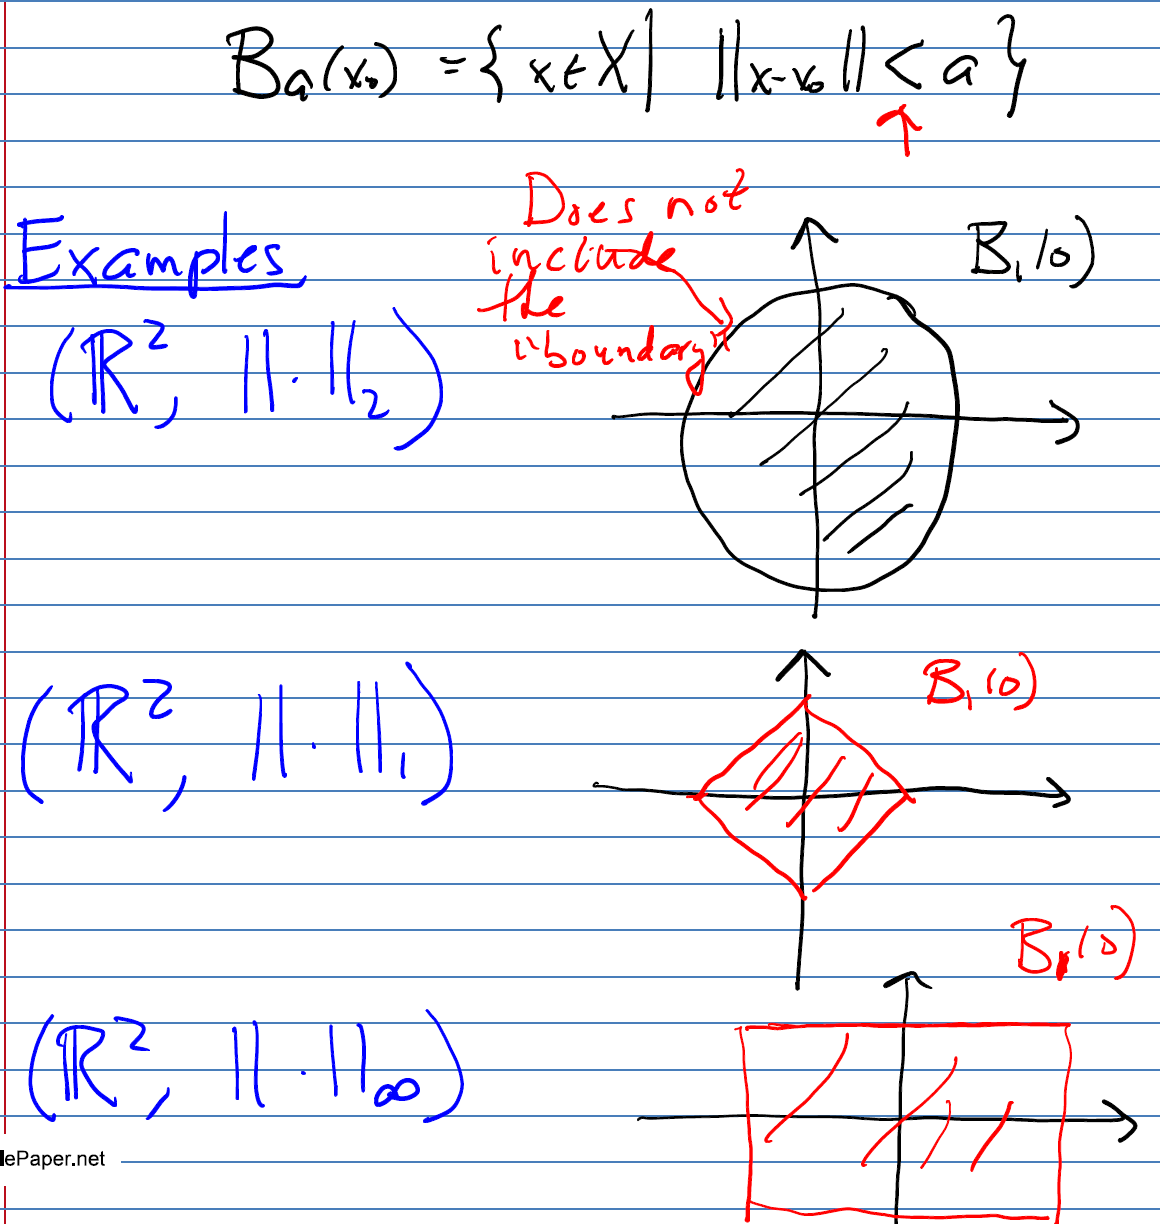
\includegraphics[width=0.7\columnwidth]{graphics/Chap06/UnitBalls.png} }
    \caption[]{ $\left(\real^2,\ \|\bullet\|\right)$ with various norms: (a) Euclidean norm $\|(x_1,\ x_2)\|_2=\sqrt{|x_1|^2+|x_2|^2 }$; (b) One norm  $\|(x_1,\ x_2)\|_1=|x_1|+|x_2|$; and (c) Max norm $ \|(x_1,\ x_2)\|_\infty=\max_{1\leq i\leq 2}|x_i|$. }
    \label{fig:UnitBalls}
\end{figure} 


\begin{lem}\textbnf{(Characterization of distance zero and greater than zero)} Let $\left(\mathcal{X},\ \| \bullet \|\right)$ be a normed space, $x\in\mathcal{X}$, and $S\subset\mathcal{X}$. Then,
    \begin{align*}
        d(x,\ S)=0 &\iff \forall\epsilon>0,\ \exists y\in S,\ \|x-y\|<\epsilon ~~(\text{definition of  the infimum})\\
        &\iff \forall\epsilon>0,\ B_\epsilon(x)\cap S\neq \emptyset ~~(\text{definition of an open ball of radius} ~\epsilon). \text{ Moreover, } \\
        \\
        d(x,\ S)>0 &\iff \exists\epsilon>0,\ \forall y\in S,\ \|x-y\|\geq\epsilon\\
        &\iff \exists\epsilon>0 \textnormal{ such that } B_\epsilon(x)\cap S = \emptyset\\
        &\iff  \exists\epsilon>0 \textnormal{ such that } B_\epsilon(x)\subset (\sim S).
    \end{align*}
\end{lem} 

\begin{figure}[hbt!]%
    \label{fig:DistanceZero2aSet}
\centering{
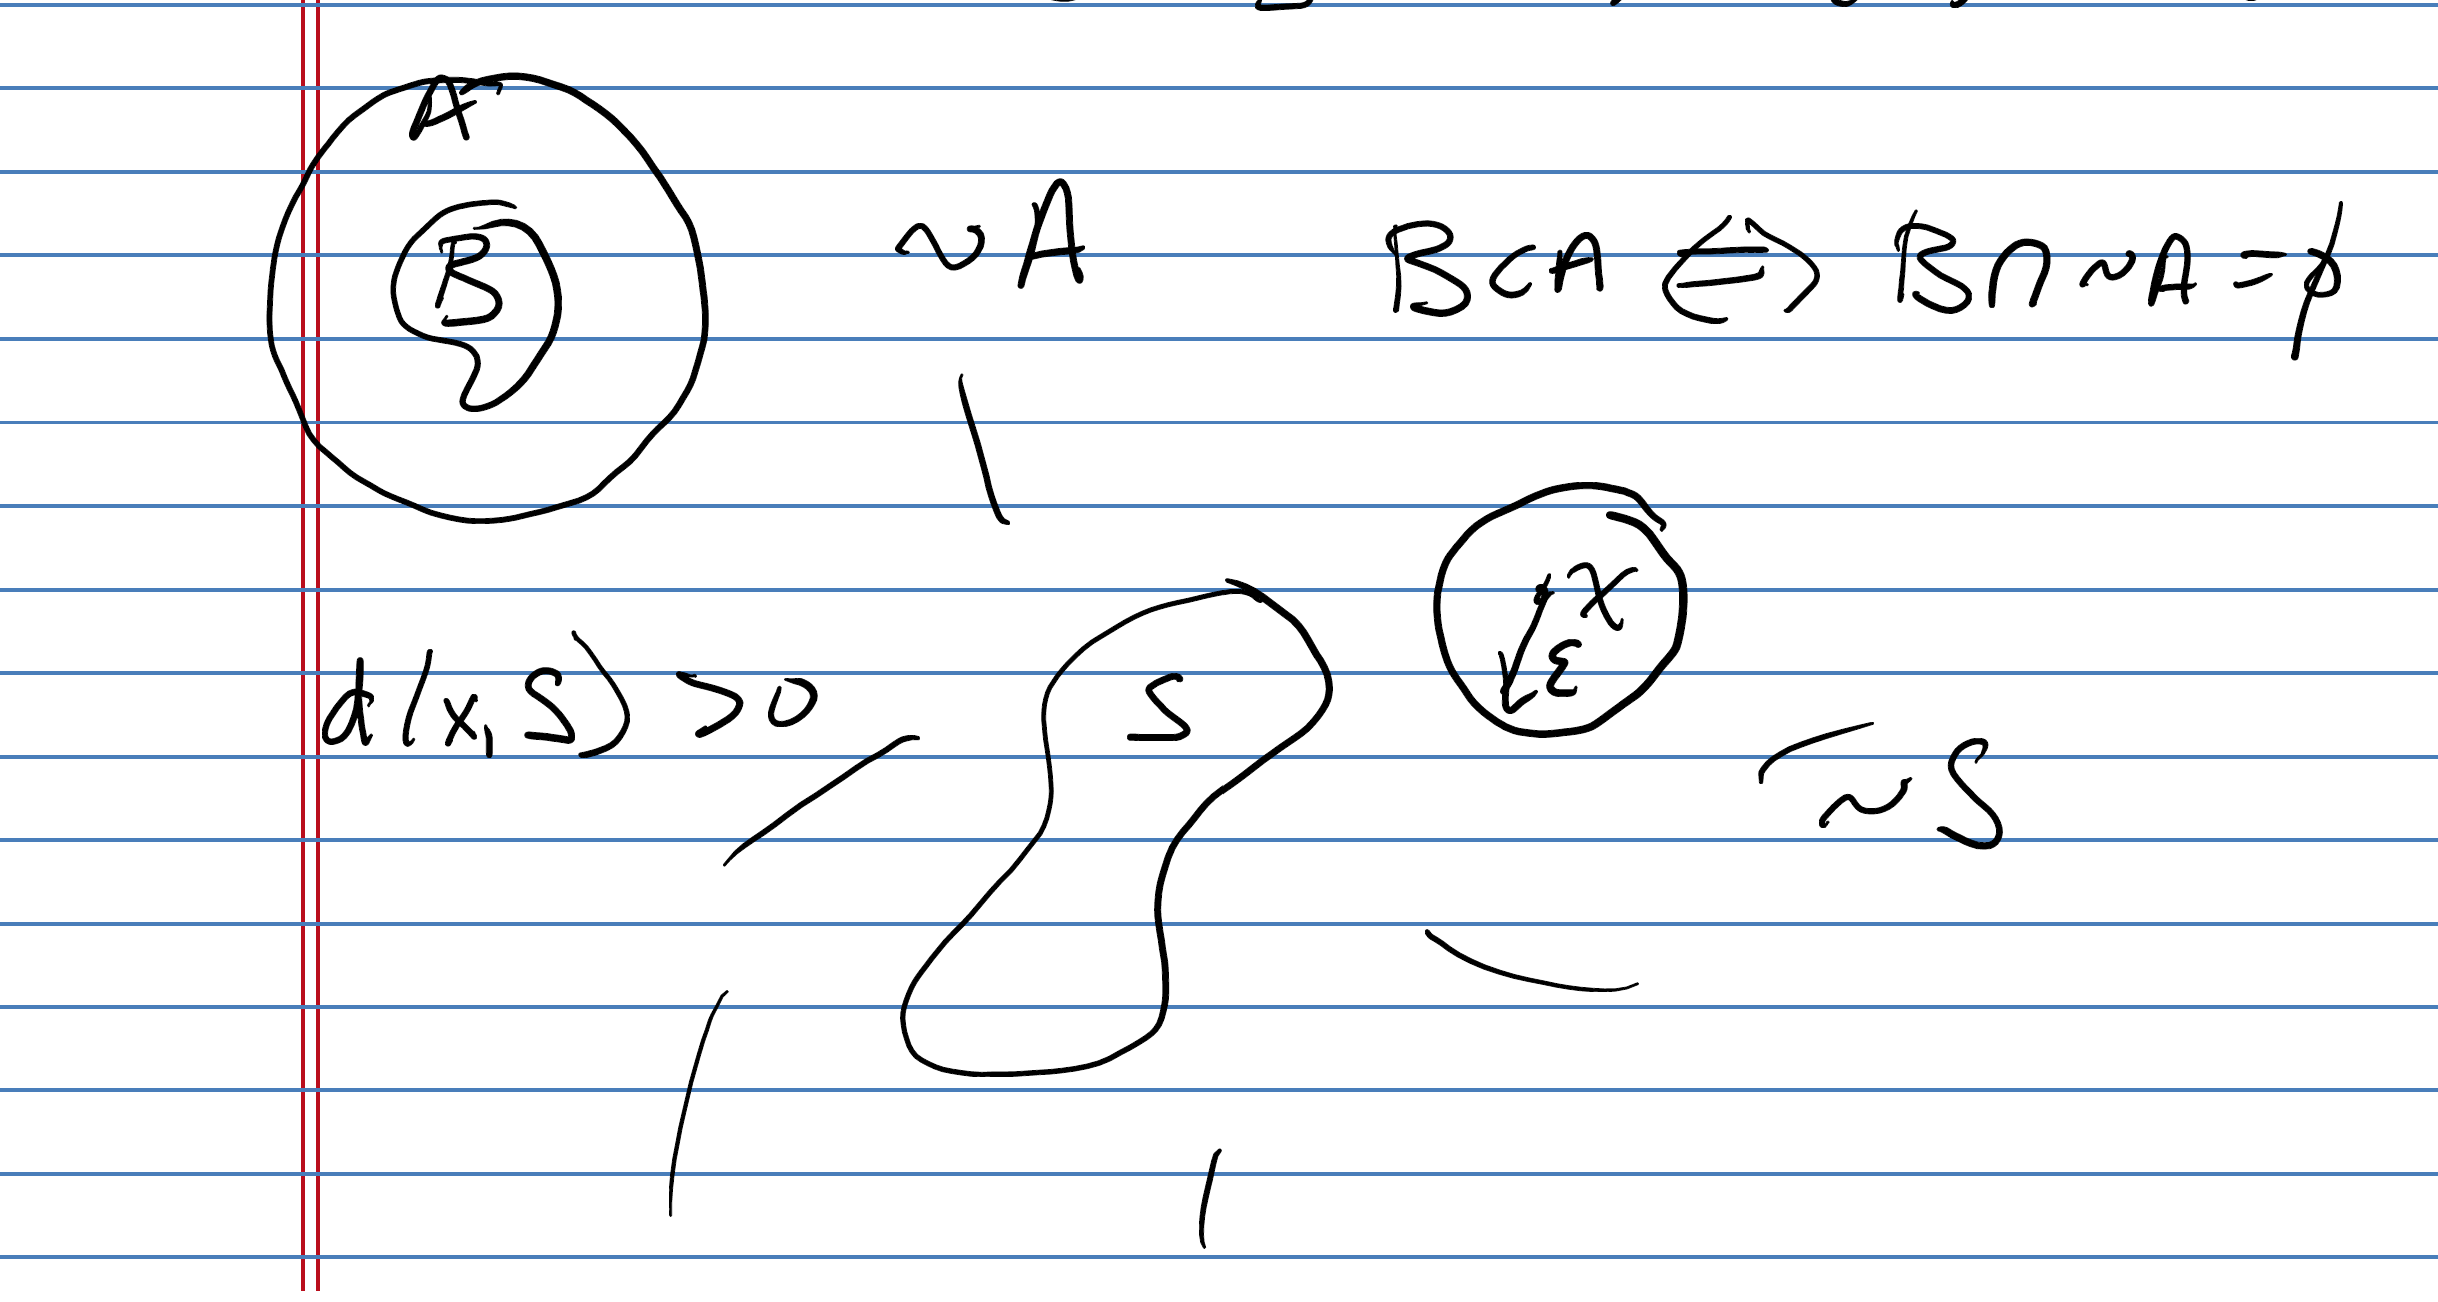
\includegraphics[width=0.7\columnwidth]{graphics/Chap06/DistancextoSpositive.png} 
}
\caption[]{ Why $(d(x, S)>0) \iff (\exists ~\epsilon>0$ such that $ B_\epsilon(x) \subset (\sim S)) \iff (\exists ~\epsilon>0$ such that $ B_\epsilon(x) \cap S = \emptyset)$. We simply take $\epsilon = \frac{d(x, S)}{2} >0.$ }
\end{figure} 


 In the following, we assume $\left(\mathcal{X},\ \| \bullet \|\right)$ is given.
 
\begin{definition} Let $P\subset\mathcal{X}$, a subset of $\mathcal{X}$. 
    \begin{enumerate}
          \renewcommand{\labelenumi}{(\alph{enumi})}
        \setlength{\itemsep}{.1cm} 
        \item A point $p\in P$ is \textbf{ an interior point of $P$} if $\exists\epsilon>0$ such that $B_\epsilon(p)\subset P$.
        \item The \textbf{interior of $P$} is $\mathring{P}:=\{p\in P\ |\ p\textnormal{ is an interior point}\}$.
            \end{enumerate}
\end{definition}

\begin{rem} \mbox{ }
\begin{align*}
    \mathring{P} & = \{ p \in P~ |~ \exists \epsilon >0, B_\epsilon(p) \subset P\} \\
        & = \{ p \in P~ |~ d(p, \sim P) >0\} \\
        & =  \{ x \in \mathcal{X}~ |~ d(x, \sim P) >0\}
\end{align*}
because if $x \in (\sim P)$, then $d(x, \sim P)=0$ and $\mathcal{X} = P \cup (\sim P)$. Hence, 
\begin{center}
 $$ \boxed{\mathring{P} = \{ x \in \mathcal{X}~|~ d(x, \sim P) > 0 \}.}$$
\end{center}
\end{rem}

\begin{definition} $P$ is \textbf{open} if $\mathring{P} =P$.
\end{definition}

\begin{rem} Hence, $P$ is open if, and only if, $P= \{ x \in \mathcal{X}~|~ d(x, \sim P) > 0 \}$.

\end{rem}
    

\begin{example} Checking if sets are open or not.
\begin{itemize}
        \item Is $P=(0,\ 1)\subset(\real,\ \| \bullet \|)$ open? We note that $(x \in P \implies  0 < x < 1)$ and define $\epsilon = \min\{\frac{x}{2}, \frac{1-x}{2}\} $. Then $B_\epsilon(x) \subset P$ and hence $P$ is open.\\
        
        \item  Is $P=(0,\ 1)\subset(\real,\ \| \bullet \|)$ open? We check it a second  way. $\sim P = (-\infty, 0] \cup [1, \infty)$. We have $x \in P \iff 0 < x < 1$. Hence, 
        \begin{align*}
                d(x, (-\infty, 0])&=x>0\\
                d(x,  [1, \infty))&=1-x>0\\
                d(x, \sim P) &= \min\{x, 1-x\} > 0.
        \end{align*}
            Hence, $x \in P \iff d(x, \sim P) >0$, and thus $P$ is open.
        \item $P=[0,\ 1)\subset(\real,\ |  \bullet |)$ is not open because $0\in P$, and $\forall\epsilon>0$, $B_\epsilon(0)\cap(\sim P)\neq\emptyset$ or we can also check it's not open because $0\in P$ and $d(0, \sim P)=0$.
    \end{itemize}

    
\end{example}
    
\begin{definition} $P\subset \mathcal{X}$ a subset.
\begin{enumerate}
        \item A point $x\in \mathcal{X}$ is a \textbf{closure point} of $P$ if $\forall\epsilon>0$, $\exists p\in P$ such that $\|x-p\|<\epsilon$, in other words,  $d(x, P)=0$.
        \item The \textbf{closure of} $P$ is $\overline{P}:=\{x\in\mathcal{X} ~|~ x \text{ is a closure point}\}$
    \end{enumerate}
\end{definition}

\begin{definition}  $P$ is \textbf{closed} if $\overline{P}=P$.

\end{definition}
    

\begin{example} Consider $(\mathcal{X}, \| \bullet \|) = (\real,| \bullet |). $
    \begin{enumerate}
    \item $P=[0,\ 1)$ is not closed because $1 \not \in P$, and $d(1,P)=0$.
    \item $P=[0,\ 1]$ is closed because $x \not \in P$ implies $d(x, P)=\max\{-x, x-1  \} >0$.
        \item $P=(0,\ 1)\implies \overline{P}=[0,\ 1]$ because $d(0, P)=0$, $d(1, P)=0$ and for $x\not \in [0, 1], d(x, P)>0$.
    \end{enumerate}
\end{example}

\begin{fact} The rational numbers $\mathcal{Q} \subset \real$ are neither closed nor open. $\overline{\mathcal{Q}}=\real$.
    
\end{fact}
    


\begin{thm} \textbf{(Characterization of Open and Closed Sets using Distance)} Let $(\mathcal{X}, \| \bullet \|) $ be a normed space and $P\subset \mathcal{X}$ a subset. Then $P$ is open if, and only if, $\sim P$ is closed. \\
\begin{center}
\boxed{
\begin{aligned}
        P\textnormal{ is closed}&\iff\ \sim P\textnormal{ is open}.\\
        P\textnormal{ is open} &\iff\ \sim P\textnormal{ is closed}.
    \end{aligned}
}
\end{center}
  \end{thm}
   

\textbf{Proof:} The proof can be given in one line.
$$\boxed{
    \underbrace{\sim P=\sim(\mathring{P})}_{P\textnormal{ is open}}=\{x\in\mathcal{X}\ |\ d(x,\ \sim P)=0\}=\underbrace{\overline{\sim P}=\sim P}_{\sim P\textnormal{ is closed}}
    }
$$
We'll unpack it for you. 

\begin{align*}
    P = \mathring{P} & \iff P = \{ x \in \mathcal{X}~|~ d(x, \sim P) > 0 \}\\
                        & \iff P = \{ x \in \mathcal{X}~|~\exists \epsilon >0, B_\epsilon(x) \cap P = \emptyset\}\\
                      &  \iff P = \sim \{ x \in \mathcal{X}~|~\forall \epsilon >0, B_\epsilon(x) \cap P \neq \emptyset\}\\
                       &  \iff \sim P = \{ x \in \mathcal{X}~|~\forall \epsilon >0, B_\epsilon(x) \cap P \neq \emptyset\}\\
                       &  \iff \sim P = \{ x \in \mathcal{X}~|~d(x, \sim P) = 0\}\\
                       &  \iff \sim P = \overline{\sim P}
\end{align*}
Hence, $P = \mathring{P} \iff \sim P = \overline{\sim P}$, so $P$ is open if, and only if, $\sim P$ is closed. 
\Qed
 \begin{rem} Can a set be both open and closed? Yes. Such sets are sometimes called \textbf{clopen}! If $(\mathcal{X}, \| \bullet \|)$ is a normed space, then $\mathcal{X}$ is both open and closed. By convention,the empty set $\emptyset$ is both open and closed (Why? For two reasons: (i) Because it does not violate the conditions to be open or closed. (ii) We want the set complement of an open set to be a closed set and vice versa). 
 \end{rem}
 
 \begin{exercise} Show the following:
 \begin{enumerate}
    \renewcommand{\labelenumi}{(\alph{enumi})}
        \setlength{\itemsep}{.1cm}
     \item An arbitrary union of open sets is open.
     \item A arbitrary intersection of closed sets is closed.
     \item A finite intersection of open sets is open.
     \item A finite union of closed sets is closed.
 \end{enumerate}
 \end{exercise}
 
  
 \begin{example} Consider the real numbers as a normed space; that is,  ${\cal X} = \real$ and define the norm to be $||x|| = |x|$, the standard absolute value. Is the infinite intersection of open sets $$ \bigcap\limits_{n=1}^{\infty} (-1- \frac{1}{n}, 1)    $$ open?
 \end{example}
 
 \textbf{Solution:} \textbf{No}. Indeed, $\forall~n\ge 1$, $[-1,1) \subset (-1- \frac{1}{n}, 1)$. Hence, by definition of the intersection, $[-1,1) \subset \bigcap\limits_{n=1}^{\infty} (-1- \frac{1}{n}, 1)$. Moreover, $$[-1,1) = \bigcap\limits_{n=1}^{\infty} (-1- \frac{1}{n}, 1), $$
      because if $x<-1$, then there exits $1\le K<\infty$ such that $x < -1-\frac{1}{K}$, which implies that $x\not \in  (-1- \frac{1}{K}, 1)$, and thus
      $$ x \not \in \bigcap\limits_{n=1}^{\infty} (-1- \frac{1}{n}, 1). $$
      
\Qed
 
 \begin{exercise} Show the following:
  \begin{enumerate}
     \renewcommand{\labelenumi}{(\alph{enumi})}
        \setlength{\itemsep}{.1cm}
     \item $P$ is closed if, and only if, $\overline{P} \subset P$.
     \item $P$ is open if, and only if, $ P \subset \mathring{P}$.
 \end{enumerate}
 
 \end{exercise} 
 
 \begin{definition} The \textbf{boundary} of $S \subset \mathcal{X}$ is $\partial S:= \overline{S} \cap \overline{(\sim S)}.$
 \end{definition}
 
 \begin{exercise} Show that $\partial S= \overline{S} \setminus \mathring{S} := \{ x \in \overline{S}~|~ x \not \in \mathring{S}\}$.
 
 \end{exercise}

\section{Newton-Raphson Algorithm}

As Roboticists and Engineers, we are often faced with problems for which closed-form solutions are unknown or do not exist. For such problems, we often seek iterative means to either compute a solution or to prove the existence of a solution. \\

Consider a function $f:\real^n \to \real^n$ that is continuously differentiable and suppose we seek a root $f(x^\ast)=0$. Note that the domain and range are both $\real^n$ and thus this is the nonlinear equivalent of solving a square linear equation $Ax-b=0$.\\

The \textbf{Newton-Raphson} Algorithm is a vector version of Newton's Algorithm; see Chapter 11 of the ROB 101 Textbook. Let $x_k \in \real^n$ be our current approximation of a root of the function $f$. We write the linear approximation of $f$ about the point $x_k$ as
\begin{equation}
    \label{eq:NewtonMethodVector01}
    f(x) \approx f(x_k) + \frac{\partial f(x_k)}{\partial x}\cdot (x - x_k).
\end{equation}
We want to chose $x_{k+1}$ so that $f(x_{k+1})=0$, but we cannot do that exactly. Based on the linear approximation in \eqref{eq:NewtonMethodVector01}, we have that 
\begin{equation}
    \label{eq:BasicNewtonRaphson}
     f(x_{k+1}) \approx 0 \iff  0  \approx f(x_k) + \frac{\partial f(x_k)}{\partial x}\cdot (x_{k+1} - x_k).
\end{equation}
If $\det\left(\frac{\partial f(x_k)}{\partial x} \right)\neq 0$, we can solve for $x_{k+1}$, giving us the standard form of the Newton-Raphson Algorithm, 
$$ \boxed{    x_{k+1}=x_{k} - \left(   \frac{\partial f(x_k)}{\partial x}\right)^{-1} f(x_k).}$$


The ``hope'' is that each iteration of the algorithm produces a better approximation $x_k$ to a root of the function $f(x)$, where by a better approximation, we mean that if $x^\ast$ is an unknown root of $f$, then in the limit as $k$ gets sufficiently large, we can make $\|x^\ast - x_k\|$ arbitrarily small. We formalize these ideas in Chapter~\ref{sec:sequences} with the notion of a converging sequence and in Chapter~\ref{sec:Contraction} on Contraction Mappings. For now, we'll simply see a numerical illustration of these ideas in action.

\vspace*{0.2cm}
\begin{tcolorbox}[title=\textbf{Alternative Form of the Newton-Raphson Algorithm}]
Based on \eqref{eq:BasicNewtonRaphson}, we define\footnote{Note that $\Delta x_k = x_{k+1}-x_k$.} $x_{k+1}:= x_k + \Delta x_k$, where $ \Delta x_k$ is our update to $x_k$. We can then break the algorithm into two steps,
\begin{align}
\label{eq:NewtonRaphsonStep1}
\left(\frac{\partial f(x_k)}{\partial x} \right) \Delta x_{k} &= - f(x_k) \hspace*{0.58cm}(\text{solve for}~~\Delta x_k)  \\
\label{eq:NewtonRaphsonStep2}
x_{k+1}&= x_k + \Delta x_{k}~~(\text{use~~} \Delta x_k ~~\text{to update our estimate of the root}).
\end{align}
While for toy problems, we can use the matrix inverse to solve \eqref{eq:NewtonRaphsonStep1} for $\Delta x_{k}$, for larger problems, we recommend using an LU Factorization or a QR Factorization. Once \eqref{eq:NewtonRaphsonStep1}  has been solved, $x_{k+1}$ is updated in \eqref{eq:NewtonRaphsonStep2} and the process repeats.\\

A \textbf{damped Newton-Raphson Algorithm} is obtained by replacing \eqref{eq:NewtonRaphsonStep2} with   
\begin{equation}
    \label{eq:NewtonRaphsonStep3}
x_{k+1}= x_k + \epsilon \Delta x_{k},
\end{equation}
for some $\epsilon >0$.
 The validity of the Newton-Raphson Algorithm rests upon: 
\begin{itemize}
    \item the function $f$ being differentiable;
    \item the Jacobian $\frac{\partial f(x_k)}{ \partial x}$ having a non-zero determinant at points generated by \eqref{eq:NewtonRaphsonStep1} and \eqref{eq:NewtonRaphsonStep2}; and
    \item the linear equation $f_{\rm lin}(x) = f(x_k) + \frac{\partial f(x_k)}{ \partial x} (x - x_k) $ being a good approximation to the function.
\end{itemize}
\end{tcolorbox}
    

\begin{example}
\label{ex:NewtonRaphson}
Find a root of $F:\real^4 \to \real^4$ near $x_0=\left[\begin{array}{cccc} -2.0 & 3.0 & \pi &-1.0\end{array} \right]$ for
$$
F(x)=\left[\begin{array}{c}
   x_1 + 2 x_2 - x_1 (x_1 + 4 x_2) - x_2 (4 x_1 + 10 x_2) + 3 \medskip \\
 3 x_1 + 4 x_2 - x_1 (x_1 + 4 x_2) - x_2 (4 x_1 + 10 x_2) + 4  \medskip\\
                                0.5 \cos(x_1) + x_3 -\left( \sin(x_3) \right)^7  \medskip\\
                              -  2(x_2)^2  \sin(x_1) + (x_4)^3
\end{array} \right].
$$

\end{example}

\textbf{Solution:} We programmed up \eqref{eq:NewtonRaphsonStep1} and \eqref{eq:NewtonRaphsonStep2} in Julia and used a symmetric difference approximation for the derivatives, with $h=0.1$. Below are the first five results from the algorithm:
$$
x_k = \left[
\begin{array}{rrrrrr}
k=0~~ & k=1~~ & k=2 ~~& k=3~~ & k=4~~& k=5~~ \medskip \\
-2.0000 & -3.0435 & -2.4233 & -2.2702 & -2.2596 & -2.2596 \\
3.0000 & 2.5435 & 1.9233 & 1.7702 & 1.7596 & 1.7596 \\
3.1416 & 0.6817 & 0.4104 & 0.3251 & 0.3181 & 0.3181 \\
-1.0000 & -1.8580 & -2.0710 & -1.7652 & -1.6884 & -1.6846 
\end{array}
\right]
$$
and
$$
f(x_k) = 
\left[
\begin{array}{rrrrrr}
k=0~~ & k=1~~ & k=2 ~~& k=3~~ & k=4~~& k=5~~ \medskip\\
-39.0000 & -6.9839 & -1.1539 & -0.0703 & -0.0003 & -0.0000 \\
-36.0000 & -6.9839 & -1.1539 & -0.0703 & -0.0003 & -0.0000 \\
2.9335 & 0.1447 & 0.0323 & 0.0028 & 0.0000 & -0.0000 \\
15.3674 & -5.1471 & -4.0134 & -0.7044 & -0.0321 & -0.0001
\end{array}
\right].
$$
By iteration five, we have a good approximation of a root because $||f(x_5)|| \approx 10^{-4}$.
To emphasize that as $x_k$ evolves, so does the Jacobian of $f$ at $x_k$, we provide the Jacobians at the initial and final steps,
$$
 \frac{\partial f(x_0)}{\partial x}=\left[
\begin{array}{rrrr}
-19.0000 & -42.0000 & 0.0000 & 0.0000 \\
-17.0000 & -40.0000 & 0.0000 & 0.0000 \\
0.4539 & 0.0000 & 1.0000 & 0.0000 \\
7.4782 & 10.9116 & 0.0000 & 3.0100 \\
\end{array}
\right] \text{~~and~~}  \frac{\partial f(x_5)}{\partial x} = 
\left[
\begin{array}{rrrr}
-8.5577 & -15.1155 & 0.0000 & 0.0000 \\
-6.5577 & -13.1155 & 0.0000 & 0.0000 \\
0.3854 & 0.0000 & 0.9910 & 0.0000 \\
3.9296 & 5.4337 & 0.0000 & 8.5616 \\
\end{array}
\right].
$$

\Qed




Hopefully, you now have in your mind that iteration is useful. We formalize the process of doing iterations through sequences of vectors in normed spaces.

\section{Sequences}
\label{sec:sequences}

Once again, we let $(\mathcal{X}, \| \bullet\|)$ be a normed space. 

\begin{definition} A set of vectors indexed by the non-negative integers is called a \textbf{ sequence}. Common notion includes $(x_n)$ or $\{x_n\}$. 
\end{definition}

\begin{definition} A sequence of vectors $(x_n)$ \textbf{ converges} to $x\in \mathcal{X}$ if, $\forall$ ${\epsilon} > 0,\ {\exists} N({\epsilon}) < {\infty}$ such that, $n{\geq}N \implies \|x_n-x\| < \epsilon$, i.e., $n {\geq}N\to \ x_n {\in} B_{\epsilon}(x).$ One writes
    \begin{equation*}
        \lim\limits_{n \to \infty} x_n= x\textnormal{ or }x_n \to  x\textnormal{ or }x_n  \xrightarrow[n \to \infty]{} x.
    \end{equation*}

\end{definition}

\begin{prop} Suppose $x_n \to x $. Then,
    \begin{enumerate}
       \renewcommand{\labelenumi}{(\alph{enumi})}
        \setlength{\itemsep}{.1cm}
        \item $\| x_n \| \to \| x \|$
        \item $\sup\limits_{n}\| x_n \| < \infty$ (The sequence is bounded.)
        \item If $x_n \to y$ then y = x. (Limits are unique.)
    \end{enumerate}
    
\end{prop} 

\begin{rem} 
\label{rem:HandyInequality}
(Handy Inequality) For $\overline{x},\ \overline{y}\in \mathcal{X},$
    \begin{align*}
 \| \overline{x} \| &= \| \overline{x}-\overline{y}+\overline{y} \| \\
 &\leq \| \overline{x}-\overline{y} \| + \| \overline{y} \|\\
 &\Downarrow \\
  \| \overline{x} \| -\| \overline{y} \| &\leq \| \overline{x}-\overline{y} \|
    \end{align*}
    The same argument shows that $ \| \overline{y} \| -\| \overline{x} \| \leq \| \overline{x}-\overline{y} \|$. Hence
    $$\boxed{ | ~\| \overline{x} \| - \| \overline{y} \| ~|  \leq \| \overline{x}-\overline{y}\|.}$$
    $\hfill \square$

\end{rem}

\textbf{Proof of the Proposition:}
    \begin{enumerate}
        \item From Remark~\ref{rem:HandyInequality}, $|~ \| x \| - \| x_n\| ~| \leq \| x-x_n\|$ $\xrightarrow[n \to \infty]{}$ 0.
        \item Applying the definition of convergence of a sequence, we set $\epsilon = 1$ and deduce  $\exists N(1) <\infty$ such that $n \geq N \implies  \|x_n-x\| \leq 1$. Hence,  $\forall n \geq N,\ \| x_n\| =\|x_n-x+x\| \leq \| x_n - x\| + \| x \| \leq 1+\| x \|.$ It follows that
            \begin{equation*}
                \sup\limits_{k}\| x_k\| \leq \operatorname{max}\{\underbrace{\| x_1\|, \| x_2\|, \dotsb , \| x_{N-1}\|, 1+ \| x \|}_\textnormal{finite}\}<\infty.
            \end{equation*}
        \item $\| x-y\| = \| x-x_n +x_n-y\| \leq \| x-x_n\| + \| x_n -y\| \xrightarrow[n \to \infty]{} 0  \implies x=y$.
    \end{enumerate}
    \Qed

\begin{definition} Let $x\in \mathcal{X}$, $P \subset \mathcal{X}$ a subset. 
\begin{enumerate}
    \item $x$ is a \textbf{ limit point} of $P$ if there exists a non-trivial sequence of elements of $P$ that converges to $x$. That is, $\exists (x_n)$, such that for all $n\ge 1$,  $x_n \in P$, $x_n \neq x$ and $\lim\limits_{n \to \infty} x_n = x.$ Here, non-trivial means that you cannot create the sequence $(x_n=x)$.
    \item If $x\in P$ is not a limit point of $P$, then $x$ is called an \textbf{isolated point of $P$}.
\end{enumerate}
\end{definition} 

\begin{prop} \textbf{(Characterization of Isolated Points)} $x$ is an isolated point of $P$ if, and only if, there exists $\epsilon>0$ such that $B_\epsilon(x) \cap P = \{ x\}$.
\end{prop}

\textbf{Proof:} Suppose there exists $\epsilon>0$ such that $B_\epsilon(x) \cap P = \{ x\}$, and let $(x_n)$ be such that for all $n\ge 1$,  $x_n \in P$ and $x_n \neq x$. Then, for all $n\ge 1$, $d(x_n, x)\ge \epsilon$ and hence $x_n \not \to x$. For the other direction, we suppose that $\forall \epsilon>0$, $B_\epsilon(x) \cap P \neq \{ x\}$. Since $x\in B_\epsilon(x) \cap P$, we deduce that for all $\epsilon=1/n$, there exists $x_n\neq x$ and $x_n\in B_\epsilon(x) \cap P$. Hence $x$ satisfies all conditions of a limit point, namely $x_n\in P$, $x_n \neq x$, and $\lim_{n \to \infty} x_n = x$.
\Qed

\begin{rem}
    Let$x$ be an isolated point of $P$. Then $x$ is an element of $P$ and the trivial sequence $(x_n=x) \to x$. Moreover, if $(x_n)$ is a sequence of elements in $P$ and $\lim_{n \to \infty} x_n = x$, then there exists $N <\infty$ such that, for all $n \ge N$, $x_n = x$. In other words, the ``tail'' of the sequence is a trivial sequence. 
\end{rem}

\begin{prop} \textbf{(Characterization of Set Closure using Limit Points and Isolated Points)}
\label{prop:closureANdLimitPoings} 
Let $P_{\rm iso}$ be the collection of all isolated points of $P$ and let $P_{\infty}$ be the collection of all limit points of $P$. Then $$\overline{P} = P_{\rm iso} \cup P_{\infty}.$$
\end{prop} 

\textbf{Proof:} 
    \begin{enumerate}
        \item Suppose $x$ is a limit point or an isolated point. Then, $\exists (x_n)$ such that $x_n\in P$ and $x_n\to x$. Because $x_n\to x$, $\forall \epsilon>0$, $\exists x_n\in P$ such that $\|x_n-x\|<\epsilon$, which implies that $d(x,\ P)=0$. Hence $x\in\overline{P}$.
        \item Suppose $x\in\overline{P}$. Then, $d(x, P)=0$ and hence, for all $n\ge 1$, $B_{ \frac{1}{n} } (x) \cap P \neq \emptyset$. Two cases are possible. For some $N < \infty$, and all $N\ge N$, $B_{ \frac{1}{n} } (x) \cap P =\{x\}$, in which case, $x \in P_{\rm iso}$. Otherwise, for $n\ge 1$, there exists $x_n\in B_{ \frac{1}{n} } (x) \cap P$ such that $x_n \neq x$, in which case, the sequence $(x_n)$ establishes that $x \in  P_{\infty}$.
    \end{enumerate}

\begin{cor}
\label{cor:ClosureAndLimitPoints}
$P$ is closed if, and only if,  it contains its limit points, that is, $$\overline{P}=P \iff P_\infty \subset P. $$
\end{cor} 

% 
\textbf{Proof:} By definition, $P_{\rm iso} \subset P$. Hence, if  $P_\infty \subset P$, then $P_{\rm iso} \cup P_{\infty} \subset P$, which implies by Proposition~\ref{prop:closureANdLimitPoings} that $\overline{P} \subset P$, and hence $P$ is closed. For the other direction, if $P$ is closed, then Proposition~\ref{prop:closureANdLimitPoings} implies that $P_\infty \subset P$, and hence the proof is done. 
\Qed. 

\section{Cauchy Sequences and Completeness}

In practice, the definition of a convergent sequence is hard to apply because, to check it, you must have a ``guess'' of what the limit actually is! This led the mathematician Augustin-Louis Cauchy to propose a a related property, that now bears his name \url{https://en.wikipedia.org/wiki/Cauchy_sequence}.\\ 

\begin{definition}
A sequence $(x_n)$ is \textbf{Cauchy} if $\forall~\epsilon >0$  $\exists N(\epsilon) <\infty$, such that $n \geq N$ and $ m \geq N$ $\implies \| x_n - x_m\| < \epsilon$.
\end{definition}

\begin{notation} We'll denote $(x_n)$ is Cauchy by $\|x_n-x_m\|\xrightarrow[n,\ m ~\to \infty]{}0$

\end{notation} 

The following captures the idea of terms in a sequence getting closer and closer together. The analysis will prepare us for the Contraction Mapping Theorem.

\begin{lem} Let $0 \le c <1$ and let $(a_n)$ be a sequence of real numbers satisfying, $\forall~n\ge 1$,
 $$|\ak{n+1}-\ak{n}| \le c | \ak{n}-\ak{n-1}|. $$
 Then $(a_n)$ is Cauchy in $(\real, | \bullet |)$.
\end{lem}

\textbf{Proof:}\\

\ul{Step 1:}  $\forall ~n\ge 1$, $|\ak{n+1}-\ak{n}| \le c^n |a_1-a_0|$.\\

\textbf{Pf:} First observe that $|\ak{3}-\ak{2}|\le c|\ak{2}-\ak{1}| \le c^2|a_1-a_0|$ and then complete the proof by induction. 

$\hfill \square$

\ul{Step 2:} $\forall ~n\ge 1, k \ge 1$, $|\ak{n+k}-\ak{n}| \le \frac{c^n}{1-c} |a_1-a_0|$.\\

\textbf{Pf:}
\begin{align*}
|\ak{n+k}-\ak{n}| &\le | \ak{n+k}-\ak{n+k-1} + \ak{n+k-1}-\ak{n+k-2} +\cdots \ak{n+1}-\ak{n}| \\
&\le | \ak{n+k}-\ak{n+k-1}| + |\ak{n+k-1}-\ak{n+k-2}| +\cdots |\ak{n+1}-\ak{n}| \\
&\le c^{n+k-1}|a_1-a_0| + c^{n+k-2}|a_1-a_0| + \cdots + c^n |a_1-a_0|  \\
&\le c^n \left( \sum_{i=0}^{k-1} c^i \right)~ |a_1-a_0| \\
&\le c^n \left(\sum_{i=0}^{\infty} c^i \right)~ |a_1-a_0| \\
&\le c^n \left( \frac{1}{1-c} \right) ~ |a_1-a_0|\\
&\le  \frac{c^n }{1-c}~|a_1-a_0|.
\end{align*}
$\hfill \square$

\ul{Step 3:} $(a_n)$ is Cauchy.\\

\textbf{Pf:} Consider $m$ and $n$ and without loss of generality, suppose $m \ge n$. If $m=n$, then $|a_m-a_n|=0$. Thus, we can assume $m=n+k$ for some $k\ge1$. Then
$$|a_m-a_n|=|a_{n+k}-a_n|\le \frac{c^n}{1-c} |a_1-a_0| \xrightarrow[n\to \infty,~ m\ge n]0,$$
and thus $(a_n)$ is Cauchy.

$\hfill \square$

\Qed


\begin{prop} If $x_n\to x$, then $(x_n)$ is Cauchy.
\end{prop}


\textbf{Proof:} If  $x_n\to x$, then  $\forall ~\epsilon>0$ $\exists~ N<\infty$  such that $\forall ~ n\geq N$, $\|x_n-x\|<\frac{\epsilon}{2}$. Hence, if $m\ge N$    
\begin{align*}
            \| x_n - x_m \| &= \| x_n - x + x - x_m \|\\
            &\leq \| x_n - x \| + \| x- x_m \|\\
            &< \frac{\epsilon}{2} + \frac{\epsilon}{2}\\
            &< \epsilon\ \ \ \ \ \textnormal{for all }n,\ m\geq N
        \end{align*}
\Qed    
    
Unfortunately, not all Cauchy sequences are convergent. For a reason we will understand shortly, all counter examples are infinite dimensional.

\begin{figure}[htb]
    \centering{
        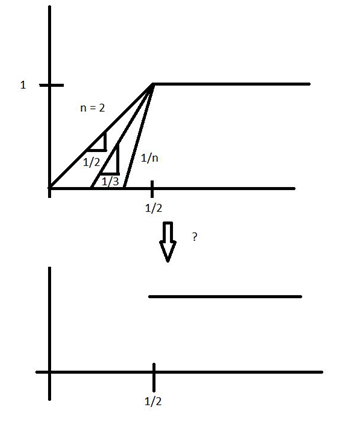
\includegraphics{graphics/Chap06/typeset.png}
        }
\caption[]{Visually, the sequence of continuous functions $(f_n(t))_{n=2}^\infty$ appears to be converging to a step function, which is discontinuous. If that is true, we then have a Cauchy sequence in $(\mathcal{X}, \| \bullet \|_1)$ that does not have a limit in the set $\mathcal{X}$. }
    \label{fig:NonConvergentCauchySequence}
    \end{figure}

\begin{example} Let $ \mathcal{X} :=  \{f:[0,1] \to \real \ \vert \ \textnormal{f is continuous}\}$ and equip it with the one-norm, $ \| f \|_1 := \int_0^1 \vert f(\tau)\vert d\tau$. Define a sequence as follow, where each function piecewise  is linear and $n \ge 2$,
    $$f_n(t)=\begin{cases}
        0 & 0\leq t\leq\frac{1}{2}-\frac{1}{n}\\
        1+n(t-\frac{1}{2}) & \frac{1}{2}-\frac{1}{n}\leq t\leq\frac{1}{2}\\
        1 & t\geq\frac{1}{2}.
    \end{cases}
    $$
    \textbf{Show that the sequence is Cauchy and does not have a limit in $ \mathcal{X}$}.
 
 \end{example} 
 
 \textbf{Proof:}  You may want to check that each function is continuous at the breakpoints, $\frac{1}{2}-\frac{1}{n}$ and $\frac{1}{2}$. Moreover, by using the area under a triangle, you can show
    $\| f_n - f_m \|_1=\frac{1}{2}$  $|\frac{1}{n}- \frac{1}{m}|$ $\xrightarrow[n,\ m \to \infty]{ }0$, and thus the sequence is Cauchy. \\
    
    
How can we show that there does not exist any (continuous) function $f \in \mathcal{X}$ to which the sequence converges? We define 
 $$f_{\rm step}(t):= \begin{cases} 0 & 0 \le  t < \frac{1}{2} \\ 1 &  \frac{1}{2} \le t \le 1 \end{cases}$$
 and note that $f_{\rm step}$ is discontinuous and hence $f_{\rm step} \not \in \mathcal{X}$. Define $\mathcal{Y}:=\spanof{ \mathcal{X}, f_{\rm step}} \subset \{ f:[0, 1] : \real \}$, the vector space of all functions from the interval $[0, 1]$ to the real numbers. You can check that $\| \bullet \|_1$ is also a norm on $\mathcal{Y}$ and observe that $f\in \mathcal{Y}$ is continuous if, and only if, $f\in \mathcal{X}$. Finally, you can easily compute that
 $$\|f_n - f_{\rm step} \|_1=\frac{1}{2n},$$ 
 and hence, $f_n \to f_{\rm step}$. By uniqueness of limits, there does not exist a continuous function in $\mathcal{Y}$ to which the sequence converges, and thus the sequence does not have a limit in $\mathcal{X}$. 
 
 \Qed

The study of Cauchy sequences led mathematicians to wonder if it is possible to find normed spaces where all Cauchy sequences do have limits (within the given normed space), and moreover, if a normed space was ``deficient'' in the sense that it had Cauchy sequences without limit, could it be ``enlarged'' or ``completed'' to one where all Cauchy sequences do have limits. These are great questions!

\begin{definition} A normed space $(\mathcal{X},\real,\|\cdot\|)$ is \textbf{complete} if every Cauchy Sequence in $X$ has a limit in $X$. Such spaces are also called \textbf{ Banach spaces}.
\end{definition} 

The above definition can only be useful if a list of useful Banach spaces is known; see \url{https://en.wikipedia.org/wiki/Banach_space#Examples_2}.   In EECS562, you will use $\left(C\left[0,\ T\right],\ \| \bullet \|_\infty\right)$, the set of continuous functions with the infinity (or max) norm. The sequence in Fig.~\ref{fig:NonConvergentCauchySequence} is not a Cauchy sequence in $\left(C\left[0,\ T\right],\ \| \bullet \|_\infty\right)$; you might want to check that.

\begin{fact} For $a<b$, both finite, $(C\left[a,\ b\right]$, $\| \bullet \|_\infty)$ is complete where $C\left[a,\ b\right]=\left\{f:\left[a,\ b\right]\to\real\ |\ f\textnormal{ continuous}\right\}$. We showed above that $(C[a, b], ||\bullet||_1)$ is not complete.
\end{fact}


\begin{definition} A subset $S$ of a normed space is \textbf{ complete} if every Cauchy Sequence in $S$ has a limit in $S$.

\end{definition} 

\begin{rem} $S$ is complete implies that $S$ is closed.
    
\end{rem}

\begin{thm} Let $(\mathcal{X}, || \bullet ||)$ be a normed space. Then,

\begin{enumerate} 
       \renewcommand{\labelenumi}{(\alph{enumi})}
        \setlength{\itemsep}{.1cm}
        \item Every finite dimensional subspace is complete.
        \item Any closed subset of a complete set is also complete.
    \end{enumerate}
\end{thm}

\begin{fact} Every normed space $(\mathcal{X}, || \bullet ||_X)$ has a \textbf{``completion''}. A bit loosely stated, this means there is a complete normed space $(\mathcal{Y}, || \bullet ||_Y)$ such that
\begin{enumerate}
       \renewcommand{\labelenumi}{(\alph{enumi})}
        \setlength{\itemsep}{.1cm}
    \item $\mathcal{X} \subset \mathcal{Y}$ ($\mathcal{X}$ can naturally be viewed as a subset of $\mathcal{Y}$. The precise definition involves isometric isomorphisms.)
    \item $\forall x\in \mathcal{X}$, $||x||_Y = ||x||_X.$ 
    \item $\overline{\mathcal{X}} = \mathcal{Y}$ ($\overline{\mathcal{X}}$ is the closure of $\mathcal{X}$ in $\mathcal{Y}$. Hence, $\mathcal{X}$ fits ``tightly'' into $\mathcal{Y}$ in that sense that for any point in $y \in \mathcal{Y}$, $d(y, \mathcal{X})=0$).
    \item $\mathcal{Y}$ = $\mathcal{X} \cup\{ \text{limit points of Cauchy sequences in } \mathcal{X}\}$
\end{enumerate}

\end{fact}

You might ask about the completion of $C[a,b]$ when the $||\bullet||_1$ is used? It turns out to be the set of Lebesgue integrable functions on $[0,1]$. We alluded to Lebesgue back in Chapter~\ref{sec:ProbableApology}.
    

\section{Contraction Mapping Theorem}
\label{sec:Contraction}

\begin{definition}
 Let $S \subset \mathcal{X}$ be a subset of a normed space $(\mathcal{X}, \| \bullet \|)$. A function $T : S \to S$ is a \textbf{ contraction mapping} if,
$ \exists ~0 \leq c < 1$ such that $\forall x,y \in S,$ 
$$ \|T\left(x\right)-T\left(y\right)  \| \leq c \|x-y\|.$$ 
A point $x^\ast \in S$ is a \textbf{fixed point} of $T$ if $T(x^\ast) = x^\ast$.
\end{definition}


\begin{thm}\textbf{(Contraction Mapping Theorem)} ~ If $T$ is a contraction mapping on a complete subset $S$ of a normed space $\left(\mathcal{X},\real,\| \bullet \|\right)$, then there exists a unique vector $x^\ast \in S$ such that $T\left(x^\ast\right) = x^\ast$. Moreover, for every initial point $x_0 \in S$, the sequence $x_{n+1} = T\left(x_n\right), n \geq 0$, is Cauchy, and $x_n \to x^\ast$.
\end{thm}

\textbf{ Proof:}~ Let $(x_n)$ be defined as in the statement of the theorem. Because $T$ is a contraction mapping, there exists $0 \le c < 1$ such that, for all $n\geq 1$,
    \begin{align*}
        \| x_{n+1}-x_n \| &= \| T\left(x_n\right)-T\left(x_{n-1}\right) \|\\
        &\leq c \| x_n-x_{n-1}\|
    \end{align*}
    
\begin{claim} $(x_n)$ is Cauchy and thus by the completeness of $S$, $\exists x^\ast \in S$ such that $x_n \to x^\ast$.
\end{claim} 

\textbf{Proof:} We leave as an exercise to show by induction that $\| x_{n+1}-x_n \| \leq c ^n\| x_1-x_0 \|$. Next, consider $\| x_m-x_n \|$, and without loss of generality, suppose $m=n+k,\ k > 0$. Then,
    \begin{align*}
        \| x_m-x_n \| &= \| x_{n+k}-x_n \|\\
        &= \| x_{n+k}-x_{n+k-1}+x_{n+k-1}- \dots +x_{n+1}-x_n\|\\
        &\leq \| x_{n+k}-x_{n+k-1}\|+ \dots + \| x_{n+1}-x_n\|\\
        &\leq \left(c ^{n+k-1}+c ^{n+k-2}+ \dots + c ^n\right)\|x_1-x_0\|\\
        &= c ^n \left( \sum\limits_{i=0}^{k-1} c ^i \right) \|x_1-x_0\|\\
        &\leq c ^n \left( \sum\limits_{i=0}^\infty c ^i \right)\|x_1-x_0\|\\
        &= \frac{c ^n}{1-c}\|x_1-x_0\| \xrightarrow[\substack{n\to \infty \\ m >n}]{}0
    \end{align*}
where we used a simple fact about the geometric series for $\frac{1}{1-c}$. Therefore, $\left(x_n\right)$ is Cauchy sequence in $S$, and by completeness, $\exists x^\ast \in S$ such that $x_n \to x^\ast$. 
$\hfill \square$

\begin{claim} $x^\ast=T\left(x^\ast\right)$ and thus $x^\ast$ is a fixed point of $T$.
\end{claim} 

\textbf{Proof:} Let $n\ge 1$ be arbitary. Then,
    \begin{align*}
        \| x^\ast-T\left(x^\ast\right) \| &= \| x^\ast-x_n+x_n- T\left(x^\ast\right)\| \\
        &=\| x^\ast-x_n+T\left(x_{n-1}\right)- T\left(x^\ast\right)\| \\
        &\leq \| x^\ast-x_n\|+\|T\left(x_{n-1}\right)- T\left(x^\ast\right)\| \\
        &\leq \| x^\ast-x_n\|+c \|x_{n-1}-x^\ast\| \xrightarrow[n\to \infty]{}0.\ 
    \end{align*}
    
    $\hfill \square$
    
\begin{claim}  $x^\ast$ is unique.
\end{claim}

\textbf{Proof:}~ Suppose $y^\ast=T\left(y^\ast\right)$. Then,
    \begin{align*}
        \|x^\ast-y^\ast\|&=\|T\left(x^\ast\right)- T\left(y^\ast\right)\| \\
        &\leq c \|x^\ast-y^\ast\|.
    \end{align*}
    The only non-negative real number $\gamma $ that satisfies $\gamma \le \gamma c$ for some $0 \le \c < 1$ is $\gamma=0$. Hence, due to the property of norms, $0=\|x^\ast-y^\ast\|\implies x^\ast=y^\ast$. 
    
    $\hfill \square$
    
    \Qed
    
\begin{rem} The (local) convergence of the Newton-Raphson Algorithm is accomplished by identifying a closed ball in $\real^n$ on which the function
 $$\boxed{T(x):= x-\epsilon\left(\pardiff[f]{x}(x)\right)^{-1}(f(x)-y)}$$
 is a contraction mapping. The estimate of a suitable value $0 \le c < 1$ is based on a Lipschitz constant for the Jacobian. We check that 
a solution of $f(x)-y$ is a fixed point of $T(x)$.
Indeed,
\begin{align*}
x^\ast & = T(x^\ast) \\
&\Updownarrow \\
x^\ast&=x^\ast-\epsilon\left(\pardiff[f]{x}(x^\ast)\right)^{-1}(f(x^\ast)-y)\\
&\Updownarrow \\
0&=-\epsilon\left(\pardiff[f]{x}(x^\ast)\right)^{-1}(f(x^\ast)-y)\\
&\Updownarrow \\
0&=(f(x^\ast)-y).
\end{align*}
\end{rem}
  

\section{Continuous Functions}

\begin{figure}[hbt!]%
	\centering{
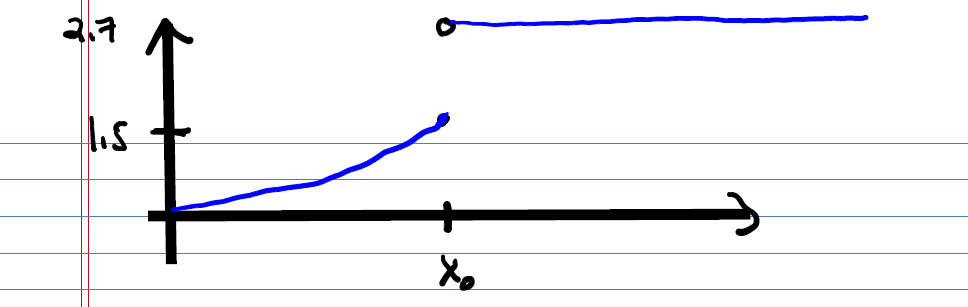
\includegraphics[width=0.7\columnwidth]{graphics/Chap06/Discontinuousfunction.png} }
    \caption[]{Let $\epsilon=1.0$ Then, $\forall~\delta>0, \exists~x\in B_\delta(x_0)$ such that $|f(x) - f(x_0)| \ge \epsilon$. Indeed, $x=x_0 +\delta_2$ works. }
    \label{fig:DiscontFunction}
\end{figure} 

\begin{definition} Let $\left(\mathcal{X},\| \bullet \|\right)$, and $\left(\mathcal{Y},||| \bullet |||\right)$ be normed spaces.
\begin{enumerate}
       \renewcommand{\labelenumi}{(\alph{enumi})}
        \setlength{\itemsep}{.1cm}
    \item $f:\mathcal{X} \to \mathcal{Y}$ is \textbf{ continuous at $x_0 \in \mathcal{X}$} if $\forall \epsilon > 0,~ \exists  \delta \left(\epsilon, x_0\right) > 0$ such that $ \|x-x_0\| < \delta \implies ||| f\left(x)\right) ||| < \epsilon.$
    
     \item $f$ is \textbf{ continuous} if it is continuous at $x_0$ for all $x_0 \in \mathcal{X}$.
 
\end{enumerate}

\end{definition} 

\begin{rem}
 It is also common to define continuity at a point as as $\forall ~\epsilon>0$, $\exists \delta>0$ such that $ x \in B_{\delta}\left(x_0\right) \implies  f\left(x\right) \in B_{\epsilon}\left(f\left( x_0\right)\right)$. Though less common, it can also be defined as $\forall ~\epsilon>0$, $\exists \delta>0$ such that $ f(B_{\delta}\left(x_0\right)) \subset  B_\epsilon(f(x_0))$.
\end{rem}

\begin{rem} \textbf{(Discontinuous at a point)} Let's negate the definition of $f$ continuous at $x_0$. $f$ is \textbf{discontinuous} at $x_0 \in \mathcal{X}$ if $\exists~\epsilon>0$ such that, $\forall~\delta >0, \exists ~x \in \mathcal{X}$ such that $||x-x_0||< \delta$ and $|||f(x) - f(x_0)||| \ge \epsilon$. This can also be stated as $\exists ~\epsilon>0$ such that, $\forall ~\delta>0$, $\exists~x \in B_\delta(x_0)$ such that $f(x) \not \in B_\epsilon(f(x_0))$. Finally, it can also be stated as $\exists ~\epsilon>0$, $\forall \delta>0$ such that $ f(B_{\delta}\left(x_0\right)) \not \subset  B_\epsilon(f(x_0))$.
\end{rem}

\begin{thm} \textbf{(Characterization of Continuity at a Point via Sequences)} Let  Let $\left(\mathcal{X},\| \bullet \|\right)$, and $\left(\mathcal{Y},||| \bullet |||\right)$ be normed spaces and $f:\mathcal{X} \to \mathcal{Y}$ a function.
    \begin{enumerate}
       \renewcommand{\labelenumi}{(\alph{enumi})}
        \setlength{\itemsep}{.1cm}
        \item If $f$ is continuous at $x_0$ and the sequence $\left(x_n\right)$ is a sequence in $\mathcal{X}$ that converges to $x_0$, then the sequence $(y_n:=f(x_n))$ in $\mathcal{Y}$ converges to $f(x_0)$. [$y_n:=f(x_n)$, $y_0:=f(x_0)$ implies $y_n \to y_0$ when $f$ is continuous at $x_0$. ]
        \item If $f$ is discontinuous at $x_0$, then there exists a sequence $\left(x_n\right)$ such that $ x_n \to x_0$, and $f\left(x_n\right) \not \to  f\left(x_0\right)$, that is, $f\left(x_n\right)$ does not converge to $f\left(x_0\right)$.
    \end{enumerate}
    
\end{thm} 

The proof is done in HW 10. The main point is, just as sequences can be used to completely characterize closed sets, they can also be used to completely characterize continuity at a point. 

\begin{cor} $f:\mathcal{X} \to \mathcal{Y}$ is continuous at $x_0$ if, and only if, every convergent sequence in $\mathcal{X}$ with limit $x_0$ is mapped by $f$ to a convergent sequence in $\mathcal{Y}$ with limit $f(x_0)$. In other symbols,  ($f$ is continuous at $x_0$)$\iff (x_n \to x_0 \implies f(x_n) \to f(x_0)).$ 

\end{cor}

\section{Compact Sets and the Existence of Extrema of Functions}

\begin{definition}  Let $(x_n)$ be a sequence and $1\le n_1<n_2<n_3<\dotsb $ be an infinite set of strictly increasing integers. Then, $(x_{n_i})$ is called a \textbf{ subsequence} of $(x_n)$. We note in passing that $n_i \ge i$, $\forall ~i\ge1$.
\end{definition}

\begin{example} $n_i = 2i + 1\textnormal{ or } n_i = 2^i.$
    
\end{example}

\begin{lem}
\label{lem:SubSequencesConverge}
 Suppose $x_n\to x$. Then every subsequence $(x_{n_i})$ of $(x_n)$ converges to $x$.
\end{lem}

We leave the proof as an exercise. 

\begin{definition} A set $S$ is \textbf{ bounded} if $\exists~ r < \infty$ such that $S \subset B_r(0)$.
\end{definition}

\begin{exercise} 
\label{exer:UnboundedStuff}
Show the following for $S\subset \mathcal{X}$:
\begin{enumerate}
    \item $S$ is bounded if, and only if, $\sup_{x\in S} \| x \| < \infty$.
     \item Hence, $S$ is unbounded if, and only if, $\sup_{x\in S} \| x \| = \infty$.
    \item $S$ is unbounded if, and only if, there exists a sequence $(x_k)$ such that, for all $k\ge 1$, $x_k\in S$ and $||x_{k+1}||\ge ||x_k|| + 1$.
\end{enumerate}
\end{exercise}

\begin{lem} If $S$ is unbounded, then it contains a sequence with no convergent subsequence.
\end{lem}

\textbf{Proof:} The sequence $(x_n)$ constructed above in Exercise~\ref{exer:UnboundedStuff} has no convergent subsequence. Indeed, by Remark~\ref{rem:HandyInequality}, if $(x_{n_i})$ is a subsequence of $(x_n)$, then $\| x_{n_i} -x_{n_j}\| \ge | ~\| x_{n_i}\| - \|x_{n_j}\|~| \ge |n_i - n_j|$, and thus is not Cauchy. Because it is not Cauchy, it cannot be convergent.

\Qed 

\begin{definition} \textbf{(Equivalent Norms)} Let $({\cal X}, \real)$ be a vector space. Two norms $||\cdot||:{\cal X} \to[0, \infty)$ and $|||\cdot|||:{\cal X} \to [0, \infty)$ are \textbf{equivalent} if there exist positive constants $K_1$ and $K_2$ such that, for all $x\in {\cal X}$,
    $$K_1 |||x||| \le ||x|| \le K_2 |||x|||. $$
\end{definition} 

\begin{rem}
It follows from the definition of equivalent norms that
$ \frac{1}{K_2}||x|| \le |||x||| \le \frac{1}{K_1} ||x||. $  
\end{rem}
-

We'll next develop a few bounds for norms on finite dimensional vector spaces, and use the bounds to relate convergence of a sequence of vectors in a finite dimensional normed space $(\mathcal{X}, ||\bullet ||)$ to the convergence of the representation of the sequence with respect to a basis. Let $\{v\}:=\{v^1, v^2, \ldots, v^n \}$ be a basis for $\mathcal{X}$ and define $M_i :=\spanof{v^j~| j \neq i}$, the $(n-1)$-dimensional subspace spanned by all the basis vectors except the $i$-th one. Because $M_i$ is finite dimensional, it is a complete and hence a closed subset of $\mathcal{X}$. By construction, $v^i \not \in M_i$, and thus, 
$$\delta_i:= d(v^i, M_i)>0. $$

\begin{lem} Let $\{v\}=\{v^1, v^2, \ldots, v^n \}$, $\{M_1, M_2, \ldots, M_n\}$ and $\{\delta_1, \delta_2, \ldots, \delta_n\}$ be as above. Then for any vector $x = \alpha_1 v^1+ \alpha_2 v^2 + \cdots + \alpha_n v^n \in \mathcal{X}$, 
\begin{equation}
\label{eq:equivalentNormsWithRepresentations}
    \kappa_\ast \left( \max_{1 \le i \le n} |\alpha_i| \right)  \le  ||x|| \le \kappa^\ast \left( \sum_{i=1}^n |\alpha_i| \right) \le n \kappa^\ast  \left( \max_{1 \le i \le n} |\alpha_i| \right),
\end{equation} 
where $\kappa_\ast:=\min_{1 \le i \le n}\{ \delta_i\}>0$, $\kappa^\ast := \max_{1 \le i \le n}\{ ||v^i||\} < \infty$, and $\alpha:=[x]_{\{v\}}$.

\end{lem}

\textbf{Proof:} The right hand side of \eqref{eq:equivalentNormsWithRepresentations} follows from the triangle inequality for norms. The proof of the left hand side of \eqref{eq:equivalentNormsWithRepresentations} requires a few steps that we carefully enumerate and leave to the reader:
\begin{enumerate}
    \item If $\alpha_i=0$, then $d(\alpha_i v^i, M_i) =0$. 
    \item If  $\alpha_i\neq 0$, then $d(\alpha_i v^i, M_i) = |\alpha_i|d(v^i, M_i) = |\alpha_i| \delta_i$.
    \item Hence, for all $\alpha_i \in \real$, $d(\alpha_i v^i, M_i) = |\alpha_i| \delta_i$
    \item For arbitrary $m_i \in M_i$, $d(\alpha_i v^i+m_i, M_i)=d(\alpha_i v^i-m_i, M_i)=d(\alpha_i v^i, M_i).$
    \item For any vector $x = \alpha_1 v^1+ \alpha_2 v^2 + \cdots + \alpha_n v^n \in \mathcal{X}$, $d(x, M_i) = d(\alpha_i v^i, M_i)$.
    \item Hence for any vector $x = \alpha_1 v^1+ \alpha_2 v^2 + \cdots + \alpha_n v^n \in \mathcal{X}$, and for all $1 \le i \le n$,
    $$||x|| \ge \inf_{m \in M_i} || x - m|| =: d(x, M_i) = |\alpha_i| \delta_i.$$
\end{enumerate}
\Qed

\begin{cor} \textbf{(Equivalent Norms)} All norms on finite dimensional vector spaces are equivalent\footnote{It is an interesting fact that a vector space is finite dimensional if, and only if, all norms on it are equivalent.}.
\end{cor}

\textbf{Proof:} Equation~\eqref{eq:equivalentNormsWithRepresentations} shows that, once a basis is chosen, any norm on an $n$-dimensional normed space is equivalent to $(\real^n, ||\bullet||_{\rm max})$. We leave it to the reader to show that this is enough to prove the result. 
\Qed

\begin{cor} \textbf{(Convergence of Components of Sequences in Finite-dimensional Spaces)}
\label{cor:Reduce2Reals}
Let $(x_k)$ be a sequence in a finite dimensional normed space $(\mathcal{X}, ||  \bullet ||)$ with basis $\{v^1, v^2, \ldots, v^n \}$. Let $$\mathbf{\alpha}_k:=[x_k]_{\{v\}} \in \real^n$$
be the representation of $x_k$ with respect to the basis $\{v\}$ so that 
$x_k =  \mathbf{\alpha}_{k,1} v^1+ \mathbf{\alpha}_{k,2} v^2 + \cdots + \mathbf{\alpha}_{k,n} v^n. $ Then $(x_k)$ is a Cauchy sequence in $\mathcal{X}$ if, and only if, each sequence $(\mathbf{\alpha}_{k,i})$ is a Cauchy sequence in $(\real, |\bullet |)$, $1 \le i \le n$.
\end{cor}

\textbf{Proof:} Equation~\eqref{eq:equivalentNormsWithRepresentations} reduces the proof to understanding that a sequence in $\real^n$ is Cauchy if, and only if, each of its real components is Cauchy. But with the max-norm, $(\real^n, ||\bullet||_{\rm max})$, this is quite easy to show because it selects the largest element, and if the largest element is getting small, then the rest of them are too. Have fun with it! 
\Qed

\begin{figure}[hbt!]%
	\centering{
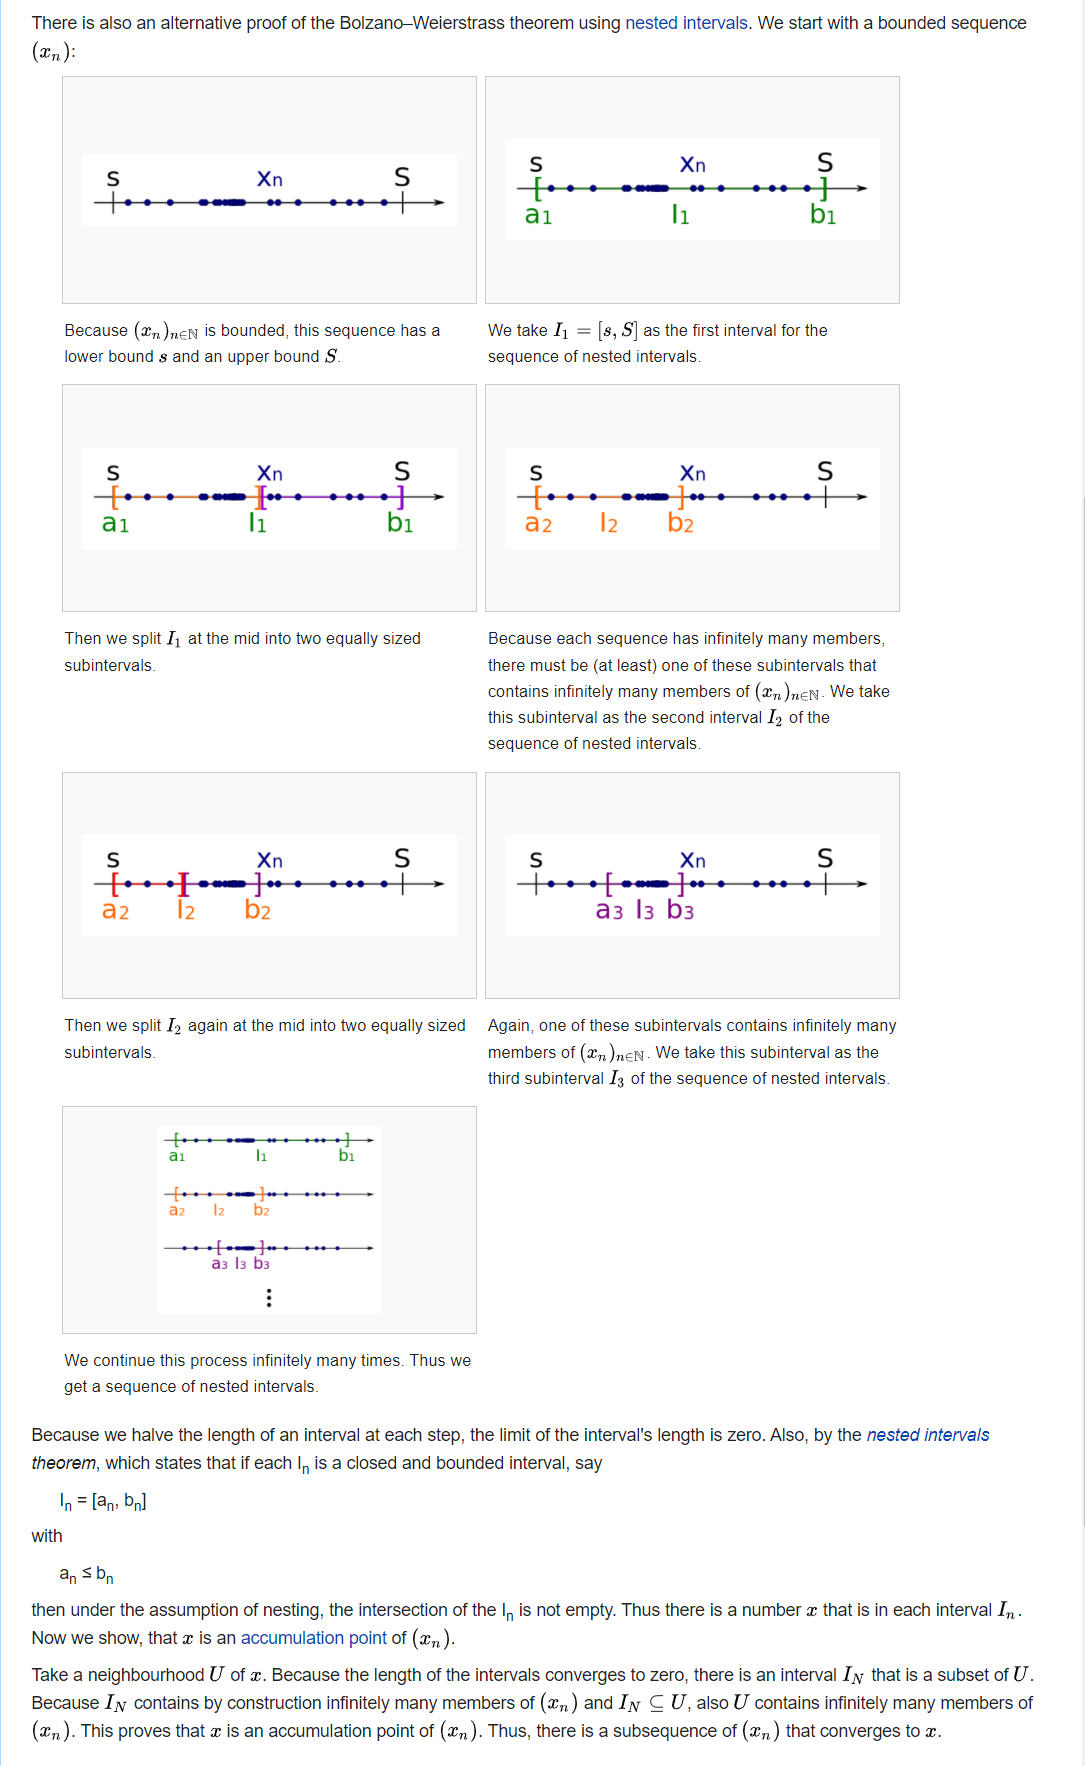
\includegraphics[width=0.72\columnwidth]{graphics/Chap06/BolzanoWeirstrassNestedIntervals.png} 
}
    \caption[]{ Illustration of a sequntial comactness proof from Wikipedia \url{https://en.wikipedia.org/wiki/Bolzano-Weierstrass_theorem}.}
    \label{fig:BolzanoWeirstrassProof}
\end{figure} 


\begin{thm} 
\label{thm:BolWeir}
\textbf{(Bolzano-Weierstrass Theorem or the Sequential Compactness Theorem)}~ In a finite dimensional normed space $(\mathcal{X}, ||  \bullet ||)$,
the following two properties are equivalent for a set $C \subset \mathcal{X}$.
\renewcommand{\labelenumi}{(\alph{enumi})}
\begin{enumerate}
\item $C$ is closed and bounded;
\item Every sequence in $C$ contains a convergent subsequence, that is, for every sequence $(x_n)$ in $C$ (i.e. $x_n \in C, \forall~n\ge 1$), there exists $x_0 \in C$ and a subsequence
$(x_{n_i})$ of $(x_n)$ such that $x_{n_i} \to x_0$.
\end{enumerate}
\end{thm}

\textbf{Proof:} We first show $\sim(a) \implies \sim (b)$. There are two cases, $C$ is not closed or $C$ is not bounded. \\

Suppose that $C$ is not closed. Then by Corollary~\ref{cor:ClosureAndLimitPoints}, there exists a limit point $x_0 \in \overline{C}$ such that $x_0 \not \in C$. Hence, there exists a sequence $(x_n)$ with $x_n \in C$ and $x_n \to x_0 \not \in C$. By Lemma~\ref{lem:SubSequencesConverge}, all subsequences $(x_{n_i})$ of $(x_n)$ satisfy $x_{n_i} \to x_0$. Hence, we have constructed a sequence of elements of $C$ for which there is no subsequence with a limit in $C$. \\

Suppose next that $C$ is unbounded. Then Exercise~\ref{exer:UnboundedStuff} produces a  sequence of elements of $C$ for which every subsequence is not Cauchy, and hence cannot have a limit in $C$. This completes the proof of $\sim(a) \implies \sim (b)$. Nothing we have done so far depends on $\mathcal{X}$ being finite dimensional.\\

We now turn to $(a) \implies (b)$. Let $(x_n)$ be an arbitrary sequence built from elements of $C$. To show: it has a convergent subsequence with limit in $C$.\\

\ul{Case 1:}  $(x_n)$ has only a finite number of distinct elements. Hence, at least one value is repeated an infinite number of times; let's call it $x_N \in C$. Because it is repeated an infinite number of times, we can choose a strictly increasing sequence $n_1 < n_2 < \cdots < n_i < \cdots$ such that $x_{n_i}=x_N$ for all $i \ge 1$. The subsequence $(x_{n_i})$ converges to $x_N \in C$ and hence we are done.\\

\ul{Case 2:} $(x_n)$ has an infinite number of distinct elements. Here, we will invoke that $\mathcal{X}$ is finite dimensional. Indeed, by Corollary~\ref{cor:Reduce2Reals}, a subsequence of $(x_n)$ will be convergent if, and only if, once it it is represented with respect to a basis, each of its components is convergent. Hence, it is enough to prove that every real sequence $(a_n)$, with an infinite number of distinct elements, contained in a closed and bounded subset of $C_1 \subset \real$ has a convergent subsequence. Every bounded subset of $\real$ is contained within a closed interval of the form $[-N, N]$, for some integer $1 \ge N < \infty$, and hence we reduce ourselves to a set $C_1 \subset [-N, N]$ and $C_1$ contains an infinite number of (distinct) elements of the sequence $(a_n)$. Because $C_1$ contains an infinite number of distinct elements of $(a_n)$, some closed interval of the form $[n, n+1]$, for $|n|\le N$ must contain an infinite number of elements of $(a_n)$. Without loss of generality, we will assume the closed interval $[0, 1]$ contains an infinite number of elements of $(a_n)$; the reader will see that our argument works \emph{mutatis mutandis} for any other interval of length one.\\

Divide the interval $[0, 1]$ into two halves, $[0, 1] = [0, 1/2] \cup [1/2, 1]$. At least one of the halves must contain an infinite number of elements of $(a_n)$. For the sake of argument, assume it is the right half. Now we divide in half $[1/2, 1] = [1/2, 3/4] \cup [3/4, 1]$ and note that at least one of the halves must contain an infinite number of elements of the sequence $(a_n)$. For the sake of argument, assume the left half this time. We then divide in half $[1/2, 3/4]=[1/2, 5/8] \cup [5/8, 3/4]$  and note that at least one of the halves must contain an infinite number of elements of the sequence $(a_n)$.\\

At the $k$-th step, we have a closed sub-interval of $I_k \subset [0, 1]$, with length $I_k$ equalling $1/2^k$ and $I_k$ contains an infinite number of distinct elements of $(a_k)$. Hence, for all $k\ge 1$, there exists $n_k$ such that $n_k > n_{k-1}$ and $a_{n_k} \in I_k$. Moreover, the sequence $(a_{n_k})$ is Cauchy because for all $i\ge k, j \ge k$, $|a_{n_i}- a_{n_j}| \le 1/2^k$. Hence the subsequence $(a_{n_k})$ converges to a limit in $C_1$ and the proof is done.

\Qed


\begin{definition} A set $C$ satisfying (a) or (b) of Theorem~\ref{thm:BolWeir} is said to be \textbf{ compact}. 
\end{definition}.


\begin{rem}
There are various definitions of compactness that are appropriate for specific settings. The one above is typically called sequential compactness. Because it is the only form of compactness we use in these notes, we will drop the term sequential and simply call such sets compact sets. 
\end{rem}


\begin{thm} \textbf{(Weierstrass Theorem)}~ If $C$ is compact and $f: C \to \real$ is continuous, then $f$ achieves its extreme values. That is,
    \begin{equation*}
        \exists x^\ast \in C\textnormal{, s.t. }f(x^\ast)=\sup\limits_{x\in C}f(x)
    \end{equation*}
    and
    \begin{equation*}
        \exists x_* \in C\textnormal{, s.t. }f(x_*)=\inf\limits_{x\in C}f(x).
    \end{equation*}

\end{thm}

\textbf{Proof:}~ Let $f^\ast:=\sup\limits_{x\in C}f(x)$. To show $\exists x^\ast \in C$, such that $f(x^\ast)=f^\ast$.\\

\begin{claim} $f^\ast$ is finite.
\end{claim}

{Proof:} We do a proof by contradiction and suppose not, that is, suppose $f^\ast = \infty$. Then, by definition of the supremum, for all $n\ge 1$, there exists $x_n \in C$ such that $f(x_n) \ge n$. Because $C$ is compact, there exists $x_0 \in C$ and a subsequence $(x_{n_i})$ of $(x_n)$ such that
$x_{n_i} \to x_0$. Because $f$ is assumed continuous, 
$$f(x_0) = \lim_{i \to \infty} f(x_{n_i}) \ge   \lim_{i \to \infty} n_i = \infty.$$
But because $f:C \to \real$, $f(x_0) \in \real$, which contradicts $f(x_0) = \infty$. Hence, it cannot be the case that $f^\ast = \infty$.

$\hfill \square$

Continuing with the proof, we now know that $f^\ast$ is finite. Once again, applying the definition of the supremum, we have that $\forall n>0, \exists ~x_n\in C$ such that $|f^\ast-f(x_n) |<1/n$. Because
    $C$ is compact,  there exists $x^\ast \in C$ and a subsequence $(x_{n_i})$ such that 	$x_{n_i} \to x^\ast$. Because $f$ continuous, $f(x_{n_i})\to f(x^\ast)$. We expect to show that $f(x^\ast) = f^\ast$. To do so, we note that, by the continuity\footnote{Technically, we are using the continuity of $f$ implies that of $g(x):=|f^\ast - f(x)|$, which you are welcome to check. Otherwise, you can do the estimate as $|f^\ast -f(x^\ast)| =|f^\ast - f(x_{n_i}) + f(x_{n_i})- f(x^\ast)| \le  |f^\ast - f(x_{n_i})| + |f(x_{n_i}) - f(x^\ast)|  \le \frac{1}{n_i} + |f(x_{n_i}) - f(x^\ast)|  \xrightarrow[i\to \infty]{}0.$ } of $f$,
$$|f^\ast -f(x^\ast)|= \lim_{i \to \infty} |f^\ast - f(x_{n_i})|  \le  \lim_{i \to \infty} \frac{1}{n_i}=0. $$
And hence, 
    $f^\ast=f(x^\ast)$.\\
    
    The same proof works for the infimum. 
    
    \Qed



\chapter{Briefest of Remarks on Optimization}
\label{chap:Optimization}

\section*{Learning Objectives}

\begin{itemize}
\item Learn about ``convexity'', which defines a class of problems where local minima are also global minima
\item Learn about two types of convex optimization problems that are fast enough to run in real time on many mobile platforms.
\end{itemize}

\section*{Outcomes} 
\begin{itemize}
\item  Definition of convex sets and convex functions.
\item Local minima of convex functions are also global minima.
\item A Quadratic Program (QP) is an optimization problem with a quadratic cost and linear inequality and equality constraints.
\item A Linear Program (LP) is an optimization problem with a linear cost and linear inequality and equality constraints.
\item Through the concept of ``slack variables'', an optimization problem with either a one-norm or $\infty$-norm as the the cost and linear inequality and equality constraints can be turned into an LP.
\end{itemize}

\newpage

\section{Brief Remarks on Convex Sets and Convex Functions}

\begin{definition}  Let $(\mathcal{X},\real)$ be a real vector space. $C \subset V$ is \textbf{ convex} if $\forall x,y \in C $ and $ 0\le \lambda \le 1$, the \textbf{convex combination} $\lambda x +(1-\lambda)y \in C$.

\end{definition}


\begin{rem} 
$$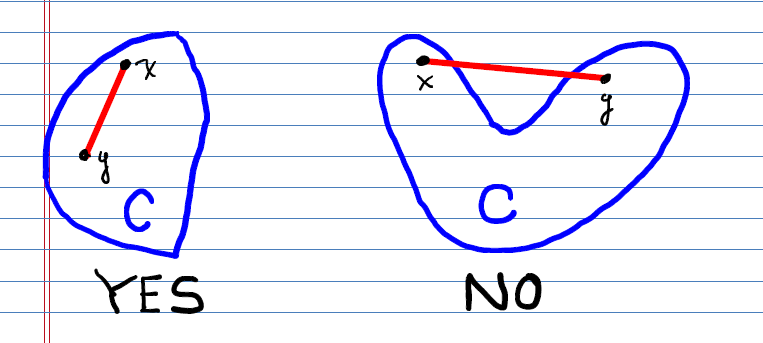
\includegraphics[width=0.70\columnwidth]{graphics/Chap06/ConvexSet.png} $$
\renewcommand{\labelenumi}{(\alph{enumi})}
\begin{enumerate}
\item For $C$ to be convex, given any two points $x,y \in C$, then the line connecting $x$ and $y$ must also lie in $C$.
\item Open and closed balls arsing from norms are always convex. 
\end{enumerate}
\end{rem}

\begin{definition} The \textbf{convex hull} of a set $S \subset \mathcal{X}$ is
$${\rm co}(S):=\{ \lambda x + (1 - \lambda)y ~|~ 0 \le \lambda \le 1, x, y \in S\}, $$
the set of all convex combinations of elements of $S$. It can also be defined as the smallest convex set that contains $S$. 
\end{definition}
$$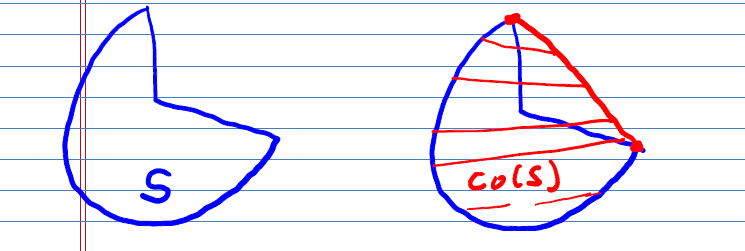
\includegraphics[width=0.70\columnwidth]{graphics/Chap06/ConvexHull.png} $$

\begin{definition} Suppose $C\subset \mathcal{X}$ is convex. A function
$f:C\to \real$ is \textbf{ convex} if $~\forall x,y \in C, 0 \le \lambda \le 1$,
$$f\left(\lambda x+(1-\lambda) y\right)\le \lambda f(x)+(1-\lambda)f(y).$$
\end{definition}
$$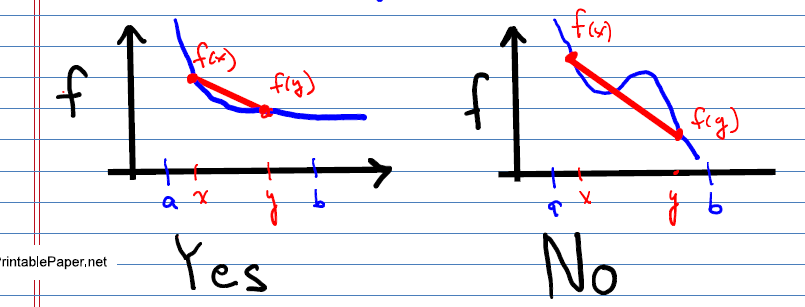
\includegraphics[width=0.70\columnwidth]{graphics/Chap06/ConvexFunction.png} $$

\begin{rem} For a function to be convex, the line $\lambda x + (1 - \lambda)y$ connecting $x$ and $y$ must lie at or above the graph of the function; it can never go below.

\end{rem}


\begin{definition} Suppose $(\mathcal{X},\real,||  \bullet ||)$ is a normed space, $D\subset \mathcal{X}$ a subset, and $f:D\to \real$ a function.
\renewcommand{\labelenumi}{(\alph{enumi})}
\begin{enumerate}
\item
$x^\ast \in D$ is a \textbf{ local minimum} of $f$ if $\exists \delta >0$ such that $\forall x\in B_\delta(x^\ast)$,
$f(x^\ast) \le f(x)$.
\item
$x^\ast \in D$ is a \textbf{ global minimum} if $\forall y \in D$, $f(x^\ast) \le f(y)$.
\end{enumerate}

\end{definition}

\begin{thm}\textbf{(Local equals Global for Convex Functions)} If $D$ and $f$ are both convex, then any local minimum is also a global minimum.
\end{thm} 

\textbf{ Proof:}~  We show that if $x$ is not a global minimum, then it cannot be a local minimum. Specifically, we prove the contrapositive statement: $((a) \implies (b)) \iff (\lnot (b) \implies \lnot (a))$, where
\begin{enumerate}
       \renewcommand{\labelenumi}{(\alph{enumi})}
        \setlength{\itemsep}{.1cm}
    \item $x\in D$ is a local minimum
    \item $x \in D$ is a global minimum.
       
    \item[$\lnot$(b)] $\exists y \in D$ such that $f(y) < f(x)$.
    
     \item[$\lnot$(a)] $\forall~\delta>0, \exists~z\in B_\delta(x) \cap D$ such that $f(z) < f(x)$.
\end{enumerate}

\begin{claim} If $f(y) < f(x)$, then $\forall  0<\lambda\le 1$, the vector  $z:=(1-\lambda)x+\lambda y$ satisfies $f(z) < f(x)$.
\end{claim}

Proof:  
\begin{align*}
        f(z)&=f((1-\lambda)x+\lambda y)\\
        &\le (1-\lambda)f(x)+\lambda f(y) ~~[\text{convexity}]\\
        &<(1-\lambda)f(x)+\lambda f(x)~~ [f(x) > f(y)]\\
        &=f(x).
    \end{align*}
    Hence, $f(z) < f(x)$.
    $\hfill \square$

\begin{claim} $\forall \delta >0$, $\exists 0 < \lambda < 1$ such that $z:=(1-\lambda)x+\lambda y \in B_\delta(x) \cap D$.
\end{claim}
Proof:
    \begin{align*}
        ||z-x||&=||(1-\lambda)x+\lambda y-x||\\
        &=||\lambda(y-x)||\\
        &=\lambda||y-x||
    \end{align*}
Therefore, if $ 0 < \lambda < \max\{\frac{\delta}{||y-x||}, 1\}$, then $||z - x|| < \delta$, and hence $z \in  B_\delta(x)$. Because $D$ is convex, $z \in D$. Hence, $z \in  B_\delta(x)\cap D$.

    $\hfill \square$\\
    
    The two Claims establish $\lnot (b) \implies \lnot (a)$, and hence the proof is complete.
    
    \Qed

\begin{fact}\mbox{ }
\begin{itemize}
        \item All norms $\| \bullet \|:\mathcal{X} \to [0, \infty)$ are convex.
        
        \item For all $1\leq\beta<\infty$, $\| \bullet \|^\beta$ is convex. Hence, on $\real^n$, $\forall~ 1 \le p < \infty$, $ \Sigma_{i=1}^{n}|x_i|^p$            is convex.
        \item Let $r>0$, $\| \bullet \|$ a norm, $B_r(x_0)$ is a convex set; special case: $B_1(0)$ convex set. (unit ball about the origin).
        \item Let $C$ be an open, bounded and convex set, 0 $\in$ C. Then, $\exists\ \| \bullet \|: X \to [0,\infty)$ such that $C=\{x\in \mathcal{X}\ |\:||x||<1\} = B_1(0)$. In other words, open unit balls are characterized by the fact that they are open, bounded, convex sets that contain the origin. 
        \item $K_1$ and $K_2$ are convex, then $K_1 \cap K_2$ is convex. (by convention, the empty set is convex)
        \item Consider $(\real^n, \real)$ and let $A$ be a real $m \times n$ matrix and $b\in \real^m$. Then,
        \begin{itemize}
            \item $K_1=\{x \in \real^n|\:Ax\leq b\}$ is also convex (linear inequality with $Ax\leq b$ interpreted row wise).
            \item $K_2=\{x \in \real^n|\:Ax=b\}$ is convex (linear equality).
            \item $K_3=\{x \in \real^n|\:A_{eq}x=b_{eq},\ A_{in}x\leq b_{in}\}$ is convex as well by the intersection property.
        \end{itemize}
    \end{itemize}

\end{fact}
    

\begin{rem} $\widetilde{A}x \geq \widetilde{b} \iff (-\widetilde{A})x \leq (-\widetilde{b})$.

\end{rem}


\begin{fact} \textbf{(Not an Easy one to Prove)} Suppose $(\mathcal{X},\real,||  \bullet ||)$ is a finite dimensional normed space, $C\subset \mathcal{X}$ is convex, and $f:C\to \real$ is convex. Then $f$ is continuous on $\mathring C$.
\end{fact}   

\begin{rem} $f$ can have jumps on the boundary of $C$, that is, on $\partial C:= \overline{C} \cap \overline{(\sim C)} = \overline{C} \setminus \mathring{C} := \{ x \in \overline{C}~|~ x \not \in \mathring{C}\}$.
\end{rem}
    
\section{Remarks on Notation and Abuse of Notation}

Let $(\mathcal{X}, \real, \|\bullet\|)$ be a real normed space, $S \subset \mathcal{X}$, and $f:S \to \real$. It is very common to write
\begin{equation}
\label{eq:ArgMinNotation}
    x^\ast = \argmin_{x \in S} f(x)
\end{equation}
for the value of $x\in S$ that achieves the minimum of $f$ over all possible elements of $S$; that is, $f(x^\ast) = \min_{x \in S} f(x)$. Now, the problem is, you should only write something like \eqref{eq:ArgMinNotation} when
\begin{enumerate}
    \item There does exist a minimum value, and 
    \item it is unique.
\end{enumerate}
If a minimum exists but is not unique, one should write
\begin{equation}
\label{eq:ArgMinNotation02}
    x^\ast \in \argmin_{x \in S} f(x)
\end{equation}
to indicate that $x^\ast$ is one of a set of values that all minimize the function $f$ over the set $S$. It is correct notation, but not commonly used. If you are not sure that a minimum exists, then definitely you should not use \eqref{eq:ArgMinNotation}. Even worse,  \textcolor{red}{\bf something you should never do is write }
\begin{equation}
\label{eq:ArgMinNotation02}
    x^\ast = \arg~\inf_{x \in S} f(x)
\end{equation}
because it makes no sense! By the very definition of an infimum, there may be no value in $S$ achieving the infimum. \\

In \eqref{eq:ArgMinNotation}, $f$ is called the \textbf{cost function} and $S$ is the \textbf{constraint set.}

\section{What is a Quadratic Program?}

Example~\ref{ex:OverDetermined} and Proposition~\ref{prop:UnderDetermined} dealt with least squares solutions of overdetermined systems of linear equations 
$$\widehat{x} = \argmin_{x} (A x -b)^\top Q (Ax-b), $$
 with $Q$ a positive definite matrix, while Theorem~\ref{thm:BestApproxLinearVariety} and Proposition~\ref{prop:WLS} dealt with minimum norm squared solutions of underdetermined systems of linear equations 
  $$\widehat{x}:= \argmin_{Ax=b} x^\top Q x. $$
  These are both quadratic optimization problems that admit closed-form solutions. \\

A \textbf{Quadratic Program} is a more general kind of quadratic optimization problem with constraints. The cost to be minimized in \eqref{eq:ArgMinNotation} is quadratic plus a linear term, meaning that $f:\real^m \to \real $ has the form
\begin{equation}
    \label{eq:QPconst}
    f(x) = \frac{1}{2} x^\top Q x + q x, 
\end{equation}
where $Q$ is an $m\times m$ symmetric, positive \textbf{semi-definite} matrix, and $q$ is a $1 \times m$ row vector. Moreover, instead of optimizing over all of $\real^m$ as in Example~\ref{ex:OverDetermined} and Proposition~\ref{prop:UnderDetermined}, or only over linear equality constrains, as in Theorem~\ref{thm:BestApproxLinearVariety} and Proposition~\ref{prop:WLS}, we are allowed to seek solutions that lie in a subset of $\real^m$ defined by \textbf{linear inequality} and \textbf{linear equality} constraints that are typically written in the form
\begin{align}
\label{eq:QPconstraintsInequality}
   A_{in} x & \preceq b_{in} \\
   \label{eq:QPconstraintsEquality}
   A_{eq} x & = b_{eq}.
\end{align}
Recall that the symbol $\preceq$ is a way to define ``less than or equal to'' for vectors; it means that each component of the vector on the left hand side is less than or equal to the corresponding component of the vector on the right hand side. As an example 
$$\begin{bmatrix}3 \\ 2 \\ 4\end{bmatrix} \preceq \begin{bmatrix}4 \\ 3 \\ 4\end{bmatrix},  $$
   though 
$$\begin{bmatrix}3 \\ 2 \\ 4\end{bmatrix} \not \preceq \begin{bmatrix}1 \\ 3 \\ 4\end{bmatrix};  $$ 
and 
$$\begin{bmatrix}3 & 1 \\ 2 & 4\end{bmatrix}\begin{bmatrix}x_1 \\ x_2 \end{bmatrix} \preceq \begin{bmatrix}0 \\ 9\end{bmatrix},  $$
means that $x_1$ and $x_2$ must satisfy
$$\begin{aligned} 3 x_1 + x_2 &\le 0  \\ 2 x_1 + 4 x_2 &\le 9. \end{aligned} $$
What if you really wanted $2 x_1 + 4 x_2 \ge 9$? Then you need to remember that when you multiply both sides by a minus sign, the inequality sign flips. Hence,
$$\begin{aligned} 3 x_1 + x_2 &\le 0  \\ 2 x_1 + 4 x_2 &\ge 9 \end{aligned} \iff \begin{aligned} 3 x_1 + x_2 &\le 0  \\ -2 x_1 - 4 x_2 &\le -9 \end{aligned} \iff  \left[
\begin{array}{rr}
3 & 1\\ -2 & -4
\end{array} \right] \begin{bmatrix}x_1 \\ x_2 \end{bmatrix} \preceq \left[
\begin{array}{r}
0 \\ -9
\end{array}
\right].$$
In addition, most QP solvers allow one to specify lower and upper bounds on $x$ of the form
\begin{align}
\label{eq:QPconstraintsUpperLower}
   lb \preceq x \preceq ub.
\end{align}
While such constraints could always be rewritten in the form of \eqref{eq:QPconstraintsInequality}, using \eqref{eq:QPconstraintsUpperLower} is more convenient, intuitive, and less error prone. The inclusion of constraints allows for very interesting and practical optimization problems to be posed. 

\vspace*{0.5cm}

\begin{tcolorbox}[title=\textbf{Useful Fact about QPs}]
We consider the QP 
\begin{equation}
    \label{eq:QPnominalForm}
        x^\ast = \argmin_{
        \begin{aligned} x &\in \real^m \\
     A_{in} x & \preceq b_{in} \\
     A_{eq} x & = b_{eq} \\
     lb \preceq &~~x \preceq ub \end{aligned}
     } \frac{1}{2} x^\top Q x + qx
\end{equation}
and assume that $Q$ is symmetric ($Q^\top = Q$) and \textbf{positive definite} ($x \neq 0 \implies x^\top Q x >0$), and that the subset of $\real^m$ defined by the constraints is non empty, that is
\begin{equation}
    \label{eq:QPconstraintsNotEmpty}
S:=\{x \in \real^m~|~ A_{in} x  \preceq b_{in},~  A_{eq} x  = b_{eq},~ lb \preceq x \preceq ub  \} \neq \emptyset.
\end{equation} 
Then $x^\ast$ exists and is unique. 
\end{tcolorbox}
    
There are special purposes solvers available for QPs. 
\begin{itemize}
    \item \url{https://www.ibm.com/docs/en/icos/20.1.0?topic=qp-optimizing-qps}
    \item \url{https://github.com/osqp/OSQP.jl}
    \item \url{https://web.stanford.edu/~boyd/papers/pdf/osqp.pdf}
    \item \url{https://stanford.edu/~boyd/software.html}
    \item \url{https://www.mathworks.com/help/optim/ug/quadprog.html}
    \item \url{https://www.mathworks.com/help/mpc/ug/qp-solver.html}
\end{itemize}

\vspace*{.2cm} 
How do QPs arise in Robotics? Here is one example. 
Consider the robot equations,
        \begin{equation*}
            D(q)\ddot{q}+C(q,\dot{q})\dot{q}+G(q) = Bu
        \end{equation*}
    where $q \in \real^n$, $u\in \real^m$. The ground reaction forces for a bipedal robot can be expressed as
        \begin{equation*}
            F = \Lambda_0(q,\dot{q})+\Lambda_1(q)u = \left[ \begin{array}{c}
												F^h \\
                                                F^v \end{array} \right].
        \end{equation*}
        
Suppose the commanded torque is $u=\gamma(q,\dot{q})$ and we need to respect bounds on the ground reaction forces, such as
        \begin{equation*}
            F^v \geq 0.2m_{total}g,
        \end{equation*}
which means the normal force should be at least $20\%$ of the total weight of the robot, and 
        \begin{equation*}
            |F^h| \leq 0.6F^v,
        \end{equation*}
which places the horizontal component of the ground reaction force in a friction cone with magnitude less than $60\%$ of the total vertical force. Putting it all together:
        \begin{equation*}
            \left[ \begin{array}{rl}
		        F^v &\geq 0.2m_{total}g\\
                F^h  & \leq 0.6F^v\\
                -F^h &\leq 0.6F^v\end{array} \right]
                \iff A_{in} (q)u\leq b_{in}(q,\dot{q}).
        \end{equation*}

    \textbf{QP:}
    \begin{equation*}
        u^\ast = \operatorname{argmin}\ u^\top u + p\ d^\top d
    \end{equation*}
    \begin{align*}
        A_{in}(q)u & \leq b_{in}(q,\dot q) \\
         u& = \gamma(q, \dot{q})+d,
    \end{align*}
where $d$ is a relaxation parameter that allows the torque to deviate from its desired value in order to respect the constraints on the ground reaction forces. The parameter $p$ is a scalar weight term.

\section{What is a Linear Program and How can it be used to Minimize $|| \bullet||_1$ and $|| \bullet||_{\rm max}$?}

\begin{definition} A \textbf{Linear Program} means to minimize a scalar-valued linear function subject to linear equality and inequality constraints. For $x \in \real^n$, and $f \in \real^n$
\begin{align*}
\text{minimize}& ~~ f^\top x\\
\text{subject to} &~~A_{in} x \preceq b_{in} \\
 & ~~A_{eq} x = b_{eq}
\end{align*}
where $A_{in} x \preceq b_{in}$ means each row of $A_{in}x$ is less than or equal to the corresponding row of $b_{in}$. The only restrictions on $A_{in}$ and $A_{eq}$ are that the set 
$$K=\{ x \in \real^n~|~ A_{in} x \preceq b_{in},~ A_{eq} x = b_{eq} \}$$
should be non-empty.
\end{definition}
% \vspace*{2cm}
% \noindent \textbf{Remarks:} Below is the MATLAB function call. Typically, the inequality constraints are not written with a subscript ${in}$. The next pages will show why I am doing this.
% \begin{verbatim}
%     X = linprog(f,A,b) attempts to solve the linear programming problem:

%              min f'*x    subject to:   A*x <= b
%               x

%     X = linprog(f,A,b,Aeq,beq) solves the problem above while 
%     satisfying the equality constraints Aeq*x = beq.
% \end{verbatim}


% \newpage

Remarkably, through a concept called \textbf{slack variables}, Linear Programs can be applied to cost functions that include the one-norm and the max-norm.

\begin{tcolorbox}[title = Linear Program for ${ \bf\ell}_1$-\textbf{norm:} {$||x||_1 = \sum_{i=1}^{n} |x_i|$}]

Suppose that $A$ is an $m \times n$ real matrix. Minimize $||Ax - b||_1$ is equivalent to the following linear program on $\real^{n+m}$

\begin{equation}
\label{eq:ell1normviaLP}
\begin{aligned}
\text{minimize}& ~~ f^\top X\\
\text{subject to} &~~A_{in} X \preceq b_{in} \\
\end{aligned}
\end{equation}

with $X = \left[\begin{array}{c}  x\\ s \end{array} \right]$ ($s\in \real^m$ are called slack variables)


$$f:=\left[ \begin{array}{cc}0_{1 \times n} & \textbf{1}_{1 \times m} \end{array} \right],~~A_{in}:= \left[ \begin{array}{rr}  A  & -I_{m \times m}  \\
 -A  & -I_{m \times m}\end{array} \right] ~~\text{and}~~ b_{in}:=\left[\begin{array}{r}  b\\ -b \end{array} \right]$$

If $\widehat{X}=[\widehat{x}^\top, ~ \widehat{s}^\top ]^\top $  is the solution of the linear programming problem, then $\widehat{x}$ solves the 1-norm optimization problem; that is
$$ \widehat{x} \in {\rm arg}~\min_{x \in \real^n} ||Ax - b||_1.$$
 \end{tcolorbox}
 
 \vspace*{.2cm}

Let's see if we can understand why the above is true. Writing out the terms, equation \eqref{eq:ell1normviaLP} becomes
\begin{align*}
\underset{x, s}{\text{minimize}}& ~~ \sum_{i=1}^m s_i \\
\text{subject to} &~~~~\ A x -s \preceq b \\
                 &-A x -s \preceq -b.\\
\end{align*}
This is equivalent to 
\begin{align*}
\underset{x, s}{\text{minimize}}& ~~ \sum_{i=1}^m s_i \\
\text{subject to} &-s \preceq b -Ax\\
                 & -s \preceq -(b - Ax),\\
\end{align*}
which is equivalent to
\begin{align*}
\underset{x, s}{\text{minimize}}& ~~ \sum_{i=1}^m s_i \\
\text{subject to} &-s \preceq b -Ax\\
                 & +s \succeq b - Ax,\\
\end{align*}
which is equivalent to
\begin{align*}
\underset{x, s}{\text{minimize}}& ~~ \sum_{i=1}^m s_i \\
\text{subject to} &-s \preceq b -Ax \preceq s.
\end{align*}
Because for real numbers $s_i, y_i$, the inequality $(-s_i\le y_i \le s_i) \iff (0 \le |y_i| \le s_i) $,
we end up with 
\begin{align*}
\underset{x, s}{\text{minimize}} & ~~ \sum_{i=1}^m s_i \\
\text{subject to} &~~ 0\le  |b -Ax|_i \le  s_i,
\end{align*}
which is equivalent to
\begin{align*}
\underset{x}{\text{minimize}} & ~~ \sum_{i=1}^m  |b -Ax|_i. 
\end{align*}

Whoever thought this up was pretty clever! It reduces a nonlinear problem to a linear problem. The max-norm is a bit simpler, requiring only a single slack variable.

\vspace*{.2cm}

\begin{tcolorbox}[title = Linear Program for ${\bf\ell}_\infty$-\textbf{norm:} {$||x||_\infty = \max_{1 \le i \le n} |x_i| $}]

Suppose that $A$ is an $m \times n$ real matrix. Minimize $||Ax - b||_\infty$ is equivalent to the following linear program on $\real^{n+1}$

\begin{align*}
\text{minimize}& ~~ f^\top X\\
\text{subject to} &~~A_{in} X \preceq b_{in} \\
\end{align*}

with $X = \left[\begin{array}{c}  x\\ s \end{array} \right]$ ($s\in \real$ is called a slack variable)

%%$$f:=\left[ \begin{array}{cc}0_{1 \times n} & 1 \end{array} \right]$$
$$f:=\left[ \begin{array}{cc}0_{1 \times n} & 1 \end{array} \right], ~~A_{in}:= \left[ \begin{array}{rr}  A  & -\textbf{1}_{m \times 1}  \\
 -A  & -\textbf{1}_{m \times 1}\end{array} \right] ~~\text{and}~~ b_{in}:=\left[\begin{array}{r}  b\\ -b \end{array} \right]$$

If $\widehat{X}=[\widehat{x}^\top, ~ \widehat{s} \ ]^\top $  solves the linear programming problem, then  $\widehat{x}$ solves the max-norm optimization problem; that is
$$ \widehat{x} \in  {\rm arg}~~\min_{x \in \real^n} ||Ax - b||_\infty.$$
\end{tcolorbox} 

\pagestyle{plain}

% \newpage

% \appendix

% \chapter{To Learn on Your Own (if you want to): Cool and Important Things We Omitted From our Linear Algebra Introduction}


\end{document}

